% Options for packages loaded elsewhere
\PassOptionsToPackage{unicode}{hyperref}
\PassOptionsToPackage{hyphens}{url}
\PassOptionsToPackage{dvipsnames,svgnames,x11names}{xcolor}
%
\documentclass[
  letterpaper,
  DIV=11,
  numbers=noendperiod]{scrartcl}

\usepackage{amsmath,amssymb}
\usepackage{iftex}
\ifPDFTeX
  \usepackage[T1]{fontenc}
  \usepackage[utf8]{inputenc}
  \usepackage{textcomp} % provide euro and other symbols
\else % if luatex or xetex
  \usepackage{unicode-math}
  \defaultfontfeatures{Scale=MatchLowercase}
  \defaultfontfeatures[\rmfamily]{Ligatures=TeX,Scale=1}
\fi
\usepackage{lmodern}
\ifPDFTeX\else  
    % xetex/luatex font selection
\fi
% Use upquote if available, for straight quotes in verbatim environments
\IfFileExists{upquote.sty}{\usepackage{upquote}}{}
\IfFileExists{microtype.sty}{% use microtype if available
  \usepackage[]{microtype}
  \UseMicrotypeSet[protrusion]{basicmath} % disable protrusion for tt fonts
}{}
\makeatletter
\@ifundefined{KOMAClassName}{% if non-KOMA class
  \IfFileExists{parskip.sty}{%
    \usepackage{parskip}
  }{% else
    \setlength{\parindent}{0pt}
    \setlength{\parskip}{6pt plus 2pt minus 1pt}}
}{% if KOMA class
  \KOMAoptions{parskip=half}}
\makeatother
\usepackage{xcolor}
\setlength{\emergencystretch}{3em} % prevent overfull lines
\setcounter{secnumdepth}{5}
% Make \paragraph and \subparagraph free-standing
\makeatletter
\ifx\paragraph\undefined\else
  \let\oldparagraph\paragraph
  \renewcommand{\paragraph}{
    \@ifstar
      \xxxParagraphStar
      \xxxParagraphNoStar
  }
  \newcommand{\xxxParagraphStar}[1]{\oldparagraph*{#1}\mbox{}}
  \newcommand{\xxxParagraphNoStar}[1]{\oldparagraph{#1}\mbox{}}
\fi
\ifx\subparagraph\undefined\else
  \let\oldsubparagraph\subparagraph
  \renewcommand{\subparagraph}{
    \@ifstar
      \xxxSubParagraphStar
      \xxxSubParagraphNoStar
  }
  \newcommand{\xxxSubParagraphStar}[1]{\oldsubparagraph*{#1}\mbox{}}
  \newcommand{\xxxSubParagraphNoStar}[1]{\oldsubparagraph{#1}\mbox{}}
\fi
\makeatother

\usepackage{color}
\usepackage{fancyvrb}
\newcommand{\VerbBar}{|}
\newcommand{\VERB}{\Verb[commandchars=\\\{\}]}
\DefineVerbatimEnvironment{Highlighting}{Verbatim}{commandchars=\\\{\}}
% Add ',fontsize=\small' for more characters per line
\usepackage{framed}
\definecolor{shadecolor}{RGB}{241,243,245}
\newenvironment{Shaded}{\begin{snugshade}}{\end{snugshade}}
\newcommand{\AlertTok}[1]{\textcolor[rgb]{0.68,0.00,0.00}{#1}}
\newcommand{\AnnotationTok}[1]{\textcolor[rgb]{0.37,0.37,0.37}{#1}}
\newcommand{\AttributeTok}[1]{\textcolor[rgb]{0.40,0.45,0.13}{#1}}
\newcommand{\BaseNTok}[1]{\textcolor[rgb]{0.68,0.00,0.00}{#1}}
\newcommand{\BuiltInTok}[1]{\textcolor[rgb]{0.00,0.23,0.31}{#1}}
\newcommand{\CharTok}[1]{\textcolor[rgb]{0.13,0.47,0.30}{#1}}
\newcommand{\CommentTok}[1]{\textcolor[rgb]{0.37,0.37,0.37}{#1}}
\newcommand{\CommentVarTok}[1]{\textcolor[rgb]{0.37,0.37,0.37}{\textit{#1}}}
\newcommand{\ConstantTok}[1]{\textcolor[rgb]{0.56,0.35,0.01}{#1}}
\newcommand{\ControlFlowTok}[1]{\textcolor[rgb]{0.00,0.23,0.31}{\textbf{#1}}}
\newcommand{\DataTypeTok}[1]{\textcolor[rgb]{0.68,0.00,0.00}{#1}}
\newcommand{\DecValTok}[1]{\textcolor[rgb]{0.68,0.00,0.00}{#1}}
\newcommand{\DocumentationTok}[1]{\textcolor[rgb]{0.37,0.37,0.37}{\textit{#1}}}
\newcommand{\ErrorTok}[1]{\textcolor[rgb]{0.68,0.00,0.00}{#1}}
\newcommand{\ExtensionTok}[1]{\textcolor[rgb]{0.00,0.23,0.31}{#1}}
\newcommand{\FloatTok}[1]{\textcolor[rgb]{0.68,0.00,0.00}{#1}}
\newcommand{\FunctionTok}[1]{\textcolor[rgb]{0.28,0.35,0.67}{#1}}
\newcommand{\ImportTok}[1]{\textcolor[rgb]{0.00,0.46,0.62}{#1}}
\newcommand{\InformationTok}[1]{\textcolor[rgb]{0.37,0.37,0.37}{#1}}
\newcommand{\KeywordTok}[1]{\textcolor[rgb]{0.00,0.23,0.31}{\textbf{#1}}}
\newcommand{\NormalTok}[1]{\textcolor[rgb]{0.00,0.23,0.31}{#1}}
\newcommand{\OperatorTok}[1]{\textcolor[rgb]{0.37,0.37,0.37}{#1}}
\newcommand{\OtherTok}[1]{\textcolor[rgb]{0.00,0.23,0.31}{#1}}
\newcommand{\PreprocessorTok}[1]{\textcolor[rgb]{0.68,0.00,0.00}{#1}}
\newcommand{\RegionMarkerTok}[1]{\textcolor[rgb]{0.00,0.23,0.31}{#1}}
\newcommand{\SpecialCharTok}[1]{\textcolor[rgb]{0.37,0.37,0.37}{#1}}
\newcommand{\SpecialStringTok}[1]{\textcolor[rgb]{0.13,0.47,0.30}{#1}}
\newcommand{\StringTok}[1]{\textcolor[rgb]{0.13,0.47,0.30}{#1}}
\newcommand{\VariableTok}[1]{\textcolor[rgb]{0.07,0.07,0.07}{#1}}
\newcommand{\VerbatimStringTok}[1]{\textcolor[rgb]{0.13,0.47,0.30}{#1}}
\newcommand{\WarningTok}[1]{\textcolor[rgb]{0.37,0.37,0.37}{\textit{#1}}}

\providecommand{\tightlist}{%
  \setlength{\itemsep}{0pt}\setlength{\parskip}{0pt}}\usepackage{longtable,booktabs,array}
\usepackage{calc} % for calculating minipage widths
% Correct order of tables after \paragraph or \subparagraph
\usepackage{etoolbox}
\makeatletter
\patchcmd\longtable{\par}{\if@noskipsec\mbox{}\fi\par}{}{}
\makeatother
% Allow footnotes in longtable head/foot
\IfFileExists{footnotehyper.sty}{\usepackage{footnotehyper}}{\usepackage{footnote}}
\makesavenoteenv{longtable}
\usepackage{graphicx}
\makeatletter
\newsavebox\pandoc@box
\newcommand*\pandocbounded[1]{% scales image to fit in text height/width
  \sbox\pandoc@box{#1}%
  \Gscale@div\@tempa{\textheight}{\dimexpr\ht\pandoc@box+\dp\pandoc@box\relax}%
  \Gscale@div\@tempb{\linewidth}{\wd\pandoc@box}%
  \ifdim\@tempb\p@<\@tempa\p@\let\@tempa\@tempb\fi% select the smaller of both
  \ifdim\@tempa\p@<\p@\scalebox{\@tempa}{\usebox\pandoc@box}%
  \else\usebox{\pandoc@box}%
  \fi%
}
% Set default figure placement to htbp
\def\fps@figure{htbp}
\makeatother

\KOMAoption{captions}{tableheading}
\makeatletter
\@ifpackageloaded{caption}{}{\usepackage{caption}}
\AtBeginDocument{%
\ifdefined\contentsname
  \renewcommand*\contentsname{Table of contents}
\else
  \newcommand\contentsname{Table of contents}
\fi
\ifdefined\listfigurename
  \renewcommand*\listfigurename{List of Figures}
\else
  \newcommand\listfigurename{List of Figures}
\fi
\ifdefined\listtablename
  \renewcommand*\listtablename{List of Tables}
\else
  \newcommand\listtablename{List of Tables}
\fi
\ifdefined\figurename
  \renewcommand*\figurename{Figure}
\else
  \newcommand\figurename{Figure}
\fi
\ifdefined\tablename
  \renewcommand*\tablename{Table}
\else
  \newcommand\tablename{Table}
\fi
}
\@ifpackageloaded{float}{}{\usepackage{float}}
\floatstyle{ruled}
\@ifundefined{c@chapter}{\newfloat{codelisting}{h}{lop}}{\newfloat{codelisting}{h}{lop}[chapter]}
\floatname{codelisting}{Listing}
\newcommand*\listoflistings{\listof{codelisting}{List of Listings}}
\makeatother
\makeatletter
\makeatother
\makeatletter
\@ifpackageloaded{caption}{}{\usepackage{caption}}
\@ifpackageloaded{subcaption}{}{\usepackage{subcaption}}
\makeatother

\usepackage{bookmark}

\IfFileExists{xurl.sty}{\usepackage{xurl}}{} % add URL line breaks if available
\urlstyle{same} % disable monospaced font for URLs
\hypersetup{
  pdfauthor={Linus Chirchir},
  colorlinks=true,
  linkcolor={blue},
  filecolor={Maroon},
  citecolor={Blue},
  urlcolor={Blue},
  pdfcreator={LaTeX via pandoc}}


\title{Heart Failure Clinical Records Synthetic Data Project}
\author{Linus Chirchir}
\date{7 September 2025}

\begin{document}
\maketitle

\renewcommand*\contentsname{Table of contents}
{
\hypersetup{linkcolor=}
\setcounter{tocdepth}{4}
\tableofcontents
}
\listoftables

\begin{Shaded}
\begin{Highlighting}[]
\CommentTok{\# Load necessary libraries}
\CommentTok{\# {-}{-}{-} Project and Performance Utilities {-}{-}{-}}
\FunctionTok{library}\NormalTok{(here)                 }\CommentTok{\# Manage project{-}relative file paths}
\FunctionTok{library}\NormalTok{(doParallel)           }\CommentTok{\# Enable parallel processing for faster computations}
\FunctionTok{library}\NormalTok{(tidyverse)            }\CommentTok{\# Core data science toolkit (dplyr, tidyr, readr, purrr, etc.)}
\FunctionTok{library}\NormalTok{(readxl)               }\CommentTok{\# Import Excel (.xlsx, .xls) files into R}

\CommentTok{\# {-}{-}{-} Data Exploration and Summaries {-}{-}{-}}
\FunctionTok{library}\NormalTok{(DataExplorer)         }\CommentTok{\# Automate exploratory data analysis (EDA) and visual summaries}
\FunctionTok{library}\NormalTok{(skimr)                }\CommentTok{\# Generate concise data summaries with skim()}
\FunctionTok{library}\NormalTok{(psych)                }\CommentTok{\# Produce descriptive statistics and psychometric analyses}
\FunctionTok{library}\NormalTok{(knitr)                }\CommentTok{\# Format dynamic tables and reports in Markdown/Quarto}

\CommentTok{\# {-}{-}{-} Visualisation {-}{-}{-}}
\FunctionTok{library}\NormalTok{(ggplot2)              }\CommentTok{\# Build customizable, high{-}quality data visualizations}
\FunctionTok{library}\NormalTok{(patchwork)            }\CommentTok{\# Combine multiple ggplot2 plots into unified layouts}
\FunctionTok{library}\NormalTok{(corrplot)             }\CommentTok{\# Visualize correlation matrices with heatmaps and plots}
\FunctionTok{library}\NormalTok{(GGally)               }\CommentTok{\# Extend ggplot2 with correlation plots, pairwise plots, ggpairs()}
\FunctionTok{library}\NormalTok{(PerformanceAnalytics) }\CommentTok{\# Create financial{-}style charts (correlations, histograms, scatterplots)}
\FunctionTok{library}\NormalTok{(VIM)                  }\CommentTok{\# Visualize/impute missing values with advanced methods (e.g., matrix plots)}
\FunctionTok{library}\NormalTok{(scales)}

\CommentTok{\# {-}{-}{-} Data Imputation and Synthesis {-}{-}{-}}
\FunctionTok{library}\NormalTok{(mice)                 }\CommentTok{\# Perform multiple imputation by chained equations for missing data}
\FunctionTok{library}\NormalTok{(synthpop)             }\CommentTok{\# Generate, evaluate, and compare synthetic datasets}

\CommentTok{\# {-}{-}{-} Statistical and Information{-}Theoretic Measures {-}{-}{-}}
\FunctionTok{library}\NormalTok{(transport)            }\CommentTok{\# Compute optimal transport distances (e.g., Wasserstein) for distribution comparison}
\FunctionTok{library}\NormalTok{(infotheo)             }\CommentTok{\# Calculate information{-}theoretic metrics (entropy, mutual information)}

\CommentTok{\# {-}{-}{-} Modeling and Machine Learning {-}{-}{-}}
\FunctionTok{library}\NormalTok{(caret)                }\CommentTok{\# Streamline machine learning workflows (training, tuning, evaluation)}
\FunctionTok{library}\NormalTok{(xgboost)              }\CommentTok{\# Implement gradient boosting for classification/regression}
\FunctionTok{library}\NormalTok{(SHAPforxgboost)       }\CommentTok{\# Explain XGBoost predictions using SHAP values}
\FunctionTok{library}\NormalTok{(FNN)                  }\CommentTok{\# Perform fast k{-}nearest neighbor searches and distance calculations}

\CommentTok{\# Set up parallel processing}
\NormalTok{num\_cores }\OtherTok{\textless{}{-}} \FunctionTok{detectCores}\NormalTok{() }\SpecialCharTok{{-}} \DecValTok{1}  \CommentTok{\# Use one less than the total number of cores}
\NormalTok{cl }\OtherTok{\textless{}{-}} \FunctionTok{makeCluster}\NormalTok{(num\_cores)}
\FunctionTok{registerDoParallel}\NormalTok{(cl)}
\end{Highlighting}
\end{Shaded}

\newpage

\subsection{Introduction}\label{introduction}

This project evaluates the quality of synthetic datasets derived from
the Heart Failure Clinical Records data (299 patients, 13 variables).
Our goal is to determine how well different generation strategies
reproduce the statistical properties and analytic value of the original
data while protecting privacy. We generate synthetic data using four
approaches: (1) parametric imputation (MICE), (2) non-parametric
imputation (CART via MICE), (3) distribution-driven synthesis
(synthpop), and (4) metadata-guided rules. We then compare each
synthetic dataset with the real data across three dimensions:

\begin{itemize}
\tightlist
\item
  Fidelity -- univariate and multivariate similarity (distributions,
  ranges, correlations), histogram similarity, and mutual information.
\item
  Utility -- model transportability using XGBoost (TRTR vs.~TSTR),
  feature-importance agreement, and SHAP-based behaviour.
\item
  Privacy / Disclosure risk -- exact record matches, neighbour-proximity
  checks, and membership-inference sensitivity.
\end{itemize}

Results are presented through aligned tables and plots (structure
checks, categorical level retention, density overlays, correlation
matrices, SHAP summaries) with concise scores for each method. The
report concludes with a comparative summary to guide method selection
given different fidelity--utility--privacy trade-offs.

\subsection{Heart Failure Clinical Records Dataset and Initial
Exploration}\label{heart-failure-clinical-records-dataset-and-initial-exploration}

The \textbf{Heart Failure Clinical Records dataset}, sourced from the
\href{https://archive.ics.uci.edu/dataset/519/heart+failure+clinical+records}{UCI
Machine Learning Repository}, contains records of \textbf{299 patients}
with heart failure collected during their follow-up period. Each record
includes \textbf{13 clinical features} covering demographics, clinical
conditions, and laboratory measures:

\begin{longtable}[]{@{}
  >{\raggedright\arraybackslash}p{(\linewidth - 4\tabcolsep) * \real{0.2762}}
  >{\raggedright\arraybackslash}p{(\linewidth - 4\tabcolsep) * \real{0.5143}}
  >{\raggedright\arraybackslash}p{(\linewidth - 4\tabcolsep) * \real{0.2095}}@{}}
\toprule\noalign{}
\begin{minipage}[b]{\linewidth}\raggedright
Variable
\end{minipage} & \begin{minipage}[b]{\linewidth}\raggedright
Description
\end{minipage} & \begin{minipage}[b]{\linewidth}\raggedright
Unit / Levels
\end{minipage} \\
\midrule\noalign{}
\endhead
\bottomrule\noalign{}
\endlastfoot
\textbf{age} & Age of the patient & Years \\
\textbf{anaemia} & Reduction in red blood cells & No / Yes \\
\textbf{creatinine\_phosphokinase} & Enzyme level in the blood &
mcg/L \\
\textbf{diabetes} & Diabetes status & No / Yes \\
\textbf{ejection\_fraction} & \% of blood leaving the heart with each
contraction & Percentage (\%) \\
\textbf{platelets} & Platelet count & Kiloplatelets/mL \\
\textbf{serum\_creatinine} & Serum creatinine level & mg/dL \\
\textbf{serum\_sodium} & Serum sodium level & mEq/L \\
\textbf{sex} & Gender of the patient & Female / Male \\
\textbf{smoking} & Smoking status & No / Yes \\
\textbf{hypertension} & Hypertension status & No / Yes \\
\textbf{deceased} & Survival status during follow-up & No / Yes \\
\textbf{follow\_up} & Duration of the follow-up period & Days \\
\end{longtable}

A preview of the first 10 rows of the dataset is shown below.

\begin{Shaded}
\begin{Highlighting}[]
\CommentTok{\# Set seed for reproducibility}
\FunctionTok{set.seed}\NormalTok{(}\DecValTok{123}\NormalTok{)}

\CommentTok{\# Load the heart failure dataset from the local directory}
\NormalTok{heart\_failure }\OtherTok{\textless{}{-}} \FunctionTok{read.csv}\NormalTok{(}\FunctionTok{here}\NormalTok{(}\StringTok{"data"}\NormalTok{, }\StringTok{"heart\_failure.csv"}\NormalTok{))}

\CommentTok{\# Let\textquotesingle{}s preview the heart failure dataset}
\NormalTok{knitr}\SpecialCharTok{::}\FunctionTok{kable}\NormalTok{(}
  \FunctionTok{head}\NormalTok{(heart\_failure, }\DecValTok{10}\NormalTok{),}
  \AttributeTok{caption =} \StringTok{"Preview of the first 10 rows of the Heart Failure dataset"}\NormalTok{,}
  \AttributeTok{align =} \FunctionTok{rep}\NormalTok{(}\StringTok{"l"}\NormalTok{, }\FunctionTok{ncol}\NormalTok{(heart\_failure))  }\CommentTok{\# left align all columns}
\NormalTok{)}
\end{Highlighting}
\end{Shaded}

\begin{longtable}[]{@{}
  >{\raggedright\arraybackslash}p{(\linewidth - 24\tabcolsep) * \real{0.0265}}
  >{\raggedright\arraybackslash}p{(\linewidth - 24\tabcolsep) * \real{0.0530}}
  >{\raggedright\arraybackslash}p{(\linewidth - 24\tabcolsep) * \real{0.1656}}
  >{\raggedright\arraybackslash}p{(\linewidth - 24\tabcolsep) * \real{0.0596}}
  >{\raggedright\arraybackslash}p{(\linewidth - 24\tabcolsep) * \real{0.1192}}
  >{\raggedright\arraybackslash}p{(\linewidth - 24\tabcolsep) * \real{0.0662}}
  >{\raggedright\arraybackslash}p{(\linewidth - 24\tabcolsep) * \real{0.1126}}
  >{\raggedright\arraybackslash}p{(\linewidth - 24\tabcolsep) * \real{0.0861}}
  >{\raggedright\arraybackslash}p{(\linewidth - 24\tabcolsep) * \real{0.0464}}
  >{\raggedright\arraybackslash}p{(\linewidth - 24\tabcolsep) * \real{0.0530}}
  >{\raggedright\arraybackslash}p{(\linewidth - 24\tabcolsep) * \real{0.0861}}
  >{\raggedright\arraybackslash}p{(\linewidth - 24\tabcolsep) * \real{0.0596}}
  >{\raggedright\arraybackslash}p{(\linewidth - 24\tabcolsep) * \real{0.0662}}@{}}
\caption{Preview of the first 10 rows of the Heart Failure
dataset}\tabularnewline
\toprule\noalign{}
\begin{minipage}[b]{\linewidth}\raggedright
age
\end{minipage} & \begin{minipage}[b]{\linewidth}\raggedright
anaemia
\end{minipage} & \begin{minipage}[b]{\linewidth}\raggedright
creatinine\_phosphokinase
\end{minipage} & \begin{minipage}[b]{\linewidth}\raggedright
diabetes
\end{minipage} & \begin{minipage}[b]{\linewidth}\raggedright
ejection\_fraction
\end{minipage} & \begin{minipage}[b]{\linewidth}\raggedright
platelets
\end{minipage} & \begin{minipage}[b]{\linewidth}\raggedright
serum\_creatinine
\end{minipage} & \begin{minipage}[b]{\linewidth}\raggedright
serum\_sodium
\end{minipage} & \begin{minipage}[b]{\linewidth}\raggedright
sex
\end{minipage} & \begin{minipage}[b]{\linewidth}\raggedright
smoking
\end{minipage} & \begin{minipage}[b]{\linewidth}\raggedright
hypertension
\end{minipage} & \begin{minipage}[b]{\linewidth}\raggedright
deceased
\end{minipage} & \begin{minipage}[b]{\linewidth}\raggedright
follow\_up
\end{minipage} \\
\midrule\noalign{}
\endfirsthead
\toprule\noalign{}
\begin{minipage}[b]{\linewidth}\raggedright
age
\end{minipage} & \begin{minipage}[b]{\linewidth}\raggedright
anaemia
\end{minipage} & \begin{minipage}[b]{\linewidth}\raggedright
creatinine\_phosphokinase
\end{minipage} & \begin{minipage}[b]{\linewidth}\raggedright
diabetes
\end{minipage} & \begin{minipage}[b]{\linewidth}\raggedright
ejection\_fraction
\end{minipage} & \begin{minipage}[b]{\linewidth}\raggedright
platelets
\end{minipage} & \begin{minipage}[b]{\linewidth}\raggedright
serum\_creatinine
\end{minipage} & \begin{minipage}[b]{\linewidth}\raggedright
serum\_sodium
\end{minipage} & \begin{minipage}[b]{\linewidth}\raggedright
sex
\end{minipage} & \begin{minipage}[b]{\linewidth}\raggedright
smoking
\end{minipage} & \begin{minipage}[b]{\linewidth}\raggedright
hypertension
\end{minipage} & \begin{minipage}[b]{\linewidth}\raggedright
deceased
\end{minipage} & \begin{minipage}[b]{\linewidth}\raggedright
follow\_up
\end{minipage} \\
\midrule\noalign{}
\endhead
\bottomrule\noalign{}
\endlastfoot
75 & No & 582 & No & 20 & 265000 & 1.9 & 130 & Male & No & Yes & Yes &
4 \\
55 & No & 7861 & No & NA & 263358 & 1.1 & NA & Male & No & No & Yes &
6 \\
65 & No & NA & No & 20 & 162000 & NA & 129 & Male & Yes & No & Yes &
7 \\
NA & Yes & 111 & No & NA & NA & 1.9 & NA & Male & No & No & Yes & 7 \\
65 & Yes & 160 & Yes & 20 & 327000 & 2.7 & 116 & Female & No & No & Yes
& 8 \\
90 & Yes & 47 & No & 40 & 204000 & NA & 132 & Male & Yes & Yes & Yes &
8 \\
75 & Yes & 246 & No & 15 & NA & 1.2 & NA & Male & No & No & Yes & 10 \\
60 & Yes & 315 & Yes & 60 & 454000 & 1.1 & 131 & Male & Yes & No & Yes &
10 \\
NA & No & NA & No & 65 & 263358 & NA & NA & Female & No & No & Yes &
10 \\
80 & Yes & 123 & No & 35 & 388000 & 9.4 & 133 & Male & Yes & Yes & Yes &
10 \\
\end{longtable}

Here's the preview of the structure of the heart failure dataset.

\begin{Shaded}
\begin{Highlighting}[]
\CommentTok{\# Display the structure of the dataset}
\FunctionTok{data.frame}\NormalTok{(}
  \AttributeTok{Variable =} \FunctionTok{names}\NormalTok{(heart\_failure),}
  \AttributeTok{Type =} \FunctionTok{sapply}\NormalTok{(heart\_failure, \textbackslash{}(x) }\FunctionTok{paste}\NormalTok{(}\FunctionTok{class}\NormalTok{(x), }\AttributeTok{collapse =} \StringTok{", "}\NormalTok{)),}
  \AttributeTok{Values =} \FunctionTok{sapply}\NormalTok{(heart\_failure, \textbackslash{}(x) }\FunctionTok{paste}\NormalTok{(}\FunctionTok{head}\NormalTok{(}\FunctionTok{unique}\NormalTok{(x), }\DecValTok{10}\NormalTok{), }\AttributeTok{collapse =} \StringTok{", "}\NormalTok{))}
\NormalTok{) }\SpecialCharTok{|\textgreater{}}
\NormalTok{  knitr}\SpecialCharTok{::}\FunctionTok{kable}\NormalTok{(}
    \AttributeTok{caption =} \StringTok{"Structure of the Heart Failure Dataset: Variables, Types, and Values"}\NormalTok{,}
    \AttributeTok{align =} \FunctionTok{c}\NormalTok{(}\StringTok{"l"}\NormalTok{,}\StringTok{"l"}\NormalTok{,}\StringTok{"l"}\NormalTok{)}
\NormalTok{  )}
\end{Highlighting}
\end{Shaded}

\begin{longtable}[]{@{}
  >{\raggedright\arraybackslash}p{(\linewidth - 6\tabcolsep) * \real{0.1812}}
  >{\raggedright\arraybackslash}p{(\linewidth - 6\tabcolsep) * \real{0.1812}}
  >{\raggedright\arraybackslash}p{(\linewidth - 6\tabcolsep) * \real{0.0725}}
  >{\raggedright\arraybackslash}p{(\linewidth - 6\tabcolsep) * \real{0.5652}}@{}}
\caption{Structure of the Heart Failure Dataset: Variables, Types, and
Values}\tabularnewline
\toprule\noalign{}
\begin{minipage}[b]{\linewidth}\raggedright
\end{minipage} & \begin{minipage}[b]{\linewidth}\raggedright
Variable
\end{minipage} & \begin{minipage}[b]{\linewidth}\raggedright
Type
\end{minipage} & \begin{minipage}[b]{\linewidth}\raggedright
Values
\end{minipage} \\
\midrule\noalign{}
\endfirsthead
\toprule\noalign{}
\begin{minipage}[b]{\linewidth}\raggedright
\end{minipage} & \begin{minipage}[b]{\linewidth}\raggedright
Variable
\end{minipage} & \begin{minipage}[b]{\linewidth}\raggedright
Type
\end{minipage} & \begin{minipage}[b]{\linewidth}\raggedright
Values
\end{minipage} \\
\midrule\noalign{}
\endhead
\bottomrule\noalign{}
\endlastfoot
age & age & numeric & 75, 55, 65, NA, 90, 60, 80, 62, 45, 50 \\
anaemia & anaemia & character & No, Yes \\
creatinine\_phosphokinase & creatinine\_phosphokinase & integer & 582,
7861, NA, 111, 160, 47, 246, 315, 123, 81 \\
diabetes & diabetes & character & No, Yes \\
ejection\_fraction & ejection\_fraction & integer & 20, NA, 40, 15, 60,
65, 35, 38, 25, 30 \\
platelets & platelets & numeric & 265000, 263358.03, 162000, NA, 327000,
204000, 454000, 388000, 368000, 253000 \\
serum\_creatinine & serum\_creatinine & numeric & 1.9, 1.1, NA, 2.7,
1.2, 9.4, 4, 0.9, 1, 1.3 \\
serum\_sodium & serum\_sodium & integer & 130, NA, 129, 116, 132, 131,
133, 140, 137, 138 \\
sex & sex & character & Male, Female \\
smoking & smoking & character & No, Yes \\
hypertension & hypertension & character & Yes, No \\
deceased & deceased & character & Yes, No \\
follow\_up & follow\_up & integer & 4, 6, 7, 8, 10, 11, 12, 13, 14,
15 \\
\end{longtable}

Let's perform some basic data cleaning and preprocessing steps. Convert
the following columns to factors: sex, anaemia, diabetes, smoking,
hypertension and deceased. Here's the new structure of the dataset after
the basic cleaning.

\begin{Shaded}
\begin{Highlighting}[]
\CommentTok{\# Convert the specified columns to factors}
\NormalTok{heart\_failure}\SpecialCharTok{$}\NormalTok{sex }\OtherTok{\textless{}{-}} \FunctionTok{as.factor}\NormalTok{(heart\_failure}\SpecialCharTok{$}\NormalTok{sex)}
\NormalTok{heart\_failure}\SpecialCharTok{$}\NormalTok{anaemia }\OtherTok{\textless{}{-}} \FunctionTok{as.factor}\NormalTok{(heart\_failure}\SpecialCharTok{$}\NormalTok{anaemia)}
\NormalTok{heart\_failure}\SpecialCharTok{$}\NormalTok{diabetes }\OtherTok{\textless{}{-}} \FunctionTok{as.factor}\NormalTok{(heart\_failure}\SpecialCharTok{$}\NormalTok{diabetes)}
\NormalTok{heart\_failure}\SpecialCharTok{$}\NormalTok{smoking }\OtherTok{\textless{}{-}} \FunctionTok{as.factor}\NormalTok{(heart\_failure}\SpecialCharTok{$}\NormalTok{smoking)}
\NormalTok{heart\_failure}\SpecialCharTok{$}\NormalTok{hypertension }\OtherTok{\textless{}{-}} \FunctionTok{as.factor}\NormalTok{(heart\_failure}\SpecialCharTok{$}\NormalTok{hypertension)}
\NormalTok{heart\_failure}\SpecialCharTok{$}\NormalTok{deceased }\OtherTok{\textless{}{-}} \FunctionTok{as.factor}\NormalTok{(heart\_failure}\SpecialCharTok{$}\NormalTok{deceased)}
\end{Highlighting}
\end{Shaded}

Here are the summary statistics of the heart failure dataset.

\begin{Shaded}
\begin{Highlighting}[]
\CommentTok{\# Generate descriptive statistics and display as a single table}
\FunctionTok{describe}\NormalTok{(heart\_failure) }\SpecialCharTok{|\textgreater{}}
  \FunctionTok{kable}\NormalTok{(}
    \AttributeTok{caption =} \StringTok{"Summary Statistics of the Heart Failure Dataset"}\NormalTok{,}
    \AttributeTok{digits =} \DecValTok{2}\NormalTok{,  }\CommentTok{\# round to 2 decimal places}
    \AttributeTok{align =} \StringTok{"lrrrrrrrrrr"}  \CommentTok{\# left for variable, right for numbers}
\NormalTok{  )}
\end{Highlighting}
\end{Shaded}

\begin{longtable}[]{@{}
  >{\raggedright\arraybackslash}p{(\linewidth - 26\tabcolsep) * \real{0.1923}}
  >{\raggedright\arraybackslash}p{(\linewidth - 26\tabcolsep) * \real{0.0385}}
  >{\raggedleft\arraybackslash}p{(\linewidth - 26\tabcolsep) * \real{0.0308}}
  >{\raggedleft\arraybackslash}p{(\linewidth - 26\tabcolsep) * \real{0.0769}}
  >{\raggedleft\arraybackslash}p{(\linewidth - 26\tabcolsep) * \real{0.0692}}
  >{\raggedleft\arraybackslash}p{(\linewidth - 26\tabcolsep) * \real{0.0692}}
  >{\raggedleft\arraybackslash}p{(\linewidth - 26\tabcolsep) * \real{0.0769}}
  >{\raggedleft\arraybackslash}p{(\linewidth - 26\tabcolsep) * \real{0.0692}}
  >{\raggedleft\arraybackslash}p{(\linewidth - 26\tabcolsep) * \real{0.0615}}
  >{\raggedleft\arraybackslash}p{(\linewidth - 26\tabcolsep) * \real{0.0692}}
  >{\raggedleft\arraybackslash}p{(\linewidth - 26\tabcolsep) * \real{0.0692}}
  >{\raggedleft\arraybackslash}p{(\linewidth - 26\tabcolsep) * \real{0.0462}}
  >{\raggedright\arraybackslash}p{(\linewidth - 26\tabcolsep) * \real{0.0692}}
  >{\raggedleft\arraybackslash}p{(\linewidth - 26\tabcolsep) * \real{0.0615}}@{}}
\caption{Summary Statistics of the Heart Failure Dataset}\tabularnewline
\toprule\noalign{}
\begin{minipage}[b]{\linewidth}\raggedright
\end{minipage} & \begin{minipage}[b]{\linewidth}\raggedright
vars
\end{minipage} & \begin{minipage}[b]{\linewidth}\raggedleft
n
\end{minipage} & \begin{minipage}[b]{\linewidth}\raggedleft
mean
\end{minipage} & \begin{minipage}[b]{\linewidth}\raggedleft
sd
\end{minipage} & \begin{minipage}[b]{\linewidth}\raggedleft
median
\end{minipage} & \begin{minipage}[b]{\linewidth}\raggedleft
trimmed
\end{minipage} & \begin{minipage}[b]{\linewidth}\raggedleft
mad
\end{minipage} & \begin{minipage}[b]{\linewidth}\raggedleft
min
\end{minipage} & \begin{minipage}[b]{\linewidth}\raggedleft
max
\end{minipage} & \begin{minipage}[b]{\linewidth}\raggedleft
range
\end{minipage} & \begin{minipage}[b]{\linewidth}\raggedleft
skew
\end{minipage} & \begin{minipage}[b]{\linewidth}\raggedright
kurtosis
\end{minipage} & \begin{minipage}[b]{\linewidth}\raggedleft
se
\end{minipage} \\
\midrule\noalign{}
\endfirsthead
\toprule\noalign{}
\begin{minipage}[b]{\linewidth}\raggedright
\end{minipage} & \begin{minipage}[b]{\linewidth}\raggedright
vars
\end{minipage} & \begin{minipage}[b]{\linewidth}\raggedleft
n
\end{minipage} & \begin{minipage}[b]{\linewidth}\raggedleft
mean
\end{minipage} & \begin{minipage}[b]{\linewidth}\raggedleft
sd
\end{minipage} & \begin{minipage}[b]{\linewidth}\raggedleft
median
\end{minipage} & \begin{minipage}[b]{\linewidth}\raggedleft
trimmed
\end{minipage} & \begin{minipage}[b]{\linewidth}\raggedleft
mad
\end{minipage} & \begin{minipage}[b]{\linewidth}\raggedleft
min
\end{minipage} & \begin{minipage}[b]{\linewidth}\raggedleft
max
\end{minipage} & \begin{minipage}[b]{\linewidth}\raggedleft
range
\end{minipage} & \begin{minipage}[b]{\linewidth}\raggedleft
skew
\end{minipage} & \begin{minipage}[b]{\linewidth}\raggedright
kurtosis
\end{minipage} & \begin{minipage}[b]{\linewidth}\raggedleft
se
\end{minipage} \\
\midrule\noalign{}
\endhead
\bottomrule\noalign{}
\endlastfoot
age & 1 & 284 & 60.80 & 12.08 & 60.0 & 60.15 & 14.83 & 40.0 & 95.0 &
55.0 & 0.42 & -0.28 & 0.72 \\
anaemia* & 2 & 299 & 1.43 & 0.50 & 1.0 & 1.41 & 0.00 & 1.0 & 2.0 & 1.0 &
0.28 & -1.93 & 0.03 \\
creatinine\_phosphokinase & 3 & 285 & 578.81 & 981.99 & 249.0 & 358.95 &
268.35 & 23.0 & 7861.0 & 7838.0 & 4.45 & 24.52 & 58.17 \\
diabetes* & 4 & 299 & 1.42 & 0.49 & 1.0 & 1.40 & 0.00 & 1.0 & 2.0 & 1.0
& 0.33 & -1.90 & 0.03 \\
ejection\_fraction & 5 & 287 & 38.00 & 11.92 & 38.0 & 37.31 & 11.86 &
14.0 & 80.0 & 66.0 & 0.58 & 0.02 & 0.70 \\
platelets & 6 & 285 & 265163.83 & 97508.63 & 263358.0 & 259212.20 &
65765.22 & 25100.0 & 850000.0 & 824900.0 & 1.43 & 6.24 & 5775.91 \\
serum\_creatinine & 7 & 281 & 1.39 & 1.05 & 1.1 & 1.18 & 0.30 & 0.5 &
9.4 & 8.9 & 4.44 & 25.03 & 0.06 \\
serum\_sodium & 8 & 279 & 136.59 & 4.49 & 137.0 & 136.80 & 4.45 & 113.0
& 148.0 & 35.0 & -1.05 & 3.88 & 0.27 \\
sex* & 9 & 299 & 1.65 & 0.48 & 2.0 & 1.68 & 0.00 & 1.0 & 2.0 & 1.0 &
-0.62 & -1.62 & 0.03 \\
smoking* & 10 & 299 & 1.32 & 0.47 & 1.0 & 1.28 & 0.00 & 1.0 & 2.0 & 1.0
& 0.76 & -1.42 & 0.03 \\
hypertension* & 11 & 299 & 1.35 & 0.48 & 1.0 & 1.32 & 0.00 & 1.0 & 2.0 &
1.0 & 0.62 & -1.62 & 0.03 \\
deceased* & 12 & 299 & 1.32 & 0.47 & 1.0 & 1.28 & 0.00 & 1.0 & 2.0 & 1.0
& 0.76 & -1.42 & 0.03 \\
follow\_up & 13 & 299 & 130.26 & 77.61 & 115.0 & 129.28 & 105.26 & 4.0 &
285.0 & 281.0 & 0.13 & -1.22 & 4.49 \\
\end{longtable}

\subsection{Generating Synthetic Data}\label{generating-synthetic-data}

The process of generating synthetic data is essential for tasks such as
privacy preservation, testing machine learning models, and conducting
simulations. In this section, we employ various techniques to generate
synthetic data based on the real heart failure dataset. Each method
serves a different purpose and offers distinct advantages, depending on
the use case and the type of missing data or privacy concerns.

We explore four key approaches for generating synthetic data:

\subsubsection{Parametric Imputation Using
MICE}\label{parametric-imputation-using-mice}

This method uses the Multivariate Imputation by Chained Equations (MICE)
framework, with parametric imputation based on a normal distribution.
MICE allows for handling missing data through multiple imputations and
is widely used in data science and healthcare for its flexibility and
statistical rigor. Here's the preview of the first 10 rows of the
synthetic data generated.

\begin{Shaded}
\begin{Highlighting}[]
\CommentTok{\# Function to compute the 5th and 95th percentiles for numeric columns}
\NormalTok{compute\_percentiles }\OtherTok{\textless{}{-}} \ControlFlowTok{function}\NormalTok{(data, }\AttributeTok{lower\_percentile =} \FloatTok{0.05}\NormalTok{, }\AttributeTok{upper\_percentile =} \FloatTok{0.95}\NormalTok{) \{}
\NormalTok{  percentiles }\OtherTok{\textless{}{-}} \FunctionTok{lapply}\NormalTok{(data, }\ControlFlowTok{function}\NormalTok{(column) \{}
    \ControlFlowTok{if}\NormalTok{ (}\FunctionTok{is.numeric}\NormalTok{(column)) \{}
\NormalTok{      lower }\OtherTok{\textless{}{-}} \FunctionTok{quantile}\NormalTok{(column, }\AttributeTok{probs =}\NormalTok{ lower\_percentile, }\AttributeTok{na.rm =} \ConstantTok{TRUE}\NormalTok{)}
\NormalTok{      upper }\OtherTok{\textless{}{-}} \FunctionTok{quantile}\NormalTok{(column, }\AttributeTok{probs =}\NormalTok{ upper\_percentile, }\AttributeTok{na.rm =} \ConstantTok{TRUE}\NormalTok{)}
      \FunctionTok{return}\NormalTok{(}\FunctionTok{c}\NormalTok{(lower, upper))}
\NormalTok{    \}}
    \FunctionTok{return}\NormalTok{(}\FunctionTok{c}\NormalTok{(}\ConstantTok{NA}\NormalTok{, }\ConstantTok{NA}\NormalTok{))}
\NormalTok{  \})}
  \FunctionTok{names}\NormalTok{(percentiles) }\OtherTok{\textless{}{-}} \FunctionTok{names}\NormalTok{(data)}
  \FunctionTok{return}\NormalTok{(percentiles)}
\NormalTok{\}}

\CommentTok{\# Function to scale numeric values based on the 5th and 95th percentiles}
\NormalTok{scale\_to\_percentiles }\OtherTok{\textless{}{-}} \ControlFlowTok{function}\NormalTok{(data, percentiles) \{}
\NormalTok{  scaled\_data }\OtherTok{\textless{}{-}}\NormalTok{ data}
  \ControlFlowTok{for}\NormalTok{ (col }\ControlFlowTok{in} \FunctionTok{colnames}\NormalTok{(data)) \{}
    \ControlFlowTok{if}\NormalTok{ (}\FunctionTok{is.numeric}\NormalTok{(data[[col]])) \{}
      \CommentTok{\# Apply scaling only if percentiles are available for this column}
      \ControlFlowTok{if}\NormalTok{ (}\SpecialCharTok{!}\FunctionTok{is.na}\NormalTok{(percentiles[[col]][}\DecValTok{1}\NormalTok{]) }\SpecialCharTok{\&\&} \SpecialCharTok{!}\FunctionTok{is.na}\NormalTok{(percentiles[[col]][}\DecValTok{2}\NormalTok{])) \{}
\NormalTok{        min\_val }\OtherTok{\textless{}{-}}\NormalTok{ percentiles[[col]][}\DecValTok{1}\NormalTok{]}
\NormalTok{        max\_val }\OtherTok{\textless{}{-}}\NormalTok{ percentiles[[col]][}\DecValTok{2}\NormalTok{]}
        \CommentTok{\# Clip values to lie within the 5th and 95th percentile range}
\NormalTok{        scaled\_data[[col]] }\OtherTok{\textless{}{-}} \FunctionTok{pmin}\NormalTok{(}\FunctionTok{pmax}\NormalTok{(data[[col]], min\_val), max\_val)}
\NormalTok{      \}}
\NormalTok{    \}}
\NormalTok{  \}}
  \FunctionTok{return}\NormalTok{(scaled\_data)}
\NormalTok{\}}

\CommentTok{\# Function to generate missingness in a dataset based on the real data\textquotesingle{}s pattern}
\NormalTok{generate\_missingness\_based\_on\_real }\OtherTok{\textless{}{-}} \ControlFlowTok{function}\NormalTok{(real\_data, synthetic\_data) \{}
  \CommentTok{\# Ensure the synthetic dataset has the same structure as the real}
  \ControlFlowTok{if}\NormalTok{ (}\SpecialCharTok{!}\FunctionTok{all}\NormalTok{(}\FunctionTok{colnames}\NormalTok{(real\_data) }\SpecialCharTok{==} \FunctionTok{colnames}\NormalTok{(synthetic\_data))) \{}
    \FunctionTok{stop}\NormalTok{(}\StringTok{"Column names in real and synthetic data must match"}\NormalTok{)}
\NormalTok{  \}}
  
  \CommentTok{\# Copy the real missingness pattern to the synthetic dataset}
\NormalTok{  synthetic\_data\_with\_missingness }\OtherTok{\textless{}{-}}\NormalTok{ synthetic\_data}
  \ControlFlowTok{for}\NormalTok{ (col }\ControlFlowTok{in} \FunctionTok{colnames}\NormalTok{(real\_data)) \{}
    \CommentTok{\# Apply missingness where it was present in the real data}
\NormalTok{    missing\_indices }\OtherTok{\textless{}{-}} \FunctionTok{is.na}\NormalTok{(real\_data[[col]])}
\NormalTok{    synthetic\_data\_with\_missingness[[col]][missing\_indices] }\OtherTok{\textless{}{-}} \ConstantTok{NA}
\NormalTok{  \}}
  
  \FunctionTok{return}\NormalTok{(synthetic\_data\_with\_missingness)}
\NormalTok{\}}

\CommentTok{\# Compute the 5th and 95th percentiles for the real data}
\NormalTok{percentiles }\OtherTok{\textless{}{-}} \FunctionTok{compute\_percentiles}\NormalTok{(heart\_failure)}

\CommentTok{\# Generate synthetic data using MICE}
\NormalTok{where }\OtherTok{\textless{}{-}} \FunctionTok{make.where}\NormalTok{(heart\_failure, }\StringTok{"all"}\NormalTok{)}
\NormalTok{method }\OtherTok{\textless{}{-}} \FunctionTok{make.method}\NormalTok{(heart\_failure, }\AttributeTok{where =}\NormalTok{ where)}
\NormalTok{method[method }\SpecialCharTok{==} \StringTok{"pmm"}\NormalTok{] }\OtherTok{\textless{}{-}} \StringTok{"norm"}

\CommentTok{\# Perform multiple imputation (10 datasets)}
\NormalTok{syn\_param }\OtherTok{\textless{}{-}} \FunctionTok{mice}\NormalTok{(heart\_failure, }\AttributeTok{m =} \DecValTok{10}\NormalTok{, }\AttributeTok{maxit =} \DecValTok{1}\NormalTok{, }\AttributeTok{method =}\NormalTok{ method, }\AttributeTok{where =}\NormalTok{ where, }\AttributeTok{printFlag =} \ConstantTok{FALSE}\NormalTok{)}

\CommentTok{\# Extract the first synthetic dataset}
\NormalTok{syn\_data\_1 }\OtherTok{\textless{}{-}} \FunctionTok{complete}\NormalTok{(syn\_param, }\DecValTok{1}\NormalTok{)}

\CommentTok{\# Scale synthetic data to the 5th and 95th percentile ranges}
\NormalTok{syn\_data\_1 }\OtherTok{\textless{}{-}} \FunctionTok{scale\_to\_percentiles}\NormalTok{(syn\_data\_1, percentiles)}

\CommentTok{\# Apply the real missingness pattern to the synthetic dataset}
\NormalTok{syn\_data\_1 }\OtherTok{\textless{}{-}} \FunctionTok{generate\_missingness\_based\_on\_real}\NormalTok{(heart\_failure, syn\_data\_1)}

\CommentTok{\# Round off all numeric columns to 0 decimal places}
\NormalTok{syn\_data\_1 }\OtherTok{\textless{}{-}}\NormalTok{ syn\_data\_1 }\SpecialCharTok{\%\textgreater{}\%}
  \FunctionTok{mutate}\NormalTok{(}\FunctionTok{across}\NormalTok{(}\FunctionTok{where}\NormalTok{(is.numeric), round, }\AttributeTok{digits =} \DecValTok{0}\NormalTok{))}

\CommentTok{\# Add a prefix \textquotesingle{}synth\_\textquotesingle{} to all synthetic dataset variable names}
\FunctionTok{colnames}\NormalTok{(syn\_data\_1) }\OtherTok{\textless{}{-}} \FunctionTok{paste}\NormalTok{(}\StringTok{"synth"}\NormalTok{, }\FunctionTok{colnames}\NormalTok{(syn\_data\_1), }\AttributeTok{sep =} \StringTok{"\_"}\NormalTok{)}

\CommentTok{\# Display the structure of the dataset}
\FunctionTok{data.frame}\NormalTok{(}
  \AttributeTok{Variable =} \FunctionTok{names}\NormalTok{(syn\_data\_1),}
  \AttributeTok{Type =} \FunctionTok{sapply}\NormalTok{(syn\_data\_1, \textbackslash{}(x) }\FunctionTok{paste}\NormalTok{(}\FunctionTok{class}\NormalTok{(x), }\AttributeTok{collapse =} \StringTok{", "}\NormalTok{)),}
  \AttributeTok{Values =} \FunctionTok{sapply}\NormalTok{(syn\_data\_1, \textbackslash{}(x) }\FunctionTok{paste}\NormalTok{(}\FunctionTok{head}\NormalTok{(}\FunctionTok{unique}\NormalTok{(x), }\DecValTok{10}\NormalTok{), }\AttributeTok{collapse =} \StringTok{", "}\NormalTok{))}
\NormalTok{) }\SpecialCharTok{|\textgreater{}}
\NormalTok{  knitr}\SpecialCharTok{::}\FunctionTok{kable}\NormalTok{(}
    \AttributeTok{caption =} \StringTok{"Structure of the Heart Failure Dataset: Variables, Types, and Values"}\NormalTok{,}
    \AttributeTok{align =} \FunctionTok{c}\NormalTok{(}\StringTok{"l"}\NormalTok{,}\StringTok{"l"}\NormalTok{,}\StringTok{"l"}\NormalTok{)}
\NormalTok{  )}
\end{Highlighting}
\end{Shaded}

\begin{longtable}[]{@{}
  >{\raggedright\arraybackslash}p{(\linewidth - 6\tabcolsep) * \real{0.2138}}
  >{\raggedright\arraybackslash}p{(\linewidth - 6\tabcolsep) * \real{0.2138}}
  >{\raggedright\arraybackslash}p{(\linewidth - 6\tabcolsep) * \real{0.0552}}
  >{\raggedright\arraybackslash}p{(\linewidth - 6\tabcolsep) * \real{0.5172}}@{}}
\caption{Structure of the Heart Failure Dataset: Variables, Types, and
Values}\tabularnewline
\toprule\noalign{}
\begin{minipage}[b]{\linewidth}\raggedright
\end{minipage} & \begin{minipage}[b]{\linewidth}\raggedright
Variable
\end{minipage} & \begin{minipage}[b]{\linewidth}\raggedright
Type
\end{minipage} & \begin{minipage}[b]{\linewidth}\raggedright
Values
\end{minipage} \\
\midrule\noalign{}
\endfirsthead
\toprule\noalign{}
\begin{minipage}[b]{\linewidth}\raggedright
\end{minipage} & \begin{minipage}[b]{\linewidth}\raggedright
Variable
\end{minipage} & \begin{minipage}[b]{\linewidth}\raggedright
Type
\end{minipage} & \begin{minipage}[b]{\linewidth}\raggedright
Values
\end{minipage} \\
\midrule\noalign{}
\endhead
\bottomrule\noalign{}
\endlastfoot
synth\_age & synth\_age & numeric & 56, 42, 57, NA, 69, 53, 72, 59, 82,
73 \\
synth\_anaemia & synth\_anaemia & factor & No, Yes \\
synth\_creatinine\_phosphokinase & synth\_creatinine\_phosphokinase &
numeric & 184, 1540, NA, 559, 941, 1926, 570, 1380, 59, 1531 \\
synth\_diabetes & synth\_diabetes & factor & No, Yes \\
synth\_ejection\_fraction & synth\_ejection\_fraction & numeric & 40,
NA, 52, 48, 49, 27, 33, 51, 30, 39 \\
synth\_platelets & synth\_platelets & numeric & 284572, 235177, 175379,
NA, 352540, 132200, 349886, 421200, 246142, 265262 \\
synth\_serum\_creatinine & synth\_serum\_creatinine & numeric & 2, 1,
NA, 3 \\
synth\_serum\_sodium & synth\_serum\_sodium & numeric & 138, NA, 131,
130, 137, 135, 142, 134, 141, 144 \\
synth\_sex & synth\_sex & factor & Male, Female \\
synth\_smoking & synth\_smoking & factor & Yes, No \\
synth\_hypertension & synth\_hypertension & factor & Yes, No \\
synth\_deceased & synth\_deceased & factor & Yes, No \\
synth\_follow\_up & synth\_follow\_up & numeric & 90, 13, 88, 40, 31,
129, 91, 51, 29, 118 \\
\end{longtable}

\subsubsection{Non-Parametric Imputation Using
CART}\label{non-parametric-imputation-using-cart}

The Classification and Regression Trees (CART) method, a non-parametric
approach, is useful for imputation when the relationships between
variables are complex or non-linear. By leveraging decision trees, CART
is capable of capturing intricate patterns in the data without making
strong assumptions about the underlying distributions. Here's the
preview of the first 10 rows of the synthetic data generated.

\begin{Shaded}
\begin{Highlighting}[]
\CommentTok{\# Compute the 5th and 95th percentiles for the real data}
\NormalTok{percentiles }\OtherTok{\textless{}{-}} \FunctionTok{compute\_percentiles}\NormalTok{(heart\_failure)}

\CommentTok{\# Generate synthetic data using CART imputation with MICE}
\NormalTok{where }\OtherTok{\textless{}{-}} \FunctionTok{make.where}\NormalTok{(heart\_failure, }\StringTok{"all"}\NormalTok{)}
\NormalTok{method }\OtherTok{\textless{}{-}} \FunctionTok{make.method}\NormalTok{(heart\_failure, }\AttributeTok{where =}\NormalTok{ where)}
\NormalTok{method[method }\SpecialCharTok{==} \StringTok{"pmm"}\NormalTok{] }\OtherTok{\textless{}{-}} \StringTok{"cart"}  \CommentTok{\# Set the method to "cart" for non{-}parametric imputation}

\CommentTok{\# Perform multiple imputation (10 datasets)}
\NormalTok{syn\_cart }\OtherTok{\textless{}{-}} \FunctionTok{mice}\NormalTok{(heart\_failure, }\AttributeTok{m =} \DecValTok{10}\NormalTok{, }\AttributeTok{maxit =} \DecValTok{1}\NormalTok{, }\AttributeTok{method =}\NormalTok{ method, }\AttributeTok{where =}\NormalTok{ where, }\AttributeTok{printFlag =} \ConstantTok{FALSE}\NormalTok{)}

\CommentTok{\# Extract the first synthetic dataset}
\NormalTok{syn\_cart\_1 }\OtherTok{\textless{}{-}} \FunctionTok{complete}\NormalTok{(syn\_cart, }\DecValTok{1}\NormalTok{)}

\CommentTok{\# Scale synthetic data to the 5th and 95th percentile ranges}
\NormalTok{syn\_cart\_1 }\OtherTok{\textless{}{-}} \FunctionTok{scale\_to\_percentiles}\NormalTok{(syn\_cart\_1, percentiles)}

\CommentTok{\# Apply the real missingness pattern to the synthetic dataset}
\NormalTok{syn\_cart\_1 }\OtherTok{\textless{}{-}} \FunctionTok{generate\_missingness\_based\_on\_real}\NormalTok{(heart\_failure, syn\_cart\_1)}

\CommentTok{\# Round off all numeric columns to 0 decimal places}
\NormalTok{syn\_cart\_1 }\OtherTok{\textless{}{-}}\NormalTok{ syn\_cart\_1 }\SpecialCharTok{\%\textgreater{}\%}
  \FunctionTok{mutate}\NormalTok{(}\FunctionTok{across}\NormalTok{(}\FunctionTok{where}\NormalTok{(is.numeric), round, }\AttributeTok{digits =} \DecValTok{0}\NormalTok{))}

\CommentTok{\# Add a prefix \textquotesingle{}synth\_\textquotesingle{} to all synthetic dataset variable names}
\FunctionTok{colnames}\NormalTok{(syn\_cart\_1) }\OtherTok{\textless{}{-}} \FunctionTok{paste}\NormalTok{(}\StringTok{"synth"}\NormalTok{, }\FunctionTok{colnames}\NormalTok{(syn\_cart\_1), }\AttributeTok{sep =} \StringTok{"\_"}\NormalTok{)}

\CommentTok{\# Display the structure of the dataset}
\FunctionTok{data.frame}\NormalTok{(}
  \AttributeTok{Variable =} \FunctionTok{names}\NormalTok{(syn\_cart\_1),}
  \AttributeTok{Type =} \FunctionTok{sapply}\NormalTok{(syn\_cart\_1, \textbackslash{}(x) }\FunctionTok{paste}\NormalTok{(}\FunctionTok{class}\NormalTok{(x), }\AttributeTok{collapse =} \StringTok{", "}\NormalTok{)),}
  \AttributeTok{Values =} \FunctionTok{sapply}\NormalTok{(syn\_cart\_1, \textbackslash{}(x) }\FunctionTok{paste}\NormalTok{(}\FunctionTok{head}\NormalTok{(}\FunctionTok{unique}\NormalTok{(x), }\DecValTok{10}\NormalTok{), }\AttributeTok{collapse =} \StringTok{", "}\NormalTok{))}
\NormalTok{) }\SpecialCharTok{|\textgreater{}}
\NormalTok{  knitr}\SpecialCharTok{::}\FunctionTok{kable}\NormalTok{(}
    \AttributeTok{caption =} \StringTok{"Structure of the Heart Failure Dataset: Variables, Types, and Values"}\NormalTok{,}
    \AttributeTok{align =} \FunctionTok{c}\NormalTok{(}\StringTok{"l"}\NormalTok{,}\StringTok{"l"}\NormalTok{,}\StringTok{"l"}\NormalTok{)}
\NormalTok{  )}
\end{Highlighting}
\end{Shaded}

\begin{longtable}[]{@{}
  >{\raggedright\arraybackslash}p{(\linewidth - 6\tabcolsep) * \real{0.2138}}
  >{\raggedright\arraybackslash}p{(\linewidth - 6\tabcolsep) * \real{0.2138}}
  >{\raggedright\arraybackslash}p{(\linewidth - 6\tabcolsep) * \real{0.0552}}
  >{\raggedright\arraybackslash}p{(\linewidth - 6\tabcolsep) * \real{0.5172}}@{}}
\caption{Structure of the Heart Failure Dataset: Variables, Types, and
Values}\tabularnewline
\toprule\noalign{}
\begin{minipage}[b]{\linewidth}\raggedright
\end{minipage} & \begin{minipage}[b]{\linewidth}\raggedright
Variable
\end{minipage} & \begin{minipage}[b]{\linewidth}\raggedright
Type
\end{minipage} & \begin{minipage}[b]{\linewidth}\raggedright
Values
\end{minipage} \\
\midrule\noalign{}
\endfirsthead
\toprule\noalign{}
\begin{minipage}[b]{\linewidth}\raggedright
\end{minipage} & \begin{minipage}[b]{\linewidth}\raggedright
Variable
\end{minipage} & \begin{minipage}[b]{\linewidth}\raggedright
Type
\end{minipage} & \begin{minipage}[b]{\linewidth}\raggedright
Values
\end{minipage} \\
\midrule\noalign{}
\endhead
\bottomrule\noalign{}
\endlastfoot
synth\_age & synth\_age & numeric & 60, 50, 65, NA, 82, 53, 75, 69, 70,
45 \\
synth\_anaemia & synth\_anaemia & factor & No, Yes \\
synth\_creatinine\_phosphokinase & synth\_creatinine\_phosphokinase &
numeric & 582, 161, NA, 203, 112, 371, 246, 60, 59, 2221 \\
synth\_diabetes & synth\_diabetes & factor & No, Yes \\
synth\_ejection\_fraction & synth\_ejection\_fraction & numeric & 30,
NA, 38, 25, 50, 60, 35, 20, 45, 40 \\
synth\_platelets & synth\_platelets & numeric & 132200, 263358, NA,
421200, 351000, 219000, 327000, 213000, 395000, 282000 \\
synth\_serum\_creatinine & synth\_serum\_creatinine & numeric & 3, 1,
NA, 2 \\
synth\_serum\_sodium & synth\_serum\_sodium & numeric & 133, NA, 130,
140, 138, 139, 137, 136, 134, 135 \\
synth\_sex & synth\_sex & factor & Female, Male \\
synth\_smoking & synth\_smoking & factor & Yes, No \\
synth\_hypertension & synth\_hypertension & factor & No, Yes \\
synth\_deceased & synth\_deceased & factor & Yes, No \\
synth\_follow\_up & synth\_follow\_up & numeric & 59, 30, 154, 24, 66,
13, 28, 65, 129, 72 \\
\end{longtable}

\subsubsection{Generating Synthetic Data Using
Synthpop}\label{generating-synthetic-data-using-synthpop}

The Synthpop package is designed for creating synthetic data based on
the distribution of the real dataset. It is particularly useful for
privacy-preserving data sharing, where the aim is to create a synthetic
dataset that mimics the real data without exposing sensitive
information. Here's the preview of the first 10 rows of the synthetic
data generated.

\begin{Shaded}
\begin{Highlighting}[]
\CommentTok{\# Compute the 5th and 95th percentiles for the real data}
\NormalTok{percentiles }\OtherTok{\textless{}{-}} \FunctionTok{compute\_percentiles}\NormalTok{(heart\_failure)}

\CommentTok{\# Generate low{-}fidelity synthetic data using random sampling}
\NormalTok{syn\_data\_low\_fidelity }\OtherTok{\textless{}{-}} \FunctionTok{syn}\NormalTok{(heart\_failure, }\AttributeTok{method =} \StringTok{"sample"}\NormalTok{, }\AttributeTok{seed =} \DecValTok{123}\NormalTok{)}
\end{Highlighting}
\end{Shaded}

\begin{verbatim}

Synthesis
-----------
 age anaemia creatinine_phosphokinase diabetes ejection_fraction platelets serum_creatinine serum_sodium sex smoking
 hypertension deceased follow_up
\end{verbatim}

\begin{Shaded}
\begin{Highlighting}[]
\CommentTok{\# Convert the synthetic dataset to a data frame}
\NormalTok{syn\_data\_low\_fidelity\_synthpop }\OtherTok{\textless{}{-}}\NormalTok{ syn\_data\_low\_fidelity}\SpecialCharTok{$}\NormalTok{syn}

\CommentTok{\# Scale the synthetic data to the 5th and 95th percentile ranges}
\NormalTok{syn\_data\_low\_fidelity\_synthpop }\OtherTok{\textless{}{-}} \FunctionTok{scale\_to\_percentiles}\NormalTok{(syn\_data\_low\_fidelity\_synthpop, percentiles)}

\CommentTok{\# Apply the real missingness pattern to the synthetic dataset}
\NormalTok{syn\_data\_low\_fidelity\_synthpop }\OtherTok{\textless{}{-}} \FunctionTok{generate\_missingness\_based\_on\_real}\NormalTok{(heart\_failure, syn\_data\_low\_fidelity\_synthpop)}

\CommentTok{\# Round off all numeric columns to 0 decimal places}
\NormalTok{syn\_data\_low\_fidelity\_synthpop }\OtherTok{\textless{}{-}}\NormalTok{ syn\_data\_low\_fidelity\_synthpop }\SpecialCharTok{\%\textgreater{}\%}
  \FunctionTok{mutate}\NormalTok{(}\FunctionTok{across}\NormalTok{(}\FunctionTok{where}\NormalTok{(is.numeric), round, }\AttributeTok{digits =} \DecValTok{0}\NormalTok{))}

\CommentTok{\# Add a prefix \textquotesingle{}synth\_\textquotesingle{} to all synthetic dataset variable names}
\FunctionTok{colnames}\NormalTok{(syn\_data\_low\_fidelity\_synthpop) }\OtherTok{\textless{}{-}} \FunctionTok{paste}\NormalTok{(}\StringTok{"synth"}\NormalTok{, }\FunctionTok{colnames}\NormalTok{(syn\_data\_low\_fidelity\_synthpop), }\AttributeTok{sep =} \StringTok{"\_"}\NormalTok{)}

\CommentTok{\# Display the structure of the dataset}
\FunctionTok{data.frame}\NormalTok{(}
  \AttributeTok{Variable =} \FunctionTok{names}\NormalTok{(syn\_data\_low\_fidelity\_synthpop),}
  \AttributeTok{Type =} \FunctionTok{sapply}\NormalTok{(syn\_data\_low\_fidelity\_synthpop, \textbackslash{}(x) }\FunctionTok{paste}\NormalTok{(}\FunctionTok{class}\NormalTok{(x), }\AttributeTok{collapse =} \StringTok{", "}\NormalTok{)),}
  \AttributeTok{Values =} \FunctionTok{sapply}\NormalTok{(syn\_data\_low\_fidelity\_synthpop, \textbackslash{}(x) }\FunctionTok{paste}\NormalTok{(}\FunctionTok{head}\NormalTok{(}\FunctionTok{unique}\NormalTok{(x), }\DecValTok{10}\NormalTok{), }\AttributeTok{collapse =} \StringTok{", "}\NormalTok{))}
\NormalTok{) }\SpecialCharTok{|\textgreater{}}
\NormalTok{  knitr}\SpecialCharTok{::}\FunctionTok{kable}\NormalTok{(}
    \AttributeTok{caption =} \StringTok{"Structure of the Heart Failure Dataset: Variables, Types, and Values"}\NormalTok{,}
    \AttributeTok{align =} \FunctionTok{c}\NormalTok{(}\StringTok{"l"}\NormalTok{,}\StringTok{"l"}\NormalTok{,}\StringTok{"l"}\NormalTok{)}
\NormalTok{  )}
\end{Highlighting}
\end{Shaded}

\begin{longtable}[]{@{}
  >{\raggedright\arraybackslash}p{(\linewidth - 6\tabcolsep) * \real{0.2138}}
  >{\raggedright\arraybackslash}p{(\linewidth - 6\tabcolsep) * \real{0.2138}}
  >{\raggedright\arraybackslash}p{(\linewidth - 6\tabcolsep) * \real{0.0552}}
  >{\raggedright\arraybackslash}p{(\linewidth - 6\tabcolsep) * \real{0.5172}}@{}}
\caption{Structure of the Heart Failure Dataset: Variables, Types, and
Values}\tabularnewline
\toprule\noalign{}
\begin{minipage}[b]{\linewidth}\raggedright
\end{minipage} & \begin{minipage}[b]{\linewidth}\raggedright
Variable
\end{minipage} & \begin{minipage}[b]{\linewidth}\raggedright
Type
\end{minipage} & \begin{minipage}[b]{\linewidth}\raggedright
Values
\end{minipage} \\
\midrule\noalign{}
\endfirsthead
\toprule\noalign{}
\begin{minipage}[b]{\linewidth}\raggedright
\end{minipage} & \begin{minipage}[b]{\linewidth}\raggedright
Variable
\end{minipage} & \begin{minipage}[b]{\linewidth}\raggedright
Type
\end{minipage} & \begin{minipage}[b]{\linewidth}\raggedright
Values
\end{minipage} \\
\midrule\noalign{}
\endhead
\bottomrule\noalign{}
\endlastfoot
synth\_age & synth\_age & numeric & 63, 50, 45, NA, 73, 57, 70, 52, 65,
80 \\
synth\_anaemia & synth\_anaemia & factor & Yes, No \\
synth\_creatinine\_phosphokinase & synth\_creatinine\_phosphokinase &
numeric & 427, 335, NA, 249, 64, 1610, 2221, 224, 910, 260 \\
synth\_diabetes & synth\_diabetes & factor & No, Yes \\
synth\_ejection\_fraction & synth\_ejection\_fraction & numeric & 25,
NA, 20, 40, 60, 30, 35, 38, 45, 50 \\
synth\_platelets & synth\_platelets & numeric & NA, 229000, 385000,
277000, 268000, 271000, 274000, 189000, 236000, 329000 \\
synth\_serum\_creatinine & synth\_serum\_creatinine & numeric & 1, NA,
2, 3 \\
synth\_serum\_sodium & synth\_serum\_sodium & numeric & 142, NA, 139,
136, 137, 134, 140, 130, 144, 135 \\
synth\_sex & synth\_sex & factor & Male, Female \\
synth\_smoking & synth\_smoking & factor & Yes, No \\
synth\_hypertension & synth\_hypertension & factor & Yes, No \\
synth\_deceased & synth\_deceased & factor & Yes, No \\
synth\_follow\_up & synth\_follow\_up & numeric & 250, 13, 91, 121, 20,
113, 186, 85, 74, 50 \\
\end{longtable}

\subsubsection{Generating Synthetic Data Using
Metadada}\label{generating-synthetic-data-using-metadada}

This method uses a data dictionary (metadata) to drive the generation of
synthetic data. The metadata defines the structure and types of
variables, which ensures that the generated synthetic data conforms to
expected formats, such as ranges for continuous variables and categories
for binary or categorical variables. Here's the preview of the first 10
rows of the synthetic data generated.

\begin{Shaded}
\begin{Highlighting}[]
\CommentTok{\# Compute the 5th and 95th percentiles for the real data}
\NormalTok{percentiles }\OtherTok{\textless{}{-}} \FunctionTok{compute\_percentiles}\NormalTok{(heart\_failure)}

\CommentTok{\# Generate synthetic data using metadata}

\CommentTok{\# Load the metadata from the Excel file}
\NormalTok{heart\_failure\_metadata }\OtherTok{\textless{}{-}} \FunctionTok{read\_excel}\NormalTok{(}\FunctionTok{here}\NormalTok{(}\StringTok{"data"}\NormalTok{, }\StringTok{"heart\_failure\_metadata.xlsx"}\NormalTok{))}

\CommentTok{\# Create an empty data frame based on the metadata structure}
\NormalTok{n\_rows }\OtherTok{\textless{}{-}} \FunctionTok{nrow}\NormalTok{(heart\_failure)  }\CommentTok{\# Number of synthetic records to generate}
\NormalTok{variable\_names }\OtherTok{\textless{}{-}}\NormalTok{ heart\_failure\_metadata}\SpecialCharTok{$}\StringTok{\textasciigrave{}}\AttributeTok{Variable Name}\StringTok{\textasciigrave{}}
\NormalTok{data\_types }\OtherTok{\textless{}{-}}\NormalTok{ heart\_failure\_metadata}\SpecialCharTok{$}\NormalTok{Type}

\NormalTok{syn\_data\_metadata }\OtherTok{\textless{}{-}} \FunctionTok{data.frame}\NormalTok{(}\FunctionTok{matrix}\NormalTok{(}\AttributeTok{ncol =} \FunctionTok{length}\NormalTok{(variable\_names), }\AttributeTok{nrow =}\NormalTok{ n\_rows))}
\FunctionTok{colnames}\NormalTok{(syn\_data\_metadata) }\OtherTok{\textless{}{-}}\NormalTok{ variable\_names}

\CommentTok{\# Function to generate data based on metadata}
\NormalTok{generate\_data }\OtherTok{\textless{}{-}} \ControlFlowTok{function}\NormalTok{(variable, real\_data, type, n) \{}
  \ControlFlowTok{if}\NormalTok{ (type }\SpecialCharTok{==} \StringTok{"Continuous"} \SpecialCharTok{||}\NormalTok{ type }\SpecialCharTok{==} \StringTok{"Integer"}\NormalTok{) \{}
    \ControlFlowTok{if}\NormalTok{ (}\FunctionTok{is.numeric}\NormalTok{(real\_data[[variable]])) \{}
      \CommentTok{\# Compute 5th and 95th percentiles for numeric variables}
\NormalTok{      p5 }\OtherTok{\textless{}{-}} \FunctionTok{quantile}\NormalTok{(real\_data[[variable]], }\AttributeTok{probs =} \FloatTok{0.05}\NormalTok{, }\AttributeTok{na.rm =} \ConstantTok{TRUE}\NormalTok{)}
\NormalTok{      p95 }\OtherTok{\textless{}{-}} \FunctionTok{quantile}\NormalTok{(real\_data[[variable]], }\AttributeTok{probs =} \FloatTok{0.95}\NormalTok{, }\AttributeTok{na.rm =} \ConstantTok{TRUE}\NormalTok{)}
      
      \ControlFlowTok{if}\NormalTok{ (type }\SpecialCharTok{==} \StringTok{"Continuous"}\NormalTok{) \{}
        \FunctionTok{return}\NormalTok{(}\FunctionTok{runif}\NormalTok{(n, }\AttributeTok{min =}\NormalTok{ p5, }\AttributeTok{max =}\NormalTok{ p95))}
\NormalTok{      \} }\ControlFlowTok{else} \ControlFlowTok{if}\NormalTok{ (type }\SpecialCharTok{==} \StringTok{"Integer"}\NormalTok{) \{}
        \FunctionTok{return}\NormalTok{(}\FunctionTok{sample}\NormalTok{(}\FunctionTok{floor}\NormalTok{(p5)}\SpecialCharTok{:}\FunctionTok{ceiling}\NormalTok{(p95), n, }\AttributeTok{replace =} \ConstantTok{TRUE}\NormalTok{))}
\NormalTok{      \}}
\NormalTok{    \}}
\NormalTok{  \} }\ControlFlowTok{else} \ControlFlowTok{if}\NormalTok{ (}\FunctionTok{is.factor}\NormalTok{(real\_data[[variable]])) \{}
    \FunctionTok{return}\NormalTok{(}\FunctionTok{sample}\NormalTok{(}\FunctionTok{levels}\NormalTok{(real\_data[[variable]]), n, }\AttributeTok{replace =} \ConstantTok{TRUE}\NormalTok{))}
\NormalTok{  \} }\ControlFlowTok{else} \ControlFlowTok{if}\NormalTok{ (variable }\SpecialCharTok{\%in\%} \FunctionTok{c}\NormalTok{(}\StringTok{"anaemia"}\NormalTok{, }\StringTok{"diabetes"}\NormalTok{, }\StringTok{"hypertension"}\NormalTok{, }\StringTok{"smoking"}\NormalTok{, }\StringTok{"sex"}\NormalTok{)) \{}
    \FunctionTok{return}\NormalTok{(}\FunctionTok{sample}\NormalTok{(}\FunctionTok{unique}\NormalTok{(real\_data[[variable]]), n, }\AttributeTok{replace =} \ConstantTok{TRUE}\NormalTok{))}
\NormalTok{  \} }\ControlFlowTok{else}\NormalTok{ \{}
    \FunctionTok{return}\NormalTok{(}\FunctionTok{rep}\NormalTok{(}\ConstantTok{NA}\NormalTok{, n))}
\NormalTok{  \}}
\NormalTok{\}}

\CommentTok{\# Generate synthetic data based on the metadata}
\ControlFlowTok{for}\NormalTok{ (i }\ControlFlowTok{in} \FunctionTok{seq\_along}\NormalTok{(variable\_names)) \{}
\NormalTok{  syn\_data\_metadata[[i]] }\OtherTok{\textless{}{-}} \FunctionTok{generate\_data}\NormalTok{(variable\_names[i], heart\_failure, data\_types[i], n\_rows)}
\NormalTok{\}}

\CommentTok{\# Scale the synthetic data to the 5th and 95th percentile ranges}
\NormalTok{syn\_data\_metadata }\OtherTok{\textless{}{-}} \FunctionTok{scale\_to\_percentiles}\NormalTok{(syn\_data\_metadata, percentiles)}

\CommentTok{\# Apply the real missingness pattern to the synthetic dataset}
\NormalTok{syn\_data\_metadata }\OtherTok{\textless{}{-}} \FunctionTok{generate\_missingness\_based\_on\_real}\NormalTok{(heart\_failure, syn\_data\_metadata)}

\CommentTok{\# Round off all numeric columns to 0 decimal places}
\NormalTok{syn\_data\_metadata }\OtherTok{\textless{}{-}}\NormalTok{ syn\_data\_metadata }\SpecialCharTok{\%\textgreater{}\%}
  \FunctionTok{mutate}\NormalTok{(}\FunctionTok{across}\NormalTok{(}\FunctionTok{where}\NormalTok{(is.numeric), round, }\AttributeTok{digits =} \DecValTok{0}\NormalTok{))}

\CommentTok{\# Add a prefix \textquotesingle{}synth\_\textquotesingle{} to all synthetic dataset variable names}
\FunctionTok{colnames}\NormalTok{(syn\_data\_metadata) }\OtherTok{\textless{}{-}} \FunctionTok{paste}\NormalTok{(}\StringTok{"synth"}\NormalTok{, }\FunctionTok{colnames}\NormalTok{(syn\_data\_metadata), }\AttributeTok{sep =} \StringTok{"\_"}\NormalTok{)}

\CommentTok{\# Display the structure of the dataset}
\FunctionTok{data.frame}\NormalTok{(}
  \AttributeTok{Variable =} \FunctionTok{names}\NormalTok{(syn\_data\_metadata),}
  \AttributeTok{Type =} \FunctionTok{sapply}\NormalTok{(syn\_data\_metadata, \textbackslash{}(x) }\FunctionTok{paste}\NormalTok{(}\FunctionTok{class}\NormalTok{(x), }\AttributeTok{collapse =} \StringTok{", "}\NormalTok{)),}
  \AttributeTok{Values =} \FunctionTok{sapply}\NormalTok{(syn\_data\_metadata, \textbackslash{}(x) }\FunctionTok{paste}\NormalTok{(}\FunctionTok{head}\NormalTok{(}\FunctionTok{unique}\NormalTok{(x), }\DecValTok{10}\NormalTok{), }\AttributeTok{collapse =} \StringTok{", "}\NormalTok{))}
\NormalTok{) }\SpecialCharTok{|\textgreater{}}
\NormalTok{  knitr}\SpecialCharTok{::}\FunctionTok{kable}\NormalTok{(}
    \AttributeTok{caption =} \StringTok{"Structure of the Heart Failure Dataset: Variables, Types, and Values"}\NormalTok{,}
    \AttributeTok{align =} \FunctionTok{c}\NormalTok{(}\StringTok{"l"}\NormalTok{,}\StringTok{"l"}\NormalTok{,}\StringTok{"l"}\NormalTok{)}
\NormalTok{  )}
\end{Highlighting}
\end{Shaded}

\begin{longtable}[]{@{}
  >{\raggedright\arraybackslash}p{(\linewidth - 6\tabcolsep) * \real{0.2109}}
  >{\raggedright\arraybackslash}p{(\linewidth - 6\tabcolsep) * \real{0.2109}}
  >{\raggedright\arraybackslash}p{(\linewidth - 6\tabcolsep) * \real{0.0680}}
  >{\raggedright\arraybackslash}p{(\linewidth - 6\tabcolsep) * \real{0.5102}}@{}}
\caption{Structure of the Heart Failure Dataset: Variables, Types, and
Values}\tabularnewline
\toprule\noalign{}
\begin{minipage}[b]{\linewidth}\raggedright
\end{minipage} & \begin{minipage}[b]{\linewidth}\raggedright
Variable
\end{minipage} & \begin{minipage}[b]{\linewidth}\raggedright
Type
\end{minipage} & \begin{minipage}[b]{\linewidth}\raggedright
Values
\end{minipage} \\
\midrule\noalign{}
\endfirsthead
\toprule\noalign{}
\begin{minipage}[b]{\linewidth}\raggedright
\end{minipage} & \begin{minipage}[b]{\linewidth}\raggedright
Variable
\end{minipage} & \begin{minipage}[b]{\linewidth}\raggedright
Type
\end{minipage} & \begin{minipage}[b]{\linewidth}\raggedright
Values
\end{minipage} \\
\midrule\noalign{}
\endhead
\bottomrule\noalign{}
\endlastfoot
synth\_age & synth\_age & numeric & 45, 51, 82, NA, 80, 66, 59, 71, 47,
57 \\
synth\_anaemia & synth\_anaemia & character & Yes, No \\
synth\_creatinine\_phosphokinase & synth\_creatinine\_phosphokinase &
numeric & 180, 1663, NA, 191, 571, 1228, 395, 1553, 812, 335 \\
synth\_diabetes & synth\_diabetes & character & Yes, No \\
synth\_ejection\_fraction & synth\_ejection\_fraction & numeric & 31,
NA, 58, 60, 29, 26, 37, 33, 24, 28 \\
synth\_platelets & synth\_platelets & numeric & 210137, 203132, 257570,
NA, 395609, 331643, 171789, 279683, 413390, 185403 \\
synth\_serum\_creatinine & synth\_serum\_creatinine & numeric & 3, 1,
NA, 2 \\
synth\_serum\_sodium & synth\_serum\_sodium & numeric & 136, NA, 138,
131, 130, 135, 134, 137, 143, 142 \\
synth\_sex & synth\_sex & character & Female, Male \\
synth\_smoking & synth\_smoking & character & Yes, No \\
synth\_hypertension & synth\_hypertension & character & Yes, No \\
synth\_deceased & synth\_deceased & character & No, Yes \\
synth\_follow\_up & synth\_follow\_up & numeric & 152, 231, 199, 46,
188, 117, 57, 248, 90, 237 \\
\end{longtable}

\subsection{Synthetic Data
Identification}\label{synthetic-data-identification}

In this section, we generate tables to identify which columns in the
synthetic datasets are synthetic (prefixed with ``synth\_'') and which
remain unchanged from the real dataset. This helps ensure clarity on
which variables have been altered during the synthetic data generation
process.

For each dataset, we produce a table displaying the column names and
whether the column is synthetic. A column is marked ``Yes'' if it was
generated synthetically and ``No'' if it was retained from the real
data.

\begin{Shaded}
\begin{Highlighting}[]
\CommentTok{\# Function to create column info with dataset name}
\NormalTok{create\_column\_info }\OtherTok{\textless{}{-}} \ControlFlowTok{function}\NormalTok{(dataset, dataset\_name) \{}
  \FunctionTok{data.frame}\NormalTok{(}
    \AttributeTok{column\_name =} \FunctionTok{colnames}\NormalTok{(dataset),}
    \AttributeTok{dataset =}\NormalTok{ dataset\_name,}
    \AttributeTok{is\_synthetic =} \FunctionTok{ifelse}\NormalTok{(}\FunctionTok{grepl}\NormalTok{(}\StringTok{"\^{}synth\_"}\NormalTok{, }\FunctionTok{colnames}\NormalTok{(dataset)), }\StringTok{"Yes"}\NormalTok{, }\StringTok{"No"}\NormalTok{),}
    \AttributeTok{stringsAsFactors =} \ConstantTok{FALSE}
\NormalTok{  )}
\NormalTok{\}}

\CommentTok{\# Collect column info for all datasets}
\NormalTok{all\_column\_info }\OtherTok{\textless{}{-}} \FunctionTok{bind\_rows}\NormalTok{(}
  \FunctionTok{create\_column\_info}\NormalTok{(syn\_data\_1, }\StringTok{"Parametric MICE"}\NormalTok{),}
  \FunctionTok{create\_column\_info}\NormalTok{(syn\_cart\_1, }\StringTok{"CART Imputation"}\NormalTok{),}
  \FunctionTok{create\_column\_info}\NormalTok{(syn\_data\_low\_fidelity\_synthpop, }\StringTok{"Synthpop (Low Fidelity)"}\NormalTok{),}
  \FunctionTok{create\_column\_info}\NormalTok{(syn\_data\_metadata, }\StringTok{"Metadata{-}Based"}\NormalTok{)}
\NormalTok{)}

\CommentTok{\# Reshape into wide format so variables appear once}
\NormalTok{wide\_column\_info }\OtherTok{\textless{}{-}}\NormalTok{ all\_column\_info }\SpecialCharTok{\%\textgreater{}\%}
  \FunctionTok{pivot\_wider}\NormalTok{(}
    \AttributeTok{names\_from =}\NormalTok{ dataset,}
    \AttributeTok{values\_from =}\NormalTok{ is\_synthetic}
\NormalTok{  )}

\CommentTok{\# Display the combined wide table}
\FunctionTok{kable}\NormalTok{(}
\NormalTok{  wide\_column\_info,}
  \AttributeTok{caption =} \StringTok{"Synthetic Indicators for Each Variable Across Datasets"}
\NormalTok{)}
\end{Highlighting}
\end{Shaded}

\begin{longtable}[]{@{}
  >{\raggedright\arraybackslash}p{(\linewidth - 8\tabcolsep) * \real{0.3039}}
  >{\raggedright\arraybackslash}p{(\linewidth - 8\tabcolsep) * \real{0.1569}}
  >{\raggedright\arraybackslash}p{(\linewidth - 8\tabcolsep) * \real{0.1569}}
  >{\raggedright\arraybackslash}p{(\linewidth - 8\tabcolsep) * \real{0.2353}}
  >{\raggedright\arraybackslash}p{(\linewidth - 8\tabcolsep) * \real{0.1471}}@{}}
\caption{Synthetic Indicators for Each Variable Across
Datasets}\tabularnewline
\toprule\noalign{}
\begin{minipage}[b]{\linewidth}\raggedright
column\_name
\end{minipage} & \begin{minipage}[b]{\linewidth}\raggedright
Parametric MICE
\end{minipage} & \begin{minipage}[b]{\linewidth}\raggedright
CART Imputation
\end{minipage} & \begin{minipage}[b]{\linewidth}\raggedright
Synthpop (Low Fidelity)
\end{minipage} & \begin{minipage}[b]{\linewidth}\raggedright
Metadata-Based
\end{minipage} \\
\midrule\noalign{}
\endfirsthead
\toprule\noalign{}
\begin{minipage}[b]{\linewidth}\raggedright
column\_name
\end{minipage} & \begin{minipage}[b]{\linewidth}\raggedright
Parametric MICE
\end{minipage} & \begin{minipage}[b]{\linewidth}\raggedright
CART Imputation
\end{minipage} & \begin{minipage}[b]{\linewidth}\raggedright
Synthpop (Low Fidelity)
\end{minipage} & \begin{minipage}[b]{\linewidth}\raggedright
Metadata-Based
\end{minipage} \\
\midrule\noalign{}
\endhead
\bottomrule\noalign{}
\endlastfoot
synth\_age & Yes & Yes & Yes & Yes \\
synth\_anaemia & Yes & Yes & Yes & Yes \\
synth\_creatinine\_phosphokinase & Yes & Yes & Yes & Yes \\
synth\_diabetes & Yes & Yes & Yes & Yes \\
synth\_ejection\_fraction & Yes & Yes & Yes & Yes \\
synth\_platelets & Yes & Yes & Yes & Yes \\
synth\_serum\_creatinine & Yes & Yes & Yes & Yes \\
synth\_serum\_sodium & Yes & Yes & Yes & Yes \\
synth\_sex & Yes & Yes & Yes & Yes \\
synth\_smoking & Yes & Yes & Yes & Yes \\
synth\_hypertension & Yes & Yes & Yes & Yes \\
synth\_deceased & Yes & Yes & Yes & Yes \\
synth\_follow\_up & Yes & Yes & Yes & Yes \\
\end{longtable}

\subsection{Synthetic Dataset
Structure}\label{synthetic-dataset-structure}

\subsubsection{Dataset Size and Structure
Comparison}\label{dataset-size-and-structure-comparison}

This step evaluates whether the synthetic datasets match the real
dataset in terms of the number of rows, columns, and feature types.
Consistency in these dimensions is essential for the synthetic data to
be a reliable stand-in for the real.

\begin{itemize}
\item
  \textbf{Number of Rows}: Indicates if the synthetic data captures the
  same number of records as the real. Any mismatch can impact
  comparability.
\item
  \textbf{Number of Columns}: Ensures all variables are retained.
  Missing or extra columns suggest structural issues.
\item
  \textbf{Feature Types}: Confirms that categorical, numerical, and
  other variable types remain unchanged, preserving analytical
  consistency.
\end{itemize}

\begin{Shaded}
\begin{Highlighting}[]
\CommentTok{\# Function to extract structure info}
\NormalTok{get\_structure\_info }\OtherTok{\textless{}{-}} \ControlFlowTok{function}\NormalTok{(real\_data, synthetic\_data, dataset\_name) \{}
  \FunctionTok{tibble}\NormalTok{(}
    \AttributeTok{Dataset =}\NormalTok{ dataset\_name,}
    \AttributeTok{Rows\_Real =} \FunctionTok{nrow}\NormalTok{(real\_data),}
    \AttributeTok{Cols\_Real =} \FunctionTok{ncol}\NormalTok{(real\_data),}
    \AttributeTok{Rows\_Synthetic =} \FunctionTok{nrow}\NormalTok{(synthetic\_data),}
    \AttributeTok{Cols\_Synthetic =} \FunctionTok{ncol}\NormalTok{(synthetic\_data),}
    \AttributeTok{Structure\_Match =} \FunctionTok{ifelse}\NormalTok{(}
      \FunctionTok{nrow}\NormalTok{(real\_data) }\SpecialCharTok{==} \FunctionTok{nrow}\NormalTok{(synthetic\_data) }\SpecialCharTok{\&} \FunctionTok{ncol}\NormalTok{(real\_data) }\SpecialCharTok{==} \FunctionTok{ncol}\NormalTok{(synthetic\_data),}
      \StringTok{"✅ Yes"}\NormalTok{, }\StringTok{"❌ No"}
\NormalTok{    )}
\NormalTok{  )}
\NormalTok{\}}

\CommentTok{\# Collect results}
\NormalTok{structure\_comparison }\OtherTok{\textless{}{-}} \FunctionTok{bind\_rows}\NormalTok{(}
  \FunctionTok{get\_structure\_info}\NormalTok{(heart\_failure, syn\_data\_1, }\StringTok{"Parametric MICE"}\NormalTok{),}
  \FunctionTok{get\_structure\_info}\NormalTok{(heart\_failure, syn\_cart\_1, }\StringTok{"CART Imputation"}\NormalTok{),}
  \FunctionTok{get\_structure\_info}\NormalTok{(heart\_failure, syn\_data\_low\_fidelity\_synthpop, }\StringTok{"Synthpop (Low Fidelity)"}\NormalTok{),}
  \FunctionTok{get\_structure\_info}\NormalTok{(heart\_failure, syn\_data\_metadata, }\StringTok{"Metadata{-}Based"}\NormalTok{)}
\NormalTok{)}

\CommentTok{\# Display as a neat table}
\FunctionTok{kable}\NormalTok{(}
\NormalTok{  structure\_comparison,}
  \AttributeTok{caption =} \StringTok{"Comparison of Real vs Synthetic Dataset Sizes and Structures"}
\NormalTok{)}
\end{Highlighting}
\end{Shaded}

\begin{longtable}[]{@{}
  >{\raggedright\arraybackslash}p{(\linewidth - 10\tabcolsep) * \real{0.2667}}
  >{\raggedleft\arraybackslash}p{(\linewidth - 10\tabcolsep) * \real{0.1111}}
  >{\raggedleft\arraybackslash}p{(\linewidth - 10\tabcolsep) * \real{0.1111}}
  >{\raggedleft\arraybackslash}p{(\linewidth - 10\tabcolsep) * \real{0.1667}}
  >{\raggedleft\arraybackslash}p{(\linewidth - 10\tabcolsep) * \real{0.1667}}
  >{\raggedright\arraybackslash}p{(\linewidth - 10\tabcolsep) * \real{0.1778}}@{}}
\caption{Comparison of Real vs Synthetic Dataset Sizes and
Structures}\tabularnewline
\toprule\noalign{}
\begin{minipage}[b]{\linewidth}\raggedright
Dataset
\end{minipage} & \begin{minipage}[b]{\linewidth}\raggedleft
Rows\_Real
\end{minipage} & \begin{minipage}[b]{\linewidth}\raggedleft
Cols\_Real
\end{minipage} & \begin{minipage}[b]{\linewidth}\raggedleft
Rows\_Synthetic
\end{minipage} & \begin{minipage}[b]{\linewidth}\raggedleft
Cols\_Synthetic
\end{minipage} & \begin{minipage}[b]{\linewidth}\raggedright
Structure\_Match
\end{minipage} \\
\midrule\noalign{}
\endfirsthead
\toprule\noalign{}
\begin{minipage}[b]{\linewidth}\raggedright
Dataset
\end{minipage} & \begin{minipage}[b]{\linewidth}\raggedleft
Rows\_Real
\end{minipage} & \begin{minipage}[b]{\linewidth}\raggedleft
Cols\_Real
\end{minipage} & \begin{minipage}[b]{\linewidth}\raggedleft
Rows\_Synthetic
\end{minipage} & \begin{minipage}[b]{\linewidth}\raggedleft
Cols\_Synthetic
\end{minipage} & \begin{minipage}[b]{\linewidth}\raggedright
Structure\_Match
\end{minipage} \\
\midrule\noalign{}
\endhead
\bottomrule\noalign{}
\endlastfoot
Parametric MICE & 299 & 13 & 299 & 13 & ✅ Yes \\
CART Imputation & 299 & 13 & 299 & 13 & ✅ Yes \\
Synthpop (Low Fidelity) & 299 & 13 & 299 & 13 & ✅ Yes \\
Metadata-Based & 299 & 13 & 299 & 13 & ✅ Yes \\
\end{longtable}

\subsubsection{Categorical Variables: All Levels Maintained and
Comparison of
Distribution}\label{categorical-variables-all-levels-maintained-and-comparison-of-distribution}

This section evaluates how well the synthetic datasets replicate the
categorical variables in the real dataset, focusing on the preservation
of all levels and their distributions.

\begin{itemize}
\item
  \textbf{Level Matching}: For each categorical variable, the synthetic
  dataset should retain all levels (categories) present in the real
  dataset. Missing levels suggest that the synthetic data may be
  incomplete, while additional levels could indicate errors in data
  generation.
\item
  \textbf{Distribution Comparison}: The frequency of each categorical
  level in the synthetic data should closely mirror that of the real
  dataset. Significant deviations in category frequencies suggest that
  the synthetic data does not fully capture the true distribution of the
  categorical features.
\end{itemize}

\begin{Shaded}
\begin{Highlighting}[]
\CommentTok{\# Function to collect categorical level info}
\NormalTok{get\_cat\_levels }\OtherTok{\textless{}{-}} \ControlFlowTok{function}\NormalTok{(real\_data, synthetic\_data, dataset\_name) \{}
\NormalTok{  cat\_vars }\OtherTok{\textless{}{-}} \FunctionTok{colnames}\NormalTok{(real\_data)[}\FunctionTok{sapply}\NormalTok{(real\_data, is.factor)]}
  
  \FunctionTok{do.call}\NormalTok{(rbind, }\FunctionTok{lapply}\NormalTok{(cat\_vars, }\ControlFlowTok{function}\NormalTok{(var) \{}
\NormalTok{    levels\_real }\OtherTok{\textless{}{-}} \FunctionTok{unique}\NormalTok{(real\_data[[var]])}
\NormalTok{    levels\_synth }\OtherTok{\textless{}{-}} \FunctionTok{unique}\NormalTok{(synthetic\_data[[}\FunctionTok{paste}\NormalTok{(}\StringTok{"synth"}\NormalTok{, var, }\AttributeTok{sep =} \StringTok{"\_"}\NormalTok{)]])}
    
    \FunctionTok{data.frame}\NormalTok{(}
      \AttributeTok{Variable =}\NormalTok{ var,}
      \AttributeTok{Dataset =}\NormalTok{ dataset\_name,}
      \AttributeTok{Real\_Levels =} \FunctionTok{paste}\NormalTok{(levels\_real, }\AttributeTok{collapse =} \StringTok{", "}\NormalTok{),}
      \AttributeTok{Synthetic\_Levels =} \FunctionTok{paste}\NormalTok{(levels\_synth, }\AttributeTok{collapse =} \StringTok{", "}\NormalTok{),}
      \AttributeTok{Match =} \FunctionTok{ifelse}\NormalTok{(}\FunctionTok{all}\NormalTok{(levels\_real }\SpecialCharTok{\%in\%}\NormalTok{ levels\_synth), }\StringTok{"✅ Yes"}\NormalTok{, }\StringTok{"❌ No"}\NormalTok{),}
      \AttributeTok{stringsAsFactors =} \ConstantTok{FALSE}
\NormalTok{    )}
\NormalTok{  \}))}
\NormalTok{\}}

\CommentTok{\# Collect results}
\NormalTok{cat\_comparison }\OtherTok{\textless{}{-}} \FunctionTok{bind\_rows}\NormalTok{(}
  \FunctionTok{get\_cat\_levels}\NormalTok{(heart\_failure, syn\_data\_1, }\StringTok{"Parametric MICE"}\NormalTok{),}
  \FunctionTok{get\_cat\_levels}\NormalTok{(heart\_failure, syn\_cart\_1, }\StringTok{"CART Imputation"}\NormalTok{),}
  \FunctionTok{get\_cat\_levels}\NormalTok{(heart\_failure, syn\_data\_low\_fidelity\_synthpop, }\StringTok{"Synthpop (Low Fidelity)"}\NormalTok{),}
  \FunctionTok{get\_cat\_levels}\NormalTok{(heart\_failure, syn\_data\_metadata, }\StringTok{"Metadata{-}Based"}\NormalTok{)}
\NormalTok{)}

\CommentTok{\# Display table}
\FunctionTok{kable}\NormalTok{(cat\_comparison,}
      \AttributeTok{caption =} \StringTok{"Comparison of Categorical Variable Levels in Real vs Synthetic Datasets"}\NormalTok{)}
\end{Highlighting}
\end{Shaded}

\begin{longtable}[]{@{}
  >{\raggedright\arraybackslash}p{(\linewidth - 8\tabcolsep) * \real{0.1757}}
  >{\raggedright\arraybackslash}p{(\linewidth - 8\tabcolsep) * \real{0.3243}}
  >{\raggedright\arraybackslash}p{(\linewidth - 8\tabcolsep) * \real{0.1757}}
  >{\raggedright\arraybackslash}p{(\linewidth - 8\tabcolsep) * \real{0.2297}}
  >{\raggedright\arraybackslash}p{(\linewidth - 8\tabcolsep) * \real{0.0946}}@{}}
\caption{Comparison of Categorical Variable Levels in Real vs Synthetic
Datasets}\tabularnewline
\toprule\noalign{}
\begin{minipage}[b]{\linewidth}\raggedright
Variable
\end{minipage} & \begin{minipage}[b]{\linewidth}\raggedright
Dataset
\end{minipage} & \begin{minipage}[b]{\linewidth}\raggedright
Real\_Levels
\end{minipage} & \begin{minipage}[b]{\linewidth}\raggedright
Synthetic\_Levels
\end{minipage} & \begin{minipage}[b]{\linewidth}\raggedright
Match
\end{minipage} \\
\midrule\noalign{}
\endfirsthead
\toprule\noalign{}
\begin{minipage}[b]{\linewidth}\raggedright
Variable
\end{minipage} & \begin{minipage}[b]{\linewidth}\raggedright
Dataset
\end{minipage} & \begin{minipage}[b]{\linewidth}\raggedright
Real\_Levels
\end{minipage} & \begin{minipage}[b]{\linewidth}\raggedright
Synthetic\_Levels
\end{minipage} & \begin{minipage}[b]{\linewidth}\raggedright
Match
\end{minipage} \\
\midrule\noalign{}
\endhead
\bottomrule\noalign{}
\endlastfoot
anaemia & Parametric MICE & No, Yes & No, Yes & ✅ Yes \\
diabetes & Parametric MICE & No, Yes & No, Yes & ✅ Yes \\
sex & Parametric MICE & Male, Female & Male, Female & ✅ Yes \\
smoking & Parametric MICE & No, Yes & Yes, No & ✅ Yes \\
hypertension & Parametric MICE & Yes, No & Yes, No & ✅ Yes \\
deceased & Parametric MICE & Yes, No & Yes, No & ✅ Yes \\
anaemia & CART Imputation & No, Yes & No, Yes & ✅ Yes \\
diabetes & CART Imputation & No, Yes & No, Yes & ✅ Yes \\
sex & CART Imputation & Male, Female & Female, Male & ✅ Yes \\
smoking & CART Imputation & No, Yes & Yes, No & ✅ Yes \\
hypertension & CART Imputation & Yes, No & No, Yes & ✅ Yes \\
deceased & CART Imputation & Yes, No & Yes, No & ✅ Yes \\
anaemia & Synthpop (Low Fidelity) & No, Yes & Yes, No & ✅ Yes \\
diabetes & Synthpop (Low Fidelity) & No, Yes & No, Yes & ✅ Yes \\
sex & Synthpop (Low Fidelity) & Male, Female & Male, Female & ✅ Yes \\
smoking & Synthpop (Low Fidelity) & No, Yes & Yes, No & ✅ Yes \\
hypertension & Synthpop (Low Fidelity) & Yes, No & Yes, No & ✅ Yes \\
deceased & Synthpop (Low Fidelity) & Yes, No & Yes, No & ✅ Yes \\
anaemia & Metadata-Based & No, Yes & Yes, No & ✅ Yes \\
diabetes & Metadata-Based & No, Yes & Yes, No & ✅ Yes \\
sex & Metadata-Based & Male, Female & Female, Male & ✅ Yes \\
smoking & Metadata-Based & No, Yes & Yes, No & ✅ Yes \\
hypertension & Metadata-Based & Yes, No & Yes, No & ✅ Yes \\
deceased & Metadata-Based & Yes, No & No, Yes & ✅ Yes \\
\end{longtable}

\subsubsection{Numeric Variables: Range and Distribution
Comparison}\label{numeric-variables-range-and-distribution-comparison}

This analysis evaluates how well the numeric variables in the synthetic
datasets replicate the real data in terms of range and distribution.

\begin{itemize}
\item
  \textbf{Range}: For each numeric variable, the synthetic data should
  maintain values within the range of the real dataset. Any deviations,
  especially outliers, could indicate inaccuracies in the synthetic
  generation process.
\item
  \textbf{Distribution Comparison}: Density plots are used to compare
  the shape of the distributions between the real and synthetic
  datasets. Ideally, the synthetic data should closely mirror the real
  distribution, indicating that the underlying data generation model has
  captured the true variability of the numeric features.
\end{itemize}

\begin{Shaded}
\begin{Highlighting}[]
\CommentTok{\# Helper: compute per{-}variable stats for a (real, synthetic) pair}
\NormalTok{numeric\_summary }\OtherTok{\textless{}{-}} \ControlFlowTok{function}\NormalTok{(real, synth, dataset\_name) \{}
\NormalTok{  num\_vars }\OtherTok{\textless{}{-}} \FunctionTok{names}\NormalTok{(real)[}\FunctionTok{sapply}\NormalTok{(real, is.numeric)]}
  \CommentTok{\# real percentiles}
\NormalTok{  pctl }\OtherTok{\textless{}{-}} \FunctionTok{map}\NormalTok{(num\_vars, }\SpecialCharTok{\textasciitilde{}}\FunctionTok{quantile}\NormalTok{(real[[.x]], }\AttributeTok{probs =} \FunctionTok{c}\NormalTok{(.}\DecValTok{05}\NormalTok{, .}\DecValTok{95}\NormalTok{), }\AttributeTok{na.rm =} \ConstantTok{TRUE}\NormalTok{)) }\SpecialCharTok{|\textgreater{}}
    \FunctionTok{setNames}\NormalTok{(num\_vars)}

  \FunctionTok{tibble}\NormalTok{(}
    \AttributeTok{Variable =}\NormalTok{ num\_vars,}
    \AttributeTok{Real\_Min =} \FunctionTok{map\_dbl}\NormalTok{(num\_vars, }\SpecialCharTok{\textasciitilde{}}\FunctionTok{min}\NormalTok{(real[[.x]], }\AttributeTok{na.rm =} \ConstantTok{TRUE}\NormalTok{)),}
    \AttributeTok{Real\_P5  =} \FunctionTok{map\_dbl}\NormalTok{(num\_vars, }\SpecialCharTok{\textasciitilde{}}\NormalTok{pctl[[.x]][}\DecValTok{1}\NormalTok{]),}
    \AttributeTok{Real\_P95 =} \FunctionTok{map\_dbl}\NormalTok{(num\_vars, }\SpecialCharTok{\textasciitilde{}}\NormalTok{pctl[[.x]][}\DecValTok{2}\NormalTok{]),}
    \AttributeTok{Real\_Max =} \FunctionTok{map\_dbl}\NormalTok{(num\_vars, }\SpecialCharTok{\textasciitilde{}}\FunctionTok{max}\NormalTok{(real[[.x]], }\AttributeTok{na.rm =} \ConstantTok{TRUE}\NormalTok{)),}
    \AttributeTok{Synth\_Min =} \FunctionTok{map\_dbl}\NormalTok{(num\_vars, }\SpecialCharTok{\textasciitilde{}}\FunctionTok{min}\NormalTok{(synth[[}\FunctionTok{paste0}\NormalTok{(}\StringTok{"synth\_"}\NormalTok{, .x)]], }\AttributeTok{na.rm =} \ConstantTok{TRUE}\NormalTok{)),}
    \AttributeTok{Synth\_Max =} \FunctionTok{map\_dbl}\NormalTok{(num\_vars, }\SpecialCharTok{\textasciitilde{}}\FunctionTok{max}\NormalTok{(synth[[}\FunctionTok{paste0}\NormalTok{(}\StringTok{"synth\_"}\NormalTok{, .x)]], }\AttributeTok{na.rm =} \ConstantTok{TRUE}\NormalTok{))}
\NormalTok{  ) }\SpecialCharTok{|\textgreater{}}
    \FunctionTok{mutate}\NormalTok{(}
      \AttributeTok{Within\_P5\_P95 =} \FunctionTok{ifelse}\NormalTok{(Synth\_Min }\SpecialCharTok{\textgreater{}=}\NormalTok{ Real\_P5 }\SpecialCharTok{\&}\NormalTok{ Synth\_Max }\SpecialCharTok{\textless{}=}\NormalTok{ Real\_P95, }\StringTok{"✅ Yes"}\NormalTok{, }\StringTok{"❌ No"}\NormalTok{),}
      \AttributeTok{Dataset =}\NormalTok{ dataset\_name,}
      \AttributeTok{.before =} \DecValTok{1}
\NormalTok{    )}
\NormalTok{\}}

\CommentTok{\# Build one continuous table for all synthetic datasets}
\NormalTok{num\_table }\OtherTok{\textless{}{-}} \FunctionTok{bind\_rows}\NormalTok{(}
  \FunctionTok{numeric\_summary}\NormalTok{(heart\_failure, syn\_data\_1, }\StringTok{"Parametric MICE"}\NormalTok{),}
  \FunctionTok{numeric\_summary}\NormalTok{(heart\_failure, syn\_cart\_1, }\StringTok{"CART Imputation"}\NormalTok{),}
  \FunctionTok{numeric\_summary}\NormalTok{(heart\_failure, syn\_data\_low\_fidelity\_synthpop, }\StringTok{"Synthpop (Low Fidelity)"}\NormalTok{),}
  \FunctionTok{numeric\_summary}\NormalTok{(heart\_failure, syn\_data\_metadata, }\StringTok{"Metadata{-}Based"}\NormalTok{)}
\NormalTok{)}

\FunctionTok{kable}\NormalTok{(}
\NormalTok{  num\_table,}
  \AttributeTok{caption =} \StringTok{"Numeric variables: real ranges \& percentiles vs. synthetic ranges (with P5–P95 containment check)"}
\NormalTok{)}
\end{Highlighting}
\end{Shaded}

\begin{longtable}[]{@{}
  >{\raggedright\arraybackslash}p{(\linewidth - 16\tabcolsep) * \real{0.1167}}
  >{\raggedright\arraybackslash}p{(\linewidth - 16\tabcolsep) * \real{0.2000}}
  >{\raggedright\arraybackslash}p{(\linewidth - 16\tabcolsep) * \real{0.2083}}
  >{\raggedleft\arraybackslash}p{(\linewidth - 16\tabcolsep) * \real{0.0750}}
  >{\raggedleft\arraybackslash}p{(\linewidth - 16\tabcolsep) * \real{0.0833}}
  >{\raggedleft\arraybackslash}p{(\linewidth - 16\tabcolsep) * \real{0.0750}}
  >{\raggedleft\arraybackslash}p{(\linewidth - 16\tabcolsep) * \real{0.0750}}
  >{\raggedleft\arraybackslash}p{(\linewidth - 16\tabcolsep) * \real{0.0833}}
  >{\raggedleft\arraybackslash}p{(\linewidth - 16\tabcolsep) * \real{0.0833}}@{}}
\caption{Numeric variables: real ranges \& percentiles vs.~synthetic
ranges (with P5--P95 containment check)}\tabularnewline
\toprule\noalign{}
\begin{minipage}[b]{\linewidth}\raggedright
Within\_P5\_P95
\end{minipage} & \begin{minipage}[b]{\linewidth}\raggedright
Dataset
\end{minipage} & \begin{minipage}[b]{\linewidth}\raggedright
Variable
\end{minipage} & \begin{minipage}[b]{\linewidth}\raggedleft
Real\_Min
\end{minipage} & \begin{minipage}[b]{\linewidth}\raggedleft
Real\_P5
\end{minipage} & \begin{minipage}[b]{\linewidth}\raggedleft
Real\_P95
\end{minipage} & \begin{minipage}[b]{\linewidth}\raggedleft
Real\_Max
\end{minipage} & \begin{minipage}[b]{\linewidth}\raggedleft
Synth\_Min
\end{minipage} & \begin{minipage}[b]{\linewidth}\raggedleft
Synth\_Max
\end{minipage} \\
\midrule\noalign{}
\endfirsthead
\toprule\noalign{}
\begin{minipage}[b]{\linewidth}\raggedright
Within\_P5\_P95
\end{minipage} & \begin{minipage}[b]{\linewidth}\raggedright
Dataset
\end{minipage} & \begin{minipage}[b]{\linewidth}\raggedright
Variable
\end{minipage} & \begin{minipage}[b]{\linewidth}\raggedleft
Real\_Min
\end{minipage} & \begin{minipage}[b]{\linewidth}\raggedleft
Real\_P5
\end{minipage} & \begin{minipage}[b]{\linewidth}\raggedleft
Real\_P95
\end{minipage} & \begin{minipage}[b]{\linewidth}\raggedleft
Real\_Max
\end{minipage} & \begin{minipage}[b]{\linewidth}\raggedleft
Synth\_Min
\end{minipage} & \begin{minipage}[b]{\linewidth}\raggedleft
Synth\_Max
\end{minipage} \\
\midrule\noalign{}
\endhead
\bottomrule\noalign{}
\endlastfoot
❌ No & Parametric MICE & age & 40.0 & 42.15 & 82.0 & 95.0 & 42 & 82 \\
❌ No & Parametric MICE & creatinine\_phosphokinase & 23.0 & 59.20 &
2220.8 & 7861.0 & 59 & 2221 \\
✅ Yes & Parametric MICE & ejection\_fraction & 14.0 & 20.00 & 60.0 &
80.0 & 20 & 60 \\
✅ Yes & Parametric MICE & platelets & 25100.0 & 132200.00 & 421200.0 &
850000.0 & 132200 & 421200 \\
❌ No & Parametric MICE & serum\_creatinine & 0.5 & 0.70 & 2.9 & 9.4 & 1
& 3 \\
✅ Yes & Parametric MICE & serum\_sodium & 113.0 & 130.00 & 144.0 &
148.0 & 130 & 144 \\
✅ Yes & Parametric MICE & follow\_up & 4.0 & 12.90 & 250.0 & 285.0 & 13
& 250 \\
❌ No & CART Imputation & age & 40.0 & 42.15 & 82.0 & 95.0 & 42 & 82 \\
❌ No & CART Imputation & creatinine\_phosphokinase & 23.0 & 59.20 &
2220.8 & 7861.0 & 59 & 2221 \\
✅ Yes & CART Imputation & ejection\_fraction & 14.0 & 20.00 & 60.0 &
80.0 & 20 & 60 \\
✅ Yes & CART Imputation & platelets & 25100.0 & 132200.00 & 421200.0 &
850000.0 & 132200 & 421200 \\
❌ No & CART Imputation & serum\_creatinine & 0.5 & 0.70 & 2.9 & 9.4 & 1
& 3 \\
✅ Yes & CART Imputation & serum\_sodium & 113.0 & 130.00 & 144.0 &
148.0 & 130 & 144 \\
✅ Yes & CART Imputation & follow\_up & 4.0 & 12.90 & 250.0 & 285.0 & 13
& 250 \\
❌ No & Synthpop (Low Fidelity) & age & 40.0 & 42.15 & 82.0 & 95.0 & 42
& 82 \\
❌ No & Synthpop (Low Fidelity) & creatinine\_phosphokinase & 23.0 &
59.20 & 2220.8 & 7861.0 & 59 & 2221 \\
✅ Yes & Synthpop (Low Fidelity) & ejection\_fraction & 14.0 & 20.00 &
60.0 & 80.0 & 20 & 60 \\
✅ Yes & Synthpop (Low Fidelity) & platelets & 25100.0 & 132200.00 &
421200.0 & 850000.0 & 132200 & 421200 \\
❌ No & Synthpop (Low Fidelity) & serum\_creatinine & 0.5 & 0.70 & 2.9 &
9.4 & 1 & 3 \\
✅ Yes & Synthpop (Low Fidelity) & serum\_sodium & 113.0 & 130.00 &
144.0 & 148.0 & 130 & 144 \\
✅ Yes & Synthpop (Low Fidelity) & follow\_up & 4.0 & 12.90 & 250.0 &
285.0 & 13 & 250 \\
❌ No & Metadata-Based & age & 40.0 & 42.15 & 82.0 & 95.0 & 42 & 82 \\
✅ Yes & Metadata-Based & creatinine\_phosphokinase & 23.0 & 59.20 &
2220.8 & 7861.0 & 67 & 2216 \\
✅ Yes & Metadata-Based & ejection\_fraction & 14.0 & 20.00 & 60.0 &
80.0 & 20 & 60 \\
✅ Yes & Metadata-Based & platelets & 25100.0 & 132200.00 & 421200.0 &
850000.0 & 134054 & 421118 \\
❌ No & Metadata-Based & serum\_creatinine & 0.5 & 0.70 & 2.9 & 9.4 & 1
& 3 \\
✅ Yes & Metadata-Based & serum\_sodium & 113.0 & 130.00 & 144.0 & 148.0
& 130 & 144 \\
✅ Yes & Metadata-Based & follow\_up & 4.0 & 12.90 & 250.0 & 285.0 & 13
& 249 \\
\end{longtable}

\subsubsection{Missingness Comparison}\label{missingness-comparison}

In this section, we compare the proportions of missing values between
the real dataset and each synthetic dataset. This comparison helps
determine whether the synthetic datasets accurately represent the
patterns of missingness in the real data.

\begin{itemize}
\item
  \textbf{Missingness Proportions}: For each dataset, we calculate the
  proportion of missing values for every column and compare the results
  across the real and synthetic datasets.
\item
  \textbf{Comparison Outcome}: Ideally, the synthetic datasets should
  exhibit similar missingness proportions to the real data. Any
  deviations may indicate differences in how missing values were handled
  during the synthetic data generation process.
\end{itemize}

\paragraph{Introduction Plots}\label{introduction-plots}

\begin{Shaded}
\begin{Highlighting}[]
\CommentTok{\# Custom palette for the 5 metrics}
\NormalTok{metric\_palette }\OtherTok{\textless{}{-}} \FunctionTok{c}\NormalTok{(}
  \StringTok{"Discrete Columns"}     \OtherTok{=} \StringTok{"\#B0D99B"}\NormalTok{,}
  \StringTok{"Continuous Columns"}   \OtherTok{=} \StringTok{"\#528AA8"}\NormalTok{,}
  \StringTok{"All Missing Columns"}  \OtherTok{=} \StringTok{"\#FFB6DB"}\NormalTok{,}
  \StringTok{"Complete Rows"}        \OtherTok{=} \StringTok{"\#264653"}\NormalTok{,}
  \StringTok{"Missing Observations"} \OtherTok{=} \StringTok{"\#2A9D8F"}
\NormalTok{)}

\CommentTok{\# Helper: strip \textquotesingle{}synth\_\textquotesingle{} for fair visuals}
\NormalTok{strip\_synth\_prefix }\OtherTok{\textless{}{-}} \ControlFlowTok{function}\NormalTok{(df) \{ }
  \FunctionTok{names}\NormalTok{(df) }\OtherTok{\textless{}{-}} \FunctionTok{sub}\NormalTok{(}\StringTok{"\^{}synth\_"}\NormalTok{, }\StringTok{""}\NormalTok{, }\FunctionTok{names}\NormalTok{(df)) }
\NormalTok{  df }
\NormalTok{\}}

\CommentTok{\# Datasets to compare}
\NormalTok{datasets }\OtherTok{\textless{}{-}} \FunctionTok{list}\NormalTok{(}
  \StringTok{"Real Data"}               \OtherTok{=}\NormalTok{ heart\_failure,}
  \StringTok{"Parametric MICE"}         \OtherTok{=} \FunctionTok{strip\_synth\_prefix}\NormalTok{(syn\_data\_1),}
  \StringTok{"CART Imputation"}         \OtherTok{=} \FunctionTok{strip\_synth\_prefix}\NormalTok{(syn\_cart\_1),}
  \StringTok{"Synthpop (Low Fidelity)"} \OtherTok{=} \FunctionTok{strip\_synth\_prefix}\NormalTok{(syn\_data\_low\_fidelity\_synthpop),}
  \StringTok{"Metadata{-}Based"}          \OtherTok{=} \FunctionTok{strip\_synth\_prefix}\NormalTok{(syn\_data\_metadata)}
\NormalTok{)}

\CommentTok{\# Function: horizontal bar chart for the 5 metrics}
\NormalTok{make\_intro\_plot }\OtherTok{\textless{}{-}} \ControlFlowTok{function}\NormalTok{(df, title) \{}
\NormalTok{  n\_rows }\OtherTok{\textless{}{-}} \FunctionTok{nrow}\NormalTok{(df)}
\NormalTok{  n\_cols }\OtherTok{\textless{}{-}} \FunctionTok{ncol}\NormalTok{(df)}

\NormalTok{  pct\_discrete   }\OtherTok{\textless{}{-}} \DecValTok{100} \SpecialCharTok{*} \FunctionTok{sum}\NormalTok{(}\FunctionTok{vapply}\NormalTok{(df, is.factor,  }\FunctionTok{logical}\NormalTok{(}\DecValTok{1}\NormalTok{))) }\SpecialCharTok{/}\NormalTok{ n\_cols}
\NormalTok{  pct\_continuous }\OtherTok{\textless{}{-}} \DecValTok{100} \SpecialCharTok{*} \FunctionTok{sum}\NormalTok{(}\FunctionTok{vapply}\NormalTok{(df, is.numeric, }\FunctionTok{logical}\NormalTok{(}\DecValTok{1}\NormalTok{))) }\SpecialCharTok{/}\NormalTok{ n\_cols}
\NormalTok{  pct\_allmisscol }\OtherTok{\textless{}{-}} \DecValTok{100} \SpecialCharTok{*} \FunctionTok{sum}\NormalTok{(}\FunctionTok{colSums}\NormalTok{(}\FunctionTok{is.na}\NormalTok{(df)) }\SpecialCharTok{==}\NormalTok{ n\_rows) }\SpecialCharTok{/}\NormalTok{ n\_cols}
\NormalTok{  pct\_completer  }\OtherTok{\textless{}{-}} \DecValTok{100} \SpecialCharTok{*} \FunctionTok{sum}\NormalTok{(}\FunctionTok{complete.cases}\NormalTok{(df)) }\SpecialCharTok{/}\NormalTok{ n\_rows}
\NormalTok{  pct\_missobs    }\OtherTok{\textless{}{-}} \DecValTok{100} \SpecialCharTok{*} \FunctionTok{sum}\NormalTok{(}\FunctionTok{is.na}\NormalTok{(df)) }\SpecialCharTok{/}\NormalTok{ (n\_rows }\SpecialCharTok{*}\NormalTok{ n\_cols)}

\NormalTok{  plot\_df }\OtherTok{\textless{}{-}}\NormalTok{ tibble}\SpecialCharTok{::}\FunctionTok{tibble}\NormalTok{(}
    \AttributeTok{Metric =} \FunctionTok{factor}\NormalTok{(}
      \FunctionTok{c}\NormalTok{(}\StringTok{"Discrete Columns"}\NormalTok{, }\StringTok{"Continuous Columns"}\NormalTok{, }\StringTok{"All Missing Columns"}\NormalTok{,}
        \StringTok{"Complete Rows"}\NormalTok{, }\StringTok{"Missing Observations"}\NormalTok{),}
      \AttributeTok{levels =} \FunctionTok{rev}\NormalTok{(}\FunctionTok{c}\NormalTok{(}\StringTok{"Discrete Columns"}\NormalTok{, }\StringTok{"Continuous Columns"}\NormalTok{, }\StringTok{"All Missing Columns"}\NormalTok{,}
                     \StringTok{"Complete Rows"}\NormalTok{, }\StringTok{"Missing Observations"}\NormalTok{)) }\CommentTok{\# reverse for nicer order}
\NormalTok{    ),}
    \AttributeTok{Percentage =} \FunctionTok{c}\NormalTok{(pct\_discrete, pct\_continuous, pct\_allmisscol, pct\_completer, pct\_missobs)}
\NormalTok{  )}

  \FunctionTok{ggplot}\NormalTok{(plot\_df, }\FunctionTok{aes}\NormalTok{(}\AttributeTok{x =}\NormalTok{ Percentage, }\AttributeTok{y =}\NormalTok{ Metric, }\AttributeTok{fill =}\NormalTok{ Metric)) }\SpecialCharTok{+}
    \FunctionTok{geom\_col}\NormalTok{(}\AttributeTok{alpha =} \FloatTok{0.9}\NormalTok{, }\AttributeTok{show.legend =} \ConstantTok{FALSE}\NormalTok{) }\SpecialCharTok{+}
    \FunctionTok{geom\_text}\NormalTok{(}\FunctionTok{aes}\NormalTok{(}\AttributeTok{label =} \FunctionTok{paste0}\NormalTok{(}\FunctionTok{round}\NormalTok{(Percentage, }\DecValTok{1}\NormalTok{), }\StringTok{"\%"}\NormalTok{)),}
              \AttributeTok{hjust =} \SpecialCharTok{{-}}\FloatTok{0.1}\NormalTok{, }\AttributeTok{size =} \FloatTok{3.5}\NormalTok{) }\SpecialCharTok{+}
    \FunctionTok{scale\_x\_continuous}\NormalTok{(}
      \AttributeTok{labels =}\NormalTok{ scales}\SpecialCharTok{::}\FunctionTok{percent\_format}\NormalTok{(}\AttributeTok{scale =} \DecValTok{1}\NormalTok{),}
      \AttributeTok{limits =} \FunctionTok{c}\NormalTok{(}\DecValTok{0}\NormalTok{, }\DecValTok{100}\NormalTok{),}
      \AttributeTok{expand =} \FunctionTok{expansion}\NormalTok{(}\AttributeTok{mult =} \FunctionTok{c}\NormalTok{(}\DecValTok{0}\NormalTok{, }\FloatTok{0.05}\NormalTok{)) }\CommentTok{\# headroom for labels}
\NormalTok{    ) }\SpecialCharTok{+}
    \FunctionTok{scale\_fill\_manual}\NormalTok{(}\AttributeTok{values =}\NormalTok{ metric\_palette) }\SpecialCharTok{+}
    \FunctionTok{labs}\NormalTok{(}\AttributeTok{title =}\NormalTok{ title, }\AttributeTok{x =} \StringTok{"Percentage"}\NormalTok{, }\AttributeTok{y =} \ConstantTok{NULL}\NormalTok{) }\SpecialCharTok{+}
    \FunctionTok{theme\_light}\NormalTok{() }\SpecialCharTok{+}
    \FunctionTok{theme}\NormalTok{(}
      \AttributeTok{axis.text.y  =} \FunctionTok{element\_text}\NormalTok{(}\AttributeTok{size =} \DecValTok{9}\NormalTok{),}
      \AttributeTok{plot.title   =} \FunctionTok{element\_text}\NormalTok{(}\AttributeTok{face =} \StringTok{"bold"}\NormalTok{)}
\NormalTok{    )}
\NormalTok{\}}

\CommentTok{\# Build plots and combine in one grid}
\FunctionTok{wrap\_plots}\NormalTok{(}
  \FunctionTok{imap}\NormalTok{(datasets, }\SpecialCharTok{\textasciitilde{}} \FunctionTok{make\_intro\_plot}\NormalTok{(.x, .y)),}
  \AttributeTok{ncol =} \DecValTok{2}
\NormalTok{) }\SpecialCharTok{+}
  \FunctionTok{plot\_annotation}\NormalTok{(}
    \AttributeTok{title =} \StringTok{"Dataset Overview: Discrete/Continuous Columns, All{-}Missing Columns, Complete Rows, Missing Observations"}\NormalTok{,}
    \AttributeTok{subtitle =} \StringTok{"Percentages shown per dataset; axes standardized to 0–100\%"}\NormalTok{,}
    \AttributeTok{theme =} \FunctionTok{theme}\NormalTok{(}\AttributeTok{plot.title =} \FunctionTok{element\_text}\NormalTok{(}\AttributeTok{face =} \StringTok{"bold"}\NormalTok{, }\AttributeTok{size =} \DecValTok{12}\NormalTok{))}
\NormalTok{  )}
\end{Highlighting}
\end{Shaded}

\begin{center}
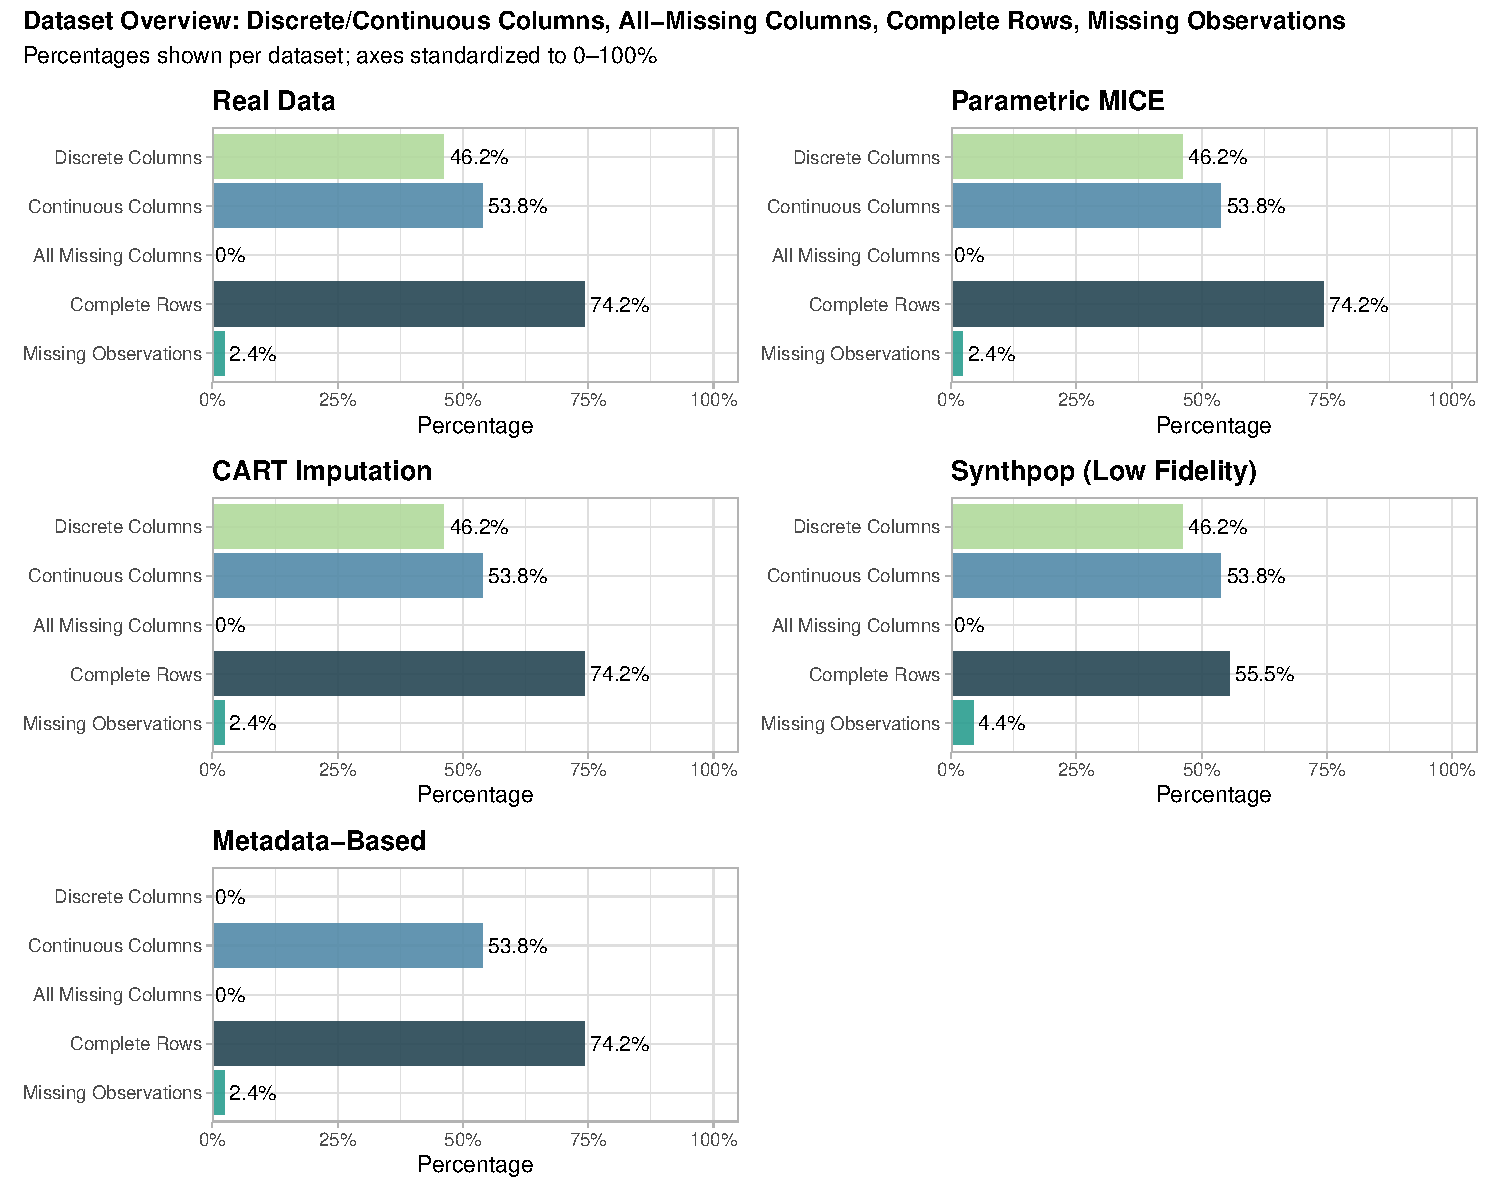
\includegraphics[width=1\linewidth,height=\textheight,keepaspectratio]{heart_failure_synthetic_data_project_files/figure-pdf/intro-plots-1.pdf}
\end{center}

\paragraph{Missingness Proportions and Comparison
Outcome}\label{missingness-proportions-and-comparison-outcome}

\begin{Shaded}
\begin{Highlighting}[]
\CommentTok{\# Helper: remove \textquotesingle{}synth\_\textquotesingle{} prefix so names match the real dataset}
\NormalTok{strip\_synth\_prefix }\OtherTok{\textless{}{-}} \ControlFlowTok{function}\NormalTok{(df) \{}
  \FunctionTok{names}\NormalTok{(df) }\OtherTok{\textless{}{-}} \FunctionTok{sub}\NormalTok{(}\StringTok{"\^{}synth\_"}\NormalTok{, }\StringTok{""}\NormalTok{, }\FunctionTok{names}\NormalTok{(df))}
\NormalTok{  df}
\NormalTok{\}}

\CommentTok{\# Compare against the real dataset\textquotesingle{}s variable set}
\NormalTok{core\_vars }\OtherTok{\textless{}{-}} \FunctionTok{names}\NormalTok{(heart\_failure)}

\CommentTok{\# Function to compute missingness proportions (2 d.p.) for one dataset}
\NormalTok{get\_missingness }\OtherTok{\textless{}{-}} \ControlFlowTok{function}\NormalTok{(df, label) \{}
\NormalTok{  df2 }\OtherTok{\textless{}{-}}\NormalTok{ df }\SpecialCharTok{\%\textgreater{}\%} \FunctionTok{strip\_synth\_prefix}\NormalTok{()}
  \CommentTok{\# keep only variables present in the real data (prevents mismatches)}
\NormalTok{  df2 }\OtherTok{\textless{}{-}}\NormalTok{ df2 }\SpecialCharTok{\%\textgreater{}\%} \FunctionTok{select}\NormalTok{(}\FunctionTok{any\_of}\NormalTok{(core\_vars))}
  \FunctionTok{tibble}\NormalTok{(}
    \AttributeTok{Variable   =} \FunctionTok{names}\NormalTok{(df2),}
    \AttributeTok{Proportion =} \FunctionTok{round}\NormalTok{(}\FunctionTok{colSums}\NormalTok{(}\FunctionTok{is.na}\NormalTok{(df2)) }\SpecialCharTok{/} \FunctionTok{nrow}\NormalTok{(df2), }\DecValTok{2}\NormalTok{),}
    \AttributeTok{Dataset    =}\NormalTok{ label}
\NormalTok{  )}
\NormalTok{\}}

\CommentTok{\# Build tidy table}
\NormalTok{missing\_tbl }\OtherTok{\textless{}{-}} \FunctionTok{bind\_rows}\NormalTok{(}
  \FunctionTok{get\_missingness}\NormalTok{(heart\_failure, }\StringTok{"Real Data"}\NormalTok{),}
  \FunctionTok{get\_missingness}\NormalTok{(syn\_data\_1, }\StringTok{"Parametric MICE"}\NormalTok{),}
  \FunctionTok{get\_missingness}\NormalTok{(syn\_cart\_1, }\StringTok{"CART Imputation"}\NormalTok{),}
  \FunctionTok{get\_missingness}\NormalTok{(syn\_data\_low\_fidelity\_synthpop, }\StringTok{"Synthpop (Low Fidelity)"}\NormalTok{),}
  \FunctionTok{get\_missingness}\NormalTok{(syn\_data\_metadata, }\StringTok{"Metadata{-}Based"}\NormalTok{)}
\NormalTok{)}

\CommentTok{\# Pivot wider for side{-}by{-}side comparison}
\NormalTok{missing\_tbl\_wide }\OtherTok{\textless{}{-}}\NormalTok{ missing\_tbl }\SpecialCharTok{\%\textgreater{}\%}
  \FunctionTok{pivot\_wider}\NormalTok{(}\AttributeTok{names\_from =}\NormalTok{ Dataset, }\AttributeTok{values\_from =}\NormalTok{ Proportion) }\SpecialCharTok{\%\textgreater{}\%}
  \FunctionTok{arrange}\NormalTok{(Variable)}

\CommentTok{\# Optional: add quick match flags (✅ if identical to Real Data)}
\CommentTok{\# missing\_tbl\_wide \textless{}{-} missing\_tbl\_wide \%\textgreater{}\%}
\CommentTok{\#   mutate(}
\CommentTok{\#     \textasciigrave{}Parametric MICE Match\textasciigrave{} = ifelse(\textasciigrave{}Parametric MICE\textasciigrave{} == \textasciigrave{}Real Data\textasciigrave{}, "✅", "❌"),}
\CommentTok{\#     \textasciigrave{}CART Imputation Match\textasciigrave{} = ifelse(\textasciigrave{}CART Imputation\textasciigrave{} == \textasciigrave{}Real Data\textasciigrave{}, "✅", "❌"),}
\CommentTok{\#     \textasciigrave{}Synthpop (Low Fidelity) Match\textasciigrave{} = ifelse(\textasciigrave{}Synthpop (Low Fidelity)\textasciigrave{} == \textasciigrave{}Real Data\textasciigrave{}, "✅", "❌"),}
\CommentTok{\#     \textasciigrave{}Metadata{-}Based Match\textasciigrave{} = ifelse(\textasciigrave{}Metadata{-}Based\textasciigrave{} == \textasciigrave{}Real Data\textasciigrave{}, "✅", "❌")}
\CommentTok{\#   )}

\FunctionTok{kable}\NormalTok{(}
\NormalTok{  missing\_tbl\_wide,}
  \AttributeTok{caption =} \StringTok{"Missingness Proportions by Variable (rounded to 2 d.p.)"}
\NormalTok{)}
\end{Highlighting}
\end{Shaded}

\begin{longtable}[]{@{}
  >{\raggedright\arraybackslash}p{(\linewidth - 10\tabcolsep) * \real{0.2358}}
  >{\raggedleft\arraybackslash}p{(\linewidth - 10\tabcolsep) * \real{0.0943}}
  >{\raggedleft\arraybackslash}p{(\linewidth - 10\tabcolsep) * \real{0.1509}}
  >{\raggedleft\arraybackslash}p{(\linewidth - 10\tabcolsep) * \real{0.1509}}
  >{\raggedleft\arraybackslash}p{(\linewidth - 10\tabcolsep) * \real{0.2264}}
  >{\raggedleft\arraybackslash}p{(\linewidth - 10\tabcolsep) * \real{0.1415}}@{}}
\caption{Missingness Proportions by Variable (rounded to 2
d.p.)}\tabularnewline
\toprule\noalign{}
\begin{minipage}[b]{\linewidth}\raggedright
Variable
\end{minipage} & \begin{minipage}[b]{\linewidth}\raggedleft
Real Data
\end{minipage} & \begin{minipage}[b]{\linewidth}\raggedleft
Parametric MICE
\end{minipage} & \begin{minipage}[b]{\linewidth}\raggedleft
CART Imputation
\end{minipage} & \begin{minipage}[b]{\linewidth}\raggedleft
Synthpop (Low Fidelity)
\end{minipage} & \begin{minipage}[b]{\linewidth}\raggedleft
Metadata-Based
\end{minipage} \\
\midrule\noalign{}
\endfirsthead
\toprule\noalign{}
\begin{minipage}[b]{\linewidth}\raggedright
Variable
\end{minipage} & \begin{minipage}[b]{\linewidth}\raggedleft
Real Data
\end{minipage} & \begin{minipage}[b]{\linewidth}\raggedleft
Parametric MICE
\end{minipage} & \begin{minipage}[b]{\linewidth}\raggedleft
CART Imputation
\end{minipage} & \begin{minipage}[b]{\linewidth}\raggedleft
Synthpop (Low Fidelity)
\end{minipage} & \begin{minipage}[b]{\linewidth}\raggedleft
Metadata-Based
\end{minipage} \\
\midrule\noalign{}
\endhead
\bottomrule\noalign{}
\endlastfoot
age & 0.05 & 0.05 & 0.05 & 0.09 & 0.05 \\
anaemia & 0.00 & 0.00 & 0.00 & 0.00 & 0.00 \\
creatinine\_phosphokinase & 0.05 & 0.05 & 0.05 & 0.10 & 0.05 \\
deceased & 0.00 & 0.00 & 0.00 & 0.00 & 0.00 \\
diabetes & 0.00 & 0.00 & 0.00 & 0.00 & 0.00 \\
ejection\_fraction & 0.04 & 0.04 & 0.04 & 0.05 & 0.04 \\
follow\_up & 0.00 & 0.00 & 0.00 & 0.00 & 0.00 \\
hypertension & 0.00 & 0.00 & 0.00 & 0.00 & 0.00 \\
platelets & 0.05 & 0.05 & 0.05 & 0.10 & 0.05 \\
serum\_creatinine & 0.06 & 0.06 & 0.06 & 0.12 & 0.06 \\
serum\_sodium & 0.07 & 0.07 & 0.07 & 0.11 & 0.07 \\
sex & 0.00 & 0.00 & 0.00 & 0.00 & 0.00 \\
smoking & 0.00 & 0.00 & 0.00 & 0.00 & 0.00 \\
\end{longtable}

\paragraph{Missingness Maps}\label{missingness-maps}

\begin{Shaded}
\begin{Highlighting}[]
\CommentTok{\# Generate missingness map for the real dataset}
\NormalTok{real\_missing\_map }\OtherTok{\textless{}{-}} \FunctionTok{aggr}\NormalTok{(heart\_failure, }\AttributeTok{col =} \FunctionTok{c}\NormalTok{(}\StringTok{"\#B0D99B"}\NormalTok{, }\StringTok{"\#528AA8"}\NormalTok{),}
                             \AttributeTok{numbers =} \ConstantTok{TRUE}\NormalTok{, }\AttributeTok{sortVars =} \ConstantTok{TRUE}\NormalTok{,}
                             \AttributeTok{labels =} \FunctionTok{names}\NormalTok{(heart\_failure), }\AttributeTok{cex.axis =}\NormalTok{ .}\DecValTok{7}\NormalTok{,}
                             \AttributeTok{gap =} \DecValTok{3}\NormalTok{, }\AttributeTok{ylab =} \FunctionTok{c}\NormalTok{(}\StringTok{"Missing Data"}\NormalTok{, }\StringTok{"Pattern {-} real Dataset"}\NormalTok{))}
\end{Highlighting}
\end{Shaded}

\begin{center}
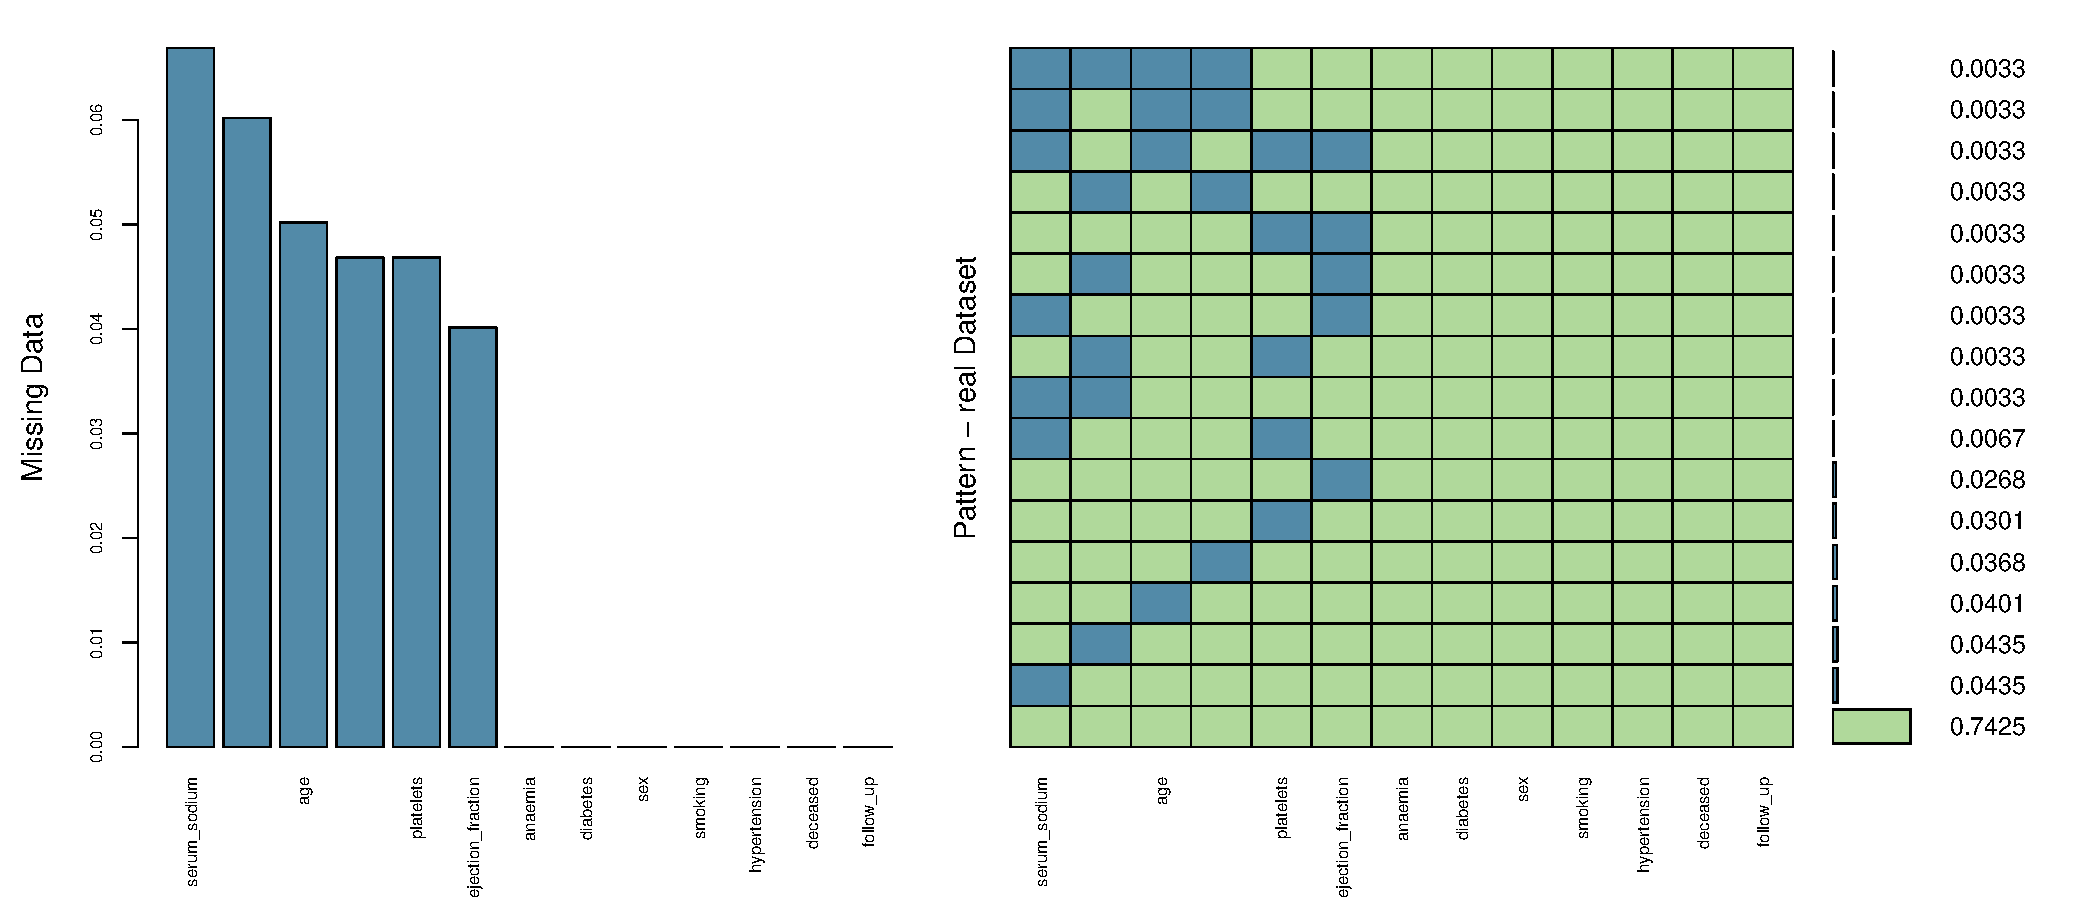
\includegraphics[width=1\linewidth,height=\textheight,keepaspectratio]{heart_failure_synthetic_data_project_files/figure-pdf/Missingness Maps-1.pdf}
\end{center}

\begin{verbatim}

 Variables sorted by number of missings: 
                 Variable      Count
             serum_sodium 0.06688963
         serum_creatinine 0.06020067
                      age 0.05016722
 creatinine_phosphokinase 0.04682274
                platelets 0.04682274
        ejection_fraction 0.04013378
                  anaemia 0.00000000
                 diabetes 0.00000000
                      sex 0.00000000
                  smoking 0.00000000
             hypertension 0.00000000
                 deceased 0.00000000
                follow_up 0.00000000
\end{verbatim}

\begin{Shaded}
\begin{Highlighting}[]
\CommentTok{\# Generate missingness map for Parametric MICE synthetic dataset}
\NormalTok{parametric\_mice\_missing\_map }\OtherTok{\textless{}{-}} \FunctionTok{aggr}\NormalTok{(syn\_data\_1, }\AttributeTok{col =} \FunctionTok{c}\NormalTok{(}\StringTok{"\#B0D99B"}\NormalTok{, }\StringTok{"\#528AA8"}\NormalTok{),}
                                    \AttributeTok{numbers =} \ConstantTok{TRUE}\NormalTok{, }\AttributeTok{sortVars =} \ConstantTok{TRUE}\NormalTok{,}
                                    \AttributeTok{labels =} \FunctionTok{names}\NormalTok{(syn\_data\_1), }\AttributeTok{cex.axis =}\NormalTok{ .}\DecValTok{7}\NormalTok{,}
                                    \AttributeTok{gap =} \DecValTok{3}\NormalTok{, }\AttributeTok{ylab =} \FunctionTok{c}\NormalTok{(}\StringTok{"Missing Data"}\NormalTok{, }\StringTok{"Pattern {-} Parametric MICE Dataset"}\NormalTok{))}
\end{Highlighting}
\end{Shaded}

\begin{center}
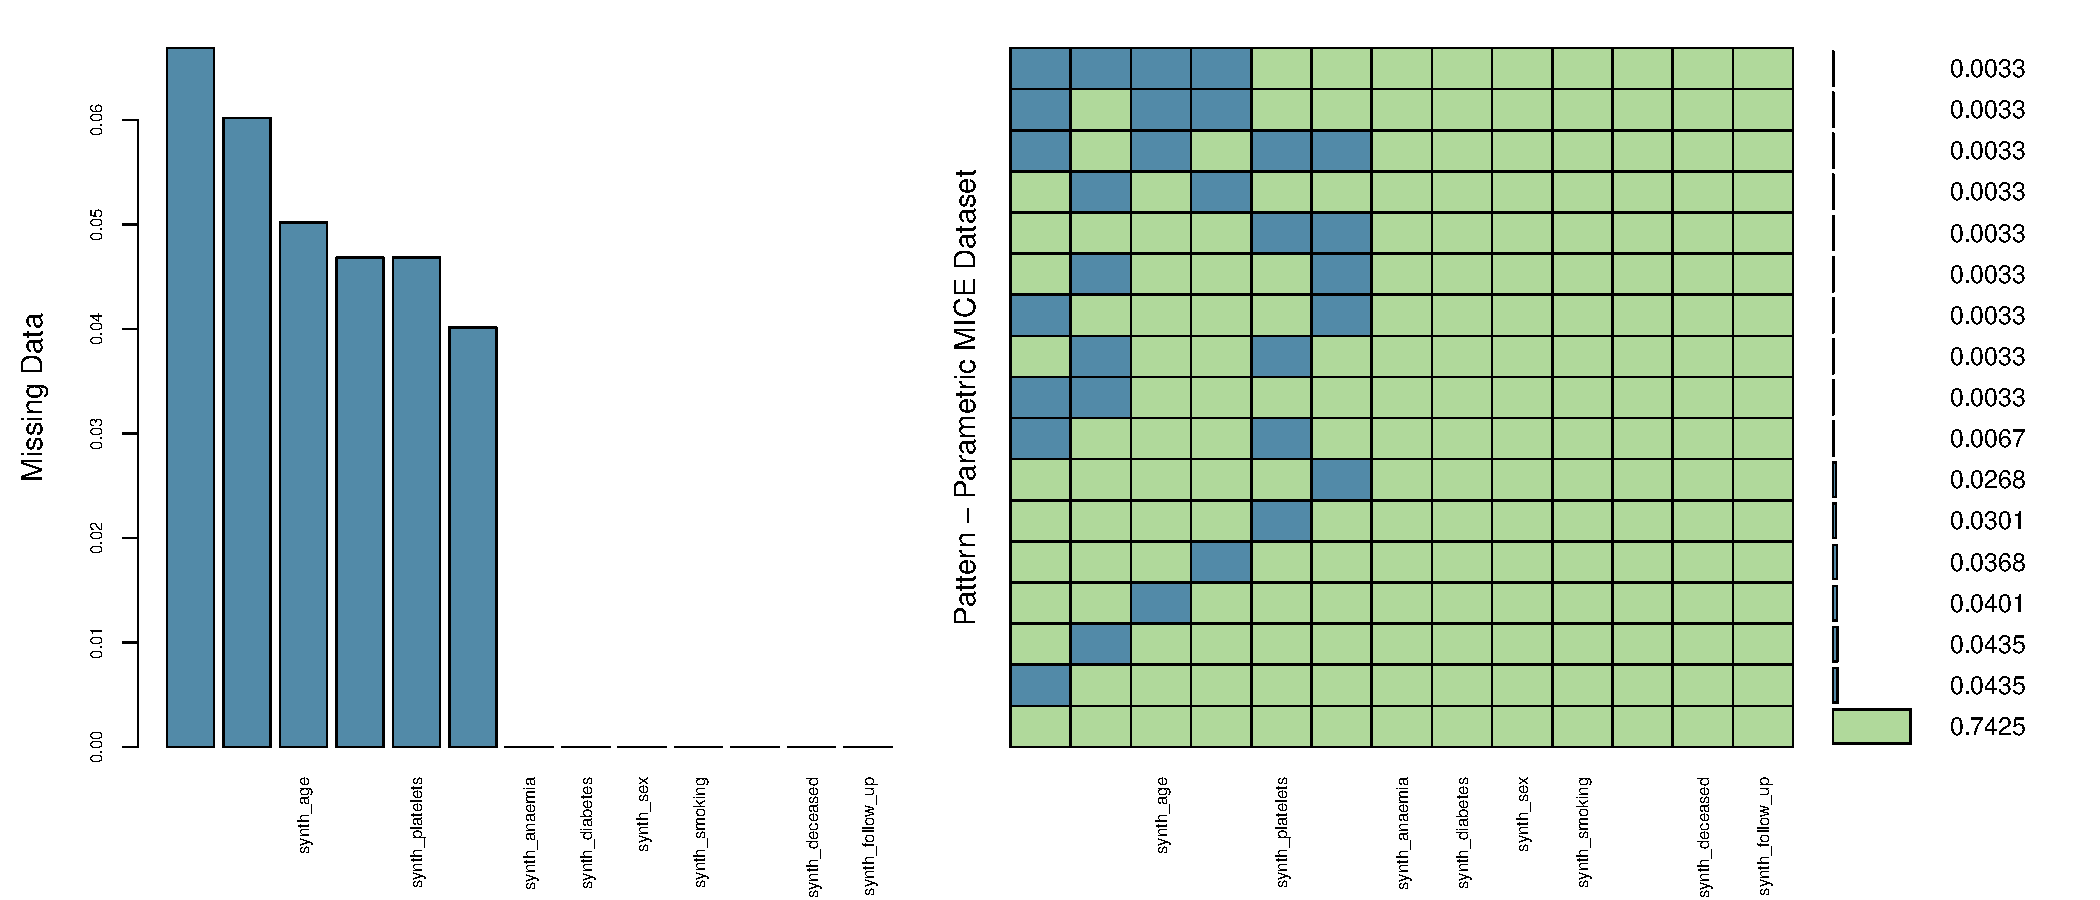
\includegraphics[width=1\linewidth,height=\textheight,keepaspectratio]{heart_failure_synthetic_data_project_files/figure-pdf/Missingness Maps-2.pdf}
\end{center}

\begin{verbatim}

 Variables sorted by number of missings: 
                       Variable      Count
             synth_serum_sodium 0.06688963
         synth_serum_creatinine 0.06020067
                      synth_age 0.05016722
 synth_creatinine_phosphokinase 0.04682274
                synth_platelets 0.04682274
        synth_ejection_fraction 0.04013378
                  synth_anaemia 0.00000000
                 synth_diabetes 0.00000000
                      synth_sex 0.00000000
                  synth_smoking 0.00000000
             synth_hypertension 0.00000000
                 synth_deceased 0.00000000
                synth_follow_up 0.00000000
\end{verbatim}

\begin{Shaded}
\begin{Highlighting}[]
\CommentTok{\# Generate missingness map for CART synthetic dataset}
\NormalTok{cart\_missing\_map }\OtherTok{\textless{}{-}} \FunctionTok{aggr}\NormalTok{(syn\_cart\_1, }\AttributeTok{col =} \FunctionTok{c}\NormalTok{(}\StringTok{"\#B0D99B"}\NormalTok{, }\StringTok{"\#528AA8"}\NormalTok{),}
                         \AttributeTok{numbers =} \ConstantTok{TRUE}\NormalTok{, }\AttributeTok{sortVars =} \ConstantTok{TRUE}\NormalTok{,}
                         \AttributeTok{labels =} \FunctionTok{names}\NormalTok{(syn\_cart\_1), }\AttributeTok{cex.axis =}\NormalTok{ .}\DecValTok{7}\NormalTok{,}
                         \AttributeTok{gap =} \DecValTok{3}\NormalTok{, }\AttributeTok{ylab =} \FunctionTok{c}\NormalTok{(}\StringTok{"Missing Data"}\NormalTok{, }\StringTok{"Pattern {-} CART Dataset"}\NormalTok{))}
\end{Highlighting}
\end{Shaded}

\begin{center}
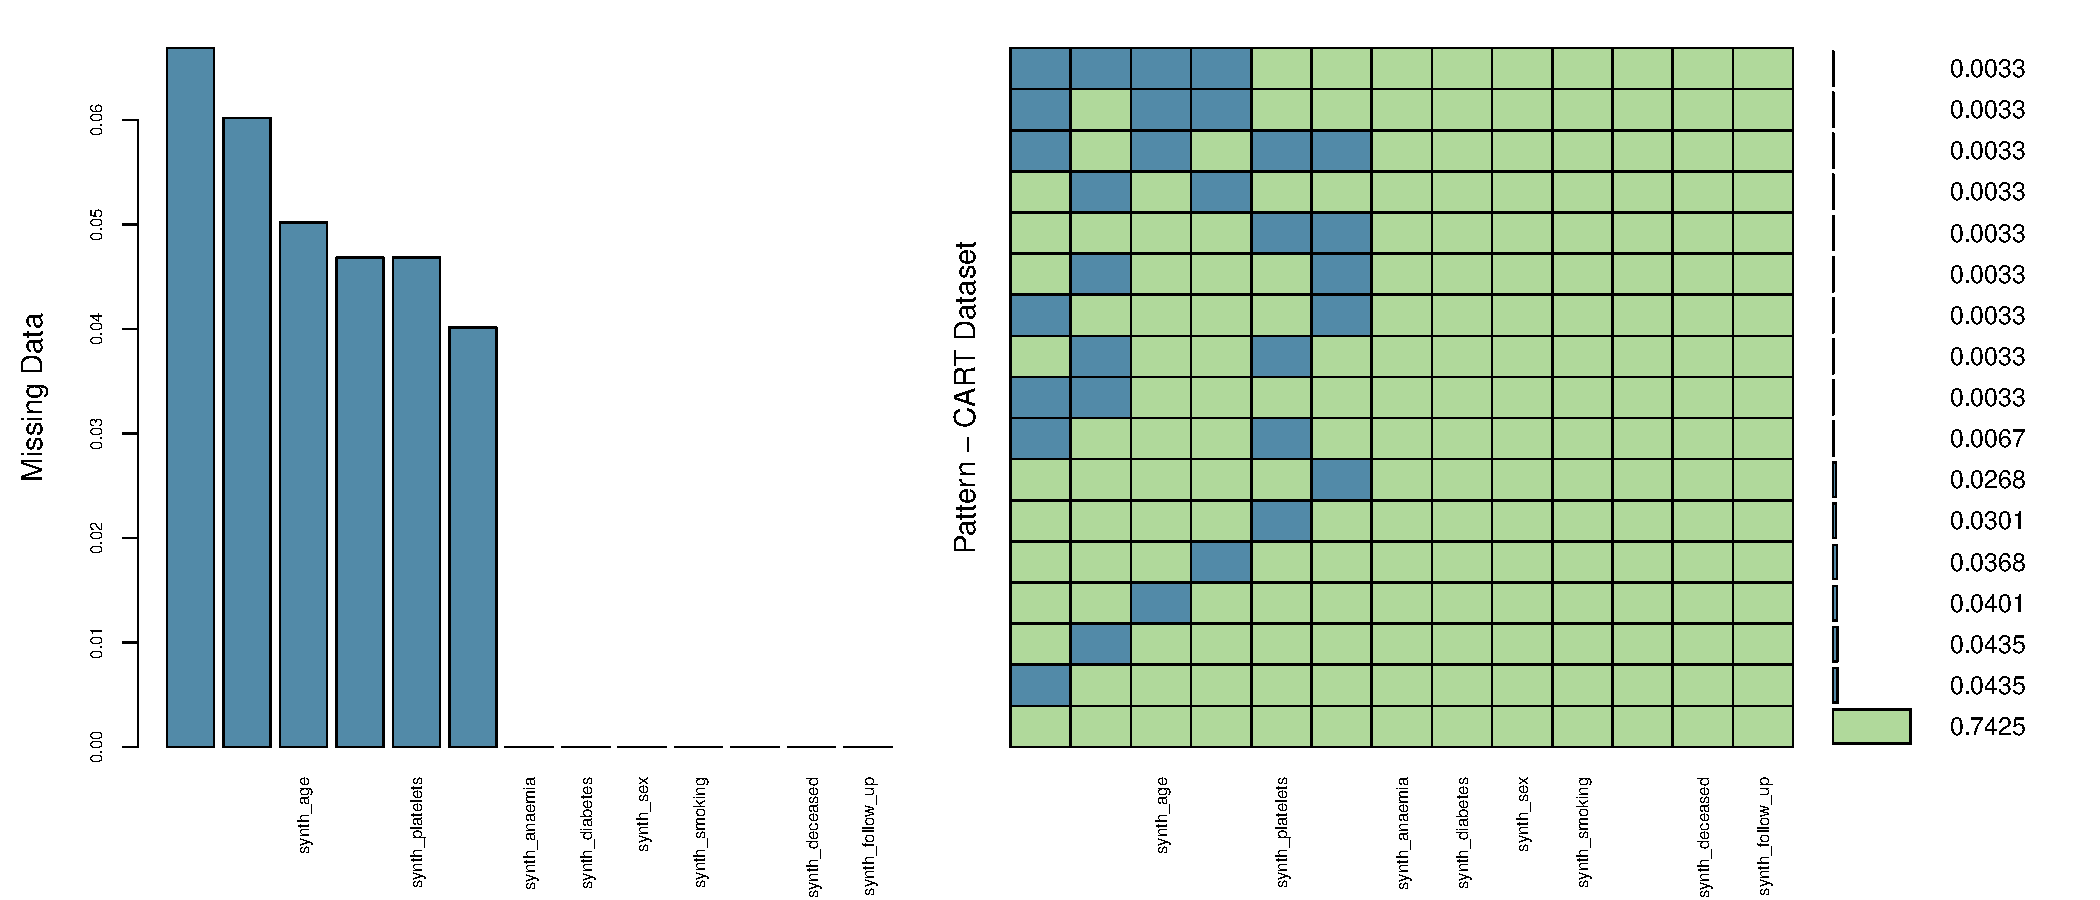
\includegraphics[width=1\linewidth,height=\textheight,keepaspectratio]{heart_failure_synthetic_data_project_files/figure-pdf/Missingness Maps-3.pdf}
\end{center}

\begin{verbatim}

 Variables sorted by number of missings: 
                       Variable      Count
             synth_serum_sodium 0.06688963
         synth_serum_creatinine 0.06020067
                      synth_age 0.05016722
 synth_creatinine_phosphokinase 0.04682274
                synth_platelets 0.04682274
        synth_ejection_fraction 0.04013378
                  synth_anaemia 0.00000000
                 synth_diabetes 0.00000000
                      synth_sex 0.00000000
                  synth_smoking 0.00000000
             synth_hypertension 0.00000000
                 synth_deceased 0.00000000
                synth_follow_up 0.00000000
\end{verbatim}

\begin{Shaded}
\begin{Highlighting}[]
\CommentTok{\# Generate missingness map for Synthpop synthetic dataset}
\NormalTok{synthpop\_missing\_map }\OtherTok{\textless{}{-}} \FunctionTok{aggr}\NormalTok{(syn\_data\_low\_fidelity\_synthpop, }\AttributeTok{col =} \FunctionTok{c}\NormalTok{(}\StringTok{"\#B0D99B"}\NormalTok{, }\StringTok{"\#528AA8"}\NormalTok{),}
                             \AttributeTok{numbers =} \ConstantTok{TRUE}\NormalTok{, }\AttributeTok{sortVars =} \ConstantTok{TRUE}\NormalTok{,}
                             \AttributeTok{labels =} \FunctionTok{names}\NormalTok{(syn\_data\_low\_fidelity\_synthpop), }\AttributeTok{cex.axis =}\NormalTok{ .}\DecValTok{7}\NormalTok{,}
                             \AttributeTok{gap =} \DecValTok{3}\NormalTok{, }\AttributeTok{ylab =} \FunctionTok{c}\NormalTok{(}\StringTok{"Missing Data"}\NormalTok{, }\StringTok{"Pattern {-} Synthpop Dataset"}\NormalTok{))}
\end{Highlighting}
\end{Shaded}

\begin{center}
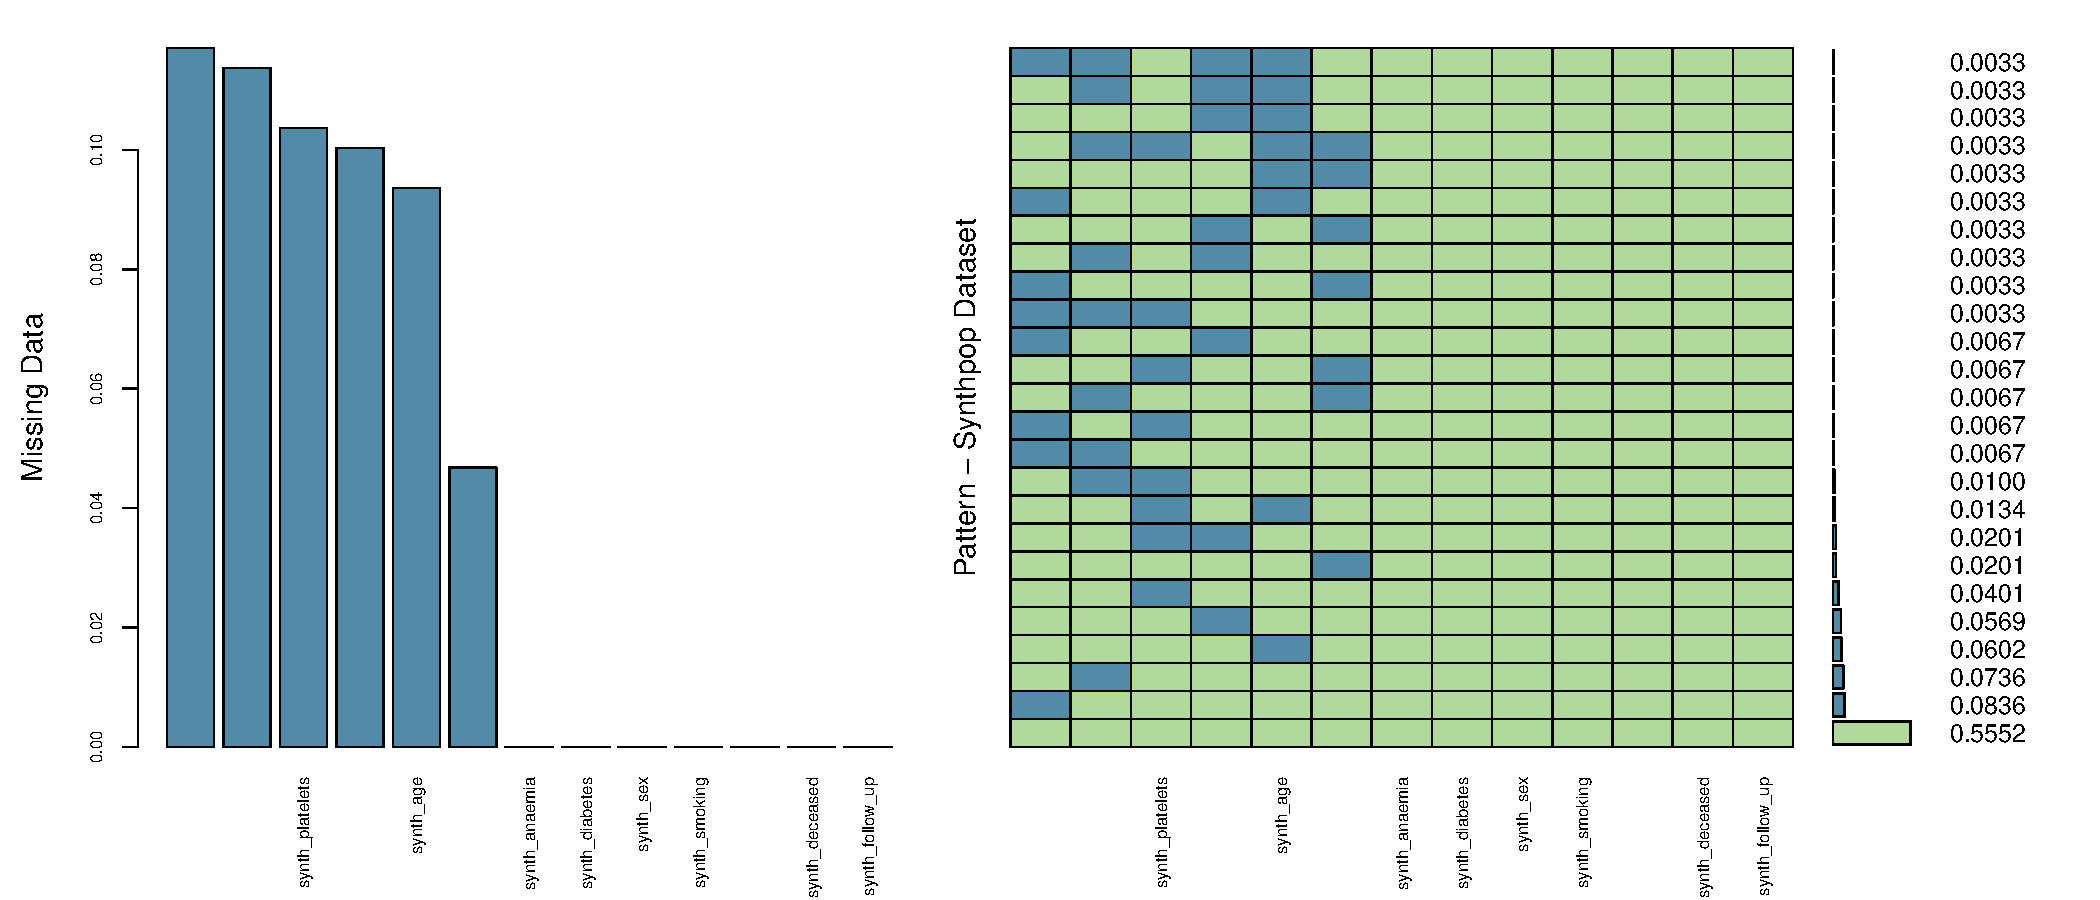
\includegraphics[width=1\linewidth,height=\textheight,keepaspectratio]{heart_failure_synthetic_data_project_files/figure-pdf/Missingness Maps-4.pdf}
\end{center}

\begin{verbatim}

 Variables sorted by number of missings: 
                       Variable      Count
         synth_serum_creatinine 0.11705686
             synth_serum_sodium 0.11371237
                synth_platelets 0.10367893
 synth_creatinine_phosphokinase 0.10033445
                      synth_age 0.09364548
        synth_ejection_fraction 0.04682274
                  synth_anaemia 0.00000000
                 synth_diabetes 0.00000000
                      synth_sex 0.00000000
                  synth_smoking 0.00000000
             synth_hypertension 0.00000000
                 synth_deceased 0.00000000
                synth_follow_up 0.00000000
\end{verbatim}

\begin{Shaded}
\begin{Highlighting}[]
\CommentTok{\# Generate missingness map for Metadata{-}based synthetic dataset}
\NormalTok{metadata\_missing\_map }\OtherTok{\textless{}{-}} \FunctionTok{aggr}\NormalTok{(syn\_data\_metadata, }\AttributeTok{col =} \FunctionTok{c}\NormalTok{(}\StringTok{"\#B0D99B"}\NormalTok{, }\StringTok{"\#528AA8"}\NormalTok{),}
                             \AttributeTok{numbers =} \ConstantTok{TRUE}\NormalTok{, }\AttributeTok{sortVars =} \ConstantTok{TRUE}\NormalTok{,}
                             \AttributeTok{labels =} \FunctionTok{names}\NormalTok{(syn\_data\_metadata), }\AttributeTok{cex.axis =}\NormalTok{ .}\DecValTok{7}\NormalTok{,}
                             \AttributeTok{gap =} \DecValTok{3}\NormalTok{, }\AttributeTok{ylab =} \FunctionTok{c}\NormalTok{(}\StringTok{"Missing Data"}\NormalTok{, }\StringTok{"Pattern {-} Metadata{-}Based Dataset"}\NormalTok{))}
\end{Highlighting}
\end{Shaded}

\begin{center}
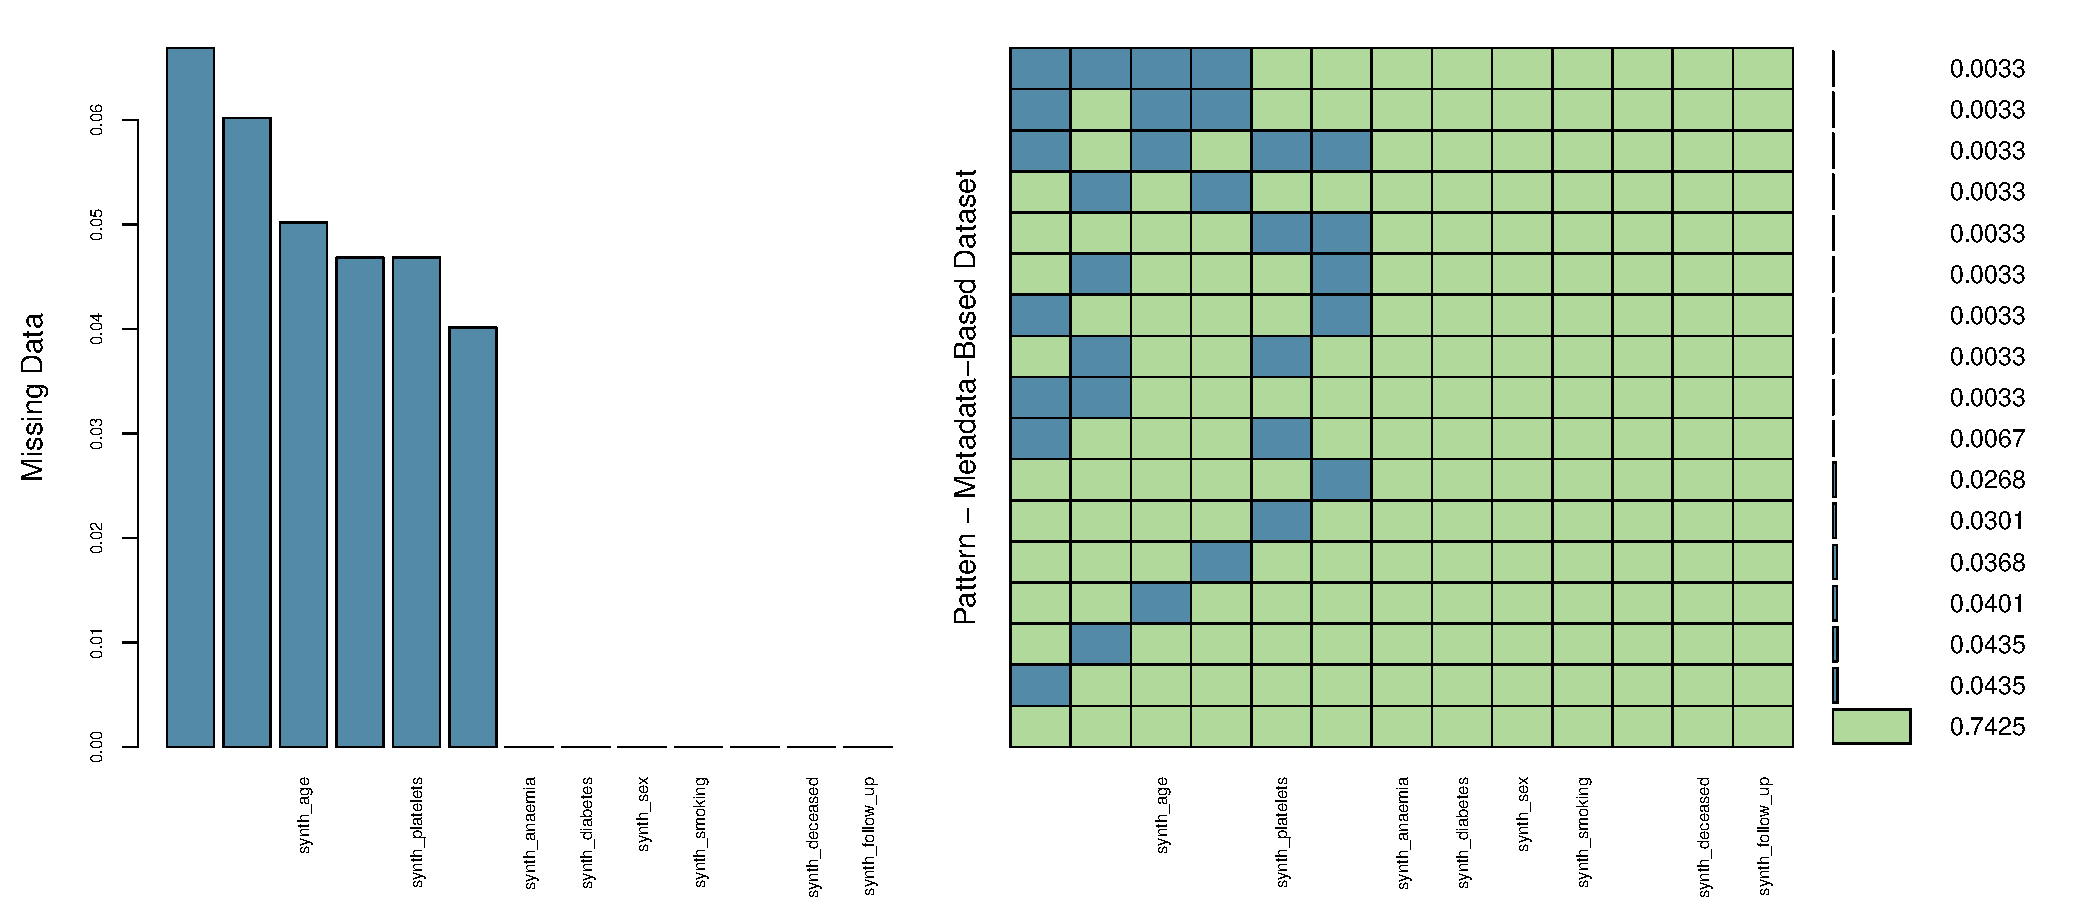
\includegraphics[width=1\linewidth,height=\textheight,keepaspectratio]{heart_failure_synthetic_data_project_files/figure-pdf/Missingness Maps-5.pdf}
\end{center}

\begin{verbatim}

 Variables sorted by number of missings: 
                       Variable      Count
             synth_serum_sodium 0.06688963
         synth_serum_creatinine 0.06020067
                      synth_age 0.05016722
 synth_creatinine_phosphokinase 0.04682274
                synth_platelets 0.04682274
        synth_ejection_fraction 0.04013378
                  synth_anaemia 0.00000000
                 synth_diabetes 0.00000000
                      synth_sex 0.00000000
                  synth_smoking 0.00000000
             synth_hypertension 0.00000000
                 synth_deceased 0.00000000
                synth_follow_up 0.00000000
\end{verbatim}

\subsubsection{Correlation Matrices
Comparison}\label{correlation-matrices-comparison}

In this section, we assess how well the correlations between numeric
variables are preserved in the synthetic datasets compared to the real
dataset. By comparing the correlation matrices, we evaluate whether the
relationships between variables in the real data are reflected in the
synthetic versions. This assessment is essential because maintaining the
real data's correlation structure ensures that any statistical or
machine learning models trained on synthetic data will behave similarly
to those trained on real data.

\begin{itemize}
\item
  \textbf{Correlation Matrix}: A correlation matrix quantifies the
  strength and direction of relationships between pairs of numeric
  variables. Each cell in the matrix represents the correlation
  coefficient between two variables, which can range from -1 (perfect
  negative correlation) to +1 (perfect positive correlation). It is
  crucial that synthetic data retains these relationships to ensure that
  any analyses based on these dependencies remain valid.
\item
  \textbf{Comparison Process}: The correlation matrices for both the
  real and synthetic datasets are computed and Visualised. Ideally, the
  structure and strength of correlations in the synthetic datasets
  should closely match those in the real dataset. Differences in
  correlation strength or direction indicate that the synthetic data may
  not fully capture the underlying relationships, which can affect the
  validity of any conclusions drawn from analyses using the synthetic
  data.
\end{itemize}

Maintaining similar correlation structures is particularly important for
use cases where relationships between variables play a crucial role,
such as in predictive modeling, feature selection, and understanding
variable dependencies. The following sections outline different methods
used to compare correlation matrices between the real and synthetic
datasets.

\paragraph{Correlation Matrices Comparison using
psych}\label{correlation-matrices-comparison-using-psych}

The \texttt{psych} package provides tools for analyzing and visualizing
correlation matrices. The \texttt{corr.test()} function is particularly
useful for computing correlation coefficients while handling missing
data and providing additional statistics, such as confidence intervals.

\begin{Shaded}
\begin{Highlighting}[]
\CommentTok{\# Helper: strip \textquotesingle{}synth\_\textquotesingle{} so names line up with real}
\NormalTok{strip\_synth\_prefix }\OtherTok{\textless{}{-}} \ControlFlowTok{function}\NormalTok{(df) \{}
  \FunctionTok{names}\NormalTok{(df) }\OtherTok{\textless{}{-}} \FunctionTok{sub}\NormalTok{(}\StringTok{"\^{}synth\_"}\NormalTok{, }\StringTok{""}\NormalTok{, }\FunctionTok{names}\NormalTok{(df))}
\NormalTok{  df}
\NormalTok{\}}

\CommentTok{\# Build a tidy table of pairwise correlations for real vs one synthetic dataset}
\NormalTok{corr\_compare\_one }\OtherTok{\textless{}{-}} \ControlFlowTok{function}\NormalTok{(real, synth, label) \{}
\NormalTok{  real\_num  }\OtherTok{\textless{}{-}}\NormalTok{ real }\SpecialCharTok{|\textgreater{}} \FunctionTok{select}\NormalTok{(}\FunctionTok{where}\NormalTok{(is.numeric))}
\NormalTok{  synth\_num }\OtherTok{\textless{}{-}}\NormalTok{ synth }\SpecialCharTok{|\textgreater{}} \FunctionTok{strip\_synth\_prefix}\NormalTok{() }\SpecialCharTok{|\textgreater{}} \FunctionTok{select}\NormalTok{(}\FunctionTok{where}\NormalTok{(is.numeric))}

\NormalTok{  common }\OtherTok{\textless{}{-}} \FunctionTok{intersect}\NormalTok{(}\FunctionTok{names}\NormalTok{(real\_num), }\FunctionTok{names}\NormalTok{(synth\_num))}
  \ControlFlowTok{if}\NormalTok{ (}\FunctionTok{length}\NormalTok{(common) }\SpecialCharTok{\textless{}} \DecValTok{2}\NormalTok{) \{}
    \FunctionTok{return}\NormalTok{(}\FunctionTok{tibble}\NormalTok{(}\AttributeTok{Dataset =}\NormalTok{ label, }\AttributeTok{Var1 =} \FunctionTok{character}\NormalTok{(), }\AttributeTok{Var2 =} \FunctionTok{character}\NormalTok{(),}
                  \AttributeTok{Real =} \FunctionTok{numeric}\NormalTok{(), }\AttributeTok{Synthetic =} \FunctionTok{numeric}\NormalTok{(), }\AttributeTok{Diff =} \FunctionTok{numeric}\NormalTok{(), }\AttributeTok{AbsDiff =} \FunctionTok{numeric}\NormalTok{()))}
\NormalTok{  \}}

  \CommentTok{\# Compute Pearson correlations with pairwise complete observations}
\NormalTok{  rc }\OtherTok{\textless{}{-}} \FunctionTok{cor}\NormalTok{(real\_num[common],  }\AttributeTok{use =} \StringTok{"pairwise.complete.obs"}\NormalTok{, }\AttributeTok{method =} \StringTok{"pearson"}\NormalTok{)}
\NormalTok{  sc }\OtherTok{\textless{}{-}} \FunctionTok{cor}\NormalTok{(synth\_num[common], }\AttributeTok{use =} \StringTok{"pairwise.complete.obs"}\NormalTok{, }\AttributeTok{method =} \StringTok{"pearson"}\NormalTok{)}

  \CommentTok{\# Keep only upper triangle (unique pairs)}
\NormalTok{  ut }\OtherTok{\textless{}{-}} \FunctionTok{upper.tri}\NormalTok{(rc, }\AttributeTok{diag =} \ConstantTok{FALSE}\NormalTok{)}
\NormalTok{  pairs }\OtherTok{\textless{}{-}} \FunctionTok{which}\NormalTok{(ut, }\AttributeTok{arr.ind =} \ConstantTok{TRUE}\NormalTok{)}
  \FunctionTok{tibble}\NormalTok{(}
    \AttributeTok{Var1 =} \FunctionTok{colnames}\NormalTok{(rc)[pairs[, }\DecValTok{1}\NormalTok{]],}
    \AttributeTok{Var2 =} \FunctionTok{colnames}\NormalTok{(rc)[pairs[, }\DecValTok{2}\NormalTok{]],}
    \AttributeTok{Real =}\NormalTok{ rc[pairs],}
    \AttributeTok{Synthetic =}\NormalTok{ sc[pairs]}
\NormalTok{  ) }\SpecialCharTok{|\textgreater{}}
    \FunctionTok{mutate}\NormalTok{(}
      \AttributeTok{Dataset =}\NormalTok{ label,}
      \AttributeTok{Diff =}\NormalTok{ Synthetic }\SpecialCharTok{{-}}\NormalTok{ Real,}
      \AttributeTok{AbsDiff =} \FunctionTok{abs}\NormalTok{(Diff)}
\NormalTok{    ) }\SpecialCharTok{|\textgreater{}}
    \FunctionTok{select}\NormalTok{(Dataset, Var1, Var2, Real, Synthetic, Diff, AbsDiff)}
\NormalTok{\}}

\CommentTok{\# Build one combined table for all synthetic datasets}
\NormalTok{corr\_cmp\_tbl }\OtherTok{\textless{}{-}} \FunctionTok{bind\_rows}\NormalTok{(}
  \FunctionTok{corr\_compare\_one}\NormalTok{(heart\_failure, syn\_data\_1, }\StringTok{"Parametric MICE"}\NormalTok{),}
  \FunctionTok{corr\_compare\_one}\NormalTok{(heart\_failure, syn\_cart\_1, }\StringTok{"CART Imputation"}\NormalTok{),}
  \FunctionTok{corr\_compare\_one}\NormalTok{(heart\_failure, syn\_data\_low\_fidelity\_synthpop, }\StringTok{"Synthpop (Low Fidelity)"}\NormalTok{),}
  \FunctionTok{corr\_compare\_one}\NormalTok{(heart\_failure, syn\_data\_metadata, }\StringTok{"Metadata{-}Based"}\NormalTok{)}
\NormalTok{) }\SpecialCharTok{|\textgreater{}}
  \FunctionTok{arrange}\NormalTok{(Dataset, }\FunctionTok{desc}\NormalTok{(AbsDiff)) }\SpecialCharTok{|\textgreater{}}
  \FunctionTok{mutate}\NormalTok{(}
    \AttributeTok{Real =} \FunctionTok{round}\NormalTok{(Real, }\DecValTok{2}\NormalTok{),}
    \AttributeTok{Synthetic =} \FunctionTok{round}\NormalTok{(Synthetic, }\DecValTok{2}\NormalTok{),}
    \AttributeTok{Diff =} \FunctionTok{round}\NormalTok{(Diff, }\DecValTok{2}\NormalTok{),}
    \AttributeTok{AbsDiff =} \FunctionTok{round}\NormalTok{(AbsDiff, }\DecValTok{2}\NormalTok{)}
\NormalTok{  )}

\NormalTok{knitr}\SpecialCharTok{::}\FunctionTok{kable}\NormalTok{(}
\NormalTok{  corr\_cmp\_tbl,}
  \AttributeTok{caption =} \StringTok{"Pairwise Correlations: Real vs. Synthetic (sorted by largest absolute difference per dataset)"}\NormalTok{,}
  \AttributeTok{align =} \StringTok{"lllrrrr"}
\NormalTok{)}
\end{Highlighting}
\end{Shaded}

\begin{longtable}[]{@{}
  >{\raggedright\arraybackslash}p{(\linewidth - 12\tabcolsep) * \real{0.2308}}
  >{\raggedright\arraybackslash}p{(\linewidth - 12\tabcolsep) * \real{0.2404}}
  >{\raggedright\arraybackslash}p{(\linewidth - 12\tabcolsep) * \real{0.2404}}
  >{\raggedleft\arraybackslash}p{(\linewidth - 12\tabcolsep) * \real{0.0577}}
  >{\raggedleft\arraybackslash}p{(\linewidth - 12\tabcolsep) * \real{0.0962}}
  >{\raggedleft\arraybackslash}p{(\linewidth - 12\tabcolsep) * \real{0.0577}}
  >{\raggedleft\arraybackslash}p{(\linewidth - 12\tabcolsep) * \real{0.0769}}@{}}
\caption{Pairwise Correlations: Real vs.~Synthetic (sorted by largest
absolute difference per dataset)}\tabularnewline
\toprule\noalign{}
\begin{minipage}[b]{\linewidth}\raggedright
Dataset
\end{minipage} & \begin{minipage}[b]{\linewidth}\raggedright
Var1
\end{minipage} & \begin{minipage}[b]{\linewidth}\raggedright
Var2
\end{minipage} & \begin{minipage}[b]{\linewidth}\raggedleft
Real
\end{minipage} & \begin{minipage}[b]{\linewidth}\raggedleft
Synthetic
\end{minipage} & \begin{minipage}[b]{\linewidth}\raggedleft
Diff
\end{minipage} & \begin{minipage}[b]{\linewidth}\raggedleft
AbsDiff
\end{minipage} \\
\midrule\noalign{}
\endfirsthead
\toprule\noalign{}
\begin{minipage}[b]{\linewidth}\raggedright
Dataset
\end{minipage} & \begin{minipage}[b]{\linewidth}\raggedright
Var1
\end{minipage} & \begin{minipage}[b]{\linewidth}\raggedright
Var2
\end{minipage} & \begin{minipage}[b]{\linewidth}\raggedleft
Real
\end{minipage} & \begin{minipage}[b]{\linewidth}\raggedleft
Synthetic
\end{minipage} & \begin{minipage}[b]{\linewidth}\raggedleft
Diff
\end{minipage} & \begin{minipage}[b]{\linewidth}\raggedleft
AbsDiff
\end{minipage} \\
\midrule\noalign{}
\endhead
\bottomrule\noalign{}
\endlastfoot
CART Imputation & creatinine\_phosphokinase & platelets & 0.01 & -0.12 &
-0.13 & 0.13 \\
CART Imputation & ejection\_fraction & serum\_creatinine & -0.01 & -0.11
& -0.10 & 0.10 \\
CART Imputation & creatinine\_phosphokinase & serum\_sodium & 0.06 &
-0.04 & -0.10 & 0.10 \\
CART Imputation & age & follow\_up & -0.24 & -0.15 & 0.09 & 0.09 \\
CART Imputation & ejection\_fraction & platelets & 0.06 & -0.02 & -0.08
& 0.08 \\
CART Imputation & age & serum\_creatinine & 0.17 & 0.25 & 0.08 & 0.08 \\
CART Imputation & platelets & serum\_creatinine & -0.05 & 0.03 & 0.08 &
0.08 \\
CART Imputation & ejection\_fraction & follow\_up & 0.03 & -0.05 & -0.08
& 0.08 \\
CART Imputation & serum\_sodium & follow\_up & 0.11 & 0.03 & -0.07 &
0.07 \\
CART Imputation & age & creatinine\_phosphokinase & -0.08 & -0.15 &
-0.07 & 0.07 \\
CART Imputation & platelets & serum\_sodium & 0.06 & -0.01 & -0.07 &
0.07 \\
CART Imputation & creatinine\_phosphokinase & follow\_up & -0.03 & 0.03
& 0.06 & 0.06 \\
CART Imputation & platelets & follow\_up & -0.01 & 0.05 & 0.06 & 0.06 \\
CART Imputation & age & platelets & -0.05 & -0.01 & 0.04 & 0.04 \\
CART Imputation & age & serum\_sodium & -0.04 & -0.08 & -0.04 & 0.04 \\
CART Imputation & age & ejection\_fraction & 0.04 & 0.00 & -0.04 &
0.04 \\
CART Imputation & creatinine\_phosphokinase & ejection\_fraction & -0.05
& -0.02 & 0.03 & 0.03 \\
CART Imputation & creatinine\_phosphokinase & serum\_creatinine & 0.00 &
-0.02 & -0.02 & 0.02 \\
CART Imputation & serum\_creatinine & serum\_sodium & -0.21 & -0.23 &
-0.02 & 0.02 \\
CART Imputation & ejection\_fraction & serum\_sodium & 0.17 & 0.18 &
0.02 & 0.02 \\
CART Imputation & serum\_creatinine & follow\_up & -0.15 & -0.14 & 0.01
& 0.01 \\
Metadata-Based & age & follow\_up & -0.24 & 0.12 & 0.36 & 0.36 \\
Metadata-Based & platelets & serum\_sodium & 0.06 & -0.16 & -0.23 &
0.23 \\
Metadata-Based & serum\_creatinine & serum\_sodium & -0.21 & 0.01 & 0.21
& 0.21 \\
Metadata-Based & creatinine\_phosphokinase & ejection\_fraction & -0.05
& 0.11 & 0.16 & 0.16 \\
Metadata-Based & ejection\_fraction & serum\_sodium & 0.17 & 0.03 &
-0.13 & 0.13 \\
Metadata-Based & creatinine\_phosphokinase & serum\_creatinine & 0.00 &
-0.12 & -0.13 & 0.13 \\
Metadata-Based & creatinine\_phosphokinase & follow\_up & -0.03 & 0.09 &
0.12 & 0.12 \\
Metadata-Based & age & serum\_creatinine & 0.17 & 0.07 & -0.10 & 0.10 \\
Metadata-Based & serum\_sodium & follow\_up & 0.11 & 0.00 & -0.10 &
0.10 \\
Metadata-Based & age & serum\_sodium & -0.04 & 0.06 & 0.10 & 0.10 \\
Metadata-Based & serum\_creatinine & follow\_up & -0.15 & -0.05 & 0.09 &
0.09 \\
Metadata-Based & creatinine\_phosphokinase & platelets & 0.01 & -0.08 &
-0.09 & 0.09 \\
Metadata-Based & ejection\_fraction & platelets & 0.06 & -0.02 & -0.08 &
0.08 \\
Metadata-Based & age & platelets & -0.05 & 0.02 & 0.07 & 0.07 \\
Metadata-Based & age & ejection\_fraction & 0.04 & -0.03 & -0.07 &
0.07 \\
Metadata-Based & ejection\_fraction & follow\_up & 0.03 & 0.08 & 0.05 &
0.05 \\
Metadata-Based & creatinine\_phosphokinase & serum\_sodium & 0.06 & 0.11
& 0.05 & 0.05 \\
Metadata-Based & age & creatinine\_phosphokinase & -0.08 & -0.05 & 0.03
& 0.03 \\
Metadata-Based & ejection\_fraction & serum\_creatinine & -0.01 & 0.01 &
0.02 & 0.02 \\
Metadata-Based & platelets & follow\_up & -0.01 & -0.02 & -0.01 &
0.01 \\
Metadata-Based & platelets & serum\_creatinine & -0.05 & -0.06 & -0.01 &
0.01 \\
Parametric MICE & serum\_creatinine & serum\_sodium & -0.21 & 0.02 &
0.23 & 0.23 \\
Parametric MICE & ejection\_fraction & follow\_up & 0.03 & 0.20 & 0.17 &
0.17 \\
Parametric MICE & age & follow\_up & -0.24 & -0.08 & 0.16 & 0.16 \\
Parametric MICE & ejection\_fraction & serum\_sodium & 0.17 & 0.03 &
-0.13 & 0.13 \\
Parametric MICE & serum\_sodium & follow\_up & 0.11 & -0.01 & -0.11 &
0.11 \\
Parametric MICE & platelets & serum\_creatinine & -0.05 & 0.06 & 0.11 &
0.11 \\
Parametric MICE & creatinine\_phosphokinase & serum\_creatinine & 0.00 &
-0.11 & -0.11 & 0.11 \\
Parametric MICE & age & serum\_creatinine & 0.17 & 0.08 & -0.09 &
0.09 \\
Parametric MICE & creatinine\_phosphokinase & platelets & 0.01 & -0.07 &
-0.08 & 0.08 \\
Parametric MICE & age & serum\_sodium & -0.04 & -0.11 & -0.07 & 0.07 \\
Parametric MICE & age & creatinine\_phosphokinase & -0.08 & -0.02 & 0.06
& 0.06 \\
Parametric MICE & creatinine\_phosphokinase & follow\_up & -0.03 & 0.03
& 0.06 & 0.06 \\
Parametric MICE & platelets & follow\_up & -0.01 & 0.04 & 0.05 & 0.05 \\
Parametric MICE & creatinine\_phosphokinase & ejection\_fraction & -0.05
& -0.01 & 0.04 & 0.04 \\
Parametric MICE & serum\_creatinine & follow\_up & -0.15 & -0.11 & 0.04
& 0.04 \\
Parametric MICE & platelets & serum\_sodium & 0.06 & 0.03 & -0.03 &
0.03 \\
Parametric MICE & creatinine\_phosphokinase & serum\_sodium & 0.06 &
0.03 & -0.03 & 0.03 \\
Parametric MICE & ejection\_fraction & serum\_creatinine & -0.01 & -0.04
& -0.03 & 0.03 \\
Parametric MICE & age & platelets & -0.05 & -0.03 & 0.02 & 0.02 \\
Parametric MICE & age & ejection\_fraction & 0.04 & 0.05 & 0.01 &
0.01 \\
Parametric MICE & ejection\_fraction & platelets & 0.06 & 0.06 & 0.00 &
0.00 \\
Synthpop (Low Fidelity) & age & follow\_up & -0.24 & 0.04 & 0.28 &
0.28 \\
Synthpop (Low Fidelity) & serum\_creatinine & serum\_sodium & -0.21 &
0.00 & 0.20 & 0.20 \\
Synthpop (Low Fidelity) & age & serum\_creatinine & 0.17 & -0.03 & -0.20
& 0.20 \\
Synthpop (Low Fidelity) & ejection\_fraction & serum\_sodium & 0.17 &
-0.02 & -0.19 & 0.19 \\
Synthpop (Low Fidelity) & age & serum\_sodium & -0.04 & 0.11 & 0.15 &
0.15 \\
Synthpop (Low Fidelity) & serum\_creatinine & follow\_up & -0.15 & 0.00
& 0.15 & 0.15 \\
Synthpop (Low Fidelity) & serum\_sodium & follow\_up & 0.11 & -0.03 &
-0.14 & 0.14 \\
Synthpop (Low Fidelity) & age & creatinine\_phosphokinase & -0.08 & 0.03
& 0.12 & 0.12 \\
Synthpop (Low Fidelity) & creatinine\_phosphokinase & ejection\_fraction
& -0.05 & 0.05 & 0.10 & 0.10 \\
Synthpop (Low Fidelity) & ejection\_fraction & platelets & 0.06 & 0.15 &
0.09 & 0.09 \\
Synthpop (Low Fidelity) & platelets & follow\_up & -0.01 & 0.08 & 0.09 &
0.09 \\
Synthpop (Low Fidelity) & ejection\_fraction & follow\_up & 0.03 & 0.09
& 0.06 & 0.06 \\
Synthpop (Low Fidelity) & creatinine\_phosphokinase & platelets & 0.01 &
-0.05 & -0.06 & 0.06 \\
Synthpop (Low Fidelity) & age & ejection\_fraction & 0.04 & -0.02 &
-0.06 & 0.06 \\
Synthpop (Low Fidelity) & ejection\_fraction & serum\_creatinine & -0.01
& -0.06 & -0.05 & 0.05 \\
Synthpop (Low Fidelity) & creatinine\_phosphokinase & serum\_sodium &
0.06 & 0.01 & -0.05 & 0.05 \\
Synthpop (Low Fidelity) & creatinine\_phosphokinase & follow\_up & -0.03
& 0.02 & 0.04 & 0.04 \\
Synthpop (Low Fidelity) & platelets & serum\_creatinine & -0.05 & -0.08
& -0.03 & 0.03 \\
Synthpop (Low Fidelity) & creatinine\_phosphokinase & serum\_creatinine
& 0.00 & -0.02 & -0.03 & 0.03 \\
Synthpop (Low Fidelity) & platelets & serum\_sodium & 0.06 & 0.08 & 0.02
& 0.02 \\
Synthpop (Low Fidelity) & age & platelets & -0.05 & -0.04 & 0.01 &
0.01 \\
\end{longtable}

\paragraph{Correlation Matrices Comparison using
Corrplot}\label{correlation-matrices-comparison-using-corrplot}

The \texttt{corrplot} package is widely used for visualizing correlation
matrices. It provides a variety of options for customization, making it
easy to identify patterns and relationships between variables. This
method is particularly effective for visual comparisons because it
highlights differences in correlation strength and direction.

\begin{Shaded}
\begin{Highlighting}[]
\CommentTok{\# Helper: remove \textquotesingle{}synth\_\textquotesingle{} so names match the real dataset}
\NormalTok{strip\_synth\_prefix }\OtherTok{\textless{}{-}} \ControlFlowTok{function}\NormalTok{(df) \{ }\FunctionTok{names}\NormalTok{(df) }\OtherTok{\textless{}{-}} \FunctionTok{sub}\NormalTok{(}\StringTok{"\^{}synth\_"}\NormalTok{, }\StringTok{""}\NormalTok{, }\FunctionTok{names}\NormalTok{(df)); df \}}

\CommentTok{\# Side{-}by{-}side correlation matrices (full width)}
\NormalTok{compare\_correlation\_matrices }\OtherTok{\textless{}{-}} \ControlFlowTok{function}\NormalTok{(real\_data, synthetic\_data, dataset\_name) \{}
  \CommentTok{\# Numeric{-}only}
\NormalTok{  real\_num  }\OtherTok{\textless{}{-}}\NormalTok{ real\_data[}\FunctionTok{sapply}\NormalTok{(real\_data, is.numeric)]}
\NormalTok{  synth\_num }\OtherTok{\textless{}{-}} \FunctionTok{strip\_synth\_prefix}\NormalTok{(synthetic\_data)[}\FunctionTok{sapply}\NormalTok{(}\FunctionTok{strip\_synth\_prefix}\NormalTok{(synthetic\_data), is.numeric)]}

  \CommentTok{\# Use common numeric variables in same order}
\NormalTok{  common }\OtherTok{\textless{}{-}} \FunctionTok{intersect}\NormalTok{(}\FunctionTok{names}\NormalTok{(real\_num), }\FunctionTok{names}\NormalTok{(synth\_num))}
  \ControlFlowTok{if}\NormalTok{ (}\FunctionTok{length}\NormalTok{(common) }\SpecialCharTok{\textless{}} \DecValTok{2}\NormalTok{) \{}
    \FunctionTok{message}\NormalTok{(dataset\_name, }\StringTok{": fewer than 2 common numeric columns — skipping."}\NormalTok{)}
    \FunctionTok{return}\NormalTok{(}\FunctionTok{invisible}\NormalTok{(}\ConstantTok{NULL}\NormalTok{))}
\NormalTok{  \}}
\NormalTok{  real\_corr  }\OtherTok{\textless{}{-}} \FunctionTok{cor}\NormalTok{(real\_num[common],  }\AttributeTok{use =} \StringTok{"complete.obs"}\NormalTok{)}
\NormalTok{  synth\_corr }\OtherTok{\textless{}{-}} \FunctionTok{cor}\NormalTok{(synth\_num[common], }\AttributeTok{use =} \StringTok{"complete.obs"}\NormalTok{)}

  \CommentTok{\# Make two panels across the page}
\NormalTok{  op }\OtherTok{\textless{}{-}} \FunctionTok{par}\NormalTok{(}\AttributeTok{no.readonly =} \ConstantTok{TRUE}\NormalTok{); }\FunctionTok{on.exit}\NormalTok{(}\FunctionTok{par}\NormalTok{(op), }\AttributeTok{add =} \ConstantTok{TRUE}\NormalTok{)}
  \FunctionTok{par}\NormalTok{(}\AttributeTok{mfrow =} \FunctionTok{c}\NormalTok{(}\DecValTok{1}\NormalTok{, }\DecValTok{2}\NormalTok{), }\AttributeTok{mar =} \FunctionTok{c}\NormalTok{(}\DecValTok{4}\NormalTok{, }\DecValTok{4}\NormalTok{, }\DecValTok{4}\NormalTok{, }\DecValTok{2}\NormalTok{))}

  \FunctionTok{corrplot}\NormalTok{(real\_corr,  }\AttributeTok{tl.cex =} \FloatTok{0.8}\NormalTok{, }\AttributeTok{mar =} \FunctionTok{c}\NormalTok{(}\DecValTok{0}\NormalTok{,}\DecValTok{0}\NormalTok{,}\DecValTok{2}\NormalTok{,}\DecValTok{0}\NormalTok{))}
  \FunctionTok{title}\NormalTok{(}\FunctionTok{paste}\NormalTok{(dataset\_name, }\StringTok{"{-} Real Data"}\NormalTok{), }\AttributeTok{line =} \DecValTok{1}\NormalTok{)}

  \FunctionTok{corrplot}\NormalTok{(synth\_corr, }\AttributeTok{tl.cex =} \FloatTok{0.8}\NormalTok{, }\AttributeTok{mar =} \FunctionTok{c}\NormalTok{(}\DecValTok{0}\NormalTok{,}\DecValTok{0}\NormalTok{,}\DecValTok{2}\NormalTok{,}\DecValTok{0}\NormalTok{))}
  \FunctionTok{title}\NormalTok{(}\FunctionTok{paste}\NormalTok{(dataset\_name, }\StringTok{"{-} Synthetic Data"}\NormalTok{), }\AttributeTok{line =} \DecValTok{1}\NormalTok{)}
\NormalTok{\}}

\CommentTok{\# Run for each synthetic dataset}
\FunctionTok{compare\_correlation\_matrices}\NormalTok{(heart\_failure, syn\_data\_1, }\StringTok{"Parametric MICE"}\NormalTok{)}
\end{Highlighting}
\end{Shaded}

\begin{center}
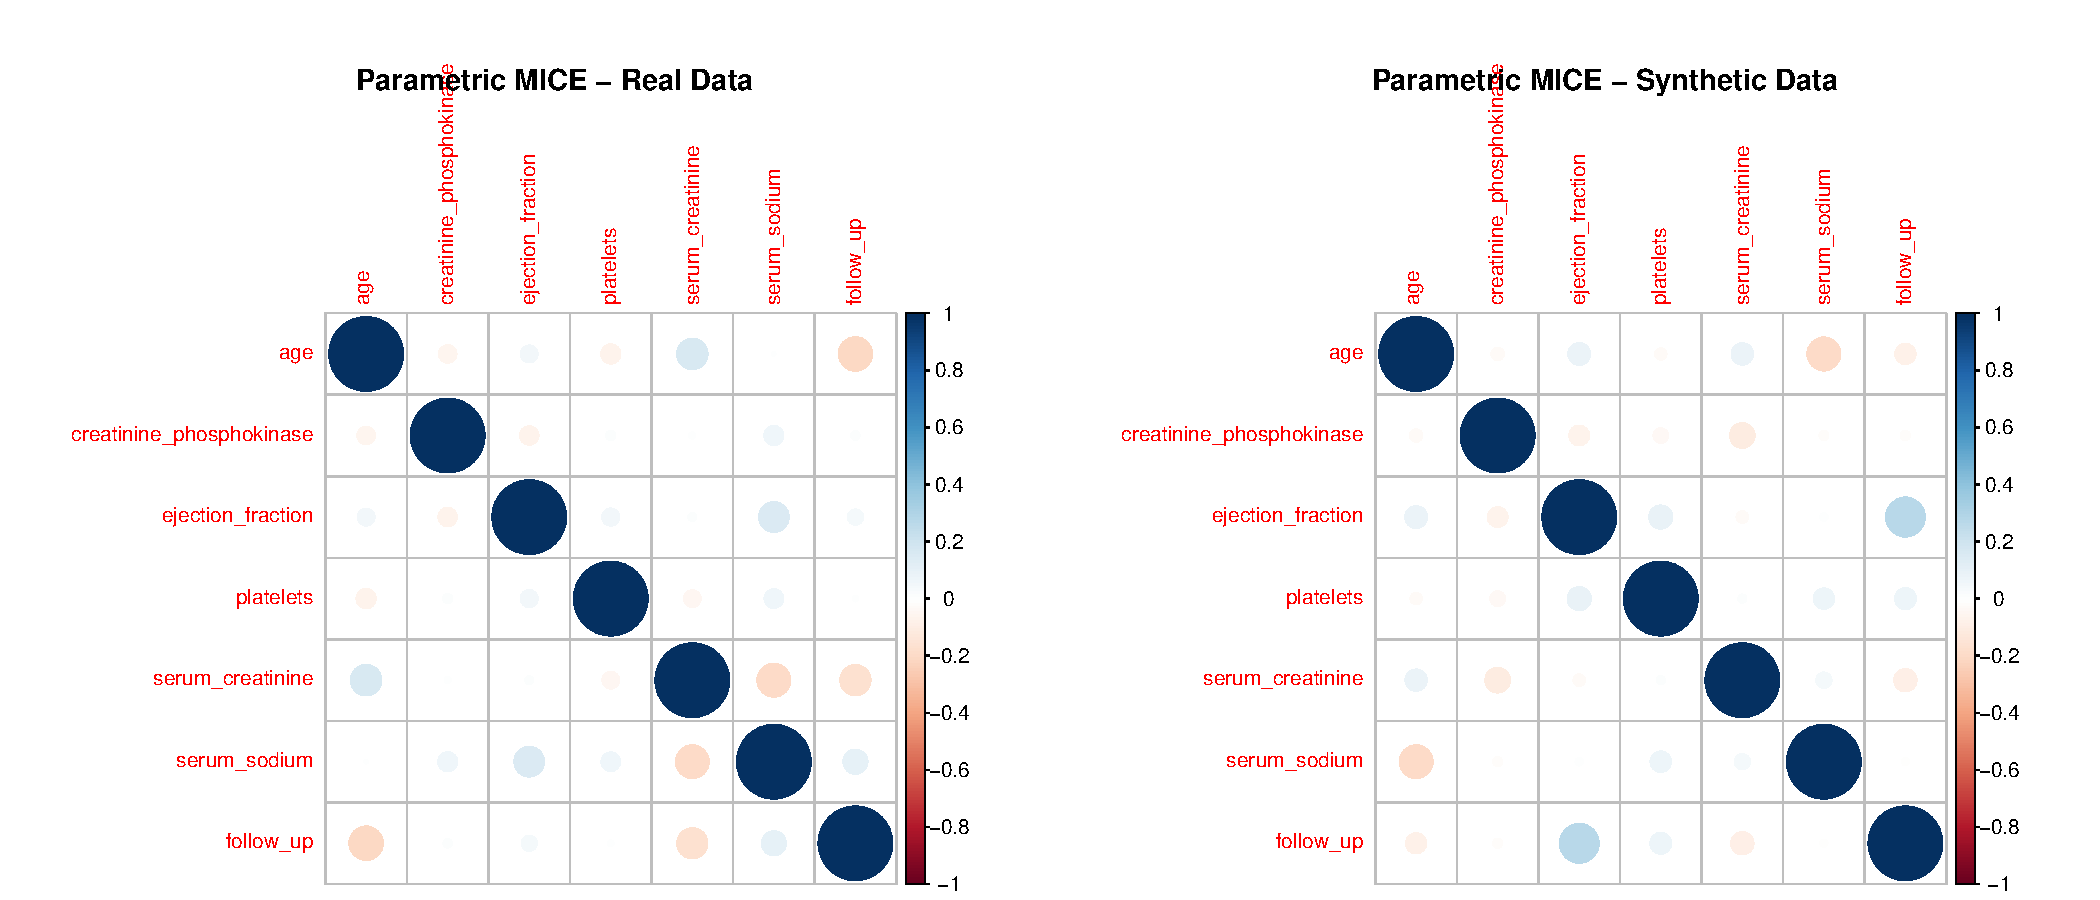
\includegraphics[width=1\linewidth,height=\textheight,keepaspectratio]{heart_failure_synthetic_data_project_files/figure-pdf/Correlation Matrices Comparison using Corrplot-1.pdf}
\end{center}

\begin{Shaded}
\begin{Highlighting}[]
\FunctionTok{compare\_correlation\_matrices}\NormalTok{(heart\_failure, syn\_cart\_1, }\StringTok{"CART Imputation"}\NormalTok{)}
\end{Highlighting}
\end{Shaded}

\begin{center}
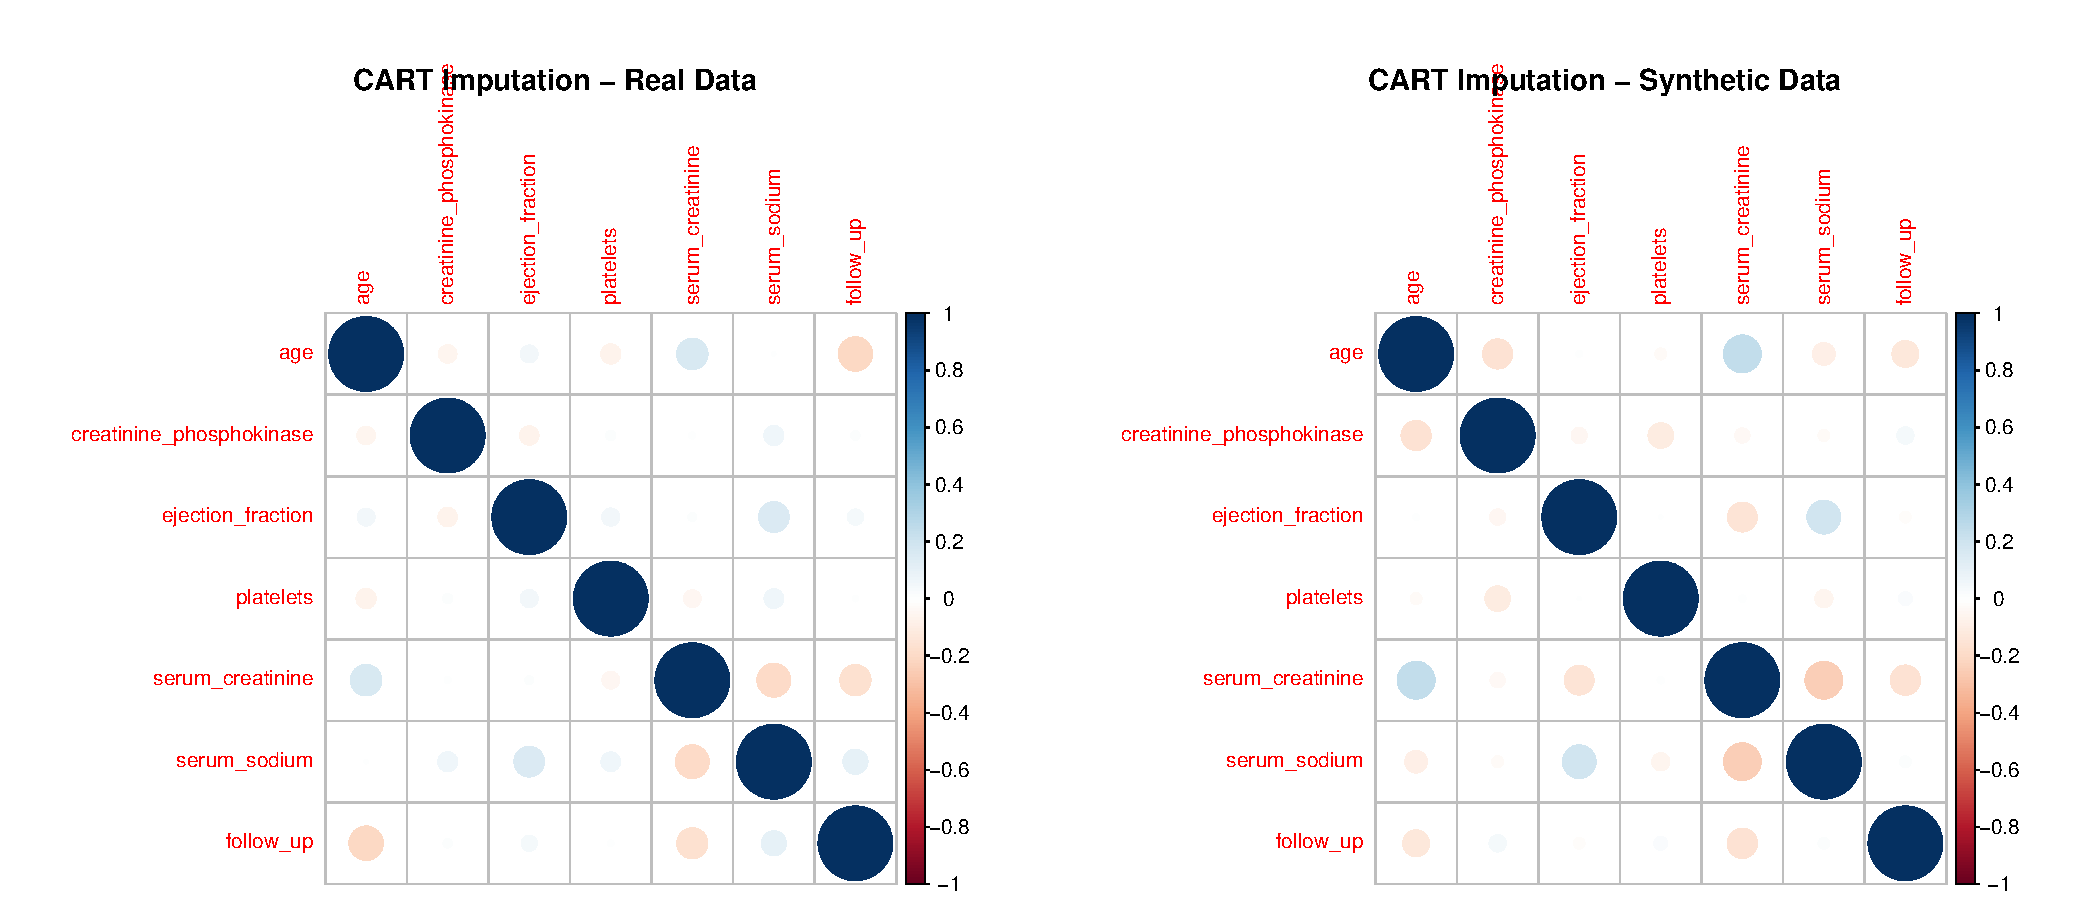
\includegraphics[width=1\linewidth,height=\textheight,keepaspectratio]{heart_failure_synthetic_data_project_files/figure-pdf/Correlation Matrices Comparison using Corrplot-2.pdf}
\end{center}

\begin{Shaded}
\begin{Highlighting}[]
\FunctionTok{compare\_correlation\_matrices}\NormalTok{(heart\_failure, syn\_data\_low\_fidelity\_synthpop, }\StringTok{"Synthpop (Low Fidelity)"}\NormalTok{)}
\end{Highlighting}
\end{Shaded}

\begin{center}
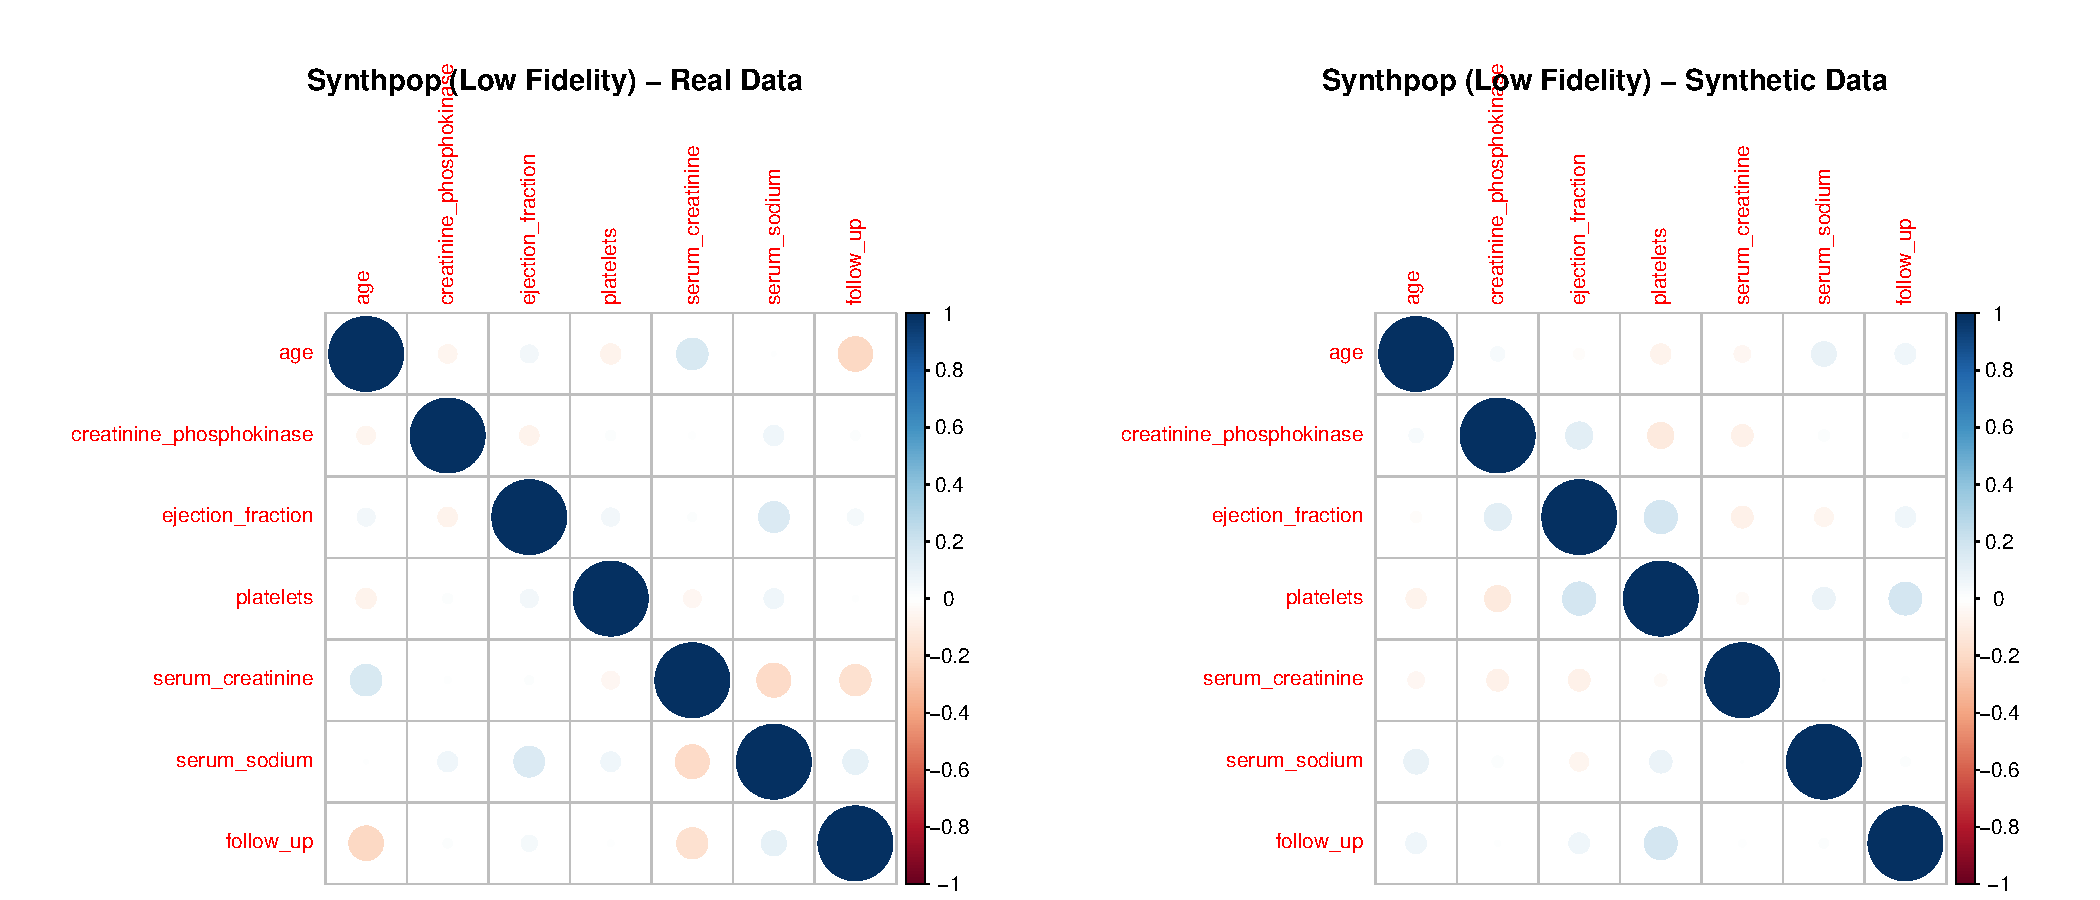
\includegraphics[width=1\linewidth,height=\textheight,keepaspectratio]{heart_failure_synthetic_data_project_files/figure-pdf/Correlation Matrices Comparison using Corrplot-3.pdf}
\end{center}

\begin{Shaded}
\begin{Highlighting}[]
\FunctionTok{compare\_correlation\_matrices}\NormalTok{(heart\_failure, syn\_data\_metadata, }\StringTok{"Metadata{-}Based"}\NormalTok{)}
\end{Highlighting}
\end{Shaded}

\begin{center}
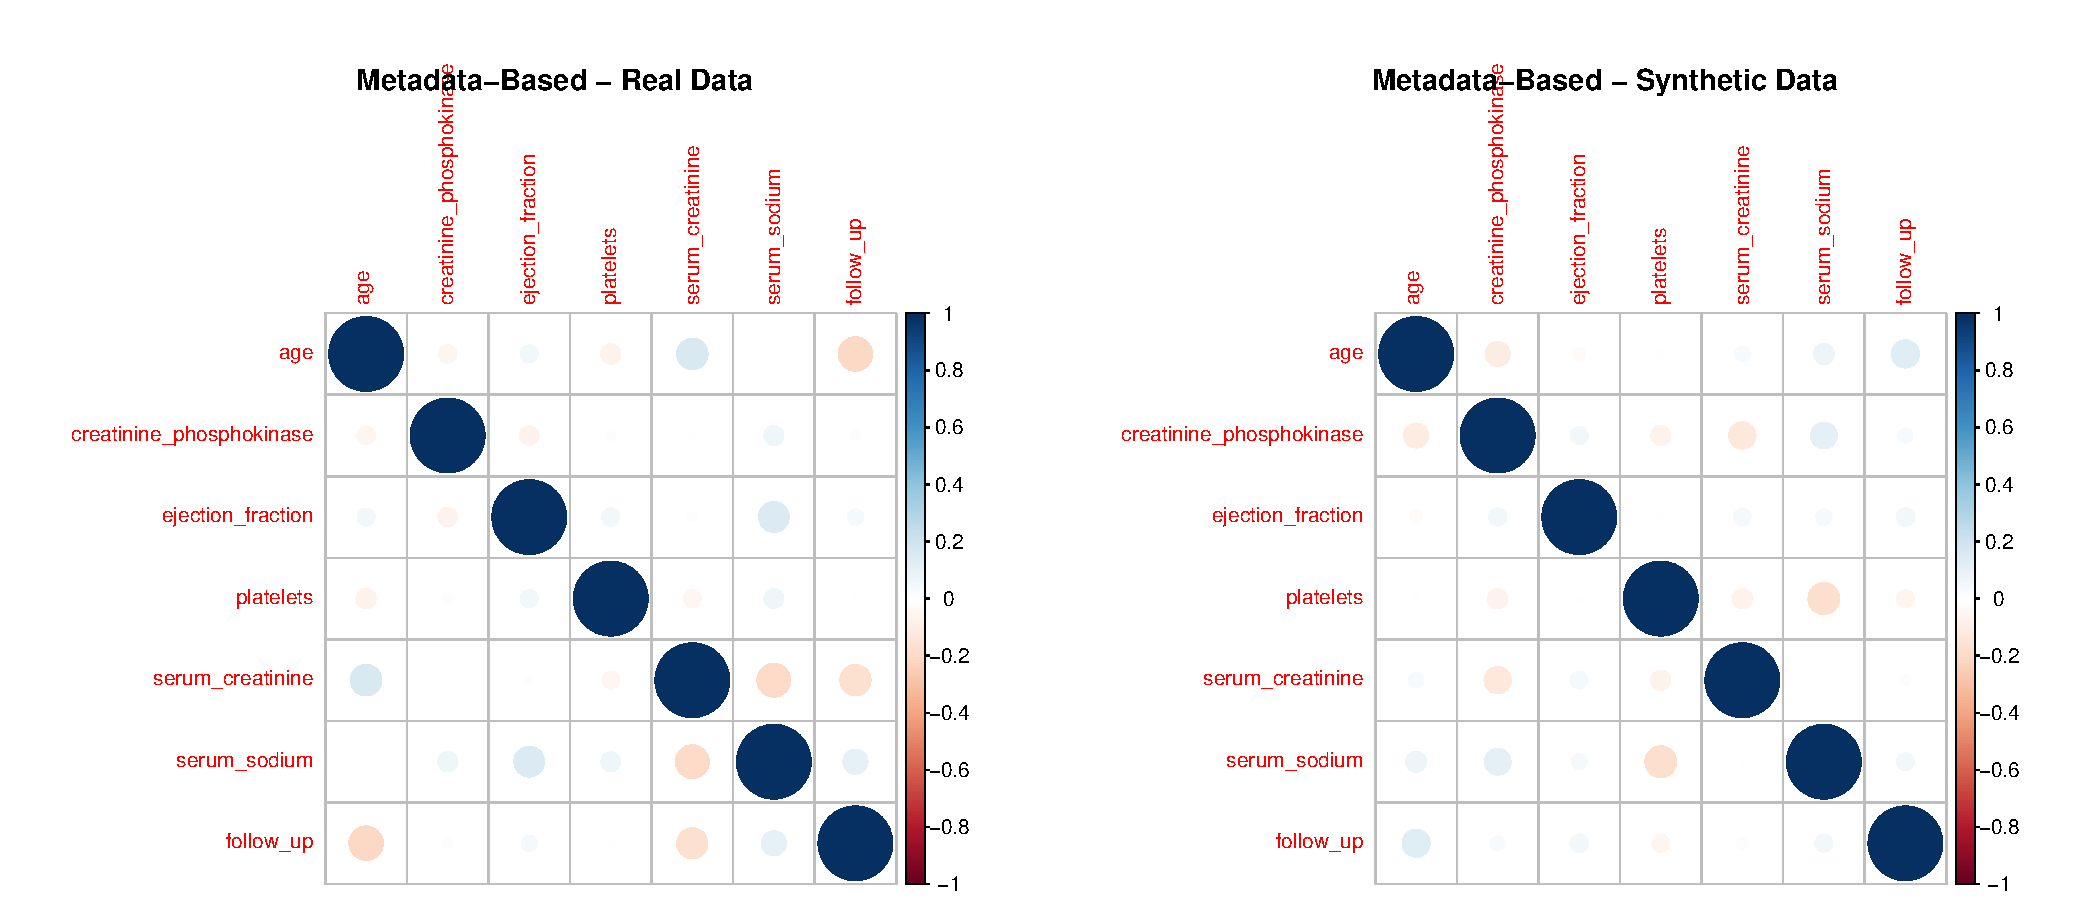
\includegraphics[width=1\linewidth,height=\textheight,keepaspectratio]{heart_failure_synthetic_data_project_files/figure-pdf/Correlation Matrices Comparison using Corrplot-4.pdf}
\end{center}

\paragraph{Correlation Matrices Comparison using
GGally}\label{correlation-matrices-comparison-using-ggally}

The \texttt{GGally} package extends \texttt{ggplot2} to create pairwise
visualizations, including correlation matrix plots. Using
\texttt{ggpairs()}, you can generate a matrix of scatterplots,
histograms, and correlation coefficients, which provides a detailed view
of the relationships between numeric variables in the real and synthetic
datasets.

\begin{Shaded}
\begin{Highlighting}[]
\NormalTok{compare\_correlation\_matrices\_ggally }\OtherTok{\textless{}{-}} \ControlFlowTok{function}\NormalTok{(real\_data, synthetic\_data, dataset\_name) \{}

  \CommentTok{\# Select only numeric columns from both datasets}
\NormalTok{  real\_numeric }\OtherTok{\textless{}{-}}\NormalTok{ real\_data }\SpecialCharTok{\%\textgreater{}\%} \FunctionTok{select}\NormalTok{(}\FunctionTok{where}\NormalTok{(is.numeric))}

  \CommentTok{\# Remove prefix \textquotesingle{}synth\_\textquotesingle{} from synthetic data column names}
  \FunctionTok{names}\NormalTok{(synthetic\_data) }\OtherTok{\textless{}{-}} \FunctionTok{gsub}\NormalTok{(}\StringTok{"\^{}synth\_"}\NormalTok{, }\StringTok{""}\NormalTok{, }\FunctionTok{names}\NormalTok{(synthetic\_data))}
\NormalTok{  synthetic\_numeric }\OtherTok{\textless{}{-}}\NormalTok{ synthetic\_data }\SpecialCharTok{\%\textgreater{}\%} \FunctionTok{select}\NormalTok{(}\FunctionTok{where}\NormalTok{(is.numeric))}

  \CommentTok{\# Ensure that both datasets have the same columns}
\NormalTok{  common\_columns }\OtherTok{\textless{}{-}} \FunctionTok{intersect}\NormalTok{(}\FunctionTok{names}\NormalTok{(real\_numeric), }\FunctionTok{names}\NormalTok{(synthetic\_numeric))}
  
  \ControlFlowTok{if}\NormalTok{ (}\FunctionTok{length}\NormalTok{(common\_columns) }\SpecialCharTok{==} \DecValTok{0}\NormalTok{) \{}
    \FunctionTok{cat}\NormalTok{(}\StringTok{"}\SpecialCharTok{\textbackslash{}n}\StringTok{No common numeric columns found for comparison in"}\NormalTok{, dataset\_name, }\StringTok{"}\SpecialCharTok{\textbackslash{}n}\StringTok{"}\NormalTok{)}
    \FunctionTok{return}\NormalTok{()}
\NormalTok{  \}}

\NormalTok{  real\_numeric }\OtherTok{\textless{}{-}}\NormalTok{ real\_numeric[, common\_columns, drop }\OtherTok{=} \ConstantTok{FALSE}\NormalTok{]}
\NormalTok{  synthetic\_numeric }\OtherTok{\textless{}{-}}\NormalTok{ synthetic\_numeric[, common\_columns, drop }\OtherTok{=} \ConstantTok{FALSE}\NormalTok{]}

  \CommentTok{\# Add a column to differentiate between real and synthetic data}
\NormalTok{  real\_numeric}\SpecialCharTok{$}\NormalTok{Dataset }\OtherTok{\textless{}{-}} \StringTok{"Real"}
\NormalTok{  synthetic\_numeric}\SpecialCharTok{$}\NormalTok{Dataset }\OtherTok{\textless{}{-}} \StringTok{"Synth"}

  \CommentTok{\# Combine the datasets}
\NormalTok{  combined\_data }\OtherTok{\textless{}{-}} \FunctionTok{rbind}\NormalTok{(real\_numeric, synthetic\_numeric)}

  \CommentTok{\# Create correlation matrix plot using GGally if there are valid columns to plot}
  \ControlFlowTok{if}\NormalTok{ (}\FunctionTok{ncol}\NormalTok{(combined\_data) }\SpecialCharTok{\textgreater{}} \DecValTok{1}\NormalTok{) \{}
\NormalTok{    p }\OtherTok{\textless{}{-}} \FunctionTok{ggpairs}\NormalTok{(}
\NormalTok{      combined\_data, }
      \FunctionTok{aes}\NormalTok{(}\AttributeTok{color =}\NormalTok{ Dataset, }\AttributeTok{alpha =} \FloatTok{0.5}\NormalTok{), }
      \AttributeTok{title =} \FunctionTok{paste}\NormalTok{(dataset\_name, }\StringTok{"{-} Correlation Matrix Comparison"}\NormalTok{),}
      \AttributeTok{columns =} \DecValTok{1}\SpecialCharTok{:}\NormalTok{(}\FunctionTok{ncol}\NormalTok{(combined\_data) }\SpecialCharTok{{-}} \DecValTok{1}\NormalTok{),  }\CommentTok{\# Exclude the \textquotesingle{}Dataset\textquotesingle{} column from the plot}
      \AttributeTok{upper =} \FunctionTok{list}\NormalTok{(}\AttributeTok{continuous =} \FunctionTok{wrap}\NormalTok{(}\StringTok{"cor"}\NormalTok{, }\AttributeTok{size =} \DecValTok{3}\NormalTok{, }\AttributeTok{alignPercent =} \FloatTok{0.5}\NormalTok{)),  }\CommentTok{\# Smaller correlation labels}
      \AttributeTok{lower =} \FunctionTok{list}\NormalTok{(}\AttributeTok{continuous =} \FunctionTok{wrap}\NormalTok{(}\StringTok{"smooth"}\NormalTok{, }\AttributeTok{alpha =} \FloatTok{0.4}\NormalTok{, }\AttributeTok{size =} \FloatTok{0.5}\NormalTok{)),  }\CommentTok{\# Smoother plots for readability}
      \AttributeTok{diag =} \FunctionTok{list}\NormalTok{(}\AttributeTok{continuous =} \FunctionTok{wrap}\NormalTok{(}\StringTok{"densityDiag"}\NormalTok{, }\AttributeTok{alpha =} \FloatTok{0.5}\NormalTok{))  }\CommentTok{\# Density plot with improved transparency}
\NormalTok{    ) }\SpecialCharTok{+}
      \FunctionTok{theme\_minimal}\NormalTok{() }\SpecialCharTok{+}  \CommentTok{\# Use a cleaner theme}
      \FunctionTok{theme}\NormalTok{(}
        \AttributeTok{strip.text =} \FunctionTok{element\_text}\NormalTok{(}\AttributeTok{size =} \DecValTok{8}\NormalTok{, }\AttributeTok{face =} \StringTok{"bold"}\NormalTok{),  }\CommentTok{\# Smaller strip labels}
        \AttributeTok{axis.text.x =} \FunctionTok{element\_text}\NormalTok{(}\AttributeTok{angle =} \DecValTok{45}\NormalTok{, }\AttributeTok{hjust =} \DecValTok{1}\NormalTok{, }\AttributeTok{size =} \DecValTok{7}\NormalTok{),  }\CommentTok{\# Rotate x{-}axis labels for better readability}
        \AttributeTok{axis.text.y =} \FunctionTok{element\_text}\NormalTok{(}\AttributeTok{size =} \DecValTok{7}\NormalTok{),}
        \AttributeTok{legend.position =} \StringTok{"top"}\NormalTok{,  }\CommentTok{\# Move legend to a better location}
        \AttributeTok{legend.title =} \FunctionTok{element\_blank}\NormalTok{()  }\CommentTok{\# Remove unnecessary legend title}
\NormalTok{      )}
    \FunctionTok{print}\NormalTok{(p)}
\NormalTok{  \} }\ControlFlowTok{else}\NormalTok{ \{}
    \FunctionTok{cat}\NormalTok{(}\StringTok{"}\SpecialCharTok{\textbackslash{}n}\StringTok{Not enough numeric columns to generate a correlation matrix plot for"}\NormalTok{, dataset\_name, }\StringTok{"}\SpecialCharTok{\textbackslash{}n}\StringTok{"}\NormalTok{)}
\NormalTok{  \}}
\NormalTok{\}}

\CommentTok{\# Apply the function to each synthetic dataset}
\FunctionTok{compare\_correlation\_matrices\_ggally}\NormalTok{(heart\_failure, syn\_data\_1, }\StringTok{"Parametric MICE"}\NormalTok{)}
\end{Highlighting}
\end{Shaded}

\begin{center}
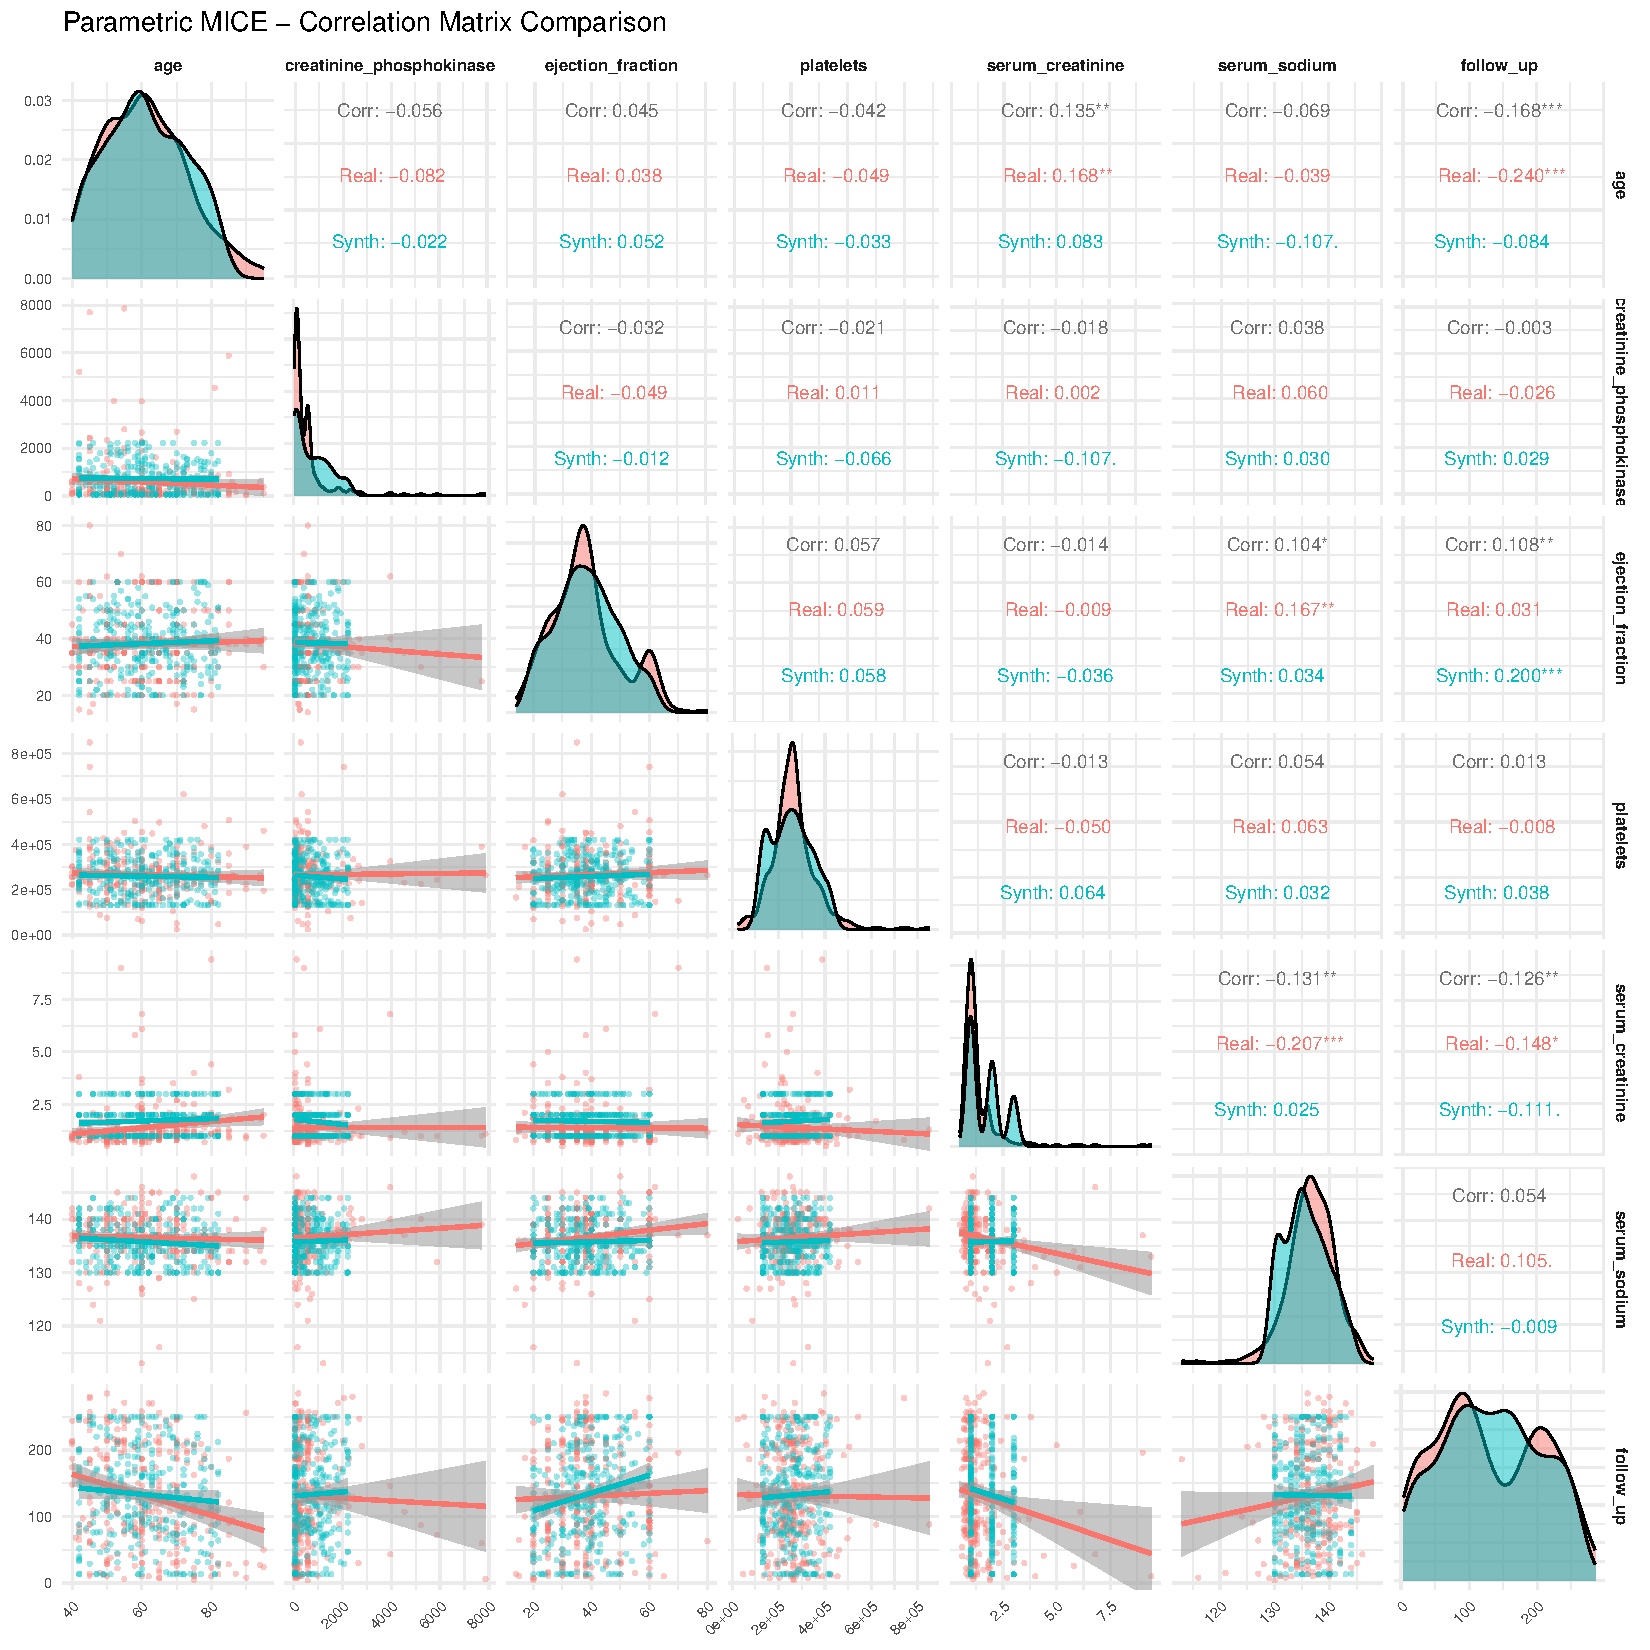
\includegraphics[width=1\linewidth,height=\textheight,keepaspectratio]{heart_failure_synthetic_data_project_files/figure-pdf/Correlation Matrices Comparison using GGally-1.pdf}
\end{center}

\begin{Shaded}
\begin{Highlighting}[]
\FunctionTok{compare\_correlation\_matrices\_ggally}\NormalTok{(heart\_failure, syn\_cart\_1, }\StringTok{"CART Imputation"}\NormalTok{)}
\end{Highlighting}
\end{Shaded}

\begin{center}
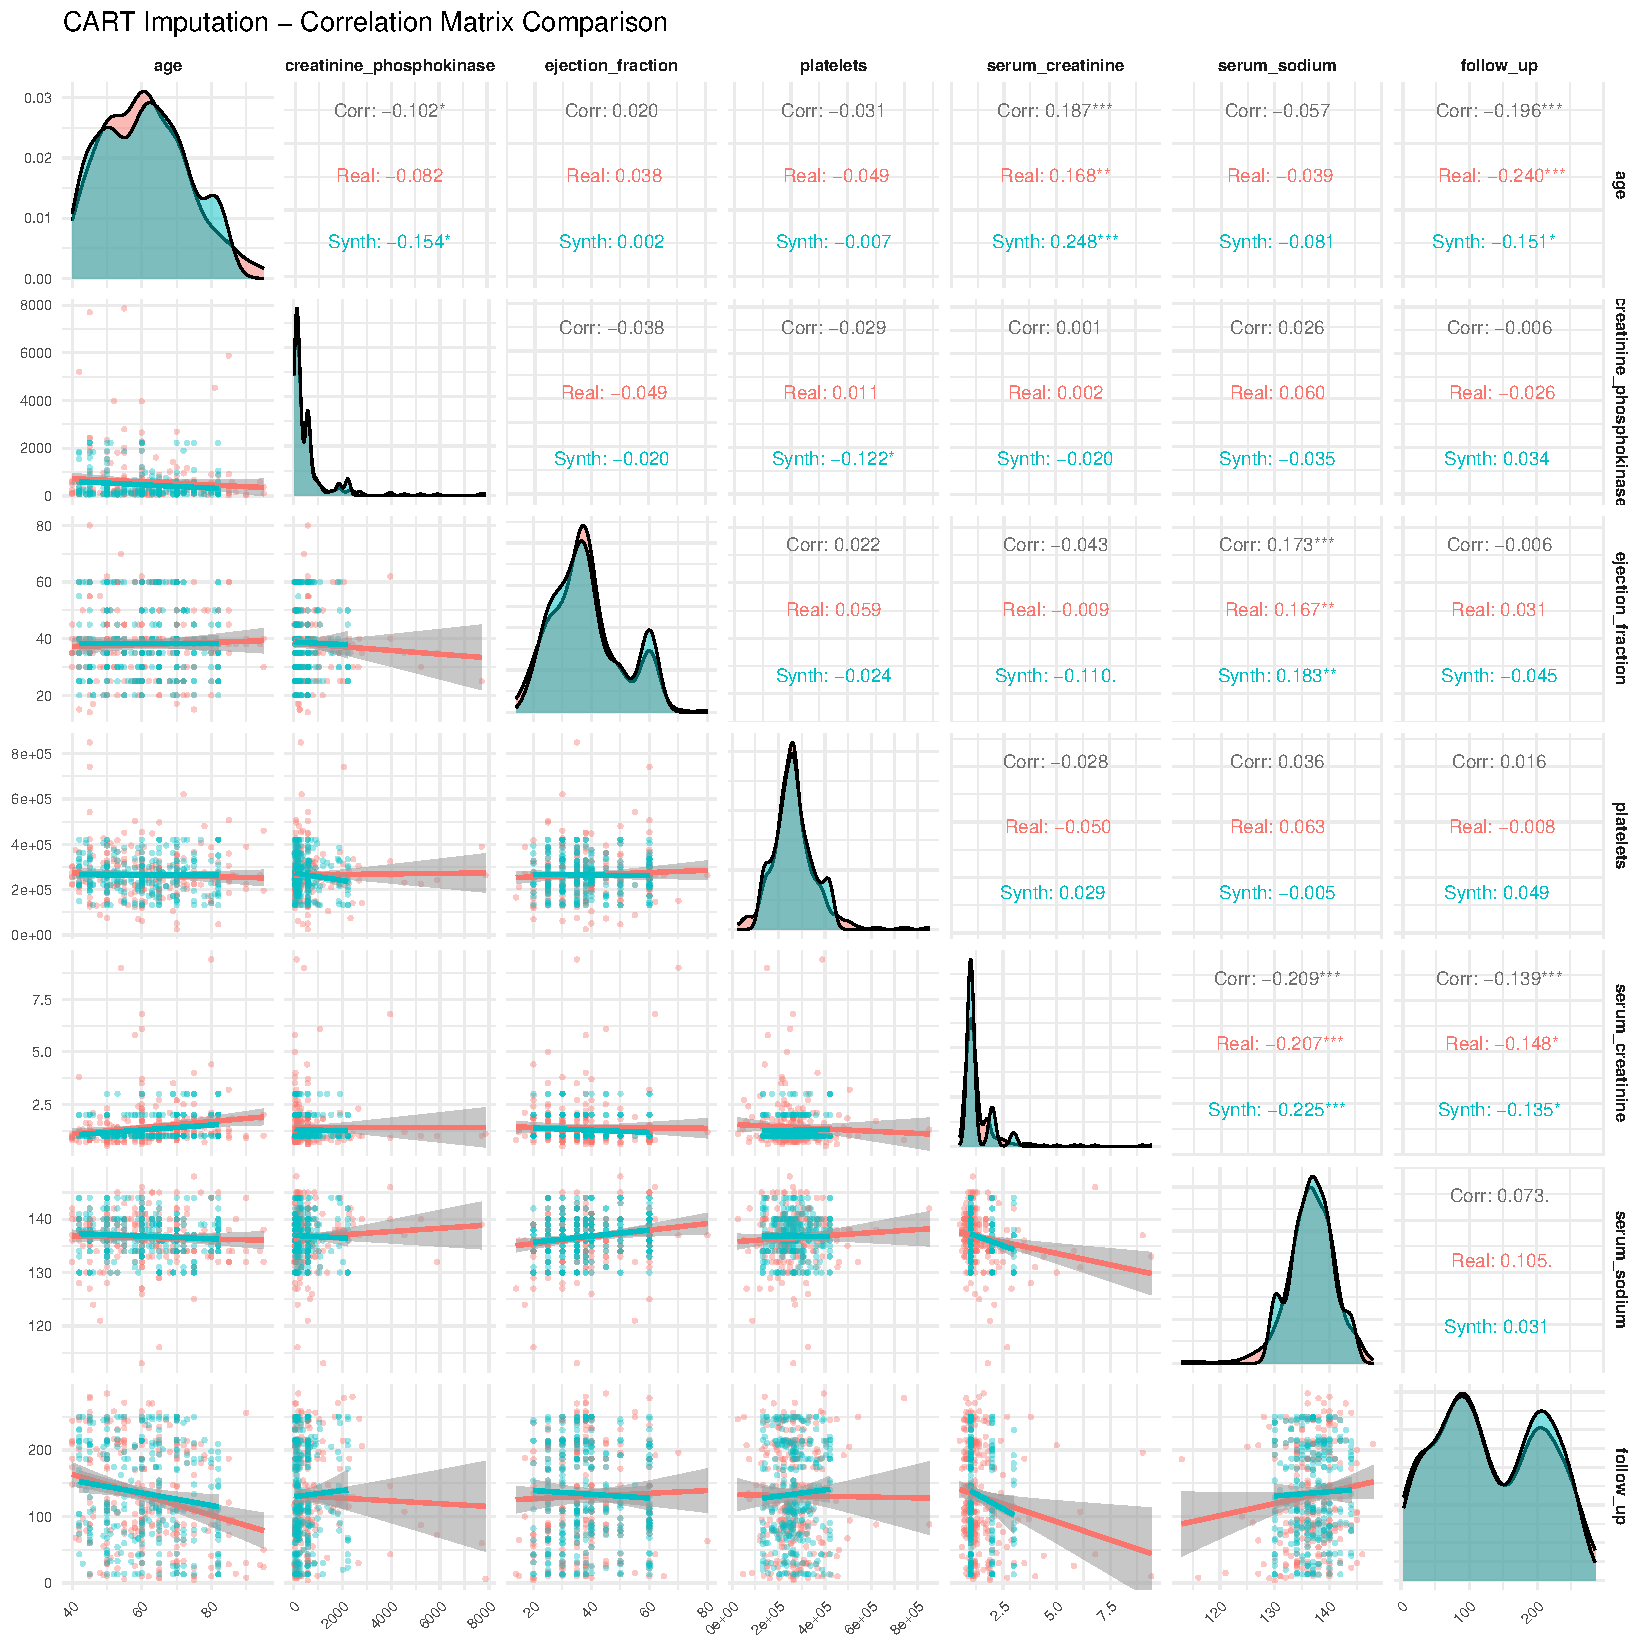
\includegraphics[width=1\linewidth,height=\textheight,keepaspectratio]{heart_failure_synthetic_data_project_files/figure-pdf/Correlation Matrices Comparison using GGally-2.pdf}
\end{center}

\begin{Shaded}
\begin{Highlighting}[]
\FunctionTok{compare\_correlation\_matrices\_ggally}\NormalTok{(heart\_failure, syn\_data\_low\_fidelity\_synthpop, }\StringTok{"Synthpop Low Fidelity"}\NormalTok{)}
\end{Highlighting}
\end{Shaded}

\begin{center}
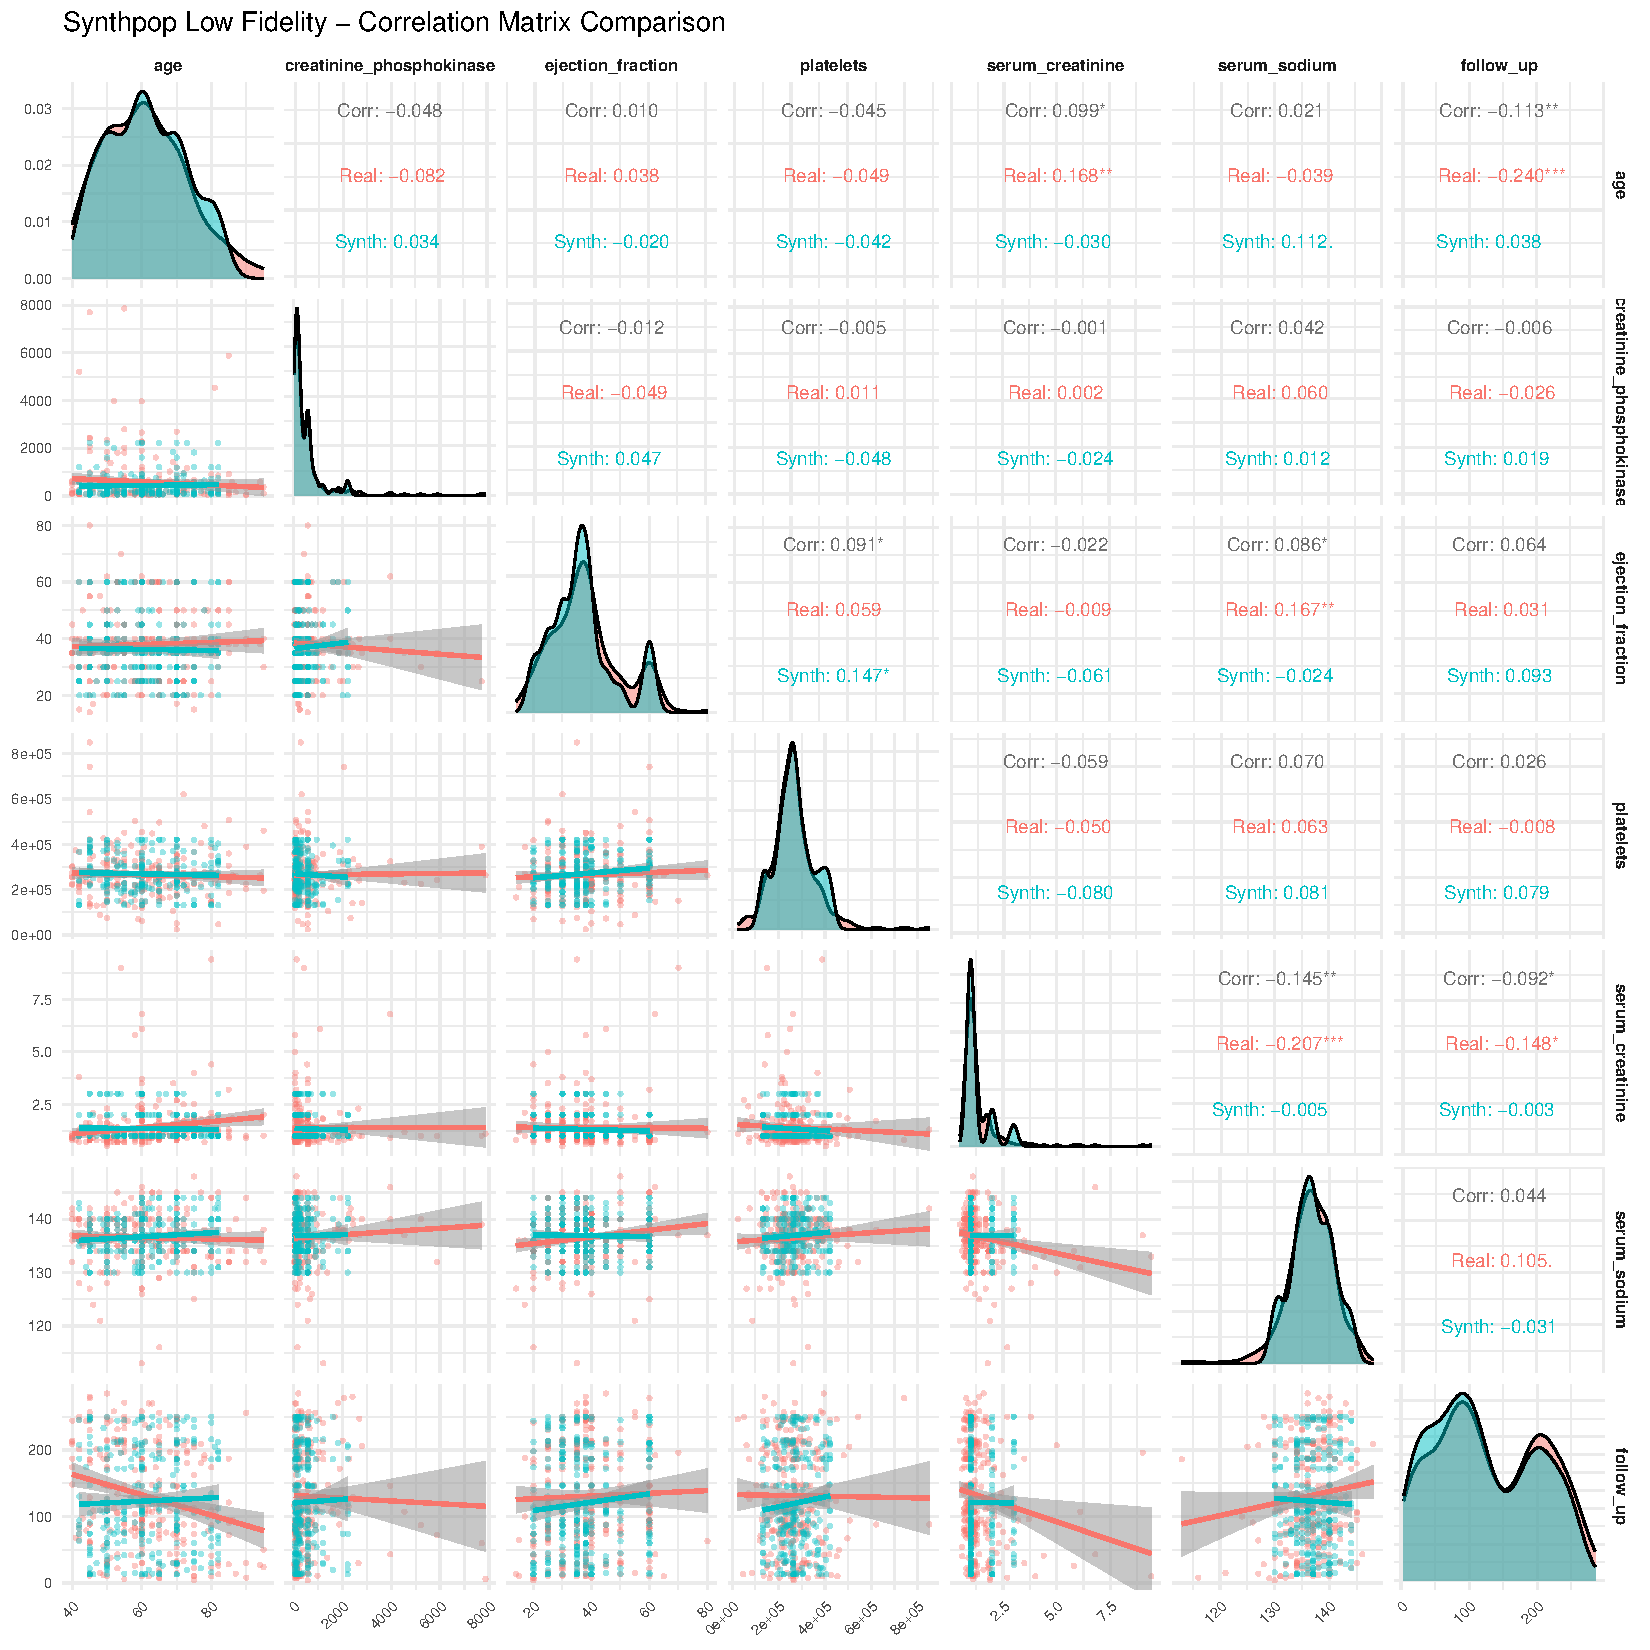
\includegraphics[width=1\linewidth,height=\textheight,keepaspectratio]{heart_failure_synthetic_data_project_files/figure-pdf/Correlation Matrices Comparison using GGally-3.pdf}
\end{center}

\begin{Shaded}
\begin{Highlighting}[]
\FunctionTok{compare\_correlation\_matrices\_ggally}\NormalTok{(heart\_failure, syn\_data\_metadata, }\StringTok{"Metadata{-}Based Synthetic Data"}\NormalTok{)}
\end{Highlighting}
\end{Shaded}

\begin{center}
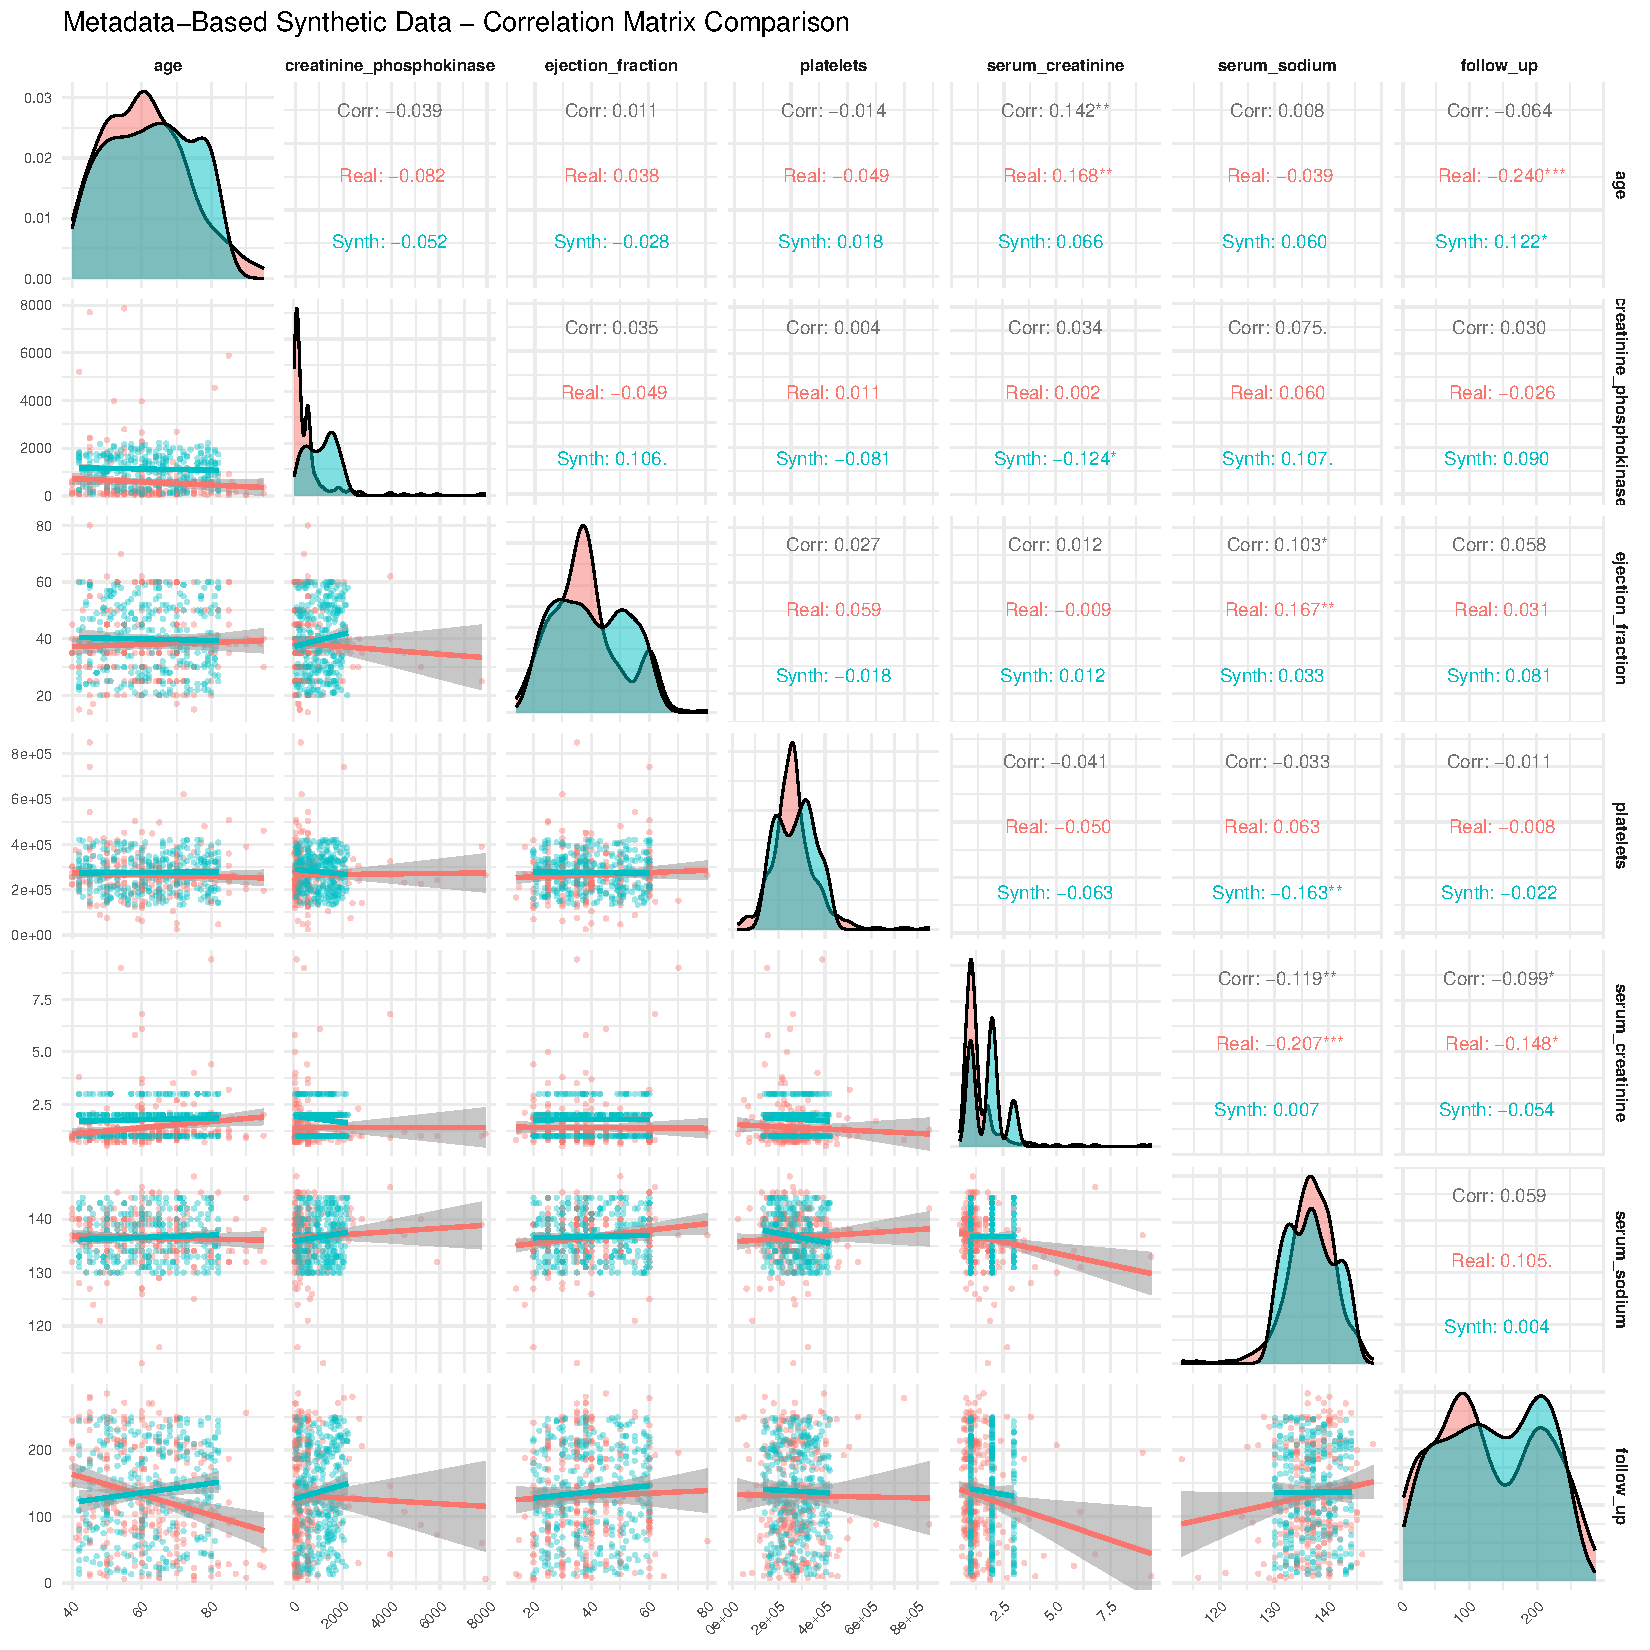
\includegraphics[width=1\linewidth,height=\textheight,keepaspectratio]{heart_failure_synthetic_data_project_files/figure-pdf/Correlation Matrices Comparison using GGally-4.pdf}
\end{center}

\subsection{Fidelity Assessment}\label{fidelity-assessment}

\subsubsection{Descriptive Statistics}\label{descriptive-statistics}

This section provides a comparative analysis of the descriptive
statistics between the real dataset and the synthetic datasets generated
using different methods.

\paragraph{Real Dataset}\label{real-dataset}

The descriptive statistics for the real heart failure dataset include
metrics such as mean, median, standard deviation, and range. This serves
as the baseline for comparison with the synthetic datasets.

\begin{Shaded}
\begin{Highlighting}[]
\CommentTok{\# Generate descriptive stats}
\NormalTok{desc\_tbl }\OtherTok{\textless{}{-}} \FunctionTok{describe}\NormalTok{(heart\_failure) }\SpecialCharTok{\%\textgreater{}\%}
  \FunctionTok{as.data.frame}\NormalTok{() }\SpecialCharTok{\%\textgreater{}\%}
  \FunctionTok{select}\NormalTok{(n, mean, sd, min, median, max) }\SpecialCharTok{\%\textgreater{}\%}
  \FunctionTok{round}\NormalTok{(}\DecValTok{2}\NormalTok{) }\SpecialCharTok{\%\textgreater{}\%}
\NormalTok{  tibble}\SpecialCharTok{::}\FunctionTok{rownames\_to\_column}\NormalTok{(}\StringTok{"Variable"}\NormalTok{)}

\CommentTok{\# Display as a neat table}
\FunctionTok{kable}\NormalTok{(}
\NormalTok{  desc\_tbl,}
  \AttributeTok{caption =} \StringTok{"Descriptive Statistics for the Heart Failure Dataset"}\NormalTok{,}
  \AttributeTok{align =} \StringTok{"lrrrrrr"}
\NormalTok{)}
\end{Highlighting}
\end{Shaded}

\begin{longtable}[]{@{}
  >{\raggedright\arraybackslash}p{(\linewidth - 12\tabcolsep) * \real{0.3378}}
  >{\raggedleft\arraybackslash}p{(\linewidth - 12\tabcolsep) * \real{0.0541}}
  >{\raggedleft\arraybackslash}p{(\linewidth - 12\tabcolsep) * \real{0.1351}}
  >{\raggedleft\arraybackslash}p{(\linewidth - 12\tabcolsep) * \real{0.1216}}
  >{\raggedleft\arraybackslash}p{(\linewidth - 12\tabcolsep) * \real{0.1081}}
  >{\raggedleft\arraybackslash}p{(\linewidth - 12\tabcolsep) * \real{0.1216}}
  >{\raggedleft\arraybackslash}p{(\linewidth - 12\tabcolsep) * \real{0.1216}}@{}}
\caption{Descriptive Statistics for the Heart Failure
Dataset}\tabularnewline
\toprule\noalign{}
\begin{minipage}[b]{\linewidth}\raggedright
Variable
\end{minipage} & \begin{minipage}[b]{\linewidth}\raggedleft
n
\end{minipage} & \begin{minipage}[b]{\linewidth}\raggedleft
mean
\end{minipage} & \begin{minipage}[b]{\linewidth}\raggedleft
sd
\end{minipage} & \begin{minipage}[b]{\linewidth}\raggedleft
min
\end{minipage} & \begin{minipage}[b]{\linewidth}\raggedleft
median
\end{minipage} & \begin{minipage}[b]{\linewidth}\raggedleft
max
\end{minipage} \\
\midrule\noalign{}
\endfirsthead
\toprule\noalign{}
\begin{minipage}[b]{\linewidth}\raggedright
Variable
\end{minipage} & \begin{minipage}[b]{\linewidth}\raggedleft
n
\end{minipage} & \begin{minipage}[b]{\linewidth}\raggedleft
mean
\end{minipage} & \begin{minipage}[b]{\linewidth}\raggedleft
sd
\end{minipage} & \begin{minipage}[b]{\linewidth}\raggedleft
min
\end{minipage} & \begin{minipage}[b]{\linewidth}\raggedleft
median
\end{minipage} & \begin{minipage}[b]{\linewidth}\raggedleft
max
\end{minipage} \\
\midrule\noalign{}
\endhead
\bottomrule\noalign{}
\endlastfoot
age & 284 & 60.80 & 12.08 & 40.0 & 60.0 & 95.0 \\
anaemia* & 299 & 1.43 & 0.50 & 1.0 & 1.0 & 2.0 \\
creatinine\_phosphokinase & 285 & 578.81 & 981.99 & 23.0 & 249.0 &
7861.0 \\
diabetes* & 299 & 1.42 & 0.49 & 1.0 & 1.0 & 2.0 \\
ejection\_fraction & 287 & 38.00 & 11.92 & 14.0 & 38.0 & 80.0 \\
platelets & 285 & 265163.83 & 97508.63 & 25100.0 & 263358.0 &
850000.0 \\
serum\_creatinine & 281 & 1.39 & 1.05 & 0.5 & 1.1 & 9.4 \\
serum\_sodium & 279 & 136.59 & 4.49 & 113.0 & 137.0 & 148.0 \\
sex* & 299 & 1.65 & 0.48 & 1.0 & 2.0 & 2.0 \\
smoking* & 299 & 1.32 & 0.47 & 1.0 & 1.0 & 2.0 \\
hypertension* & 299 & 1.35 & 0.48 & 1.0 & 1.0 & 2.0 \\
deceased* & 299 & 1.32 & 0.47 & 1.0 & 1.0 & 2.0 \\
follow\_up & 299 & 130.26 & 77.61 & 4.0 & 115.0 & 285.0 \\
\end{longtable}

\paragraph{Parametric Imputation
(MICE)}\label{parametric-imputation-mice}

The synthetic data generated using the MICE framework is analyzed to
compare its summary statistics with the real dataset. This will help
evaluate how well the parametric method captures the key characteristics
of the data.

\begin{Shaded}
\begin{Highlighting}[]
\CommentTok{\# Descriptive stats for Parametric MICE synthetic dataset}
\NormalTok{desc\_mice }\OtherTok{\textless{}{-}} \FunctionTok{describe}\NormalTok{(syn\_data\_1) }\SpecialCharTok{\%\textgreater{}\%}
  \FunctionTok{as.data.frame}\NormalTok{() }\SpecialCharTok{\%\textgreater{}\%}
  \FunctionTok{select}\NormalTok{(n, mean, sd, min, median, max) }\SpecialCharTok{\%\textgreater{}\%}
  \FunctionTok{round}\NormalTok{(}\DecValTok{2}\NormalTok{) }\SpecialCharTok{\%\textgreater{}\%}
\NormalTok{  tibble}\SpecialCharTok{::}\FunctionTok{rownames\_to\_column}\NormalTok{(}\StringTok{"Variable"}\NormalTok{)}

\CommentTok{\# Display table}
\FunctionTok{kable}\NormalTok{(}
\NormalTok{  desc\_mice,}
  \AttributeTok{caption =} \StringTok{"Descriptive Statistics for Parametric MICE Synthetic Dataset"}\NormalTok{,}
  \AttributeTok{align =} \StringTok{"lrrrrrr"}
\NormalTok{)}
\end{Highlighting}
\end{Shaded}

\begin{longtable}[]{@{}
  >{\raggedright\arraybackslash}p{(\linewidth - 12\tabcolsep) * \real{0.4133}}
  >{\raggedleft\arraybackslash}p{(\linewidth - 12\tabcolsep) * \real{0.0533}}
  >{\raggedleft\arraybackslash}p{(\linewidth - 12\tabcolsep) * \real{0.1333}}
  >{\raggedleft\arraybackslash}p{(\linewidth - 12\tabcolsep) * \real{0.1200}}
  >{\raggedleft\arraybackslash}p{(\linewidth - 12\tabcolsep) * \real{0.0933}}
  >{\raggedleft\arraybackslash}p{(\linewidth - 12\tabcolsep) * \real{0.0933}}
  >{\raggedleft\arraybackslash}p{(\linewidth - 12\tabcolsep) * \real{0.0933}}@{}}
\caption{Descriptive Statistics for Parametric MICE Synthetic
Dataset}\tabularnewline
\toprule\noalign{}
\begin{minipage}[b]{\linewidth}\raggedright
Variable
\end{minipage} & \begin{minipage}[b]{\linewidth}\raggedleft
n
\end{minipage} & \begin{minipage}[b]{\linewidth}\raggedleft
mean
\end{minipage} & \begin{minipage}[b]{\linewidth}\raggedleft
sd
\end{minipage} & \begin{minipage}[b]{\linewidth}\raggedleft
min
\end{minipage} & \begin{minipage}[b]{\linewidth}\raggedleft
median
\end{minipage} & \begin{minipage}[b]{\linewidth}\raggedleft
max
\end{minipage} \\
\midrule\noalign{}
\endfirsthead
\toprule\noalign{}
\begin{minipage}[b]{\linewidth}\raggedright
Variable
\end{minipage} & \begin{minipage}[b]{\linewidth}\raggedleft
n
\end{minipage} & \begin{minipage}[b]{\linewidth}\raggedleft
mean
\end{minipage} & \begin{minipage}[b]{\linewidth}\raggedleft
sd
\end{minipage} & \begin{minipage}[b]{\linewidth}\raggedleft
min
\end{minipage} & \begin{minipage}[b]{\linewidth}\raggedleft
median
\end{minipage} & \begin{minipage}[b]{\linewidth}\raggedleft
max
\end{minipage} \\
\midrule\noalign{}
\endhead
\bottomrule\noalign{}
\endlastfoot
synth\_age & 284 & 61.01 & 11.40 & 42 & 60 & 82 \\
synth\_anaemia* & 299 & 1.45 & 0.50 & 1 & 1 & 2 \\
synth\_creatinine\_phosphokinase & 285 & 735.72 & 687.98 & 59 & 540 &
2221 \\
synth\_diabetes* & 299 & 1.42 & 0.49 & 1 & 1 & 2 \\
synth\_ejection\_fraction & 287 & 38.44 & 10.70 & 20 & 38 & 60 \\
synth\_platelets & 285 & 257523.78 & 86505.14 & 132200 & 254087 &
421200 \\
synth\_serum\_creatinine & 281 & 1.70 & 0.77 & 1 & 2 & 3 \\
synth\_serum\_sodium & 279 & 135.78 & 3.96 & 130 & 135 & 144 \\
synth\_sex* & 299 & 1.64 & 0.48 & 1 & 2 & 2 \\
synth\_smoking* & 299 & 1.29 & 0.45 & 1 & 1 & 2 \\
synth\_hypertension* & 299 & 1.42 & 0.49 & 1 & 1 & 2 \\
synth\_deceased* & 299 & 1.31 & 0.47 & 1 & 1 & 2 \\
synth\_follow\_up & 299 & 132.74 & 71.11 & 13 & 132 & 250 \\
\end{longtable}

\paragraph{Non-Parametric Imputation
(CART)}\label{non-parametric-imputation-cart}

The CART method is a non-parametric technique that handles non-linear
relationships. The descriptive statistics of the CART-imputed synthetic
data provide insight into how this method captures the dataset's
distribution.

\begin{Shaded}
\begin{Highlighting}[]
\CommentTok{\# Descriptive stats for CART synthetic dataset}
\NormalTok{desc\_cart }\OtherTok{\textless{}{-}} \FunctionTok{describe}\NormalTok{(syn\_cart\_1) }\SpecialCharTok{\%\textgreater{}\%}
  \FunctionTok{as.data.frame}\NormalTok{() }\SpecialCharTok{\%\textgreater{}\%}
  \FunctionTok{select}\NormalTok{(n, mean, sd, min, median, max) }\SpecialCharTok{\%\textgreater{}\%}
  \FunctionTok{round}\NormalTok{(}\DecValTok{2}\NormalTok{) }\SpecialCharTok{\%\textgreater{}\%}
\NormalTok{  tibble}\SpecialCharTok{::}\FunctionTok{rownames\_to\_column}\NormalTok{(}\StringTok{"Variable"}\NormalTok{)}

\CommentTok{\# Display table}
\FunctionTok{kable}\NormalTok{(}
\NormalTok{  desc\_cart,}
  \AttributeTok{caption =} \StringTok{"Descriptive Statistics for CART Synthetic Dataset"}\NormalTok{,}
  \AttributeTok{align =} \StringTok{"lrrrrrr"}
\NormalTok{)}
\end{Highlighting}
\end{Shaded}

\begin{longtable}[]{@{}
  >{\raggedright\arraybackslash}p{(\linewidth - 12\tabcolsep) * \real{0.4133}}
  >{\raggedleft\arraybackslash}p{(\linewidth - 12\tabcolsep) * \real{0.0533}}
  >{\raggedleft\arraybackslash}p{(\linewidth - 12\tabcolsep) * \real{0.1333}}
  >{\raggedleft\arraybackslash}p{(\linewidth - 12\tabcolsep) * \real{0.1200}}
  >{\raggedleft\arraybackslash}p{(\linewidth - 12\tabcolsep) * \real{0.0933}}
  >{\raggedleft\arraybackslash}p{(\linewidth - 12\tabcolsep) * \real{0.0933}}
  >{\raggedleft\arraybackslash}p{(\linewidth - 12\tabcolsep) * \real{0.0933}}@{}}
\caption{Descriptive Statistics for CART Synthetic
Dataset}\tabularnewline
\toprule\noalign{}
\begin{minipage}[b]{\linewidth}\raggedright
Variable
\end{minipage} & \begin{minipage}[b]{\linewidth}\raggedleft
n
\end{minipage} & \begin{minipage}[b]{\linewidth}\raggedleft
mean
\end{minipage} & \begin{minipage}[b]{\linewidth}\raggedleft
sd
\end{minipage} & \begin{minipage}[b]{\linewidth}\raggedleft
min
\end{minipage} & \begin{minipage}[b]{\linewidth}\raggedleft
median
\end{minipage} & \begin{minipage}[b]{\linewidth}\raggedleft
max
\end{minipage} \\
\midrule\noalign{}
\endfirsthead
\toprule\noalign{}
\begin{minipage}[b]{\linewidth}\raggedright
Variable
\end{minipage} & \begin{minipage}[b]{\linewidth}\raggedleft
n
\end{minipage} & \begin{minipage}[b]{\linewidth}\raggedleft
mean
\end{minipage} & \begin{minipage}[b]{\linewidth}\raggedleft
sd
\end{minipage} & \begin{minipage}[b]{\linewidth}\raggedleft
min
\end{minipage} & \begin{minipage}[b]{\linewidth}\raggedleft
median
\end{minipage} & \begin{minipage}[b]{\linewidth}\raggedleft
max
\end{minipage} \\
\midrule\noalign{}
\endhead
\bottomrule\noalign{}
\endlastfoot
synth\_age & 284 & 60.81 & 11.88 & 42 & 60 & 82 \\
synth\_anaemia* & 299 & 1.42 & 0.49 & 1 & 1 & 2 \\
synth\_creatinine\_phosphokinase & 285 & 469.20 & 547.58 & 59 & 231 &
2221 \\
synth\_diabetes* & 299 & 1.46 & 0.50 & 1 & 1 & 2 \\
synth\_ejection\_fraction & 287 & 38.56 & 11.85 & 20 & 35 & 60 \\
synth\_platelets & 285 & 265126.32 & 76944.75 & 132200 & 263358 &
421200 \\
synth\_serum\_creatinine & 281 & 1.28 & 0.56 & 1 & 1 & 3 \\
synth\_serum\_sodium & 279 & 136.79 & 3.67 & 130 & 137 & 144 \\
synth\_sex* & 299 & 1.67 & 0.47 & 1 & 2 & 2 \\
synth\_smoking* & 299 & 1.37 & 0.48 & 1 & 1 & 2 \\
synth\_hypertension* & 299 & 1.38 & 0.49 & 1 & 1 & 2 \\
synth\_deceased* & 299 & 1.33 & 0.47 & 1 & 1 & 2 \\
synth\_follow\_up & 299 & 132.53 & 75.17 & 13 & 117 & 250 \\
\end{longtable}

\paragraph{Synthpop-Based Synthetic
Data}\label{synthpop-based-synthetic-data}

The Synthpop package generates synthetic data aimed at preserving data
privacy. Descriptive statistics for this dataset help assess how well
the key attributes of the real data are preserved.

\begin{Shaded}
\begin{Highlighting}[]
\CommentTok{\# Descriptive stats for Synthpop synthetic dataset}
\NormalTok{desc\_synthpop }\OtherTok{\textless{}{-}} \FunctionTok{describe}\NormalTok{(syn\_data\_low\_fidelity\_synthpop) }\SpecialCharTok{\%\textgreater{}\%}
  \FunctionTok{as.data.frame}\NormalTok{() }\SpecialCharTok{\%\textgreater{}\%}
  \FunctionTok{select}\NormalTok{(n, mean, sd, min, median, max) }\SpecialCharTok{\%\textgreater{}\%}
  \FunctionTok{round}\NormalTok{(}\DecValTok{2}\NormalTok{) }\SpecialCharTok{\%\textgreater{}\%}
\NormalTok{  tibble}\SpecialCharTok{::}\FunctionTok{rownames\_to\_column}\NormalTok{(}\StringTok{"Variable"}\NormalTok{)}

\CommentTok{\# Display as a clean table}
\FunctionTok{kable}\NormalTok{(}
\NormalTok{  desc\_synthpop,}
  \AttributeTok{caption =} \StringTok{"Descriptive Statistics for Synthpop Synthetic Dataset"}\NormalTok{,}
  \AttributeTok{align =} \StringTok{"lrrrrrr"}
\NormalTok{)}
\end{Highlighting}
\end{Shaded}

\begin{longtable}[]{@{}
  >{\raggedright\arraybackslash}p{(\linewidth - 12\tabcolsep) * \real{0.4133}}
  >{\raggedleft\arraybackslash}p{(\linewidth - 12\tabcolsep) * \real{0.0533}}
  >{\raggedleft\arraybackslash}p{(\linewidth - 12\tabcolsep) * \real{0.1333}}
  >{\raggedleft\arraybackslash}p{(\linewidth - 12\tabcolsep) * \real{0.1200}}
  >{\raggedleft\arraybackslash}p{(\linewidth - 12\tabcolsep) * \real{0.0933}}
  >{\raggedleft\arraybackslash}p{(\linewidth - 12\tabcolsep) * \real{0.0933}}
  >{\raggedleft\arraybackslash}p{(\linewidth - 12\tabcolsep) * \real{0.0933}}@{}}
\caption{Descriptive Statistics for Synthpop Synthetic
Dataset}\tabularnewline
\toprule\noalign{}
\begin{minipage}[b]{\linewidth}\raggedright
Variable
\end{minipage} & \begin{minipage}[b]{\linewidth}\raggedleft
n
\end{minipage} & \begin{minipage}[b]{\linewidth}\raggedleft
mean
\end{minipage} & \begin{minipage}[b]{\linewidth}\raggedleft
sd
\end{minipage} & \begin{minipage}[b]{\linewidth}\raggedleft
min
\end{minipage} & \begin{minipage}[b]{\linewidth}\raggedleft
median
\end{minipage} & \begin{minipage}[b]{\linewidth}\raggedleft
max
\end{minipage} \\
\midrule\noalign{}
\endfirsthead
\toprule\noalign{}
\begin{minipage}[b]{\linewidth}\raggedright
Variable
\end{minipage} & \begin{minipage}[b]{\linewidth}\raggedleft
n
\end{minipage} & \begin{minipage}[b]{\linewidth}\raggedleft
mean
\end{minipage} & \begin{minipage}[b]{\linewidth}\raggedleft
sd
\end{minipage} & \begin{minipage}[b]{\linewidth}\raggedleft
min
\end{minipage} & \begin{minipage}[b]{\linewidth}\raggedleft
median
\end{minipage} & \begin{minipage}[b]{\linewidth}\raggedleft
max
\end{minipage} \\
\midrule\noalign{}
\endhead
\bottomrule\noalign{}
\endlastfoot
synth\_age & 271 & 61.15 & 11.13 & 42 & 60 & 82 \\
synth\_anaemia* & 299 & 1.47 & 0.50 & 1 & 1 & 2 \\
synth\_creatinine\_phosphokinase & 269 & 435.35 & 498.44 & 59 & 232 &
2221 \\
synth\_diabetes* & 299 & 1.37 & 0.48 & 1 & 1 & 2 \\
synth\_ejection\_fraction & 285 & 36.73 & 10.93 & 20 & 35 & 60 \\
synth\_platelets & 268 & 269756.34 & 77738.41 & 132200 & 263358 &
421200 \\
synth\_serum\_creatinine & 264 & 1.33 & 0.63 & 1 & 1 & 3 \\
synth\_serum\_sodium & 265 & 136.92 & 3.69 & 130 & 137 & 144 \\
synth\_sex* & 299 & 1.65 & 0.48 & 1 & 2 & 2 \\
synth\_smoking* & 299 & 1.28 & 0.45 & 1 & 1 & 2 \\
synth\_hypertension* & 299 & 1.37 & 0.48 & 1 & 1 & 2 \\
synth\_deceased* & 299 & 1.31 & 0.46 & 1 & 1 & 2 \\
synth\_follow\_up & 299 & 121.22 & 74.28 & 13 & 108 & 250 \\
\end{longtable}

\paragraph{Metadata-Based Synthetic
Data}\label{metadata-based-synthetic-data}

The synthetic data generated using metadata ensures that variable
structures conform to the data dictionary. The summary statistics here
show how well the dataset reflects the real's attributes based on
predefined metadata.

\begin{Shaded}
\begin{Highlighting}[]
\CommentTok{\# Descriptive stats for Metadata{-}Based synthetic dataset}
\NormalTok{desc\_metadata }\OtherTok{\textless{}{-}} \FunctionTok{describe}\NormalTok{(syn\_data\_metadata) }\SpecialCharTok{\%\textgreater{}\%}
  \FunctionTok{as.data.frame}\NormalTok{() }\SpecialCharTok{\%\textgreater{}\%}
  \FunctionTok{select}\NormalTok{(n, mean, sd, min, median, max) }\SpecialCharTok{\%\textgreater{}\%}
  \FunctionTok{round}\NormalTok{(}\DecValTok{2}\NormalTok{) }\SpecialCharTok{\%\textgreater{}\%}
\NormalTok{  tibble}\SpecialCharTok{::}\FunctionTok{rownames\_to\_column}\NormalTok{(}\StringTok{"Variable"}\NormalTok{)}

\CommentTok{\# Display as a clean table}
\FunctionTok{kable}\NormalTok{(}
\NormalTok{  desc\_metadata,}
  \AttributeTok{caption =} \StringTok{"Descriptive Statistics for Metadata{-}Based Synthetic Dataset"}\NormalTok{,}
  \AttributeTok{align =} \StringTok{"lrrrrrr"}
\NormalTok{)}
\end{Highlighting}
\end{Shaded}

\begin{longtable}[]{@{}
  >{\raggedright\arraybackslash}p{(\linewidth - 12\tabcolsep) * \real{0.4026}}
  >{\raggedleft\arraybackslash}p{(\linewidth - 12\tabcolsep) * \real{0.0519}}
  >{\raggedleft\arraybackslash}p{(\linewidth - 12\tabcolsep) * \real{0.1299}}
  >{\raggedleft\arraybackslash}p{(\linewidth - 12\tabcolsep) * \real{0.1169}}
  >{\raggedleft\arraybackslash}p{(\linewidth - 12\tabcolsep) * \real{0.0909}}
  >{\raggedleft\arraybackslash}p{(\linewidth - 12\tabcolsep) * \real{0.1169}}
  >{\raggedleft\arraybackslash}p{(\linewidth - 12\tabcolsep) * \real{0.0909}}@{}}
\caption{Descriptive Statistics for Metadata-Based Synthetic
Dataset}\tabularnewline
\toprule\noalign{}
\begin{minipage}[b]{\linewidth}\raggedright
Variable
\end{minipage} & \begin{minipage}[b]{\linewidth}\raggedleft
n
\end{minipage} & \begin{minipage}[b]{\linewidth}\raggedleft
mean
\end{minipage} & \begin{minipage}[b]{\linewidth}\raggedleft
sd
\end{minipage} & \begin{minipage}[b]{\linewidth}\raggedleft
min
\end{minipage} & \begin{minipage}[b]{\linewidth}\raggedleft
median
\end{minipage} & \begin{minipage}[b]{\linewidth}\raggedleft
max
\end{minipage} \\
\midrule\noalign{}
\endfirsthead
\toprule\noalign{}
\begin{minipage}[b]{\linewidth}\raggedright
Variable
\end{minipage} & \begin{minipage}[b]{\linewidth}\raggedleft
n
\end{minipage} & \begin{minipage}[b]{\linewidth}\raggedleft
mean
\end{minipage} & \begin{minipage}[b]{\linewidth}\raggedleft
sd
\end{minipage} & \begin{minipage}[b]{\linewidth}\raggedleft
min
\end{minipage} & \begin{minipage}[b]{\linewidth}\raggedleft
median
\end{minipage} & \begin{minipage}[b]{\linewidth}\raggedleft
max
\end{minipage} \\
\midrule\noalign{}
\endhead
\bottomrule\noalign{}
\endlastfoot
synth\_age & 284 & 62.57 & 11.98 & 42 & 62.5 & 82 \\
synth\_anaemia* & 299 & 1.52 & 0.50 & 1 & 2.0 & 2 \\
synth\_creatinine\_phosphokinase & 285 & 1129.11 & 594.90 & 67 & 1185.0
& 2216 \\
synth\_diabetes* & 299 & 1.48 & 0.50 & 1 & 1.0 & 2 \\
synth\_ejection\_fraction & 287 & 39.81 & 12.08 & 20 & 38.0 & 60 \\
synth\_platelets & 285 & 275686.74 & 79876.34 & 134054 & 280442.0 &
421118 \\
synth\_serum\_creatinine & 281 & 1.79 & 0.71 & 1 & 2.0 & 3 \\
synth\_serum\_sodium & 279 & 136.69 & 4.20 & 130 & 137.0 & 144 \\
synth\_sex* & 299 & 1.49 & 0.50 & 1 & 1.0 & 2 \\
synth\_smoking* & 299 & 1.51 & 0.50 & 1 & 2.0 & 2 \\
synth\_hypertension* & 299 & 1.51 & 0.50 & 1 & 2.0 & 2 \\
synth\_deceased* & 299 & 1.47 & 0.50 & 1 & 1.0 & 2 \\
synth\_follow\_up & 299 & 136.77 & 70.26 & 13 & 139.0 & 249 \\
\end{longtable}

By comparing the descriptive statistics, you can evaluate how closely
the synthetic datasets resemble the real dataset across key summary
metrics. This is a critical step in assessing the quality and usability
of synthetic data. Histogram Similarity Score \#\#\# Variable
Exploration

\paragraph{Parametric Imputation
(MICE)}\label{parametric-imputation-mice-1}

The parametric imputation using the MICE framework generates synthetic
data by imputing missing values based on multivariate normal
distributions.

\subparagraph{Bar Plots for Categorical
Variables}\label{bar-plots-for-categorical-variables}

To evaluate the preservation of categorical variable distributions in
the synthetic data, we generate bar plots comparing the proportions of
categorical variables between the real and synthetic datasets.

\begin{Shaded}
\begin{Highlighting}[]
\CommentTok{\# Combine real and parametric MICE synthetic datasets}
\NormalTok{heart\_failure}\SpecialCharTok{$}\NormalTok{dataset }\OtherTok{\textless{}{-}} \StringTok{"real"}
\NormalTok{syn\_data\_1}\SpecialCharTok{$}\NormalTok{dataset }\OtherTok{\textless{}{-}} \StringTok{"synthetic"}

\CommentTok{\# Adjust the column names for synthetic data by removing the \textquotesingle{}synth\_\textquotesingle{} prefix}
\FunctionTok{colnames}\NormalTok{(syn\_data\_1) }\OtherTok{\textless{}{-}} \FunctionTok{gsub}\NormalTok{(}\StringTok{"synth\_"}\NormalTok{, }\StringTok{""}\NormalTok{, }\FunctionTok{colnames}\NormalTok{(syn\_data\_1))}

\CommentTok{\# Combine both datasets (real and synthetic)}
\NormalTok{combined\_data\_param }\OtherTok{\textless{}{-}} \FunctionTok{bind\_rows}\NormalTok{(heart\_failure, syn\_data\_1)}

\CommentTok{\# Bar plots for categorical variables}
\NormalTok{bar\_plots }\OtherTok{\textless{}{-}} \FunctionTok{colnames}\NormalTok{(heart\_failure)[}\FunctionTok{map\_lgl}\NormalTok{(heart\_failure, is.factor)] }\SpecialCharTok{\%\textgreater{}\%}
  \FunctionTok{map}\NormalTok{(}\SpecialCharTok{\textasciitilde{}} \FunctionTok{ggplot}\NormalTok{(combined\_data\_param, }\FunctionTok{aes\_string}\NormalTok{(.x, }\AttributeTok{fill =} \StringTok{\textquotesingle{}dataset\textquotesingle{}}\NormalTok{, }\AttributeTok{group =} \StringTok{\textquotesingle{}dataset\textquotesingle{}}\NormalTok{)) }\SpecialCharTok{+}
        \FunctionTok{geom\_bar}\NormalTok{(}\FunctionTok{aes}\NormalTok{(}\AttributeTok{y =}\NormalTok{ ..prop..), }\AttributeTok{position =} \FunctionTok{position\_dodge2}\NormalTok{(), }\AttributeTok{stat =} \StringTok{"count"}\NormalTok{) }\SpecialCharTok{+}
        \FunctionTok{scale\_fill\_manual}\NormalTok{(}\AttributeTok{values =} \FunctionTok{c}\NormalTok{(}\StringTok{"real"} \OtherTok{=} \StringTok{"\#B0D99B"}\NormalTok{, }\StringTok{"synthetic"} \OtherTok{=} \StringTok{"\#528AA8"}\NormalTok{)) }\SpecialCharTok{+}
        \FunctionTok{labs}\NormalTok{(}\AttributeTok{x =}\NormalTok{ .x, }\AttributeTok{y =} \StringTok{"Proportion"}\NormalTok{)) }\SpecialCharTok{\%\textgreater{}\%}
\NormalTok{  patchwork}\SpecialCharTok{::}\FunctionTok{wrap\_plots}\NormalTok{() }\SpecialCharTok{+}
  \FunctionTok{plot\_annotation}\NormalTok{(}\AttributeTok{title =} \StringTok{"Comparison of Categorical Variables Between real and Synthetic Datasets"}\NormalTok{,}
                  \AttributeTok{theme =} \FunctionTok{theme}\NormalTok{(}\AttributeTok{plot.title =} \FunctionTok{element\_text}\NormalTok{(}\AttributeTok{hjust =} \FloatTok{0.5}\NormalTok{)))}

\CommentTok{\# Print the combined plot with one main title}
\FunctionTok{print}\NormalTok{(bar\_plots)}
\end{Highlighting}
\end{Shaded}

\begin{center}
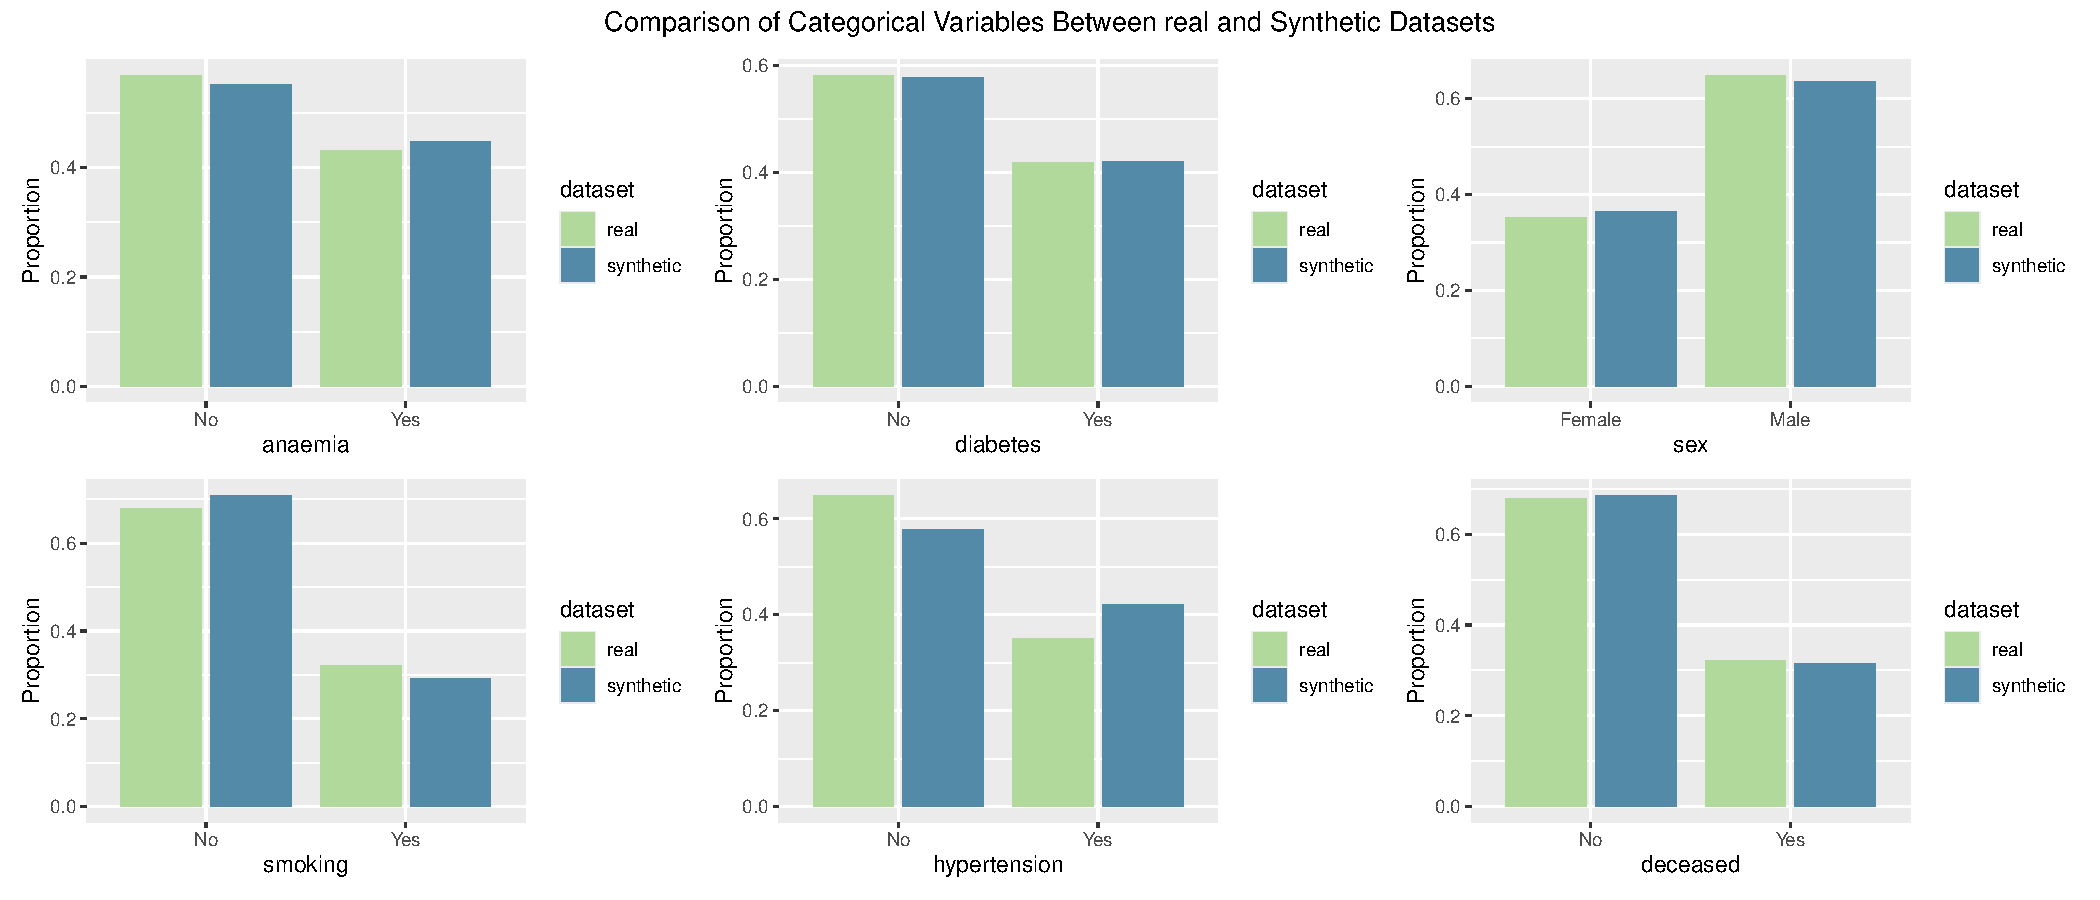
\includegraphics[width=1\linewidth,height=\textheight,keepaspectratio]{heart_failure_synthetic_data_project_files/figure-pdf/Bar Plots for Categorical Variables-1.pdf}
\end{center}

\subparagraph{Density Plots for Numeric
Variables}\label{density-plots-for-numeric-variables}

The density plots illustrate the distribution of numeric variables
between the real dataset and the parametric MICE synthetic data. The
goal is to ensure that the synthetic data closely follows the real
data's numeric distribution.

\begin{Shaded}
\begin{Highlighting}[]
\CommentTok{\# Density plots for numeric variables (parametric imputed data)}
\NormalTok{density\_plots\_param }\OtherTok{\textless{}{-}} \FunctionTok{colnames}\NormalTok{(heart\_failure)[}\FunctionTok{map\_lgl}\NormalTok{(heart\_failure, is.numeric)] }\SpecialCharTok{\%\textgreater{}\%}
  \FunctionTok{map}\NormalTok{(}\SpecialCharTok{\textasciitilde{}} \FunctionTok{ggplot}\NormalTok{(combined\_data\_param, }\FunctionTok{aes\_string}\NormalTok{(.x, }\AttributeTok{fill =} \StringTok{\textquotesingle{}dataset\textquotesingle{}}\NormalTok{, }\AttributeTok{group =} \StringTok{\textquotesingle{}dataset\textquotesingle{}}\NormalTok{)) }\SpecialCharTok{+}
        \FunctionTok{geom\_density}\NormalTok{(}\AttributeTok{alpha =} \FloatTok{0.5}\NormalTok{) }\SpecialCharTok{+}
        \FunctionTok{scale\_fill\_manual}\NormalTok{(}\AttributeTok{values =} \FunctionTok{c}\NormalTok{(}\StringTok{"real"} \OtherTok{=} \StringTok{"\#B0D99B"}\NormalTok{, }\StringTok{"synthetic"} \OtherTok{=} \StringTok{"\#528AA8"}\NormalTok{)) }\SpecialCharTok{+}
        \FunctionTok{labs}\NormalTok{(}\AttributeTok{x =}\NormalTok{ .x, }\AttributeTok{y =} \StringTok{"Density"}\NormalTok{)) }\SpecialCharTok{\%\textgreater{}\%}
\NormalTok{  patchwork}\SpecialCharTok{::}\FunctionTok{wrap\_plots}\NormalTok{(}\AttributeTok{ncol =} \DecValTok{2}\NormalTok{) }\SpecialCharTok{+}  \CommentTok{\# Arrange plots in 2 columns}
  \FunctionTok{plot\_annotation}\NormalTok{(}\AttributeTok{title =} \StringTok{"Comparison of Numeric Variables Between real and Parametric Synthetic Data"}\NormalTok{,}
                  \AttributeTok{theme =} \FunctionTok{theme}\NormalTok{(}\AttributeTok{plot.title =} \FunctionTok{element\_text}\NormalTok{(}\AttributeTok{hjust =} \FloatTok{0.5}\NormalTok{)))}

\CommentTok{\# Print the combined density plots with one main title}
\FunctionTok{print}\NormalTok{(density\_plots\_param)}
\end{Highlighting}
\end{Shaded}

\begin{center}
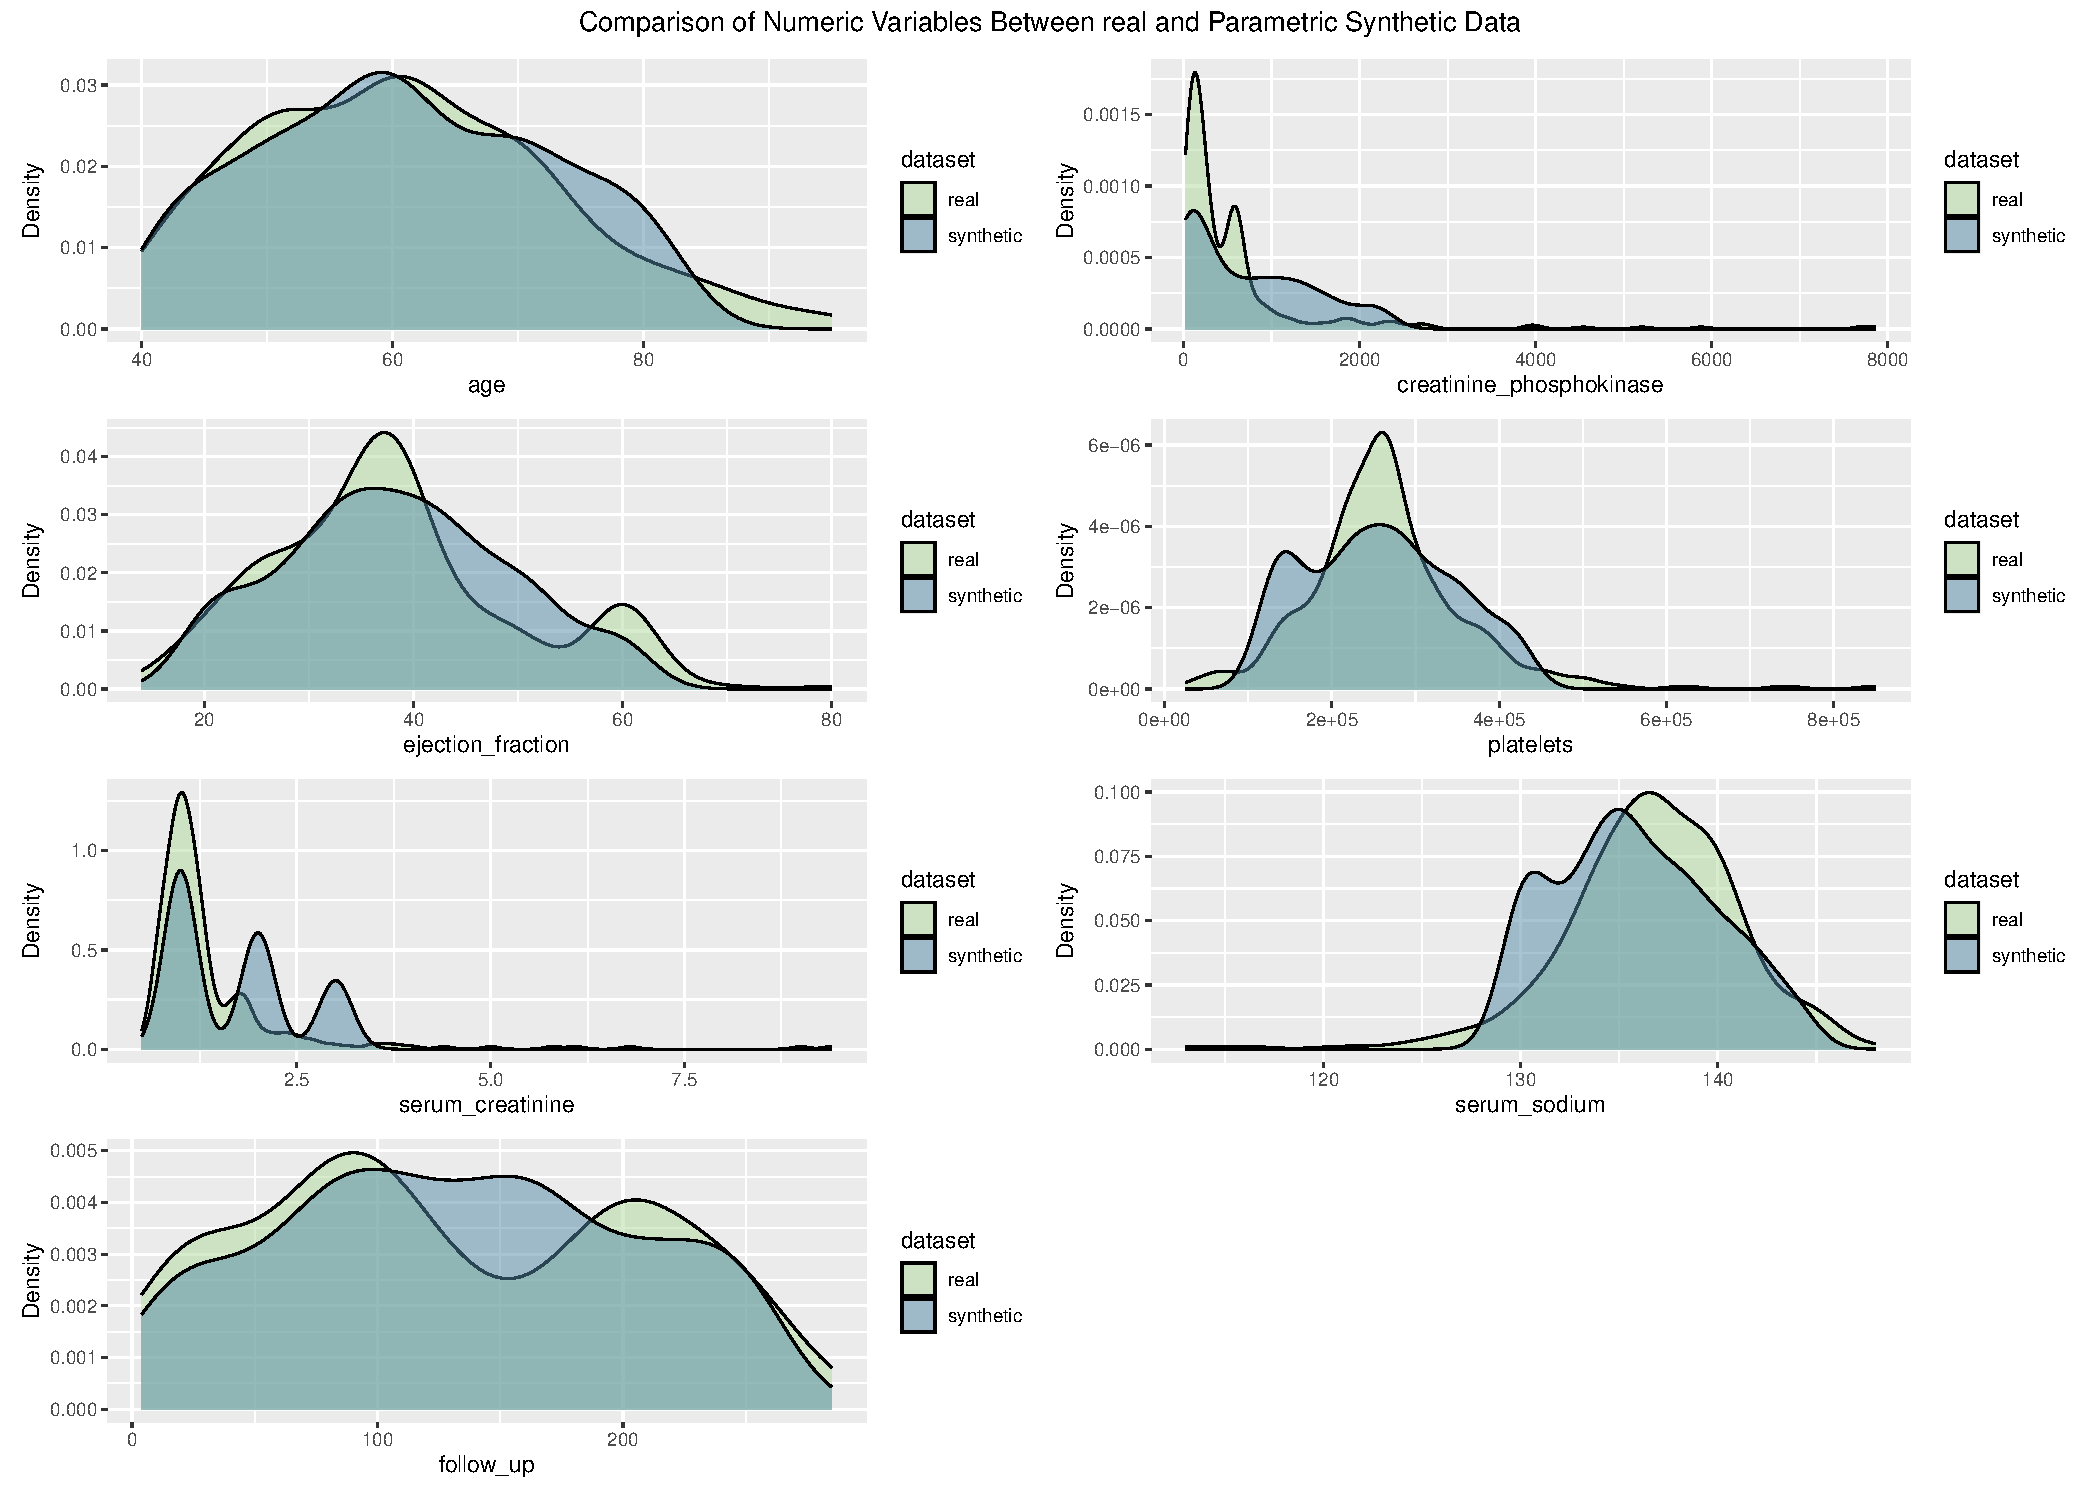
\includegraphics[width=1\linewidth,height=\textheight,keepaspectratio]{heart_failure_synthetic_data_project_files/figure-pdf/Density plots for numeric variables (parametric imputed data)-1.pdf}
\end{center}

\paragraph{Non-Parametric Imputation
(CART)}\label{non-parametric-imputation-cart-1}

CART is a non-parametric approach for generating synthetic data that
captures complex relationships between variables without making
distributional assumptions.

\subparagraph{Bar Plots for Categorical
Variables}\label{bar-plots-for-categorical-variables-1}

The bar plots compare the distribution of categorical variables in the
real and synthetic datasets generated using the CART method.

\begin{Shaded}
\begin{Highlighting}[]
\CommentTok{\# Combine real and non{-}parametric CART synthetic datasets}
\NormalTok{syn\_cart\_1}\SpecialCharTok{$}\NormalTok{dataset }\OtherTok{\textless{}{-}} \StringTok{"synthetic"}

\CommentTok{\# Adjust the column names for synthetic data by removing the \textquotesingle{}synth\_\textquotesingle{} prefix}
\FunctionTok{colnames}\NormalTok{(syn\_cart\_1) }\OtherTok{\textless{}{-}} \FunctionTok{gsub}\NormalTok{(}\StringTok{"synth\_"}\NormalTok{, }\StringTok{""}\NormalTok{, }\FunctionTok{colnames}\NormalTok{(syn\_cart\_1))}

\CommentTok{\# Combine both datasets (real and synthetic)}
\NormalTok{combined\_data\_cart }\OtherTok{\textless{}{-}} \FunctionTok{bind\_rows}\NormalTok{(heart\_failure, syn\_cart\_1)}

\CommentTok{\# Bar plots for categorical variables (CART{-}imputed data)}
\NormalTok{bar\_plots\_cart }\OtherTok{\textless{}{-}} \FunctionTok{colnames}\NormalTok{(heart\_failure)[}\FunctionTok{map\_lgl}\NormalTok{(heart\_failure, is.factor)] }\SpecialCharTok{\%\textgreater{}\%}
  \FunctionTok{map}\NormalTok{(}\SpecialCharTok{\textasciitilde{}} \FunctionTok{ggplot}\NormalTok{(combined\_data\_cart, }\FunctionTok{aes\_string}\NormalTok{(.x, }\AttributeTok{fill =} \StringTok{\textquotesingle{}dataset\textquotesingle{}}\NormalTok{, }\AttributeTok{group =} \StringTok{\textquotesingle{}dataset\textquotesingle{}}\NormalTok{)) }\SpecialCharTok{+}
        \FunctionTok{geom\_bar}\NormalTok{(}\FunctionTok{aes}\NormalTok{(}\AttributeTok{y =}\NormalTok{ ..prop..), }\AttributeTok{position =} \FunctionTok{position\_dodge2}\NormalTok{(), }\AttributeTok{stat =} \StringTok{"count"}\NormalTok{) }\SpecialCharTok{+}
        \FunctionTok{scale\_fill\_manual}\NormalTok{(}\AttributeTok{values =} \FunctionTok{c}\NormalTok{(}\StringTok{"real"} \OtherTok{=} \StringTok{"\#B0D99B"}\NormalTok{, }\StringTok{"synthetic"} \OtherTok{=} \StringTok{"\#528AA8"}\NormalTok{)) }\SpecialCharTok{+}
        \FunctionTok{labs}\NormalTok{(}\AttributeTok{x =}\NormalTok{ .x, }\AttributeTok{y =} \StringTok{"Proportion"}\NormalTok{)) }\SpecialCharTok{\%\textgreater{}\%}
\NormalTok{  patchwork}\SpecialCharTok{::}\FunctionTok{wrap\_plots}\NormalTok{() }\SpecialCharTok{+}
  \FunctionTok{plot\_annotation}\NormalTok{(}\AttributeTok{title =} \StringTok{"Comparison of Categorical Variables Between real and Synthetic Data"}\NormalTok{,}
                  \AttributeTok{theme =} \FunctionTok{theme}\NormalTok{(}\AttributeTok{plot.title =} \FunctionTok{element\_text}\NormalTok{(}\AttributeTok{hjust =} \FloatTok{0.5}\NormalTok{)))}

\CommentTok{\# Print the combined plot with one main title}
\FunctionTok{print}\NormalTok{(bar\_plots\_cart)}
\end{Highlighting}
\end{Shaded}

\begin{center}
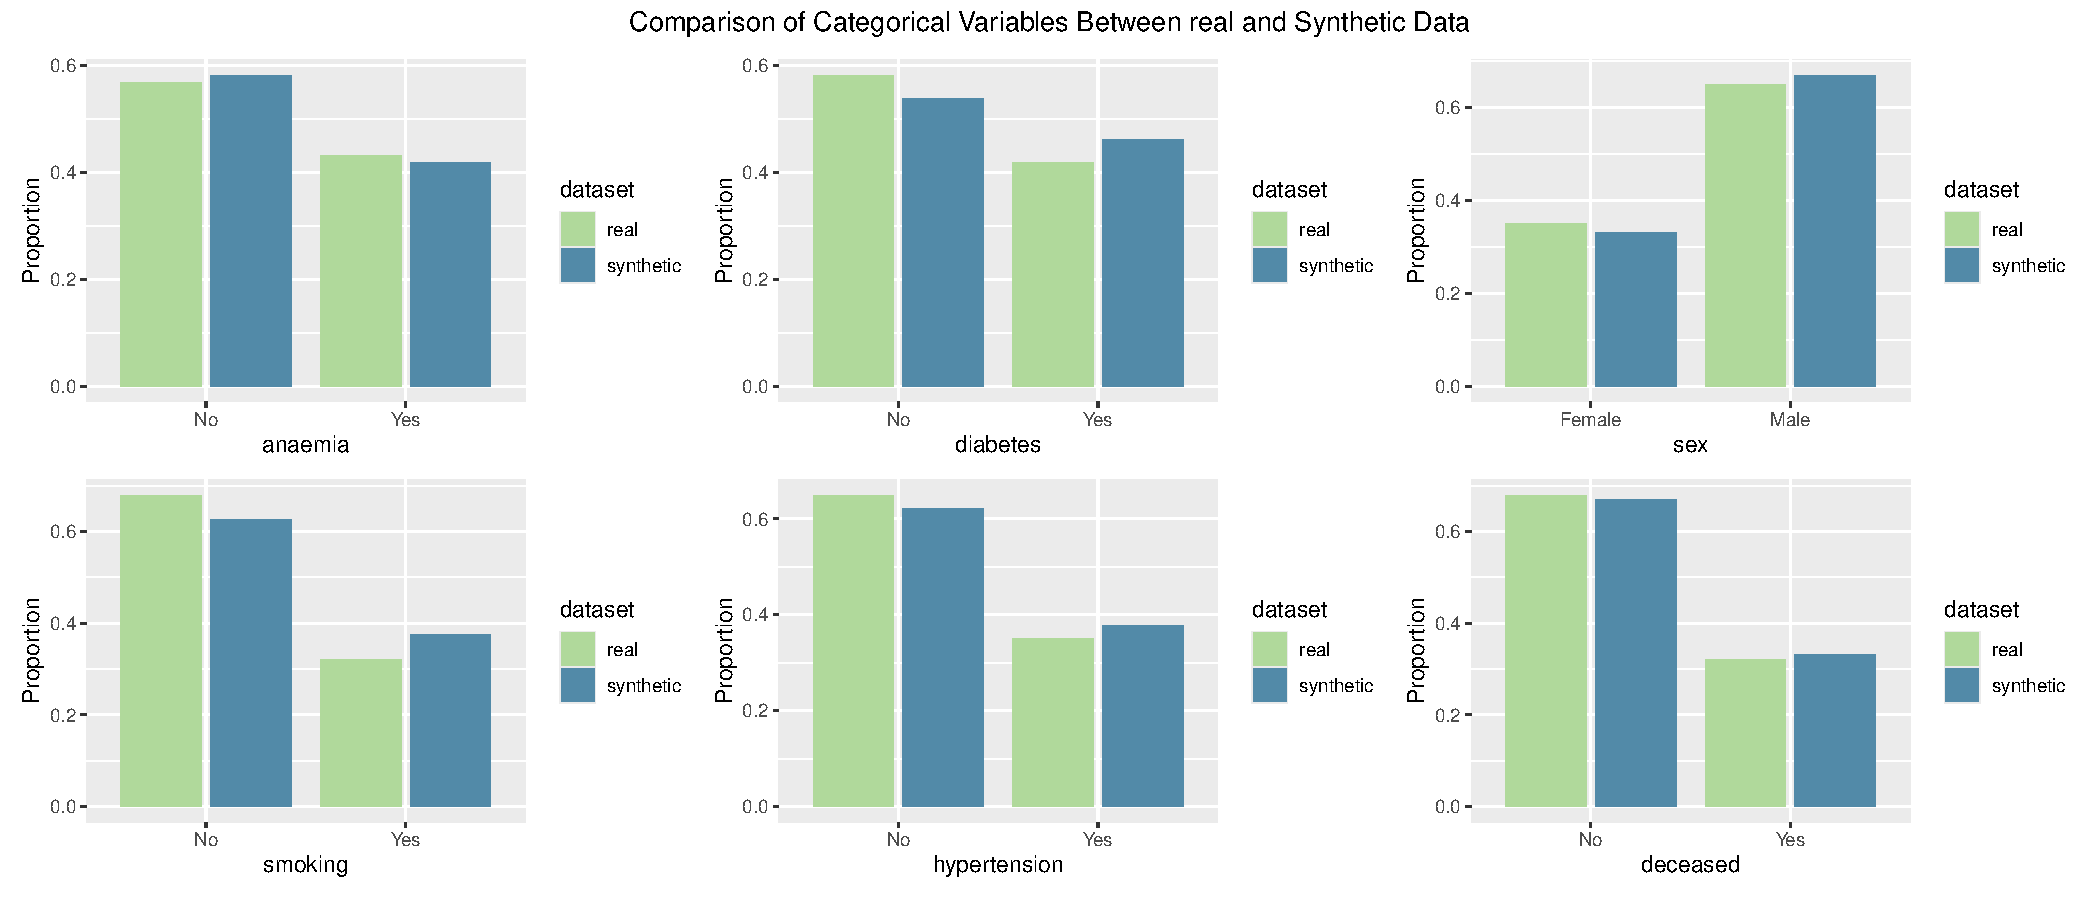
\includegraphics[width=1\linewidth,height=\textheight,keepaspectratio]{heart_failure_synthetic_data_project_files/figure-pdf/Bar plots for categorical variables (CART-imputed data)-1.pdf}
\end{center}

\subparagraph{Density Plots for Numeric
Variables}\label{density-plots-for-numeric-variables-1}

The density plots display how well the numeric variables in the
CART-imputed synthetic data align with the real dataset.

\begin{Shaded}
\begin{Highlighting}[]
\CommentTok{\# Density plots for numeric variables (CART{-}imputed data)}
\NormalTok{density\_plots\_cart }\OtherTok{\textless{}{-}} \FunctionTok{colnames}\NormalTok{(heart\_failure)[}\FunctionTok{map\_lgl}\NormalTok{(heart\_failure, is.numeric)] }\SpecialCharTok{\%\textgreater{}\%}
  \FunctionTok{map}\NormalTok{(}\SpecialCharTok{\textasciitilde{}} \FunctionTok{ggplot}\NormalTok{(combined\_data\_cart, }\FunctionTok{aes\_string}\NormalTok{(.x, }\AttributeTok{fill =} \StringTok{\textquotesingle{}dataset\textquotesingle{}}\NormalTok{, }\AttributeTok{group =} \StringTok{\textquotesingle{}dataset\textquotesingle{}}\NormalTok{)) }\SpecialCharTok{+}
        \FunctionTok{geom\_density}\NormalTok{(}\AttributeTok{alpha =} \FloatTok{0.5}\NormalTok{) }\SpecialCharTok{+}
        \FunctionTok{scale\_fill\_manual}\NormalTok{(}\AttributeTok{values =} \FunctionTok{c}\NormalTok{(}\StringTok{"real"} \OtherTok{=} \StringTok{"\#B0D99B"}\NormalTok{, }\StringTok{"synthetic"} \OtherTok{=} \StringTok{"\#528AA8"}\NormalTok{)) }\SpecialCharTok{+}
        \FunctionTok{labs}\NormalTok{(}\AttributeTok{x =}\NormalTok{ .x, }\AttributeTok{y =} \StringTok{"Density"}\NormalTok{)) }\SpecialCharTok{\%\textgreater{}\%}
\NormalTok{  patchwork}\SpecialCharTok{::}\FunctionTok{wrap\_plots}\NormalTok{(}\AttributeTok{ncol =} \DecValTok{2}\NormalTok{) }\SpecialCharTok{+}  \CommentTok{\# Arrange plots in 2 columns}
  \FunctionTok{plot\_annotation}\NormalTok{(}\AttributeTok{title =} \StringTok{"Comparison of Numeric Variables Between real and Synthetic Data"}\NormalTok{,}
                  \AttributeTok{theme =} \FunctionTok{theme}\NormalTok{(}\AttributeTok{plot.title =} \FunctionTok{element\_text}\NormalTok{(}\AttributeTok{hjust =} \FloatTok{0.5}\NormalTok{)))}

\CommentTok{\# Print the combined density plots with one main title}
\FunctionTok{print}\NormalTok{(density\_plots\_cart)}
\end{Highlighting}
\end{Shaded}

\begin{center}
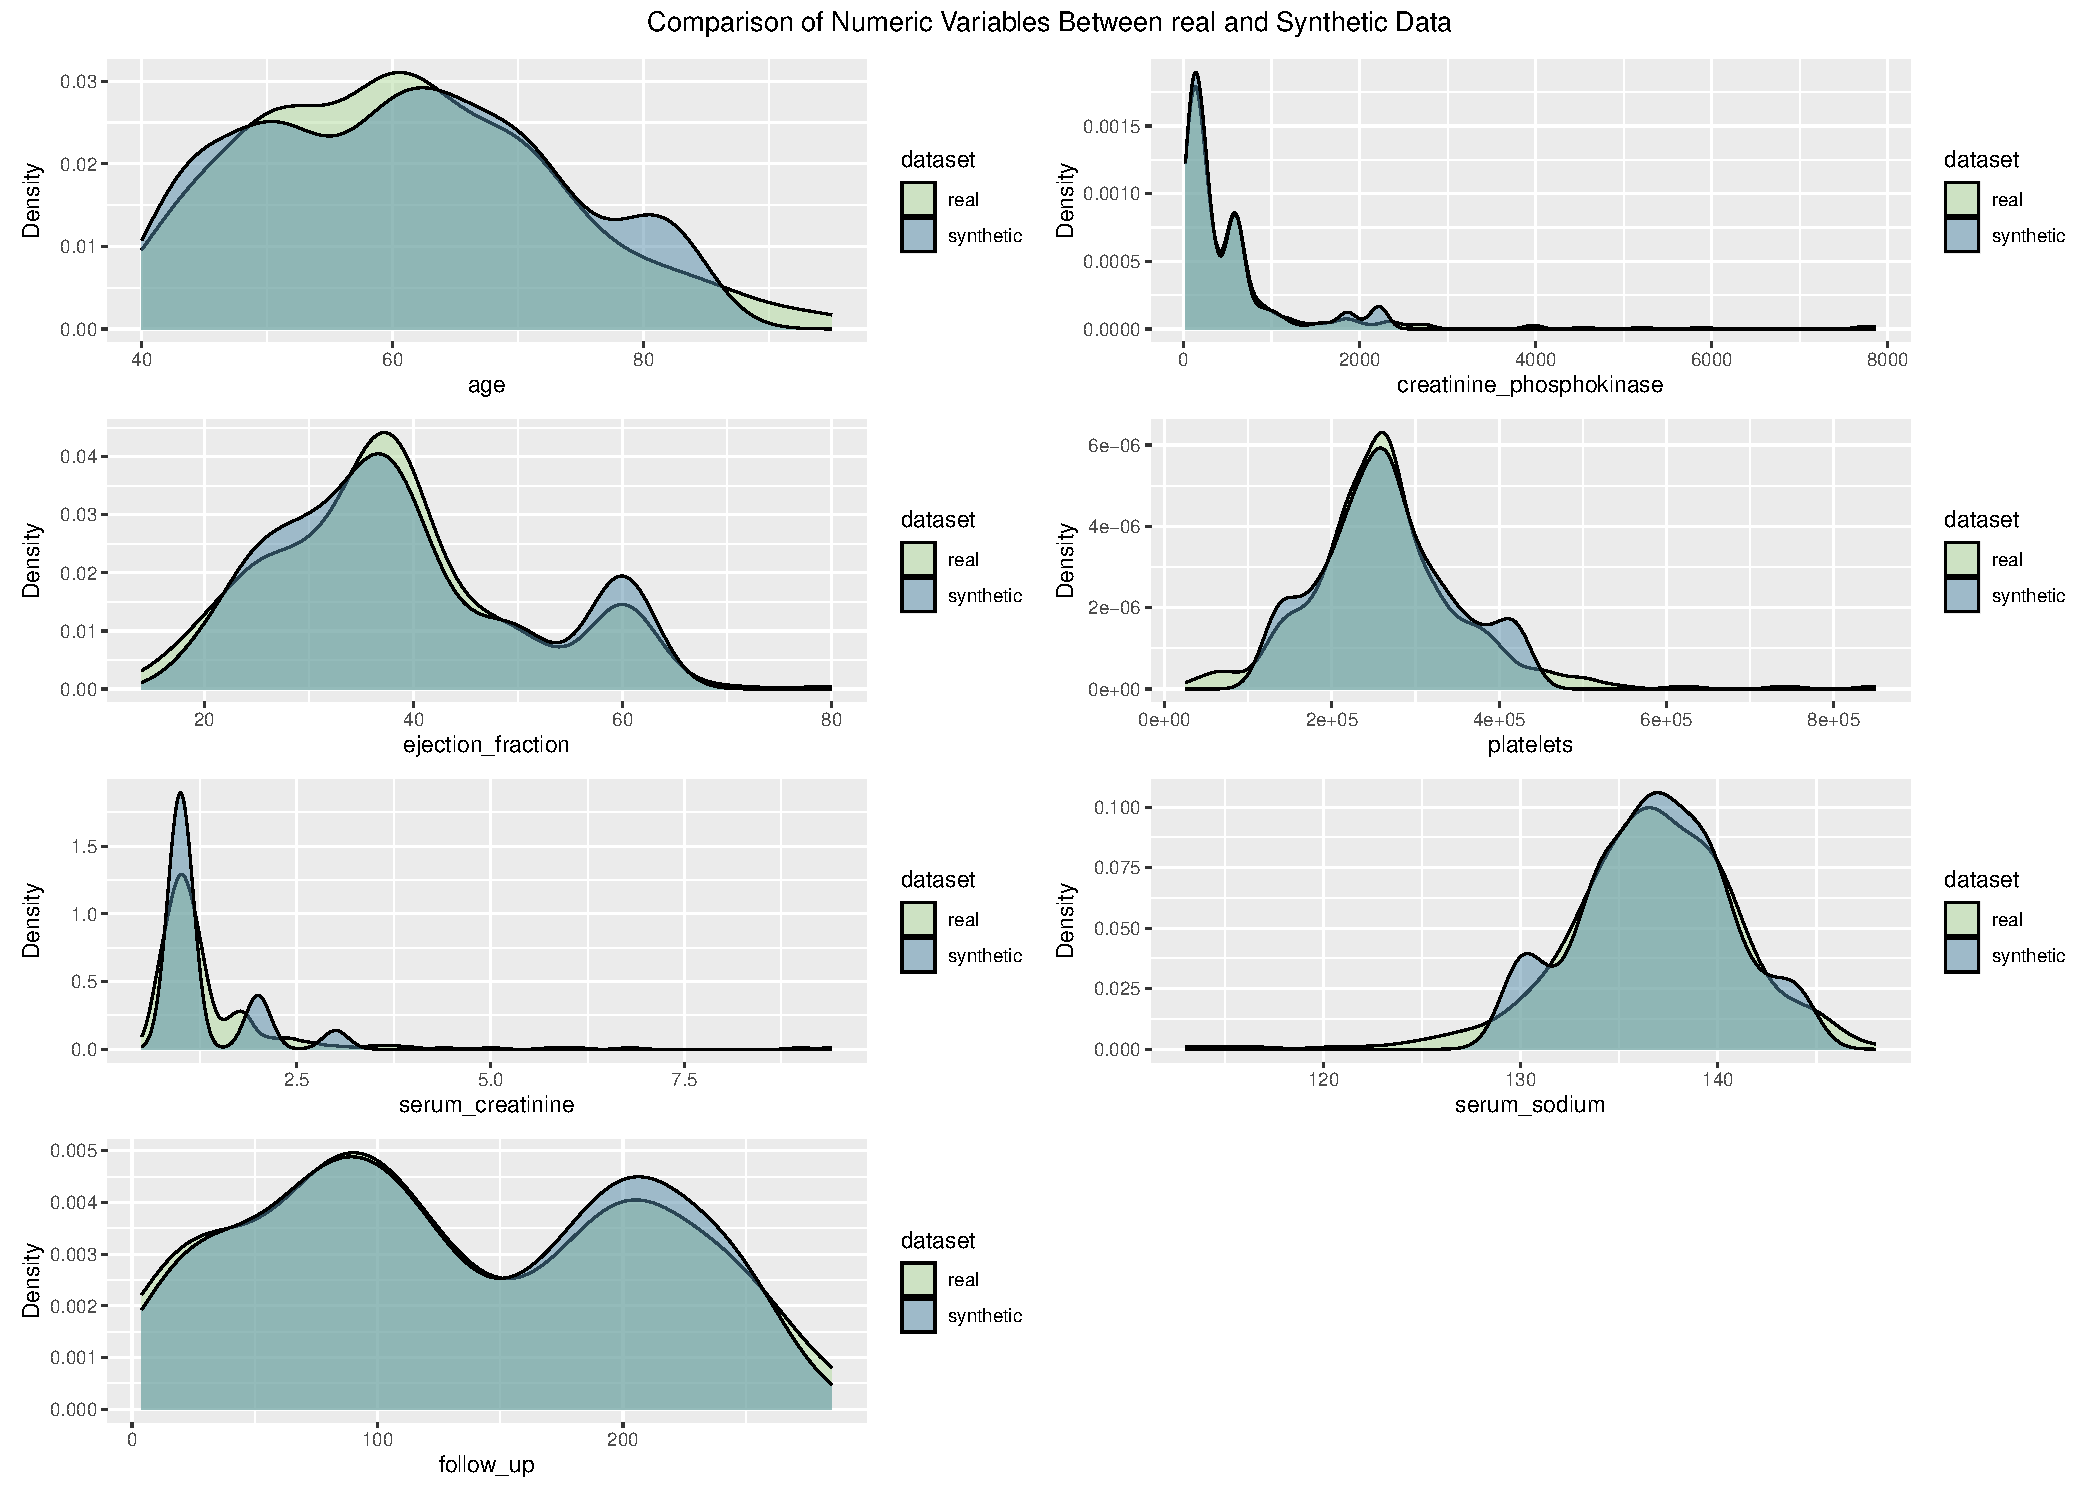
\includegraphics[width=1\linewidth,height=\textheight,keepaspectratio]{heart_failure_synthetic_data_project_files/figure-pdf/Density plots for numeric variables (CART-imputed data)-1.pdf}
\end{center}

\paragraph{Synthpop-Based Synthetic
Data}\label{synthpop-based-synthetic-data-1}

Synthpop is used to generate synthetic datasets that closely follow the
distributions of the real data for privacy-preserving data sharing.

\subparagraph{Bar Plots for Categorical
Variables}\label{bar-plots-for-categorical-variables-2}

These bar plots assess how well Synthpop-based synthetic data maintains
the categorical distributions of the real dataset.

\begin{Shaded}
\begin{Highlighting}[]
\CommentTok{\# Combine real and Synthpop{-}based synthetic datasets}
\NormalTok{heart\_failure}\SpecialCharTok{$}\NormalTok{dataset }\OtherTok{\textless{}{-}} \StringTok{"real"}
\NormalTok{syn\_data\_low\_fidelity\_synthpop}\SpecialCharTok{$}\NormalTok{dataset }\OtherTok{\textless{}{-}} \StringTok{"synthetic"}

\CommentTok{\# Adjust the column names for synthetic data by removing the \textquotesingle{}synth\_\textquotesingle{} prefix}
\FunctionTok{colnames}\NormalTok{(syn\_data\_low\_fidelity\_synthpop) }\OtherTok{\textless{}{-}} \FunctionTok{gsub}\NormalTok{(}\StringTok{"synth\_"}\NormalTok{, }\StringTok{""}\NormalTok{, }\FunctionTok{colnames}\NormalTok{(syn\_data\_low\_fidelity\_synthpop))}

\CommentTok{\# Combine both datasets (real and synthetic)}
\NormalTok{combined\_data\_synthpop }\OtherTok{\textless{}{-}} \FunctionTok{bind\_rows}\NormalTok{(heart\_failure, syn\_data\_low\_fidelity\_synthpop)}

\CommentTok{\# Bar plots for categorical variables (Synthpop{-}based synthetic data)}
\NormalTok{bar\_plots\_synthpop }\OtherTok{\textless{}{-}} \FunctionTok{colnames}\NormalTok{(heart\_failure)[}\FunctionTok{map\_lgl}\NormalTok{(heart\_failure, is.factor)] }\SpecialCharTok{\%\textgreater{}\%}
  \FunctionTok{map}\NormalTok{(}\SpecialCharTok{\textasciitilde{}} \FunctionTok{ggplot}\NormalTok{(combined\_data\_synthpop, }\FunctionTok{aes\_string}\NormalTok{(.x, }\AttributeTok{fill =} \StringTok{\textquotesingle{}dataset\textquotesingle{}}\NormalTok{, }\AttributeTok{group =} \StringTok{\textquotesingle{}dataset\textquotesingle{}}\NormalTok{)) }\SpecialCharTok{+}
        \FunctionTok{geom\_bar}\NormalTok{(}\FunctionTok{aes}\NormalTok{(}\AttributeTok{y =}\NormalTok{ ..prop..), }\AttributeTok{position =} \FunctionTok{position\_dodge2}\NormalTok{(), }\AttributeTok{stat =} \StringTok{"count"}\NormalTok{) }\SpecialCharTok{+}
        \FunctionTok{scale\_fill\_manual}\NormalTok{(}\AttributeTok{values =} \FunctionTok{c}\NormalTok{(}\StringTok{"real"} \OtherTok{=} \StringTok{"\#B0D99B"}\NormalTok{, }\StringTok{"synthetic"} \OtherTok{=} \StringTok{"\#528AA8"}\NormalTok{)) }\SpecialCharTok{+}
        \FunctionTok{labs}\NormalTok{(}\AttributeTok{x =}\NormalTok{ .x, }\AttributeTok{y =} \StringTok{"Proportion"}\NormalTok{)) }\SpecialCharTok{\%\textgreater{}\%}
\NormalTok{  patchwork}\SpecialCharTok{::}\FunctionTok{wrap\_plots}\NormalTok{() }\SpecialCharTok{+}
  \FunctionTok{plot\_annotation}\NormalTok{(}\AttributeTok{title =} \StringTok{"Comparison of Categorical Variables Between real and Synthetic Data"}\NormalTok{,}
                  \AttributeTok{theme =} \FunctionTok{theme}\NormalTok{(}\AttributeTok{plot.title =} \FunctionTok{element\_text}\NormalTok{(}\AttributeTok{hjust =} \FloatTok{0.5}\NormalTok{)))}

\CommentTok{\# Print the combined plot with one main title}
\FunctionTok{print}\NormalTok{(bar\_plots\_synthpop)}
\end{Highlighting}
\end{Shaded}

\begin{center}
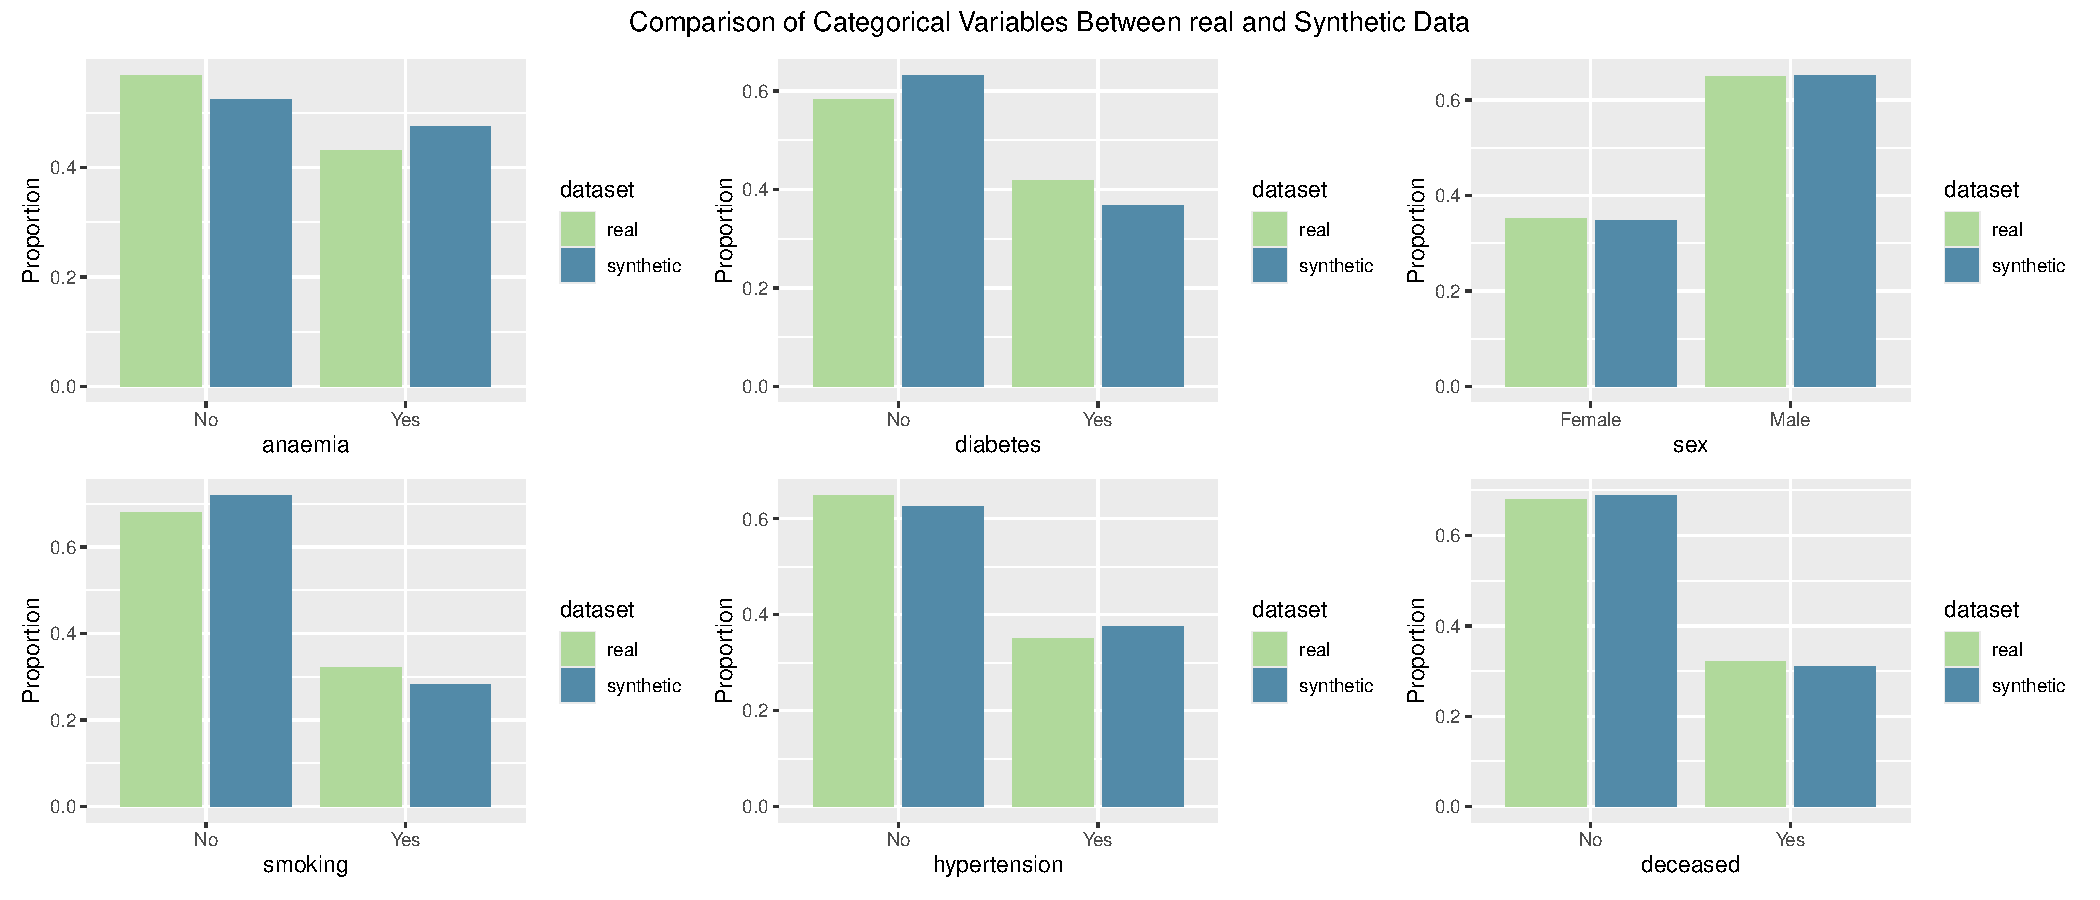
\includegraphics[width=1\linewidth,height=\textheight,keepaspectratio]{heart_failure_synthetic_data_project_files/figure-pdf/Bar plots for categorical variables (Synthpop-based synthetic data)-1.pdf}
\end{center}

\subparagraph{Density Plots for Numeric
Variables}\label{density-plots-for-numeric-variables-2}

The density plots illustrate how closely Synthpop-based synthetic data
matches the real dataset for numeric variables.

\begin{Shaded}
\begin{Highlighting}[]
\CommentTok{\# Combine real and Synthpop{-}based synthetic datasets}
\NormalTok{heart\_failure}\SpecialCharTok{$}\NormalTok{dataset }\OtherTok{\textless{}{-}} \StringTok{"real"}
\NormalTok{syn\_data\_low\_fidelity\_synthpop}\SpecialCharTok{$}\NormalTok{dataset }\OtherTok{\textless{}{-}} \StringTok{"synthetic"}
\NormalTok{combined\_data\_synthpop }\OtherTok{\textless{}{-}} \FunctionTok{bind\_rows}\NormalTok{(heart\_failure, syn\_data\_low\_fidelity\_synthpop)}

\CommentTok{\# Density plots for numeric variables (Synthpop{-}based synthetic data)}
\NormalTok{density\_plots\_synthpop }\OtherTok{\textless{}{-}} \FunctionTok{colnames}\NormalTok{(heart\_failure)[}\FunctionTok{map\_lgl}\NormalTok{(heart\_failure, is.numeric)] }\SpecialCharTok{\%\textgreater{}\%}
  \FunctionTok{map}\NormalTok{(}\SpecialCharTok{\textasciitilde{}} \FunctionTok{ggplot}\NormalTok{(combined\_data\_synthpop, }\FunctionTok{aes\_string}\NormalTok{(.x, }\AttributeTok{fill =} \StringTok{\textquotesingle{}dataset\textquotesingle{}}\NormalTok{, }\AttributeTok{group =} \StringTok{\textquotesingle{}dataset\textquotesingle{}}\NormalTok{)) }\SpecialCharTok{+}
        \FunctionTok{geom\_density}\NormalTok{(}\AttributeTok{alpha =} \FloatTok{0.5}\NormalTok{) }\SpecialCharTok{+}
        \FunctionTok{scale\_fill\_manual}\NormalTok{(}\AttributeTok{values =} \FunctionTok{c}\NormalTok{(}\StringTok{"real"} \OtherTok{=} \StringTok{"\#B0D99B"}\NormalTok{, }\StringTok{"synthetic"} \OtherTok{=} \StringTok{"\#528AA8"}\NormalTok{)) }\SpecialCharTok{+}
        \FunctionTok{labs}\NormalTok{(}\AttributeTok{x =}\NormalTok{ .x, }\AttributeTok{y =} \StringTok{"Density"}\NormalTok{)) }\SpecialCharTok{\%\textgreater{}\%}
\NormalTok{  patchwork}\SpecialCharTok{::}\FunctionTok{wrap\_plots}\NormalTok{(}\AttributeTok{ncol =} \DecValTok{2}\NormalTok{) }\SpecialCharTok{+}  \CommentTok{\# Arrange plots in 2 columns}
  \FunctionTok{plot\_annotation}\NormalTok{(}\AttributeTok{title =} \StringTok{"Comparison of Numeric Variables Between real and Synthetic Data"}\NormalTok{,}
                  \AttributeTok{theme =} \FunctionTok{theme}\NormalTok{(}\AttributeTok{plot.title =} \FunctionTok{element\_text}\NormalTok{(}\AttributeTok{hjust =} \FloatTok{0.5}\NormalTok{)))}

\CommentTok{\# Print the combined density plots with one main title}
\FunctionTok{print}\NormalTok{(density\_plots\_synthpop)}
\end{Highlighting}
\end{Shaded}

\begin{center}
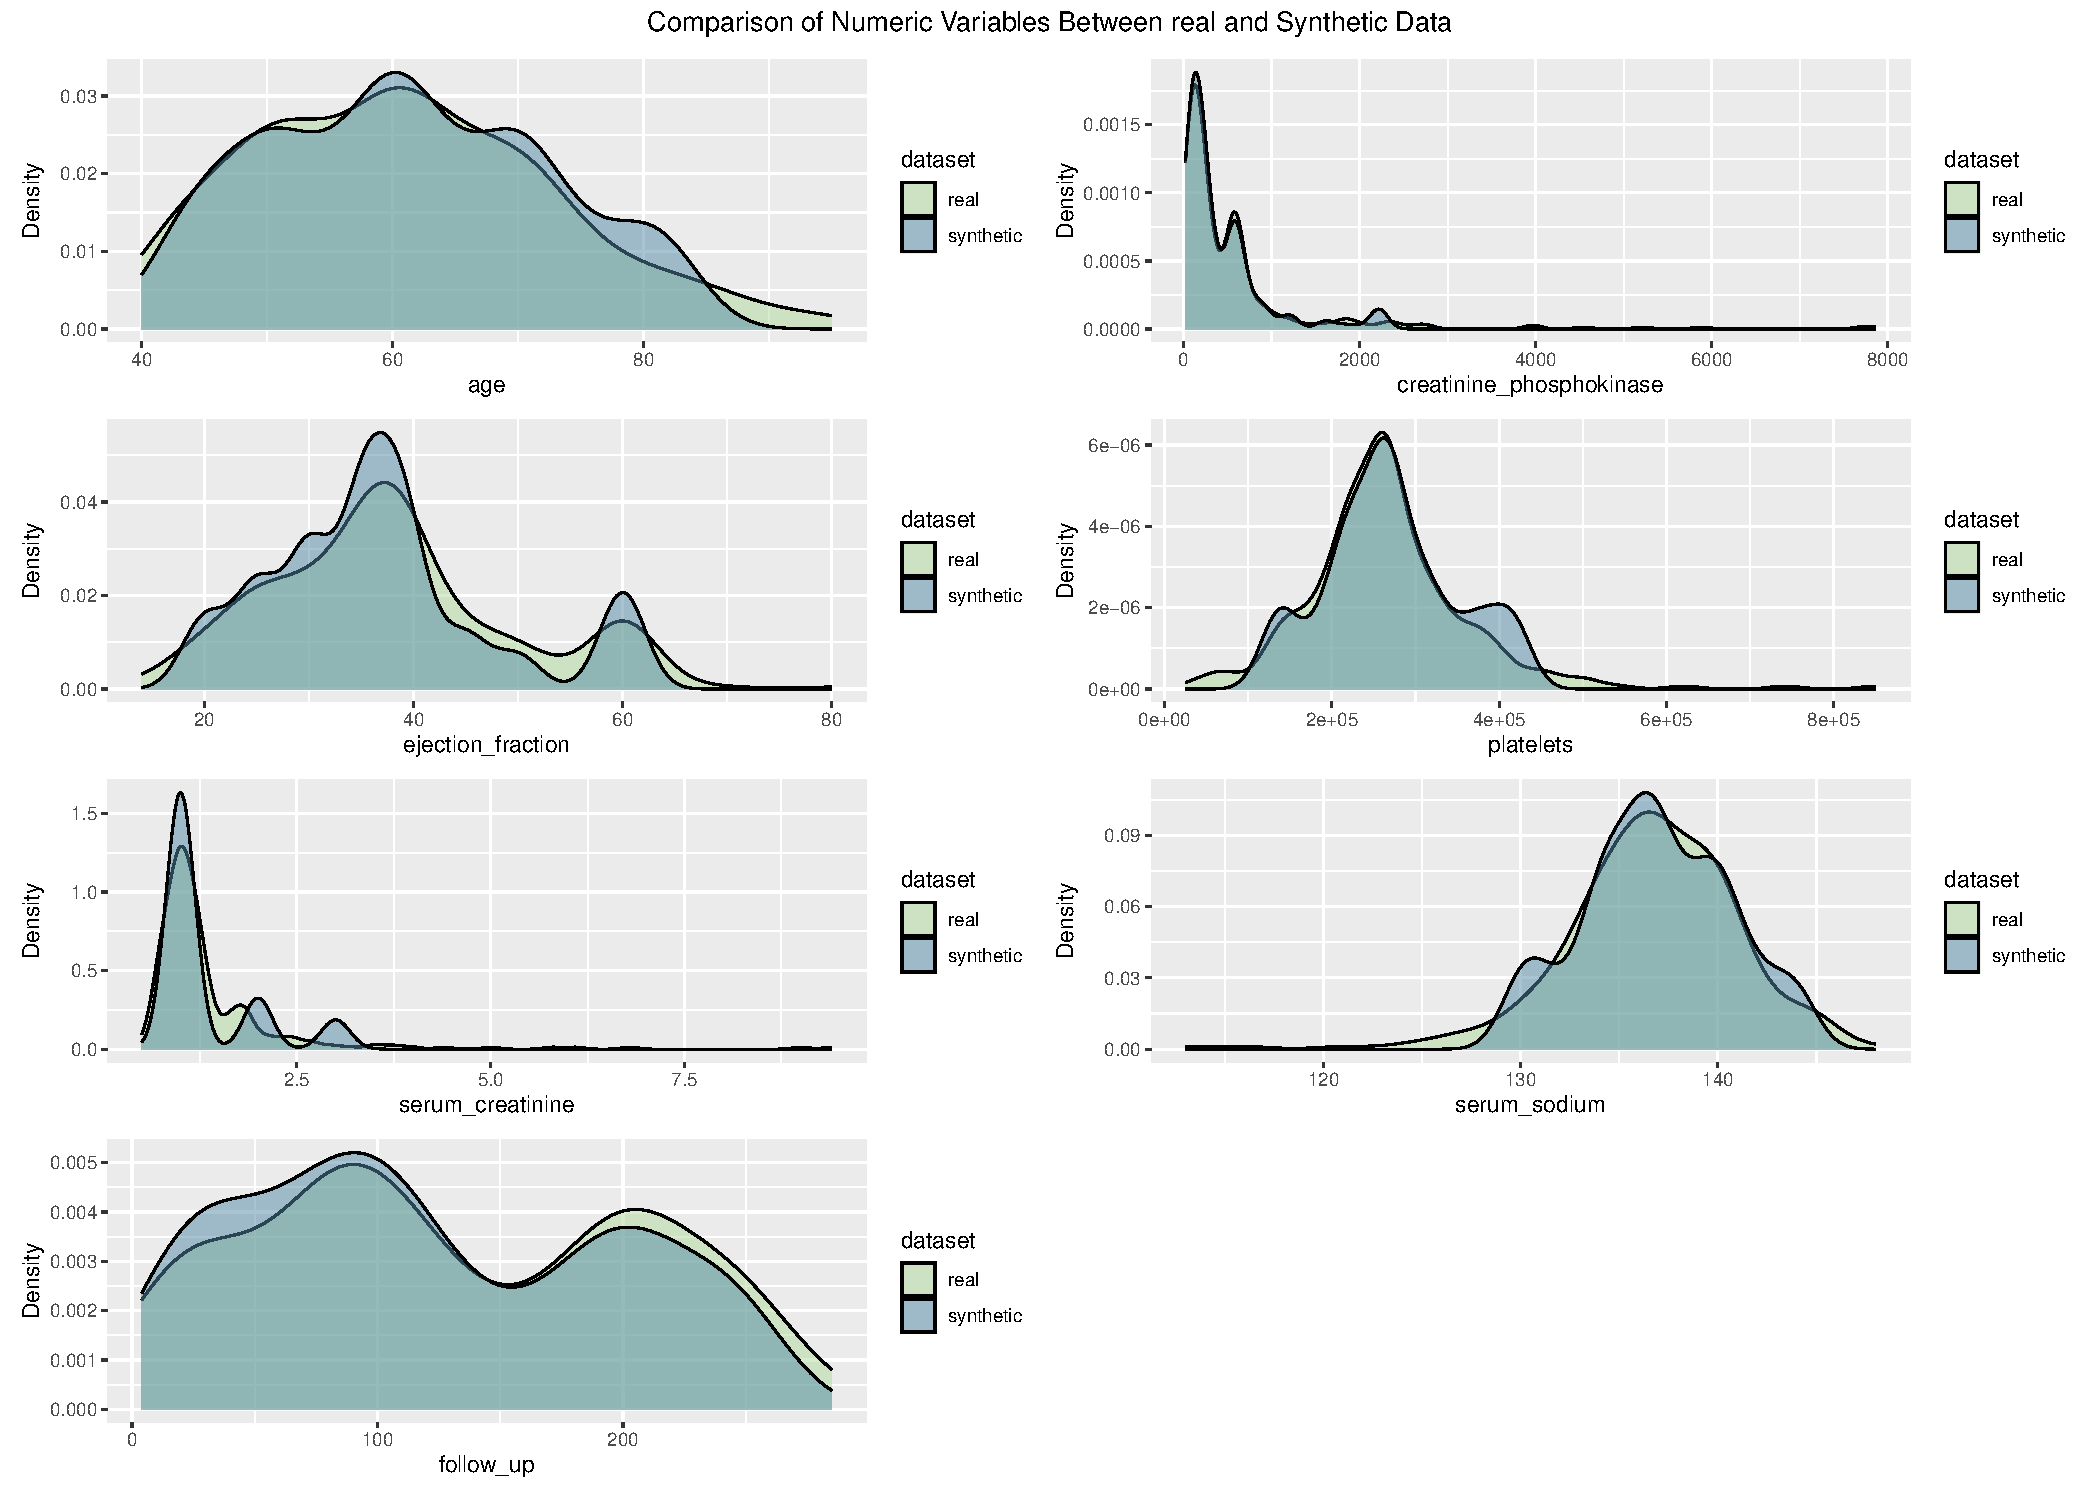
\includegraphics[width=1\linewidth,height=\textheight,keepaspectratio]{heart_failure_synthetic_data_project_files/figure-pdf/Density plots for numeric variables (Synthpop-based synthetic data)-1.pdf}
\end{center}

\paragraph{Metadata-Based Synthetic
Data}\label{metadata-based-synthetic-data-1}

Metadata-based synthetic data generation uses a predefined data
dictionary to ensure that the synthetic data follows the correct
structure and distribution.

\subparagraph{Bar Plots for Categorical
Variables}\label{bar-plots-for-categorical-variables-3}

We compare the categorical variables of the real and metadata-based
synthetic datasets to assess distributional alignment.

\begin{Shaded}
\begin{Highlighting}[]
\CommentTok{\# Combine real and Metadata{-}based synthetic datasets}
\NormalTok{heart\_failure}\SpecialCharTok{$}\NormalTok{dataset }\OtherTok{\textless{}{-}} \StringTok{"real"}
\NormalTok{syn\_data\_metadata}\SpecialCharTok{$}\NormalTok{dataset }\OtherTok{\textless{}{-}} \StringTok{"synthetic"}

\CommentTok{\# Adjust the column names for synthetic data by removing the \textquotesingle{}synth\_\textquotesingle{} prefix}
\FunctionTok{colnames}\NormalTok{(syn\_data\_metadata) }\OtherTok{\textless{}{-}} \FunctionTok{gsub}\NormalTok{(}\StringTok{"synth\_"}\NormalTok{, }\StringTok{""}\NormalTok{, }\FunctionTok{colnames}\NormalTok{(syn\_data\_metadata))}

\CommentTok{\# Combine both datasets (real and synthetic)}
\NormalTok{combined\_data\_metadata }\OtherTok{\textless{}{-}} \FunctionTok{bind\_rows}\NormalTok{(heart\_failure, syn\_data\_metadata)}

\CommentTok{\# Bar plots for categorical variables (Metadata{-}based synthetic data)}
\NormalTok{bar\_plots\_metadata }\OtherTok{\textless{}{-}} \FunctionTok{colnames}\NormalTok{(heart\_failure)[}\FunctionTok{map\_lgl}\NormalTok{(heart\_failure, is.factor)] }\SpecialCharTok{\%\textgreater{}\%}
  \FunctionTok{map}\NormalTok{(}\SpecialCharTok{\textasciitilde{}} \FunctionTok{ggplot}\NormalTok{(combined\_data\_metadata, }\FunctionTok{aes\_string}\NormalTok{(.x, }\AttributeTok{fill =} \StringTok{\textquotesingle{}dataset\textquotesingle{}}\NormalTok{, }\AttributeTok{group =} \StringTok{\textquotesingle{}dataset\textquotesingle{}}\NormalTok{)) }\SpecialCharTok{+}
        \FunctionTok{geom\_bar}\NormalTok{(}\FunctionTok{aes}\NormalTok{(}\AttributeTok{y =}\NormalTok{ ..prop..), }\AttributeTok{position =} \FunctionTok{position\_dodge2}\NormalTok{(), }\AttributeTok{stat =} \StringTok{"count"}\NormalTok{) }\SpecialCharTok{+}
        \FunctionTok{scale\_fill\_manual}\NormalTok{(}\AttributeTok{values =} \FunctionTok{c}\NormalTok{(}\StringTok{"real"} \OtherTok{=} \StringTok{"\#B0D99B"}\NormalTok{, }\StringTok{"synthetic"} \OtherTok{=} \StringTok{"\#528AA8"}\NormalTok{)) }\SpecialCharTok{+}
        \FunctionTok{labs}\NormalTok{(}\AttributeTok{x =}\NormalTok{ .x, }\AttributeTok{y =} \StringTok{"Proportion"}\NormalTok{)) }\SpecialCharTok{\%\textgreater{}\%}
\NormalTok{  patchwork}\SpecialCharTok{::}\FunctionTok{wrap\_plots}\NormalTok{() }\SpecialCharTok{+}
  \FunctionTok{plot\_annotation}\NormalTok{(}\AttributeTok{title =} \StringTok{"Comparison of Categorical Variables Between real and Synthetic Datasets"}\NormalTok{,}
                  \AttributeTok{theme =} \FunctionTok{theme}\NormalTok{(}\AttributeTok{plot.title =} \FunctionTok{element\_text}\NormalTok{(}\AttributeTok{hjust =} \FloatTok{0.5}\NormalTok{)))}

\CommentTok{\# Print the combined plot with one main title}
\FunctionTok{print}\NormalTok{(bar\_plots\_metadata)}
\end{Highlighting}
\end{Shaded}

\begin{center}
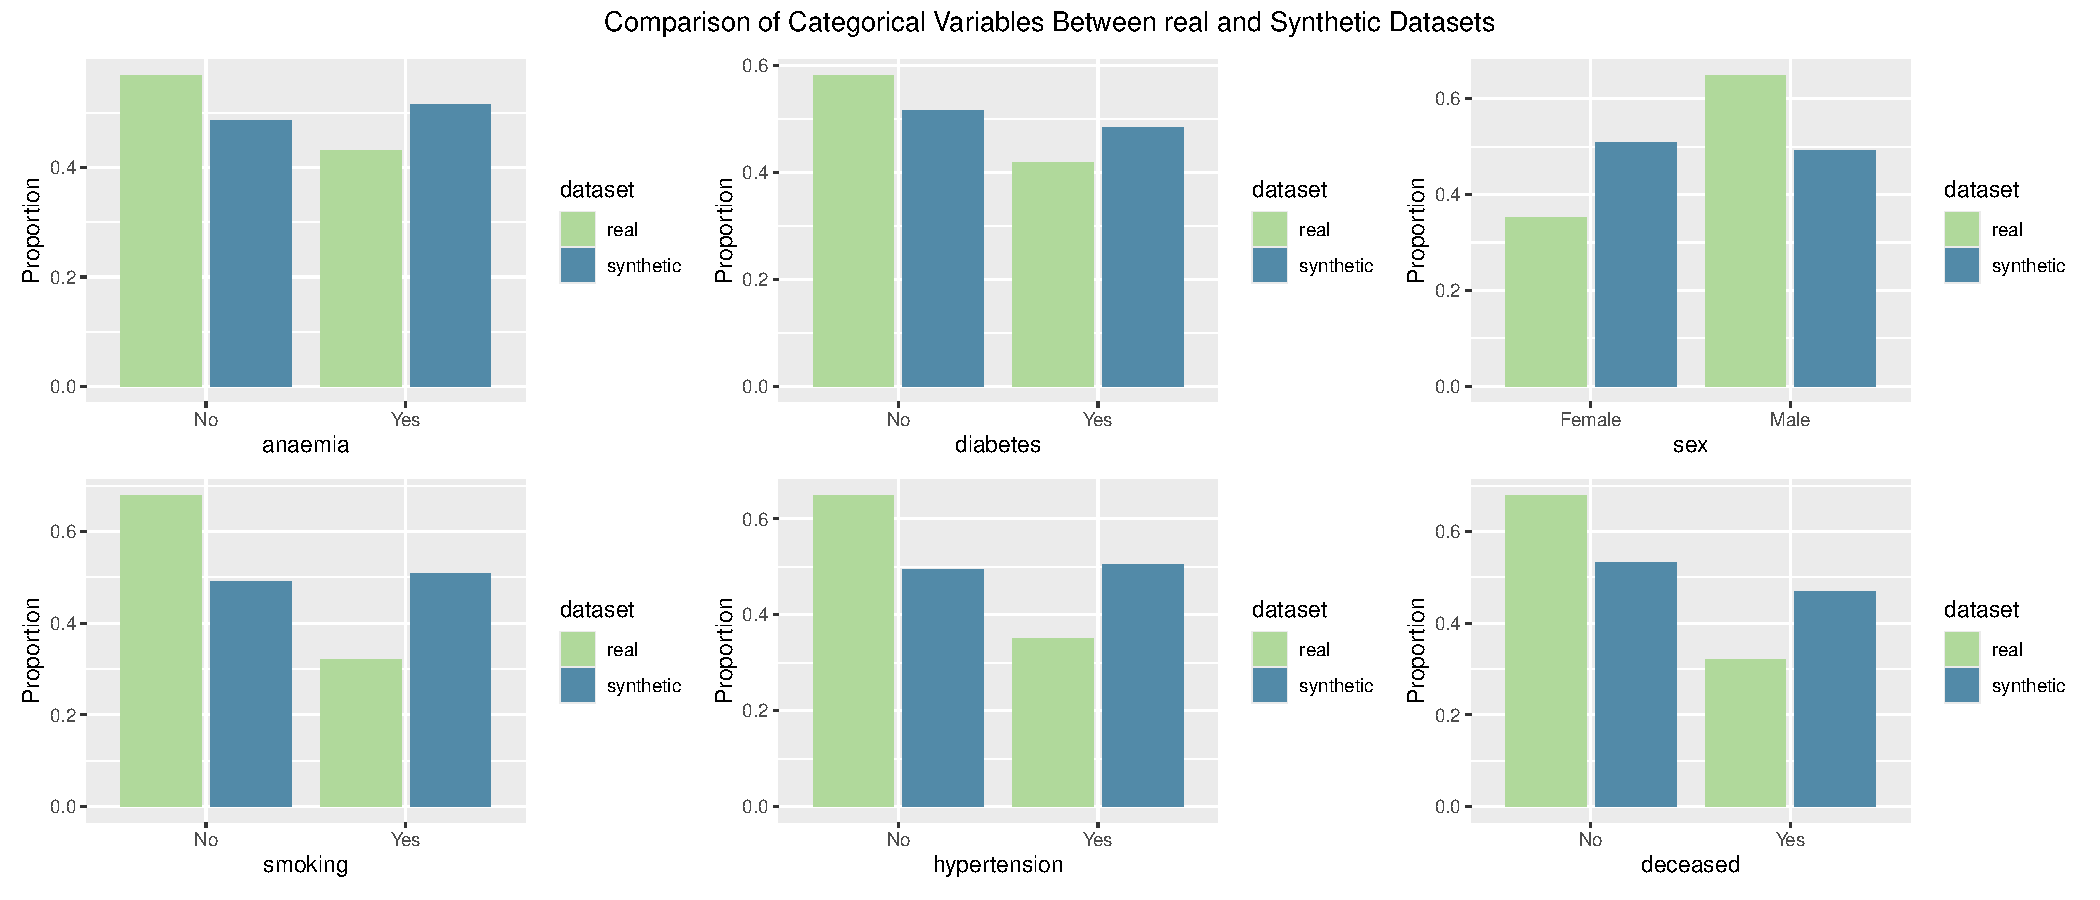
\includegraphics[width=1\linewidth,height=\textheight,keepaspectratio]{heart_failure_synthetic_data_project_files/figure-pdf/Bar plots for categorical variables (Metadata-based synthetic data)-1.pdf}
\end{center}

\subparagraph{Density Plots for Numeric
Variables}\label{density-plots-for-numeric-variables-3}

The density plots for numeric variables compare the distribution of
numeric values between the real and metadata-based synthetic datasets.

\begin{Shaded}
\begin{Highlighting}[]
\CommentTok{\# Combine real and Metadata{-}based synthetic datasets}
\NormalTok{heart\_failure}\SpecialCharTok{$}\NormalTok{dataset }\OtherTok{\textless{}{-}} \StringTok{"real"}
\NormalTok{syn\_data\_metadata}\SpecialCharTok{$}\NormalTok{dataset }\OtherTok{\textless{}{-}} \StringTok{"synthetic"}
\NormalTok{combined\_data\_metadata }\OtherTok{\textless{}{-}} \FunctionTok{bind\_rows}\NormalTok{(heart\_failure, syn\_data\_metadata)}

\CommentTok{\# Density plots for numeric variables (Metadata{-}based synthetic data)}
\NormalTok{density\_plots\_metadata }\OtherTok{\textless{}{-}} \FunctionTok{colnames}\NormalTok{(heart\_failure)[}\FunctionTok{map\_lgl}\NormalTok{(heart\_failure, is.numeric)] }\SpecialCharTok{\%\textgreater{}\%}
  \FunctionTok{map}\NormalTok{(}\SpecialCharTok{\textasciitilde{}} \FunctionTok{ggplot}\NormalTok{(combined\_data\_metadata, }\FunctionTok{aes\_string}\NormalTok{(.x, }\AttributeTok{fill =} \StringTok{\textquotesingle{}dataset\textquotesingle{}}\NormalTok{, }\AttributeTok{group =} \StringTok{\textquotesingle{}dataset\textquotesingle{}}\NormalTok{)) }\SpecialCharTok{+}
        \FunctionTok{geom\_density}\NormalTok{(}\AttributeTok{alpha =} \FloatTok{0.5}\NormalTok{) }\SpecialCharTok{+}
        \FunctionTok{scale\_fill\_manual}\NormalTok{(}\AttributeTok{values =} \FunctionTok{c}\NormalTok{(}\StringTok{"real"} \OtherTok{=} \StringTok{"\#B0D99B"}\NormalTok{, }\StringTok{"synthetic"} \OtherTok{=} \StringTok{"\#528AA8"}\NormalTok{)) }\SpecialCharTok{+}
        \FunctionTok{labs}\NormalTok{(}\AttributeTok{x =}\NormalTok{ .x, }\AttributeTok{y =} \StringTok{"Density"}\NormalTok{)) }\SpecialCharTok{\%\textgreater{}\%}
\NormalTok{  patchwork}\SpecialCharTok{::}\FunctionTok{wrap\_plots}\NormalTok{(}\AttributeTok{ncol =} \DecValTok{2}\NormalTok{) }\SpecialCharTok{+}  \CommentTok{\# Arrange plots in 2 columns}
  \FunctionTok{plot\_annotation}\NormalTok{(}\AttributeTok{title =} \StringTok{"Comparison of Numeric Variables Between real and Synthetic Data"}\NormalTok{,}
                  \AttributeTok{theme =} \FunctionTok{theme}\NormalTok{(}\AttributeTok{plot.title =} \FunctionTok{element\_text}\NormalTok{(}\AttributeTok{hjust =} \FloatTok{0.5}\NormalTok{)))}

\CommentTok{\# Print the combined density plots with one main title}
\FunctionTok{print}\NormalTok{(density\_plots\_metadata)}
\end{Highlighting}
\end{Shaded}

\begin{center}
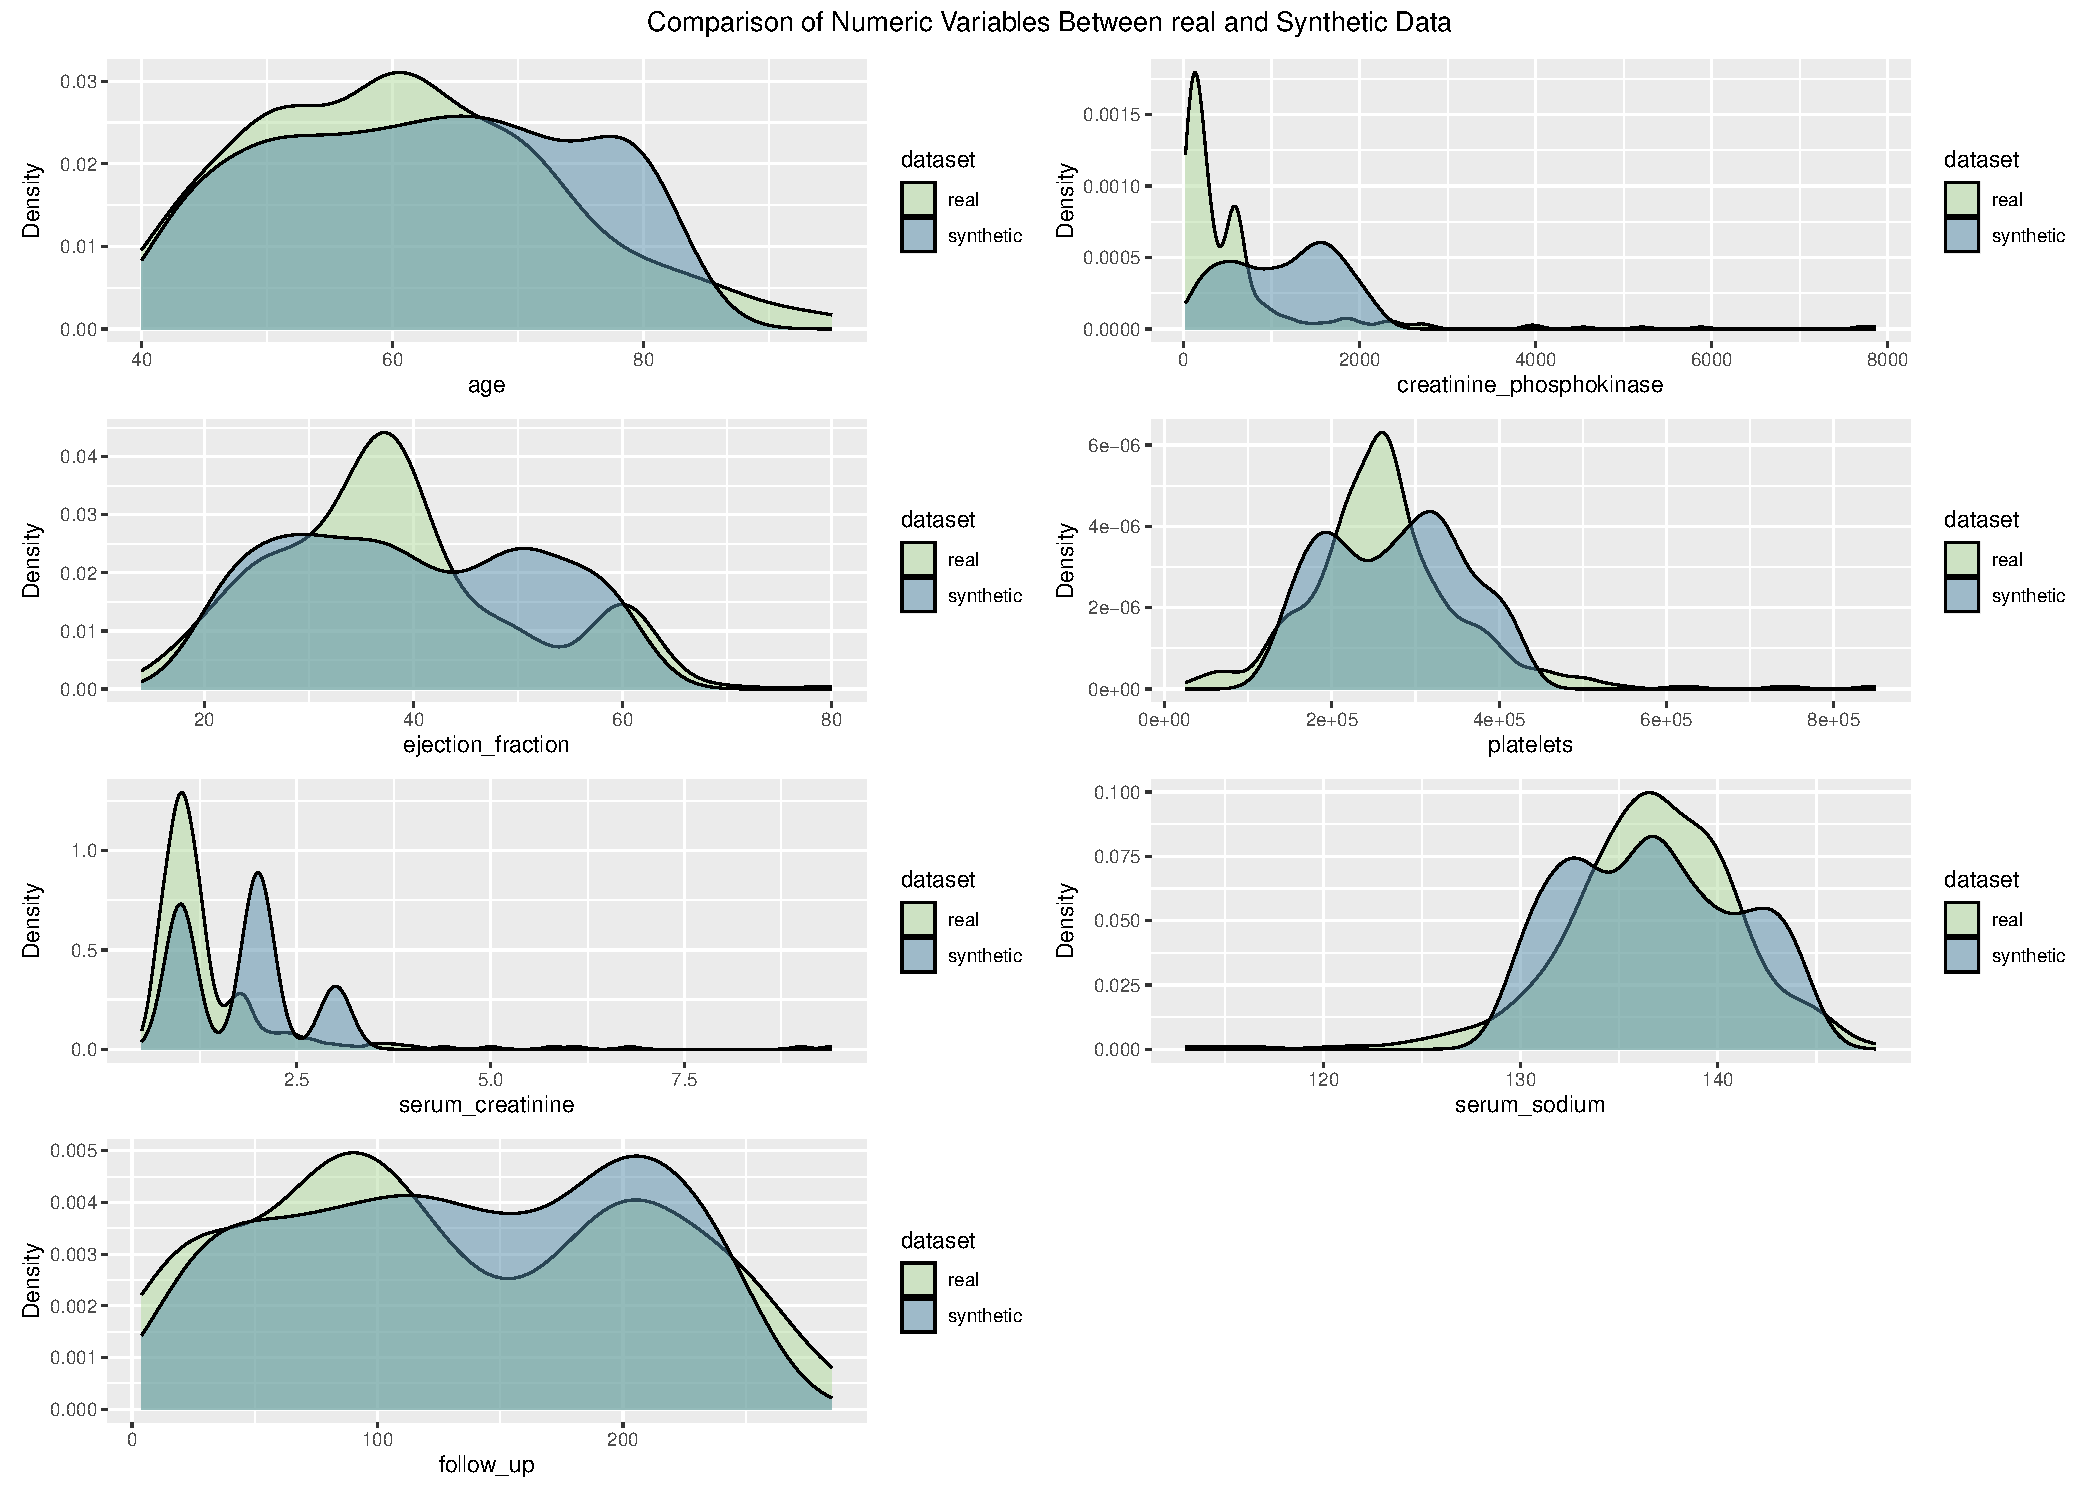
\includegraphics[width=1\linewidth,height=\textheight,keepaspectratio]{heart_failure_synthetic_data_project_files/figure-pdf/Density Plots for Numeric Variables-1.pdf}
\end{center}

\subsubsection{Histogram Similarity
Score}\label{histogram-similarity-score}

The Histogram Similarity Score measures how closely the marginal
distributions of the synthetic data match the real data. Marginal
distributions are critical for assessing whether key data
characteristics such as spread, central tendency (mean/median), and
shape (skewness/kurtosis) are preserved.

Ideal Ranges for Histogram Similarity:

\begin{itemize}
\tightlist
\item
  \textbf{Perfect Match:} 1 (100\%) indicates a perfect match between
  the distributions.
\item
  \textbf{Good Match:} 0.85--1 (85\% to 100\%) shows strong similarity.
\item
  \textbf{Moderate Match:} 0.65--0.85 suggests some differences that may
  need addressing.
\item
  \textbf{Poor Match:} Below 0.65 indicates significant deviation from
  the real data.
\end{itemize}

\begin{Shaded}
\begin{Highlighting}[]
\CommentTok{\# Custom palette for datasets}
\NormalTok{dataset\_palette }\OtherTok{\textless{}{-}} \FunctionTok{c}\NormalTok{(}
  \StringTok{"Parametric MICE"}       \OtherTok{=} \StringTok{"\#B0D99B"}\NormalTok{,}
  \StringTok{"CART Imputation"}       \OtherTok{=} \StringTok{"\#528AA8"}\NormalTok{,}
  \StringTok{"Synthpop (Low Fidelity)"} \OtherTok{=} \StringTok{"\#FFB6DB"}\NormalTok{,}
  \StringTok{"Metadata{-}Based"}        \OtherTok{=} \StringTok{"\#264653"}
\NormalTok{)}

\CommentTok{\# Define function once}
\NormalTok{calculate\_histogram\_similarity }\OtherTok{\textless{}{-}} \ControlFlowTok{function}\NormalTok{(real\_data, synthetic\_data) \{}
\NormalTok{  real\_numeric }\OtherTok{\textless{}{-}}\NormalTok{ real\_data[}\FunctionTok{sapply}\NormalTok{(real\_data, is.numeric)]}
\NormalTok{  synthetic\_numeric }\OtherTok{\textless{}{-}}\NormalTok{ synthetic\_data[}\FunctionTok{sapply}\NormalTok{(synthetic\_data, is.numeric)]}
  
\NormalTok{  similarity\_scores }\OtherTok{\textless{}{-}} \FunctionTok{sapply}\NormalTok{(}\FunctionTok{names}\NormalTok{(real\_numeric), }\ControlFlowTok{function}\NormalTok{(var) \{}
\NormalTok{    real\_hist }\OtherTok{\textless{}{-}} \FunctionTok{hist}\NormalTok{(real\_numeric[[var]], }\AttributeTok{plot =} \ConstantTok{FALSE}\NormalTok{)}
\NormalTok{    synthetic\_hist }\OtherTok{\textless{}{-}} \FunctionTok{hist}\NormalTok{(synthetic\_numeric[[var]], }\AttributeTok{plot =} \ConstantTok{FALSE}\NormalTok{)}
    
    \CommentTok{\# Wasserstein distance between histogram midpoints}
\NormalTok{    wasserstein\_distance }\OtherTok{\textless{}{-}}\NormalTok{ transport}\SpecialCharTok{::}\FunctionTok{wasserstein1d}\NormalTok{(real\_hist}\SpecialCharTok{$}\NormalTok{mids, synthetic\_hist}\SpecialCharTok{$}\NormalTok{mids)}
    \DecValTok{1} \SpecialCharTok{/}\NormalTok{ (}\DecValTok{1} \SpecialCharTok{+}\NormalTok{ wasserstein\_distance)  }\CommentTok{\# similarity score}
\NormalTok{  \})}
  
  \FunctionTok{mean}\NormalTok{(similarity\_scores)}
\NormalTok{\}}

\CommentTok{\# Collect results in a tibble (convert to percentages)}
\NormalTok{hist\_sim\_tbl }\OtherTok{\textless{}{-}}\NormalTok{ tibble}\SpecialCharTok{::}\FunctionTok{tibble}\NormalTok{(}
  \AttributeTok{Dataset =} \FunctionTok{c}\NormalTok{(}\StringTok{"Parametric MICE"}\NormalTok{, }\StringTok{"CART Imputation"}\NormalTok{, }\StringTok{"Synthpop (Low Fidelity)"}\NormalTok{, }\StringTok{"Metadata{-}Based"}\NormalTok{),}
  \AttributeTok{Histogram\_Similarity =} \FunctionTok{c}\NormalTok{(}
    \FunctionTok{calculate\_histogram\_similarity}\NormalTok{(heart\_failure, syn\_data\_1),}
    \FunctionTok{calculate\_histogram\_similarity}\NormalTok{(heart\_failure, syn\_cart\_1),}
    \FunctionTok{calculate\_histogram\_similarity}\NormalTok{(heart\_failure, syn\_data\_low\_fidelity\_synthpop),}
    \FunctionTok{calculate\_histogram\_similarity}\NormalTok{(heart\_failure, syn\_data\_metadata)}
\NormalTok{  )}
\NormalTok{) }\SpecialCharTok{\%\textgreater{}\%}
  \FunctionTok{mutate}\NormalTok{(}\AttributeTok{Histogram\_Similarity =} \FunctionTok{round}\NormalTok{(Histogram\_Similarity }\SpecialCharTok{*} \DecValTok{100}\NormalTok{, }\DecValTok{1}\NormalTok{))  }\CommentTok{\# percentage}

\CommentTok{\# Display as table}
\FunctionTok{kable}\NormalTok{(}
\NormalTok{  hist\_sim\_tbl,}
  \AttributeTok{caption =} \StringTok{"Histogram Similarity Scores (\%): higher = more similar to real data"}\NormalTok{,}
  \AttributeTok{align =} \StringTok{"lr"}
\NormalTok{)}
\end{Highlighting}
\end{Shaded}

\begin{longtable}[]{@{}lr@{}}
\caption{Histogram Similarity Scores (\%): higher = more similar to real
data}\tabularnewline
\toprule\noalign{}
Dataset & Histogram\_Similarity \\
\midrule\noalign{}
\endfirsthead
\toprule\noalign{}
Dataset & Histogram\_Similarity \\
\midrule\noalign{}
\endhead
\bottomrule\noalign{}
\endlastfoot
Parametric MICE & 9.5 \\
CART Imputation & 9.5 \\
Synthpop (Low Fidelity) & 9.5 \\
Metadata-Based & 9.5 \\
\end{longtable}

\begin{Shaded}
\begin{Highlighting}[]
\CommentTok{\# Horizontal bar chart with custom colours}
\FunctionTok{ggplot}\NormalTok{(hist\_sim\_tbl, }\FunctionTok{aes}\NormalTok{(}\AttributeTok{y =}\NormalTok{ Dataset, }\AttributeTok{x =}\NormalTok{ Histogram\_Similarity, }\AttributeTok{fill =}\NormalTok{ Dataset)) }\SpecialCharTok{+}
  \FunctionTok{geom\_col}\NormalTok{(}\AttributeTok{alpha =} \FloatTok{0.9}\NormalTok{, }\AttributeTok{show.legend =} \ConstantTok{FALSE}\NormalTok{) }\SpecialCharTok{+}
  \FunctionTok{geom\_text}\NormalTok{(}\FunctionTok{aes}\NormalTok{(}\AttributeTok{label =} \FunctionTok{paste0}\NormalTok{(Histogram\_Similarity, }\StringTok{"\%"}\NormalTok{)), }
            \AttributeTok{hjust =} \SpecialCharTok{{-}}\FloatTok{0.1}\NormalTok{, }\AttributeTok{size =} \FloatTok{3.3}\NormalTok{) }\SpecialCharTok{+}
  \FunctionTok{scale\_fill\_manual}\NormalTok{(}\AttributeTok{values =}\NormalTok{ dataset\_palette) }\SpecialCharTok{+}
  \FunctionTok{scale\_x\_continuous}\NormalTok{(}\AttributeTok{labels =}\NormalTok{ scales}\SpecialCharTok{::}\FunctionTok{percent\_format}\NormalTok{(}\AttributeTok{scale =} \DecValTok{1}\NormalTok{), }\AttributeTok{limits =} \FunctionTok{c}\NormalTok{(}\DecValTok{0}\NormalTok{, }\DecValTok{100}\NormalTok{)) }\SpecialCharTok{+}
  \FunctionTok{labs}\NormalTok{(}
    \AttributeTok{title =} \StringTok{"Histogram Similarity by Synthetic Method"}\NormalTok{,}
    \AttributeTok{subtitle =} \StringTok{"Based on Wasserstein distance of variable histograms"}\NormalTok{,}
    \AttributeTok{x =} \StringTok{"Similarity (\%)"}\NormalTok{, }\AttributeTok{y =} \ConstantTok{NULL}
\NormalTok{  ) }\SpecialCharTok{+}
  \FunctionTok{theme\_minimal}\NormalTok{() }\SpecialCharTok{+}
  \FunctionTok{theme}\NormalTok{(}\AttributeTok{axis.text.y =} \FunctionTok{element\_text}\NormalTok{(}\AttributeTok{size =} \DecValTok{10}\NormalTok{))}
\end{Highlighting}
\end{Shaded}

\begin{center}
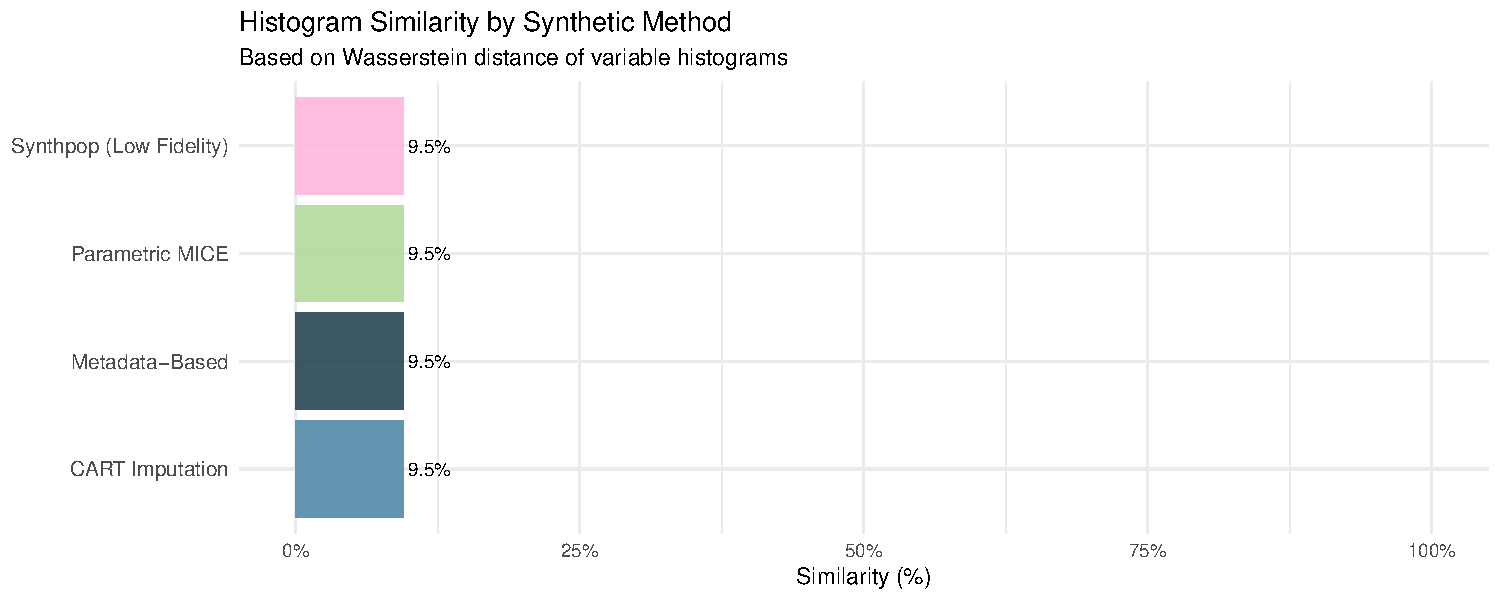
\includegraphics[width=1\linewidth,height=\textheight,keepaspectratio]{heart_failure_synthetic_data_project_files/figure-pdf/histogram-similarity-score-1.pdf}
\end{center}

\subsubsection{Mutual Information Score}\label{mutual-information-score}

The Mutual Information (MI) Score measures the shared information
between pairs of features in the real and synthetic datasets, assessing
how well relationships between variables are preserved.

Ideal Ranges for Mutual Information:

\begin{itemize}
\tightlist
\item
  \textbf{Perfect Alignment:} MI scores for synthetic data should
  ideally match the real within 10-20\% for critical feature pairs.
\item
  \textbf{Lower MI:} Consistently lower MI scores suggest that noise has
  been added, weakening relationships.
\item
  \textbf{Overfitting Risk:} Higher MI scores than the real may indicate
  overfitting, increasing re-identification risk.
\end{itemize}

\begin{Shaded}
\begin{Highlighting}[]
\CommentTok{\# Custom palette for datasets}
\NormalTok{dataset\_palette }\OtherTok{\textless{}{-}} \FunctionTok{c}\NormalTok{(}
  \StringTok{"Parametric MICE"}         \OtherTok{=} \StringTok{"\#B0D99B"}\NormalTok{,}
  \StringTok{"CART Imputation"}         \OtherTok{=} \StringTok{"\#528AA8"}\NormalTok{,}
  \StringTok{"Synthpop (Low Fidelity)"} \OtherTok{=} \StringTok{"\#FFB6DB"}\NormalTok{,}
  \StringTok{"Metadata{-}Based"}          \OtherTok{=} \StringTok{"\#264653"}
\NormalTok{)}

\CommentTok{\# {-}{-}{-}{-}{-}{-}{-} Helpers {-}{-}{-}{-}{-}{-}{-}}
\CommentTok{\# Strip \textquotesingle{}synth\_\textquotesingle{} so variable names align with the real dataset}
\NormalTok{strip\_synth\_prefix }\OtherTok{\textless{}{-}} \ControlFlowTok{function}\NormalTok{(df) \{}
  \FunctionTok{names}\NormalTok{(df) }\OtherTok{\textless{}{-}} \FunctionTok{sub}\NormalTok{(}\StringTok{"\^{}synth\_"}\NormalTok{, }\StringTok{""}\NormalTok{, }\FunctionTok{names}\NormalTok{(df))}
\NormalTok{  df}
\NormalTok{\}}

\CommentTok{\# Compute pairwise MI matrix for a data.frame of discretized columns}
\NormalTok{compute\_mi\_matrix }\OtherTok{\textless{}{-}} \ControlFlowTok{function}\NormalTok{(df\_disc) \{}
\NormalTok{  p }\OtherTok{\textless{}{-}} \FunctionTok{ncol}\NormalTok{(df\_disc)}
  \ControlFlowTok{if}\NormalTok{ (p }\SpecialCharTok{\textless{}} \DecValTok{2}\NormalTok{) }\FunctionTok{return}\NormalTok{(}\FunctionTok{matrix}\NormalTok{(}\FunctionTok{numeric}\NormalTok{(}\DecValTok{0}\NormalTok{), }\AttributeTok{nrow =}\NormalTok{ p, }\AttributeTok{ncol =}\NormalTok{ p,}
                           \AttributeTok{dimnames =} \FunctionTok{list}\NormalTok{(}\FunctionTok{colnames}\NormalTok{(df\_disc), }\FunctionTok{colnames}\NormalTok{(df\_disc))))}
\NormalTok{  M }\OtherTok{\textless{}{-}} \FunctionTok{matrix}\NormalTok{(}\DecValTok{0}\NormalTok{, }\AttributeTok{nrow =}\NormalTok{ p, }\AttributeTok{ncol =}\NormalTok{ p,}
              \AttributeTok{dimnames =} \FunctionTok{list}\NormalTok{(}\FunctionTok{colnames}\NormalTok{(df\_disc), }\FunctionTok{colnames}\NormalTok{(df\_disc)))}
  \ControlFlowTok{for}\NormalTok{ (i }\ControlFlowTok{in} \FunctionTok{seq\_len}\NormalTok{(p)) \{}
    \ControlFlowTok{for}\NormalTok{ (j }\ControlFlowTok{in}\NormalTok{ i}\SpecialCharTok{:}\NormalTok{p) \{}
      \CommentTok{\# safe MI (skip NA rows; zero if not enough variation)}
\NormalTok{      ok }\OtherTok{\textless{}{-}} \FunctionTok{is.finite}\NormalTok{(df\_disc[[i]]) }\SpecialCharTok{\&} \FunctionTok{is.finite}\NormalTok{(df\_disc[[j]])}
\NormalTok{      xi }\OtherTok{\textless{}{-}}\NormalTok{ df\_disc[[i]][ok]; xj }\OtherTok{\textless{}{-}}\NormalTok{ df\_disc[[j]][ok]}
\NormalTok{      mi }\OtherTok{\textless{}{-}} \ControlFlowTok{if}\NormalTok{ (}\FunctionTok{length}\NormalTok{(}\FunctionTok{unique}\NormalTok{(xi)) }\SpecialCharTok{\textless{}} \DecValTok{2} \SpecialCharTok{||} \FunctionTok{length}\NormalTok{(}\FunctionTok{unique}\NormalTok{(xj)) }\SpecialCharTok{\textless{}} \DecValTok{2}\NormalTok{) }\DecValTok{0} \ControlFlowTok{else}
        \FunctionTok{suppressWarnings}\NormalTok{(infotheo}\SpecialCharTok{::}\FunctionTok{mutinformation}\NormalTok{(xi, xj))}
\NormalTok{      M[i, j] }\OtherTok{\textless{}{-}}\NormalTok{ mi}
\NormalTok{      M[j, i] }\OtherTok{\textless{}{-}}\NormalTok{ mi}
\NormalTok{    \}}
\NormalTok{  \}}
\NormalTok{  M}
\NormalTok{\}}

\CommentTok{\# Compare two MI matrices (upper triangle only) {-}\textgreater{} 0–1 similarity score (higher = closer)}
\NormalTok{mi\_similarity\_score }\OtherTok{\textless{}{-}} \ControlFlowTok{function}\NormalTok{(M\_real, M\_synth) \{}
  \ControlFlowTok{if}\NormalTok{ (}\FunctionTok{length}\NormalTok{(M\_real) }\SpecialCharTok{==} \DecValTok{0} \SpecialCharTok{||} \FunctionTok{length}\NormalTok{(M\_synth) }\SpecialCharTok{==} \DecValTok{0}\NormalTok{) }\FunctionTok{return}\NormalTok{(}\ConstantTok{NA\_real\_}\NormalTok{)}
\NormalTok{  common }\OtherTok{\textless{}{-}} \FunctionTok{intersect}\NormalTok{(}\FunctionTok{colnames}\NormalTok{(M\_real), }\FunctionTok{colnames}\NormalTok{(M\_synth))}
  \ControlFlowTok{if}\NormalTok{ (}\FunctionTok{length}\NormalTok{(common) }\SpecialCharTok{\textless{}} \DecValTok{2}\NormalTok{) }\FunctionTok{return}\NormalTok{(}\ConstantTok{NA\_real\_}\NormalTok{)}
\NormalTok{  R }\OtherTok{\textless{}{-}}\NormalTok{ M\_real[common, common, drop }\OtherTok{=} \ConstantTok{FALSE}\NormalTok{]}
\NormalTok{  S }\OtherTok{\textless{}{-}}\NormalTok{ M\_synth[common, common, drop }\OtherTok{=} \ConstantTok{FALSE}\NormalTok{]}
\NormalTok{  ut }\OtherTok{\textless{}{-}} \FunctionTok{upper.tri}\NormalTok{(R, }\AttributeTok{diag =} \ConstantTok{FALSE}\NormalTok{)}
\NormalTok{  mean\_abs\_diff }\OtherTok{\textless{}{-}} \FunctionTok{mean}\NormalTok{(}\FunctionTok{abs}\NormalTok{(R[ut] }\SpecialCharTok{{-}}\NormalTok{ S[ut]))}
  \DecValTok{1} \SpecialCharTok{/}\NormalTok{ (}\DecValTok{1} \SpecialCharTok{+}\NormalTok{ mean\_abs\_diff)}
\NormalTok{\}}

\CommentTok{\# Discretize numeric columns (equal{-}frequency bins); keep only shared numeric vars}
\NormalTok{Mutual\_Information }\OtherTok{\textless{}{-}} \ControlFlowTok{function}\NormalTok{(real\_df, synth\_df, }\AttributeTok{nbins =} \DecValTok{10}\NormalTok{) \{}
\NormalTok{  real\_num  }\OtherTok{\textless{}{-}}\NormalTok{ dplyr}\SpecialCharTok{::}\FunctionTok{select}\NormalTok{(real\_df,  }\FunctionTok{where}\NormalTok{(is.numeric))}
\NormalTok{  synth\_num }\OtherTok{\textless{}{-}} \FunctionTok{strip\_synth\_prefix}\NormalTok{(synth\_df) }\SpecialCharTok{|\textgreater{}}\NormalTok{ dplyr}\SpecialCharTok{::}\FunctionTok{select}\NormalTok{(}\FunctionTok{where}\NormalTok{(is.numeric))}

\NormalTok{  common }\OtherTok{\textless{}{-}} \FunctionTok{intersect}\NormalTok{(}\FunctionTok{names}\NormalTok{(real\_num), }\FunctionTok{names}\NormalTok{(synth\_num))}
  \ControlFlowTok{if}\NormalTok{ (}\FunctionTok{length}\NormalTok{(common) }\SpecialCharTok{\textless{}} \DecValTok{2}\NormalTok{) }\FunctionTok{return}\NormalTok{(}\ConstantTok{NA\_real\_}\NormalTok{)}

\NormalTok{  real\_num  }\OtherTok{\textless{}{-}}\NormalTok{ real\_num[common]}
\NormalTok{  synth\_num }\OtherTok{\textless{}{-}}\NormalTok{ synth\_num[common]}

  \CommentTok{\# Discretize numerics (returns integer codes)}
\NormalTok{  real\_disc  }\OtherTok{\textless{}{-}} \FunctionTok{as.data.frame}\NormalTok{(}\FunctionTok{lapply}\NormalTok{(real\_num,  \textbackslash{}(x) infotheo}\SpecialCharTok{::}\FunctionTok{discretize}\NormalTok{(x, }\AttributeTok{disc =} \StringTok{"equalfreq"}\NormalTok{, }\AttributeTok{nbins =}\NormalTok{ nbins)))}
\NormalTok{  synth\_disc }\OtherTok{\textless{}{-}} \FunctionTok{as.data.frame}\NormalTok{(}\FunctionTok{lapply}\NormalTok{(synth\_num, \textbackslash{}(x) infotheo}\SpecialCharTok{::}\FunctionTok{discretize}\NormalTok{(x, }\AttributeTok{disc =} \StringTok{"equalfreq"}\NormalTok{, }\AttributeTok{nbins =}\NormalTok{ nbins)))}

  \CommentTok{\# MI matrices and similarity score}
\NormalTok{  M\_real  }\OtherTok{\textless{}{-}} \FunctionTok{compute\_mi\_matrix}\NormalTok{(real\_disc)}
\NormalTok{  M\_synth }\OtherTok{\textless{}{-}} \FunctionTok{compute\_mi\_matrix}\NormalTok{(synth\_disc)}
  \FunctionTok{mi\_similarity\_score}\NormalTok{(M\_real, M\_synth)}
\NormalTok{\}}

\CommentTok{\# {-}{-}{-}{-}{-}{-}{-} Compute scores and present nicely (percentages) {-}{-}{-}{-}{-}{-}{-}}
\NormalTok{mi\_results }\OtherTok{\textless{}{-}}\NormalTok{ tibble}\SpecialCharTok{::}\FunctionTok{tibble}\NormalTok{(}
  \AttributeTok{Dataset =} \FunctionTok{c}\NormalTok{(}\StringTok{"Parametric MICE"}\NormalTok{, }\StringTok{"CART Imputation"}\NormalTok{, }\StringTok{"Synthpop (Low Fidelity)"}\NormalTok{, }\StringTok{"Metadata{-}Based"}\NormalTok{),}
  \AttributeTok{Mutual\_Information =} \FunctionTok{c}\NormalTok{(}
    \FunctionTok{Mutual\_Information}\NormalTok{(heart\_failure, syn\_data\_1),}
    \FunctionTok{Mutual\_Information}\NormalTok{(heart\_failure, syn\_cart\_1),}
    \FunctionTok{Mutual\_Information}\NormalTok{(heart\_failure, syn\_data\_low\_fidelity\_synthpop),}
    \FunctionTok{Mutual\_Information}\NormalTok{(heart\_failure, syn\_data\_metadata)}
\NormalTok{  )}
\NormalTok{) }\SpecialCharTok{|\textgreater{}}
  \FunctionTok{mutate}\NormalTok{(}\AttributeTok{Mutual\_Information =} \FunctionTok{round}\NormalTok{(Mutual\_Information }\SpecialCharTok{*} \DecValTok{100}\NormalTok{, }\DecValTok{1}\NormalTok{))  }\CommentTok{\# convert to \%}

\CommentTok{\# User{-}friendly table}
\NormalTok{knitr}\SpecialCharTok{::}\FunctionTok{kable}\NormalTok{(}
\NormalTok{  mi\_results,}
  \AttributeTok{caption =} \StringTok{"Mutual Information Similarity (\%): higher = synthetic preserves dependency structure more closely"}\NormalTok{,}
  \AttributeTok{align =} \StringTok{"lr"}
\NormalTok{)}
\end{Highlighting}
\end{Shaded}

\begin{longtable}[]{@{}lr@{}}
\caption{Mutual Information Similarity (\%): higher = synthetic
preserves dependency structure more closely}\tabularnewline
\toprule\noalign{}
Dataset & Mutual\_Information \\
\midrule\noalign{}
\endfirsthead
\toprule\noalign{}
Dataset & Mutual\_Information \\
\midrule\noalign{}
\endhead
\bottomrule\noalign{}
\endlastfoot
Parametric MICE & 93.3 \\
CART Imputation & 94.3 \\
Synthpop (Low Fidelity) & 91.5 \\
Metadata-Based & 93.2 \\
\end{longtable}

\begin{Shaded}
\begin{Highlighting}[]
\CommentTok{\# Horizontal bar chart with custom colours}
\FunctionTok{ggplot}\NormalTok{(mi\_results, }\FunctionTok{aes}\NormalTok{(}\AttributeTok{y =}\NormalTok{ Dataset, }\AttributeTok{x =}\NormalTok{ Mutual\_Information, }\AttributeTok{fill =}\NormalTok{ Dataset)) }\SpecialCharTok{+}
  \FunctionTok{geom\_col}\NormalTok{(}\AttributeTok{alpha =} \FloatTok{0.9}\NormalTok{, }\AttributeTok{show.legend =} \ConstantTok{FALSE}\NormalTok{) }\SpecialCharTok{+}
  \FunctionTok{geom\_text}\NormalTok{(}\FunctionTok{aes}\NormalTok{(}\AttributeTok{label =} \FunctionTok{paste0}\NormalTok{(Mutual\_Information, }\StringTok{"\%"}\NormalTok{)), }
            \AttributeTok{hjust =} \SpecialCharTok{{-}}\FloatTok{0.1}\NormalTok{, }\AttributeTok{size =} \FloatTok{3.3}\NormalTok{) }\SpecialCharTok{+}
  \FunctionTok{scale\_fill\_manual}\NormalTok{(}\AttributeTok{values =}\NormalTok{ dataset\_palette) }\SpecialCharTok{+}
  \FunctionTok{scale\_x\_continuous}\NormalTok{(}\AttributeTok{labels =}\NormalTok{ scales}\SpecialCharTok{::}\FunctionTok{percent\_format}\NormalTok{(}\AttributeTok{scale =} \DecValTok{1}\NormalTok{), }\AttributeTok{limits =} \FunctionTok{c}\NormalTok{(}\DecValTok{0}\NormalTok{, }\DecValTok{100}\NormalTok{)) }\SpecialCharTok{+}
  \FunctionTok{labs}\NormalTok{(}
    \AttributeTok{title =} \StringTok{"Mutual Information Similarity by Synthetic Method"}\NormalTok{,}
    \AttributeTok{subtitle =} \StringTok{"Based on pairwise MI matrices of discretized numeric variables (equal{-}frequency bins)"}\NormalTok{,}
    \AttributeTok{x =} \StringTok{"Similarity (\%)"}\NormalTok{, }\AttributeTok{y =} \ConstantTok{NULL}
\NormalTok{  ) }\SpecialCharTok{+}
  \FunctionTok{theme\_minimal}\NormalTok{() }\SpecialCharTok{+}
  \FunctionTok{theme}\NormalTok{(}\AttributeTok{axis.text.y =} \FunctionTok{element\_text}\NormalTok{(}\AttributeTok{size =} \DecValTok{10}\NormalTok{))}
\end{Highlighting}
\end{Shaded}

\begin{center}
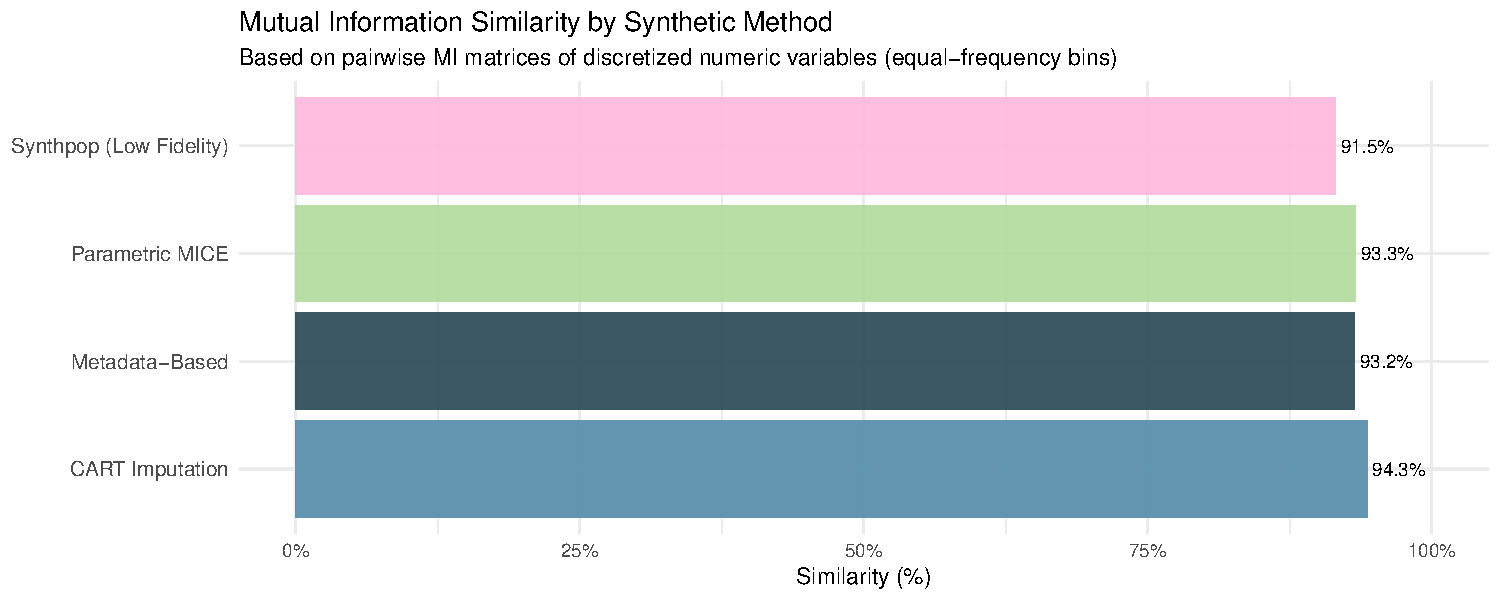
\includegraphics[width=1\linewidth,height=\textheight,keepaspectratio]{heart_failure_synthetic_data_project_files/figure-pdf/mutual-information-score-1.pdf}
\end{center}

\subsubsection{Correlation Score}\label{correlation-score}

The Correlation Score measures how well the relationships (correlations)
between variables are preserved in the synthetic dataset compared to the
real.

Ideal Ranges for Correlation Score:

\begin{itemize}
\tightlist
\item
  \textbf{Perfect Alignment:} Correlations in the synthetic data should
  match the real closely, with deviations of 5-10\% being acceptable.
\item
  \textbf{Weaker Correlations:} If synthetic correlations are weaker, it
  may indicate loss of fidelity due to noise.
\item
  \textbf{Stronger Correlations:} Stronger correlations suggest
  overfitting, which may increase privacy risks.
\end{itemize}

\begin{Shaded}
\begin{Highlighting}[]
\CommentTok{\# Custom palette for datasets}
\NormalTok{dataset\_palette }\OtherTok{\textless{}{-}} \FunctionTok{c}\NormalTok{(}
  \StringTok{"Parametric MICE"}         \OtherTok{=} \StringTok{"\#B0D99B"}\NormalTok{,}
  \StringTok{"CART Imputation"}         \OtherTok{=} \StringTok{"\#528AA8"}\NormalTok{,}
  \StringTok{"Synthpop (Low Fidelity)"} \OtherTok{=} \StringTok{"\#FFB6DB"}\NormalTok{,}
  \StringTok{"Metadata{-}Based"}          \OtherTok{=} \StringTok{"\#264653"}
\NormalTok{)}

\CommentTok{\# {-}{-}{-} Helper: strip \textquotesingle{}synth\_\textquotesingle{} so names align}
\NormalTok{strip\_synth\_prefix }\OtherTok{\textless{}{-}} \ControlFlowTok{function}\NormalTok{(df) \{}
  \FunctionTok{names}\NormalTok{(df) }\OtherTok{\textless{}{-}} \FunctionTok{sub}\NormalTok{(}\StringTok{"\^{}synth\_"}\NormalTok{, }\StringTok{""}\NormalTok{, }\FunctionTok{names}\NormalTok{(df))}
\NormalTok{  df}
\NormalTok{\}}

\CommentTok{\# {-}{-}{-} Function to calculate Correlation Similarity Score}
\NormalTok{calculate\_correlation\_score }\OtherTok{\textless{}{-}} \ControlFlowTok{function}\NormalTok{(real\_data, synthetic\_data) \{}
  \CommentTok{\# Keep numeric columns only}
\NormalTok{  real\_num  }\OtherTok{\textless{}{-}}\NormalTok{ real\_data[}\FunctionTok{sapply}\NormalTok{(real\_data, is.numeric)]}
\NormalTok{  synth\_num }\OtherTok{\textless{}{-}} \FunctionTok{strip\_synth\_prefix}\NormalTok{(synthetic\_data)[}\FunctionTok{sapply}\NormalTok{(}\FunctionTok{strip\_synth\_prefix}\NormalTok{(synthetic\_data), is.numeric)]}
  
  \CommentTok{\# Use only common variables}
\NormalTok{  common }\OtherTok{\textless{}{-}} \FunctionTok{intersect}\NormalTok{(}\FunctionTok{names}\NormalTok{(real\_num), }\FunctionTok{names}\NormalTok{(synth\_num))}
  \ControlFlowTok{if}\NormalTok{ (}\FunctionTok{length}\NormalTok{(common) }\SpecialCharTok{\textless{}} \DecValTok{2}\NormalTok{) }\FunctionTok{return}\NormalTok{(}\ConstantTok{NA\_real\_}\NormalTok{)}
  
\NormalTok{  real\_corr  }\OtherTok{\textless{}{-}} \FunctionTok{cor}\NormalTok{(real\_num[common],  }\AttributeTok{use =} \StringTok{"complete.obs"}\NormalTok{)}
\NormalTok{  synth\_corr }\OtherTok{\textless{}{-}} \FunctionTok{cor}\NormalTok{(synth\_num[common], }\AttributeTok{use =} \StringTok{"complete.obs"}\NormalTok{)}
  
  \CommentTok{\# Frobenius norm difference → similarity score in [0,1]}
\NormalTok{  corr\_diff }\OtherTok{\textless{}{-}} \FunctionTok{norm}\NormalTok{(real\_corr }\SpecialCharTok{{-}}\NormalTok{ synth\_corr, }\AttributeTok{type =} \StringTok{"F"}\NormalTok{)}
  \DecValTok{1} \SpecialCharTok{/}\NormalTok{ (}\DecValTok{1} \SpecialCharTok{+}\NormalTok{ corr\_diff)}
\NormalTok{\}}

\CommentTok{\# {-}{-}{-} Compute scores for all synthetic datasets}
\NormalTok{corr\_scores }\OtherTok{\textless{}{-}}\NormalTok{ tibble}\SpecialCharTok{::}\FunctionTok{tibble}\NormalTok{(}
  \AttributeTok{Dataset =} \FunctionTok{c}\NormalTok{(}\StringTok{"Parametric MICE"}\NormalTok{, }\StringTok{"CART Imputation"}\NormalTok{, }\StringTok{"Synthpop (Low Fidelity)"}\NormalTok{, }\StringTok{"Metadata{-}Based"}\NormalTok{),}
  \AttributeTok{Correlation\_Score =} \FunctionTok{c}\NormalTok{(}
    \FunctionTok{calculate\_correlation\_score}\NormalTok{(heart\_failure, syn\_data\_1),}
    \FunctionTok{calculate\_correlation\_score}\NormalTok{(heart\_failure, syn\_cart\_1),}
    \FunctionTok{calculate\_correlation\_score}\NormalTok{(heart\_failure, syn\_data\_low\_fidelity\_synthpop),}
    \FunctionTok{calculate\_correlation\_score}\NormalTok{(heart\_failure, syn\_data\_metadata)}
\NormalTok{  )}
\NormalTok{) }\SpecialCharTok{\%\textgreater{}\%}
  \FunctionTok{mutate}\NormalTok{(}\AttributeTok{Correlation\_Score =} \FunctionTok{round}\NormalTok{(Correlation\_Score }\SpecialCharTok{*} \DecValTok{100}\NormalTok{, }\DecValTok{1}\NormalTok{))   }\CommentTok{\# convert to \%}

\CommentTok{\# {-}{-}{-} User{-}friendly table}
\FunctionTok{kable}\NormalTok{(}
\NormalTok{  corr\_scores,}
  \AttributeTok{caption =} \StringTok{"Correlation Similarity Scores (\%): higher = synthetic preserves correlation structure more closely"}\NormalTok{,}
  \AttributeTok{align =} \StringTok{"lr"}
\NormalTok{)}
\end{Highlighting}
\end{Shaded}

\begin{longtable}[]{@{}lr@{}}
\caption{Correlation Similarity Scores (\%): higher = synthetic
preserves correlation structure more closely}\tabularnewline
\toprule\noalign{}
Dataset & Correlation\_Score \\
\midrule\noalign{}
\endfirsthead
\toprule\noalign{}
Dataset & Correlation\_Score \\
\midrule\noalign{}
\endhead
\bottomrule\noalign{}
\endlastfoot
Parametric MICE & 58.3 \\
CART Imputation & 67.2 \\
Synthpop (Low Fidelity) & 53.4 \\
Metadata-Based & 55.5 \\
\end{longtable}

\begin{Shaded}
\begin{Highlighting}[]
\CommentTok{\# {-}{-}{-} Horizontal bar chart with custom colours}
\FunctionTok{ggplot}\NormalTok{(corr\_scores, }\FunctionTok{aes}\NormalTok{(}\AttributeTok{y =}\NormalTok{ Dataset, }\AttributeTok{x =}\NormalTok{ Correlation\_Score, }\AttributeTok{fill =}\NormalTok{ Dataset)) }\SpecialCharTok{+}
  \FunctionTok{geom\_col}\NormalTok{(}\AttributeTok{alpha =} \FloatTok{0.9}\NormalTok{, }\AttributeTok{show.legend =} \ConstantTok{FALSE}\NormalTok{) }\SpecialCharTok{+}
  \FunctionTok{geom\_text}\NormalTok{(}\FunctionTok{aes}\NormalTok{(}\AttributeTok{label =} \FunctionTok{paste0}\NormalTok{(Correlation\_Score, }\StringTok{"\%"}\NormalTok{)), }
            \AttributeTok{hjust =} \SpecialCharTok{{-}}\FloatTok{0.1}\NormalTok{, }\AttributeTok{size =} \FloatTok{3.3}\NormalTok{) }\SpecialCharTok{+}
  \FunctionTok{scale\_fill\_manual}\NormalTok{(}\AttributeTok{values =}\NormalTok{ dataset\_palette) }\SpecialCharTok{+}
  \FunctionTok{scale\_x\_continuous}\NormalTok{(}\AttributeTok{labels =}\NormalTok{ scales}\SpecialCharTok{::}\FunctionTok{percent\_format}\NormalTok{(}\AttributeTok{scale =} \DecValTok{1}\NormalTok{), }\AttributeTok{limits =} \FunctionTok{c}\NormalTok{(}\DecValTok{0}\NormalTok{, }\DecValTok{100}\NormalTok{)) }\SpecialCharTok{+}
  \FunctionTok{labs}\NormalTok{(}
    \AttributeTok{title =} \StringTok{"Correlation Similarity by Synthetic Method"}\NormalTok{,}
    \AttributeTok{subtitle =} \StringTok{"Based on Frobenius norm difference between real and synthetic correlation matrices"}\NormalTok{,}
    \AttributeTok{x =} \StringTok{"Similarity (\%)"}\NormalTok{, }\AttributeTok{y =} \ConstantTok{NULL}
\NormalTok{  ) }\SpecialCharTok{+}
  \FunctionTok{theme\_minimal}\NormalTok{() }\SpecialCharTok{+}
  \FunctionTok{theme}\NormalTok{(}\AttributeTok{axis.text.y =} \FunctionTok{element\_text}\NormalTok{(}\AttributeTok{size =} \DecValTok{10}\NormalTok{))}
\end{Highlighting}
\end{Shaded}

\begin{center}
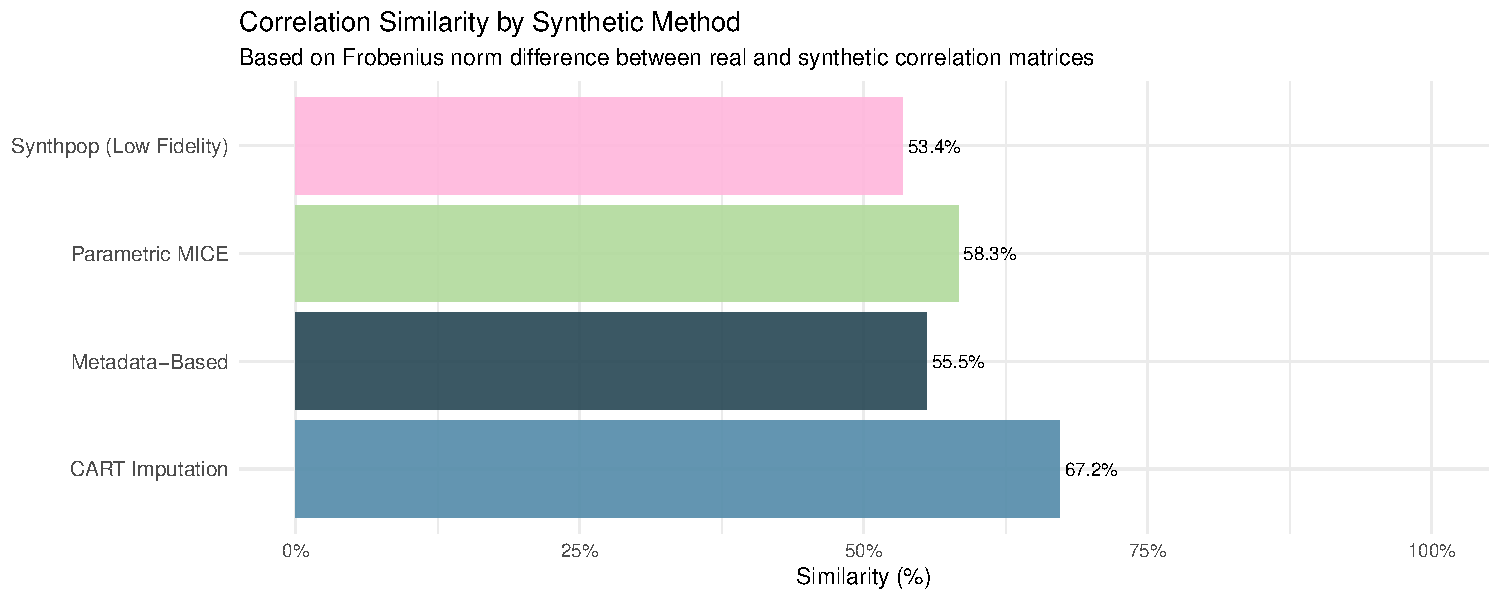
\includegraphics[width=1\linewidth,height=\textheight,keepaspectratio]{heart_failure_synthetic_data_project_files/figure-pdf/correlation-score-1.pdf}
\end{center}

\subsection{Utility Assessment}\label{utility-assessment}

\subsubsection{Feature Importance Consistency
Assessment}\label{feature-importance-consistency-assessment}

The Feature Importance Consistency Assessment evaluates how well the
synthetic datasets retain the predictive significance of features
compared to the real dataset. This assessment is essential for ensuring
that the synthetic data accurately reflects the underlying relationships
that contribute to the model's predictive performance.

Feature importance measures each variable's contribution to model
predictions. Consistency in feature importance rankings between the real
and synthetic datasets serves as a crucial indicator of data quality.
Significant discrepancies may indicate deficiencies in the synthetic
data generation process, potentially affecting the performance of models
trained on synthetic data.

Ideal Ranges for Feature Importance Consistency Assessment:

\begin{itemize}
\tightlist
\item
  \textbf{Perfect Match}: Feature importance scores in the synthetic
  dataset should closely align with those in the real dataset,
  particularly for highly predictive features.
\item
  \textbf{Acceptable Deviation}: A deviation of 10-15\% is generally
  acceptable for most features. For variables identified as highly
  influential, stricter thresholds may be needed to maintain predictive
  accuracy.
\end{itemize}

Types of Deviations

\begin{itemize}
\tightlist
\item
  \textbf{Underrepresentation}: If an important feature has lower
  importance in the synthetic dataset, it may suggest that critical
  predictive relationships are not well-preserved.
\item
  \textbf{Overrepresentation}: If a feature's importance is higher in
  the synthetic data, this could indicate noise or overfitting,
  potentially distorting the model's perception of feature
  relationships.
\end{itemize}

The following visualisation techniques will be used to compare feature
importance:

\begin{itemize}
\tightlist
\item
  \textbf{Bar Plots for Feature Importance Comparison}: Bar plots will
  compare feature importance scores between the real and synthetic
  datasets. This visual comparison can reveal significant deviations.
\item
  \textbf{SHAP Summary Plots}: SHAP (SHapley Additive exPlanations)
  summary plots provide a comprehensive view of the distribution of SHAP
  values for each feature, allowing for a direct comparison between the
  real and synthetic datasets.
\end{itemize}

\begin{Shaded}
\begin{Highlighting}[]
\CommentTok{\# Prepare the data for XGBoost}
\FunctionTok{set.seed}\NormalTok{(}\DecValTok{123}\NormalTok{)  }\CommentTok{\# For reproducibility}
\NormalTok{train\_indices }\OtherTok{\textless{}{-}} \FunctionTok{sample}\NormalTok{(}\FunctionTok{seq\_len}\NormalTok{(}\FunctionTok{nrow}\NormalTok{(heart\_failure)), }\AttributeTok{size =} \FloatTok{0.7} \SpecialCharTok{*} \FunctionTok{nrow}\NormalTok{(heart\_failure))}
\NormalTok{train\_real }\OtherTok{\textless{}{-}}\NormalTok{ heart\_failure[train\_indices, ]}
\NormalTok{test\_real }\OtherTok{\textless{}{-}}\NormalTok{ heart\_failure[}\SpecialCharTok{{-}}\NormalTok{train\_indices, ]}

\NormalTok{train\_real\_matrix }\OtherTok{\textless{}{-}} \FunctionTok{model.matrix}\NormalTok{(deceased }\SpecialCharTok{\textasciitilde{}}\NormalTok{ age }\SpecialCharTok{+}\NormalTok{ sex }\SpecialCharTok{+}\NormalTok{ anaemia }\SpecialCharTok{+}\NormalTok{ creatinine\_phosphokinase }\SpecialCharTok{+}\NormalTok{ diabetes }\SpecialCharTok{+}\NormalTok{ ejection\_fraction }\SpecialCharTok{+}\NormalTok{ platelets }\SpecialCharTok{+}\NormalTok{ serum\_creatinine }\SpecialCharTok{+}\NormalTok{ serum\_sodium }\SpecialCharTok{+}\NormalTok{ smoking }\SpecialCharTok{+}\NormalTok{ hypertension }\SpecialCharTok{+}\NormalTok{ follow\_up }\SpecialCharTok{{-}} \DecValTok{1}\NormalTok{, }\AttributeTok{data =}\NormalTok{ train\_real)}
\NormalTok{train\_real\_label }\OtherTok{\textless{}{-}}\NormalTok{ train\_real[}\FunctionTok{rownames}\NormalTok{(train\_real\_matrix), }\StringTok{"deceased"}\NormalTok{]}
\NormalTok{train\_real\_label }\OtherTok{\textless{}{-}} \FunctionTok{as.numeric}\NormalTok{(train\_real\_label) }\SpecialCharTok{{-}} \DecValTok{1}  \CommentTok{\# Convert factor to 0 and 1}

\NormalTok{train\_synth }\OtherTok{\textless{}{-}}\NormalTok{ syn\_data\_1[train\_indices, ]}
\NormalTok{train\_synth\_matrix }\OtherTok{\textless{}{-}} \FunctionTok{model.matrix}\NormalTok{(deceased }\SpecialCharTok{\textasciitilde{}}\NormalTok{ age }\SpecialCharTok{+}\NormalTok{ sex }\SpecialCharTok{+}\NormalTok{ anaemia }\SpecialCharTok{+}\NormalTok{ creatinine\_phosphokinase }\SpecialCharTok{+}\NormalTok{ diabetes }\SpecialCharTok{+}\NormalTok{ ejection\_fraction }\SpecialCharTok{+}\NormalTok{ platelets }\SpecialCharTok{+}\NormalTok{ serum\_creatinine }\SpecialCharTok{+}\NormalTok{ serum\_sodium }\SpecialCharTok{+}\NormalTok{ smoking }\SpecialCharTok{+}\NormalTok{ hypertension }\SpecialCharTok{+}\NormalTok{ follow\_up }\SpecialCharTok{{-}} \DecValTok{1}\NormalTok{, }\AttributeTok{data =}\NormalTok{ train\_synth)}
\NormalTok{train\_synth\_label }\OtherTok{\textless{}{-}}\NormalTok{ train\_synth[}\FunctionTok{rownames}\NormalTok{(train\_synth\_matrix), }\StringTok{"deceased"}\NormalTok{]}
\NormalTok{train\_synth\_label }\OtherTok{\textless{}{-}} \FunctionTok{as.numeric}\NormalTok{(train\_synth\_label) }\SpecialCharTok{{-}} \DecValTok{1}  \CommentTok{\# Convert factor to 0 and 1}

\CommentTok{\# Convert to DMatrix format, which is required for XGBoost}
\NormalTok{dtrain\_real }\OtherTok{\textless{}{-}} \FunctionTok{xgb.DMatrix}\NormalTok{(}\AttributeTok{data =}\NormalTok{ train\_real\_matrix, }\AttributeTok{label =}\NormalTok{ train\_real\_label)}
\NormalTok{dtrain\_synth }\OtherTok{\textless{}{-}} \FunctionTok{xgb.DMatrix}\NormalTok{(}\AttributeTok{data =}\NormalTok{ train\_synth\_matrix, }\AttributeTok{label =}\NormalTok{ train\_synth\_label)}

\CommentTok{\# Set up parameters for XGBoost}
\NormalTok{params }\OtherTok{\textless{}{-}} \FunctionTok{list}\NormalTok{(}
  \AttributeTok{objective =} \StringTok{"binary:logistic"}\NormalTok{,}
  \AttributeTok{eval\_metric =} \StringTok{"auc"}\NormalTok{,  }\CommentTok{\# Use AUC as an evaluation metric}
  \AttributeTok{max\_depth =} \DecValTok{3}\NormalTok{,}
  \AttributeTok{eta =} \FloatTok{0.1}
\NormalTok{)}

\CommentTok{\# Tune hyperparameters using cross{-}validation (with parallel processing)}
\NormalTok{cv\_real }\OtherTok{\textless{}{-}} \FunctionTok{xgb.cv}\NormalTok{(}
  \AttributeTok{params =}\NormalTok{ params,}
  \AttributeTok{data =}\NormalTok{ dtrain\_real,}
  \AttributeTok{nrounds =} \DecValTok{100}\NormalTok{,}
  \AttributeTok{nfold =} \DecValTok{5}\NormalTok{,}
  \AttributeTok{verbose =} \DecValTok{0}\NormalTok{,}
  \AttributeTok{early\_stopping\_rounds =} \DecValTok{10}\NormalTok{,}
  \AttributeTok{nthread =}\NormalTok{ num\_cores  }\CommentTok{\# Number of threads for parallel processing}
\NormalTok{)}

\NormalTok{best\_nrounds\_real }\OtherTok{\textless{}{-}}\NormalTok{ cv\_real}\SpecialCharTok{$}\NormalTok{best\_iteration}

\NormalTok{cv\_synth }\OtherTok{\textless{}{-}} \FunctionTok{xgb.cv}\NormalTok{(}
  \AttributeTok{params =}\NormalTok{ params,}
  \AttributeTok{data =}\NormalTok{ dtrain\_synth,}
  \AttributeTok{nrounds =} \DecValTok{100}\NormalTok{,}
  \AttributeTok{nfold =} \DecValTok{5}\NormalTok{,}
  \AttributeTok{verbose =} \DecValTok{0}\NormalTok{,}
  \AttributeTok{early\_stopping\_rounds =} \DecValTok{10}\NormalTok{,}
  \AttributeTok{nthread =}\NormalTok{ num\_cores  }\CommentTok{\# Number of threads for parallel processing}
\NormalTok{)}

\NormalTok{best\_nrounds\_synth }\OtherTok{\textless{}{-}}\NormalTok{ cv\_synth}\SpecialCharTok{$}\NormalTok{best\_iteration}

\CommentTok{\# Train XGBoost on real data (TRTR)}
\NormalTok{xgb\_model\_trtr }\OtherTok{\textless{}{-}} \FunctionTok{xgboost}\NormalTok{(}\AttributeTok{params =}\NormalTok{ params, }\AttributeTok{data =}\NormalTok{ dtrain\_real, }\AttributeTok{nrounds =}\NormalTok{ best\_nrounds\_real, }\AttributeTok{verbose =} \DecValTok{0}\NormalTok{, }\AttributeTok{nthread =}\NormalTok{ num\_cores)}

\CommentTok{\# Train XGBoost on synthetic data (TSTR)}
\NormalTok{xgb\_model\_tstr }\OtherTok{\textless{}{-}} \FunctionTok{xgboost}\NormalTok{(}\AttributeTok{params =}\NormalTok{ params, }\AttributeTok{data =}\NormalTok{ dtrain\_synth, }\AttributeTok{nrounds =}\NormalTok{ best\_nrounds\_synth, }\AttributeTok{verbose =} \DecValTok{0}\NormalTok{, }\AttributeTok{nthread =}\NormalTok{ num\_cores)}

\CommentTok{\# Get feature importance for TRTR}
\NormalTok{importance\_trtr }\OtherTok{\textless{}{-}} \FunctionTok{xgb.importance}\NormalTok{(}\AttributeTok{feature\_names =} \FunctionTok{colnames}\NormalTok{(train\_real\_matrix), }\AttributeTok{model =}\NormalTok{ xgb\_model\_trtr)}
\FunctionTok{cat}\NormalTok{(}\StringTok{"Feature Importance for TRTR:}\SpecialCharTok{\textbackslash{}n}\StringTok{"}\NormalTok{)}
\end{Highlighting}
\end{Shaded}

\begin{verbatim}
Feature Importance for TRTR:
\end{verbatim}

\begin{Shaded}
\begin{Highlighting}[]
\FunctionTok{print}\NormalTok{(importance\_trtr)}
\end{Highlighting}
\end{Shaded}

\begin{verbatim}
                    Feature        Gain      Cover  Frequency
                     <char>       <num>      <num>      <num>
1:                follow_up 0.550035467 0.35582680 0.26470588
2:         serum_creatinine 0.179450673 0.25780255 0.22794118
3:        ejection_fraction 0.107840968 0.17061583 0.12500000
4: creatinine_phosphokinase 0.100830923 0.12847956 0.20588235
5:             serum_sodium 0.032740748 0.04233723 0.08823529
6:                      age 0.022510598 0.03446459 0.04411765
7:                platelets 0.006590623 0.01047345 0.04411765
\end{verbatim}

\begin{Shaded}
\begin{Highlighting}[]
\CommentTok{\# Get feature importance for TSTR}
\NormalTok{importance\_tstr }\OtherTok{\textless{}{-}} \FunctionTok{xgb.importance}\NormalTok{(}\AttributeTok{feature\_names =} \FunctionTok{colnames}\NormalTok{(train\_synth\_matrix), }\AttributeTok{model =}\NormalTok{ xgb\_model\_tstr)}
\FunctionTok{cat}\NormalTok{(}\StringTok{"}\SpecialCharTok{\textbackslash{}n}\StringTok{Feature Importance for TSTR:}\SpecialCharTok{\textbackslash{}n}\StringTok{"}\NormalTok{)}
\end{Highlighting}
\end{Shaded}

\begin{verbatim}

Feature Importance for TSTR:
\end{verbatim}

\begin{Shaded}
\begin{Highlighting}[]
\FunctionTok{print}\NormalTok{(importance\_tstr)}
\end{Highlighting}
\end{Shaded}

\begin{verbatim}
                    Feature       Gain      Cover Frequency
                     <char>      <num>      <num>     <num>
1:                follow_up 0.37991328 0.37325270      0.20
2:        ejection_fraction 0.22999025 0.21347069      0.32
3:             serum_sodium 0.20146359 0.17350782      0.16
4:                platelets 0.13419963 0.10862788      0.12
5:         serum_creatinine 0.04007483 0.12057396      0.16
6: creatinine_phosphokinase 0.01435841 0.01056696      0.04
\end{verbatim}

\begin{Shaded}
\begin{Highlighting}[]
\CommentTok{\# Visualise feature importance for TRTR and TSTR}
\NormalTok{importance\_trtr}\SpecialCharTok{$}\NormalTok{Dataset }\OtherTok{\textless{}{-}} \StringTok{"Real Data"}
\NormalTok{importance\_tstr}\SpecialCharTok{$}\NormalTok{Dataset }\OtherTok{\textless{}{-}} \StringTok{"Synthetic Data"}

\NormalTok{importance\_combined }\OtherTok{\textless{}{-}} \FunctionTok{rbind}\NormalTok{(importance\_trtr, importance\_tstr)}

\CommentTok{\# Plot feature importance comparison}
\FunctionTok{ggplot}\NormalTok{(importance\_combined, }\FunctionTok{aes}\NormalTok{(}\AttributeTok{x =} \FunctionTok{reorder}\NormalTok{(Feature, Gain), }\AttributeTok{y =}\NormalTok{ Gain, }\AttributeTok{fill =}\NormalTok{ Dataset)) }\SpecialCharTok{+}
  \FunctionTok{geom\_bar}\NormalTok{(}\AttributeTok{stat =} \StringTok{"identity"}\NormalTok{, }\AttributeTok{position =} \StringTok{"dodge"}\NormalTok{) }\SpecialCharTok{+}
  \FunctionTok{coord\_flip}\NormalTok{() }\SpecialCharTok{+}
  \FunctionTok{labs}\NormalTok{(}\AttributeTok{title =} \StringTok{"Feature Importance Comparison (TRTR vs TSTR)"}\NormalTok{,}
       \AttributeTok{x =} \StringTok{"Feature"}\NormalTok{,}
       \AttributeTok{y =} \StringTok{"Gain"}\NormalTok{) }\SpecialCharTok{+}
  \FunctionTok{scale\_fill\_manual}\NormalTok{(}\AttributeTok{values =} \FunctionTok{c}\NormalTok{(}\StringTok{"Real Data"} \OtherTok{=} \StringTok{"\#B0D99B"}\NormalTok{, }\StringTok{"Synthetic Data"} \OtherTok{=} \StringTok{"\#528AA8"}\NormalTok{)) }\SpecialCharTok{+}
  \FunctionTok{theme\_minimal}\NormalTok{()}
\end{Highlighting}
\end{Shaded}

\begin{center}
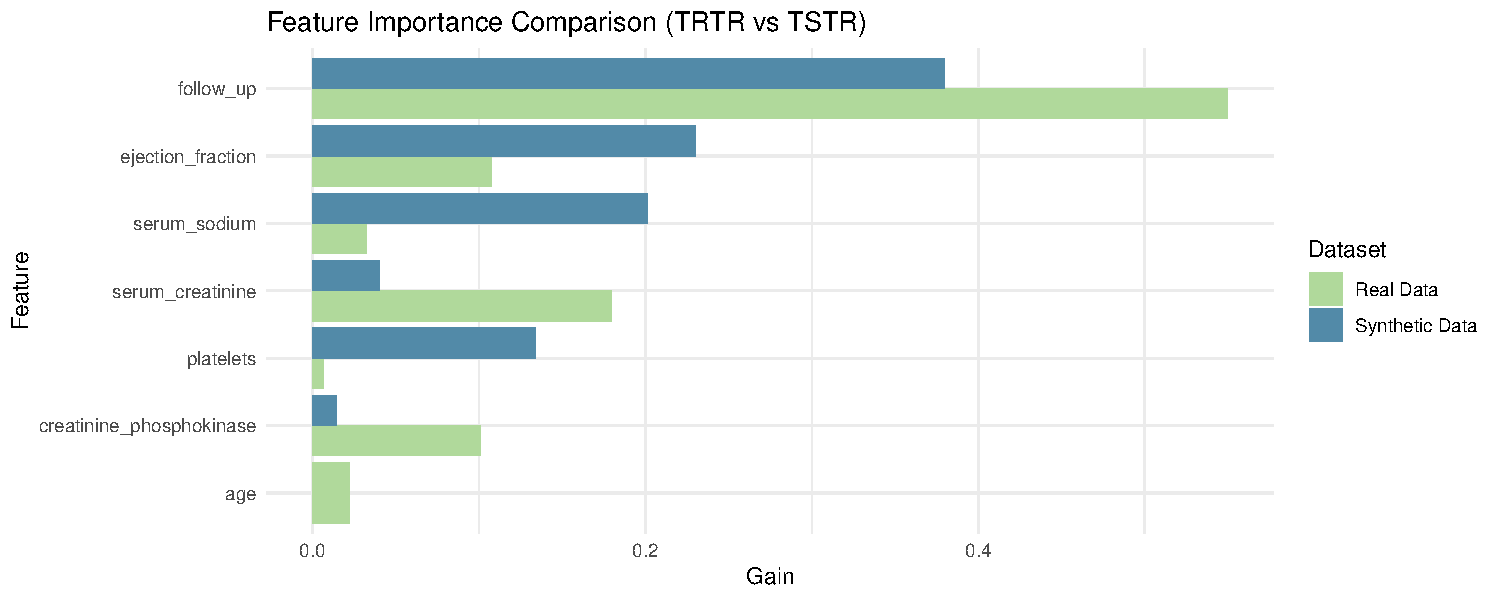
\includegraphics[width=1\linewidth,height=\textheight,keepaspectratio]{heart_failure_synthetic_data_project_files/figure-pdf/Feature Importance Consistency Assessment-1.pdf}
\end{center}

\begin{Shaded}
\begin{Highlighting}[]
\CommentTok{\# Correlation analysis between feature importance rankings}

\NormalTok{importance\_trtr }\OtherTok{\textless{}{-}}\NormalTok{ importance\_trtr }\SpecialCharTok{\%\textgreater{}\%} \FunctionTok{mutate}\NormalTok{(}\AttributeTok{rank =} \FunctionTok{rank}\NormalTok{(}\SpecialCharTok{{-}}\NormalTok{Gain))}
\NormalTok{importance\_tstr }\OtherTok{\textless{}{-}}\NormalTok{ importance\_tstr }\SpecialCharTok{\%\textgreater{}\%} \FunctionTok{mutate}\NormalTok{(}\AttributeTok{rank =} \FunctionTok{rank}\NormalTok{(}\SpecialCharTok{{-}}\NormalTok{Gain))}

\NormalTok{importance\_ranking }\OtherTok{\textless{}{-}} \FunctionTok{inner\_join}\NormalTok{(importance\_trtr, importance\_tstr, }\AttributeTok{by =} \StringTok{"Feature"}\NormalTok{, }\AttributeTok{suffix =} \FunctionTok{c}\NormalTok{(}\StringTok{"\_trtr"}\NormalTok{, }\StringTok{"\_tstr"}\NormalTok{))}

\NormalTok{correlation }\OtherTok{\textless{}{-}} \FunctionTok{cor}\NormalTok{(importance\_ranking}\SpecialCharTok{$}\NormalTok{rank\_trtr, importance\_ranking}\SpecialCharTok{$}\NormalTok{rank\_tstr, }\AttributeTok{method =} \StringTok{"spearman"}\NormalTok{)}
\FunctionTok{cat}\NormalTok{(}\StringTok{"}\SpecialCharTok{\textbackslash{}n}\StringTok{Spearman correlation Between TRTR and TSTR Feature Importance Rankings:}\SpecialCharTok{\textbackslash{}n}\StringTok{"}\NormalTok{)}
\end{Highlighting}
\end{Shaded}

\begin{verbatim}

Spearman correlation Between TRTR and TSTR Feature Importance Rankings:
\end{verbatim}

\begin{Shaded}
\begin{Highlighting}[]
\FunctionTok{print}\NormalTok{(correlation)}
\end{Highlighting}
\end{Shaded}

\begin{verbatim}
[1] 0.3714286
\end{verbatim}

\begin{Shaded}
\begin{Highlighting}[]
\CommentTok{\# Calculate SHAP values for better interpretability}

\CommentTok{\# SHAP values for TRTR}
\NormalTok{shap\_values\_trtr }\OtherTok{\textless{}{-}} \FunctionTok{shap.values}\NormalTok{(xgb\_model\_trtr, dtrain\_real)}
\NormalTok{shap\_long\_trtr }\OtherTok{\textless{}{-}} \FunctionTok{shap.prep}\NormalTok{(}\AttributeTok{shap\_contrib =}\NormalTok{ shap\_values\_trtr}\SpecialCharTok{$}\NormalTok{shap\_score, }\AttributeTok{X\_train =}\NormalTok{ train\_real\_matrix)}

\FunctionTok{cat}\NormalTok{(}\StringTok{"}\SpecialCharTok{\textbackslash{}n}\StringTok{SHAP Summary for TRTR:}\SpecialCharTok{\textbackslash{}n}\StringTok{"}\NormalTok{)}
\end{Highlighting}
\end{Shaded}

\begin{verbatim}

SHAP Summary for TRTR:
\end{verbatim}

\begin{Shaded}
\begin{Highlighting}[]
\NormalTok{shap\_values\_trtr}\SpecialCharTok{$}\NormalTok{mean\_shap\_score }\SpecialCharTok{\%\textgreater{}\%} \FunctionTok{print}\NormalTok{()}
\end{Highlighting}
\end{Shaded}

\begin{verbatim}
               follow_up         serum_creatinine        ejection_fraction 
              0.92293409               0.52780225               0.39932806 
creatinine_phosphokinase             serum_sodium                      age 
              0.18850937               0.10067811               0.06711965 
               platelets                sexFemale                  sexMale 
              0.02991459               0.00000000               0.00000000 
              anaemiaYes              diabetesYes               smokingYes 
              0.00000000               0.00000000               0.00000000 
         hypertensionYes 
              0.00000000 
\end{verbatim}

\begin{Shaded}
\begin{Highlighting}[]
\CommentTok{\# SHAP values for TSTR}
\NormalTok{shap\_values\_tstr }\OtherTok{\textless{}{-}} \FunctionTok{shap.values}\NormalTok{(xgb\_model\_tstr, dtrain\_synth)}
\NormalTok{shap\_long\_tstr }\OtherTok{\textless{}{-}} \FunctionTok{shap.prep}\NormalTok{(}\AttributeTok{shap\_contrib =}\NormalTok{ shap\_values\_tstr}\SpecialCharTok{$}\NormalTok{shap\_score, }\AttributeTok{X\_train =}\NormalTok{ train\_synth\_matrix)}

\FunctionTok{cat}\NormalTok{(}\StringTok{"}\SpecialCharTok{\textbackslash{}n}\StringTok{SHAP Summary for TSTR:}\SpecialCharTok{\textbackslash{}n}\StringTok{"}\NormalTok{)}
\end{Highlighting}
\end{Shaded}

\begin{verbatim}

SHAP Summary for TSTR:
\end{verbatim}

\begin{Shaded}
\begin{Highlighting}[]
\NormalTok{shap\_values\_tstr}\SpecialCharTok{$}\NormalTok{mean\_shap\_score }\SpecialCharTok{\%\textgreater{}\%} \FunctionTok{print}\NormalTok{()}
\end{Highlighting}
\end{Shaded}

\begin{verbatim}
               follow_up        ejection_fraction                platelets 
             0.210816300              0.069274587              0.067060756 
            serum_sodium         serum_creatinine creatinine_phosphokinase 
             0.058853411              0.035087248              0.006947092 
                     age                sexFemale                  sexMale 
             0.000000000              0.000000000              0.000000000 
              anaemiaYes              diabetesYes               smokingYes 
             0.000000000              0.000000000              0.000000000 
         hypertensionYes 
             0.000000000 
\end{verbatim}

\begin{Shaded}
\begin{Highlighting}[]
\CommentTok{\# SHAP visualisation}
\FunctionTok{shap.plot.summary}\NormalTok{(shap\_long\_trtr)}
\end{Highlighting}
\end{Shaded}

\begin{center}
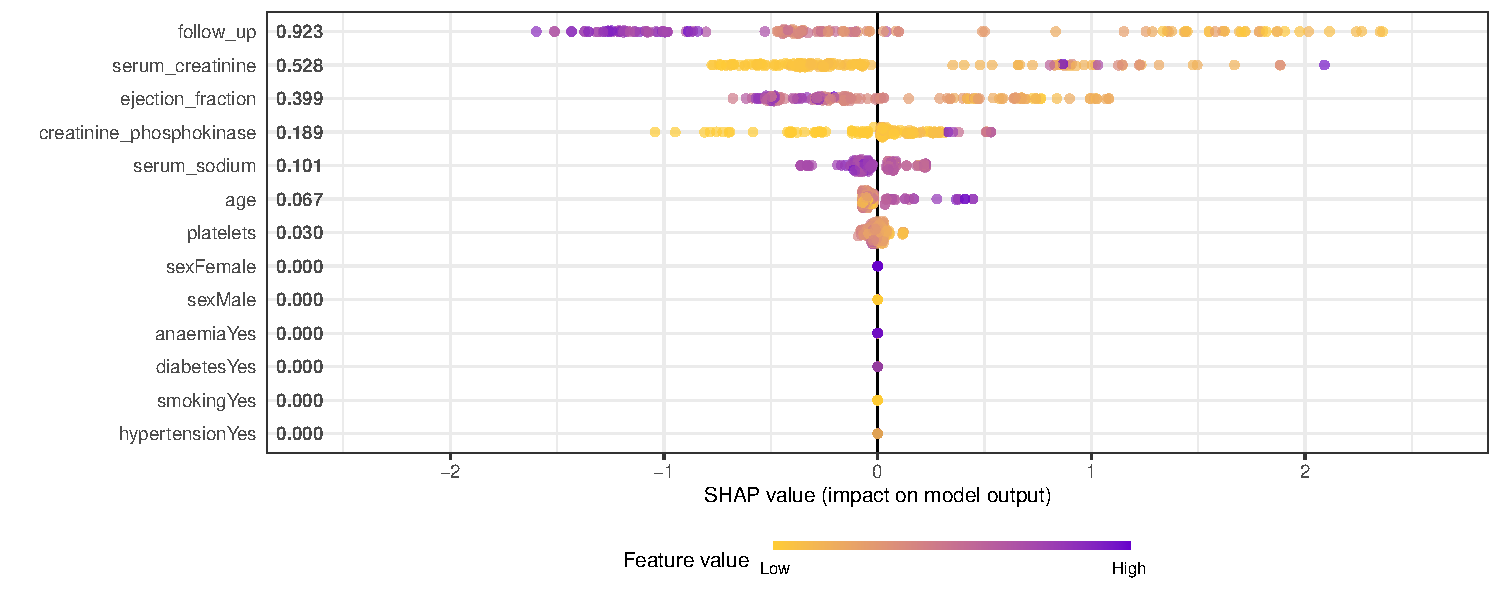
\includegraphics[width=1\linewidth,height=\textheight,keepaspectratio]{heart_failure_synthetic_data_project_files/figure-pdf/Feature Importance Consistency Assessment-2.pdf}
\end{center}

\begin{Shaded}
\begin{Highlighting}[]
\FunctionTok{shap.plot.summary}\NormalTok{(shap\_long\_tstr)}
\end{Highlighting}
\end{Shaded}

\begin{center}
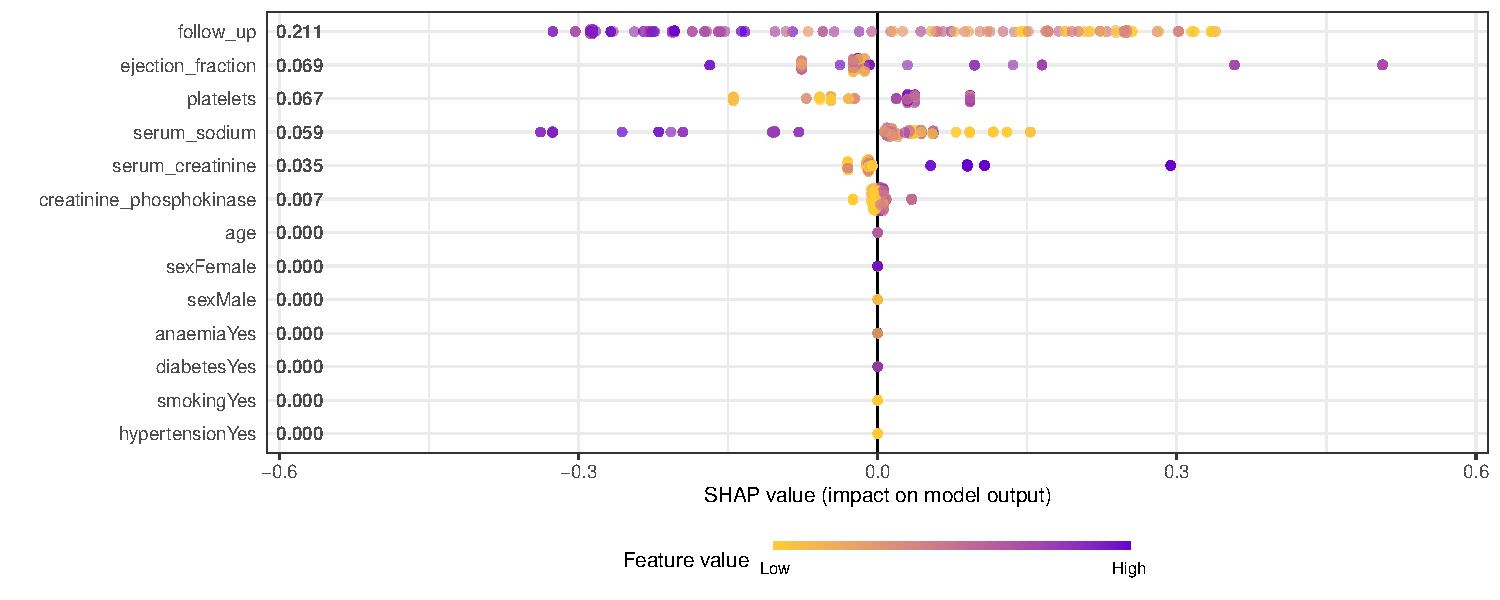
\includegraphics[width=1\linewidth,height=\textheight,keepaspectratio]{heart_failure_synthetic_data_project_files/figure-pdf/Feature Importance Consistency Assessment-3.pdf}
\end{center}

\subsubsection{Prediction Score}\label{prediction-score}

The Prediction Score assesses synthetic data utility by comparing models
trained on real data (Train Real Test Real (TRTR)) versus synthetic data
(Train Synthetic Test Real (TSTR)) using two metrics:

\begin{itemize}
\tightlist
\item
  \textbf{Accuracy}: The proportion of correct predictions made by the
  model.
\item
  \textbf{pMSE (Prediction Mean Squared Error)}: Measures the average of
  the squared differences between predicted and actual values.
\end{itemize}

Ideal Ranges for Prediction Score:

\begin{itemize}
\tightlist
\item
  \textbf{Accuracy}: TSTR accuracy should be within 5-10\% of TRTR
  accuracy. Lower accuracy signals that synthetic data isn't fully
  representative of the real dataset.
\item
  \textbf{pMSE}: TSTR pMSE should be close to TRTR pMSE. A 5-10\%
  deviation is acceptable; a higher pMSE suggests synthetic data may not
  be accurately reflecting the true relationships in the real data.
\end{itemize}

This section assesses the utility of synthetic data generated through
various methods, using XGBoost to calculate both Accuracy and pMSE for
TRTR and TSTR.

\begin{Shaded}
\begin{Highlighting}[]
\FunctionTok{set.seed}\NormalTok{(}\DecValTok{123}\NormalTok{)}

\CommentTok{\# {-}{-}{-}{-} helpers {-}{-}{-}{-}}
\NormalTok{strip\_synth\_prefix }\OtherTok{\textless{}{-}} \ControlFlowTok{function}\NormalTok{(df) \{ }\FunctionTok{names}\NormalTok{(df) }\OtherTok{\textless{}{-}} \FunctionTok{sub}\NormalTok{(}\StringTok{"\^{}synth\_"}\NormalTok{, }\StringTok{""}\NormalTok{, }\FunctionTok{names}\NormalTok{(df)); df \}}

\NormalTok{align\_target\_levels }\OtherTok{\textless{}{-}} \ControlFlowTok{function}\NormalTok{(df, }\AttributeTok{levels\_ref =} \ConstantTok{NULL}\NormalTok{, }\AttributeTok{positive =} \ConstantTok{NULL}\NormalTok{) \{}
  \ControlFlowTok{if}\NormalTok{ (}\SpecialCharTok{!}\FunctionTok{is.factor}\NormalTok{(df}\SpecialCharTok{$}\NormalTok{deceased)) \{}
    \ControlFlowTok{if}\NormalTok{ (}\FunctionTok{is.numeric}\NormalTok{(df}\SpecialCharTok{$}\NormalTok{deceased)) df}\SpecialCharTok{$}\NormalTok{deceased }\OtherTok{\textless{}{-}} \FunctionTok{factor}\NormalTok{(}\FunctionTok{as.character}\NormalTok{(df}\SpecialCharTok{$}\NormalTok{deceased)) }\ControlFlowTok{else}\NormalTok{ df}\SpecialCharTok{$}\NormalTok{deceased }\OtherTok{\textless{}{-}} \FunctionTok{factor}\NormalTok{(df}\SpecialCharTok{$}\NormalTok{deceased)}
\NormalTok{  \}}
  \ControlFlowTok{if}\NormalTok{ (}\SpecialCharTok{!}\FunctionTok{is.null}\NormalTok{(levels\_ref)) df}\SpecialCharTok{$}\NormalTok{deceased }\OtherTok{\textless{}{-}} \FunctionTok{factor}\NormalTok{(df}\SpecialCharTok{$}\NormalTok{deceased, }\AttributeTok{levels =}\NormalTok{ levels\_ref)}
\NormalTok{  lev }\OtherTok{\textless{}{-}} \FunctionTok{levels}\NormalTok{(df}\SpecialCharTok{$}\NormalTok{deceased)}
  \ControlFlowTok{if}\NormalTok{ (}\FunctionTok{length}\NormalTok{(lev) }\SpecialCharTok{\textless{}} \DecValTok{2}\NormalTok{) }\FunctionTok{stop}\NormalTok{(}\StringTok{"Target \textquotesingle{}deceased\textquotesingle{} must have two levels."}\NormalTok{)}
\NormalTok{  pos }\OtherTok{\textless{}{-}} \ControlFlowTok{if}\NormalTok{ (}\SpecialCharTok{!}\FunctionTok{is.null}\NormalTok{(positive) }\SpecialCharTok{\&\&}\NormalTok{ positive }\SpecialCharTok{\%in\%}\NormalTok{ lev) positive }\ControlFlowTok{else} \ControlFlowTok{if}\NormalTok{ (}\StringTok{"1"} \SpecialCharTok{\%in\%}\NormalTok{ lev) }\StringTok{"1"} \ControlFlowTok{else}\NormalTok{ lev[}\DecValTok{2}\NormalTok{]}
\NormalTok{  df}\SpecialCharTok{$}\NormalTok{deceased }\OtherTok{\textless{}{-}}\NormalTok{ stats}\SpecialCharTok{::}\FunctionTok{relevel}\NormalTok{(df}\SpecialCharTok{$}\NormalTok{deceased, }\AttributeTok{ref =}\NormalTok{ pos)}
  \FunctionTok{list}\NormalTok{(}\AttributeTok{data =}\NormalTok{ df, }\AttributeTok{levels =} \FunctionTok{levels}\NormalTok{(df}\SpecialCharTok{$}\NormalTok{deceased), }\AttributeTok{positive =}\NormalTok{ pos)}
\NormalTok{\}}

\NormalTok{evaluate\_model }\OtherTok{\textless{}{-}} \ControlFlowTok{function}\NormalTok{(train\_data, test\_data, label, tune\_grid, train\_control, }\AttributeTok{seed =} \DecValTok{123}\NormalTok{) \{}
\NormalTok{  test\_aln  }\OtherTok{\textless{}{-}} \FunctionTok{align\_target\_levels}\NormalTok{(test\_data)}
\NormalTok{  train\_aln }\OtherTok{\textless{}{-}} \FunctionTok{align\_target\_levels}\NormalTok{(train\_data, }\AttributeTok{levels\_ref =}\NormalTok{ test\_aln}\SpecialCharTok{$}\NormalTok{levels, }\AttributeTok{positive =}\NormalTok{ test\_aln}\SpecialCharTok{$}\NormalTok{positive)}
\NormalTok{  train\_data }\OtherTok{\textless{}{-}}\NormalTok{ train\_aln}\SpecialCharTok{$}\NormalTok{data}
\NormalTok{  test\_data  }\OtherTok{\textless{}{-}}\NormalTok{ test\_aln}\SpecialCharTok{$}\NormalTok{data}

  \FunctionTok{set.seed}\NormalTok{(seed)}
\NormalTok{  model }\OtherTok{\textless{}{-}}\NormalTok{ caret}\SpecialCharTok{::}\FunctionTok{train}\NormalTok{(}
\NormalTok{    deceased }\SpecialCharTok{\textasciitilde{}}\NormalTok{ follow\_up }\SpecialCharTok{+}\NormalTok{ serum\_creatinine }\SpecialCharTok{+}\NormalTok{ ejection\_fraction }\SpecialCharTok{+}
\NormalTok{      creatinine\_phosphokinase }\SpecialCharTok{+}\NormalTok{ serum\_sodium }\SpecialCharTok{+}\NormalTok{ age }\SpecialCharTok{+}\NormalTok{ platelets,}
    \AttributeTok{data      =}\NormalTok{ train\_data,}
    \AttributeTok{method    =} \StringTok{"xgbTree"}\NormalTok{,}
    \AttributeTok{trControl =}\NormalTok{ train\_control,}
    \AttributeTok{tuneGrid  =}\NormalTok{ tune\_grid,}
    \AttributeTok{na.action =}\NormalTok{ na.pass}
\NormalTok{  )}

\NormalTok{  pred }\OtherTok{\textless{}{-}} \FunctionTok{predict}\NormalTok{(model, test\_data)}
\NormalTok{  acc  }\OtherTok{\textless{}{-}} \FunctionTok{mean}\NormalTok{(pred }\SpecialCharTok{==}\NormalTok{ test\_data}\SpecialCharTok{$}\NormalTok{deceased, }\AttributeTok{na.rm =} \ConstantTok{TRUE}\NormalTok{)}
\NormalTok{  yhat }\OtherTok{\textless{}{-}} \FunctionTok{as.numeric}\NormalTok{(pred)}
\NormalTok{  y    }\OtherTok{\textless{}{-}} \FunctionTok{as.numeric}\NormalTok{(test\_data}\SpecialCharTok{$}\NormalTok{deceased)}
\NormalTok{  pMSE }\OtherTok{\textless{}{-}} \FunctionTok{mean}\NormalTok{((yhat }\SpecialCharTok{{-}}\NormalTok{ y)}\SpecialCharTok{\^{}}\DecValTok{2}\NormalTok{, }\AttributeTok{na.rm =} \ConstantTok{TRUE}\NormalTok{)}

\NormalTok{  tibble}\SpecialCharTok{::}\FunctionTok{tibble}\NormalTok{(}\AttributeTok{Dataset =}\NormalTok{ label, }\AttributeTok{Accuracy =}\NormalTok{ acc, }\AttributeTok{pMSE =}\NormalTok{ pMSE)}
\NormalTok{\}}

\CommentTok{\# {-}{-}{-}{-} CV setup {-}{-}{-}{-}}
\NormalTok{train\_control }\OtherTok{\textless{}{-}}\NormalTok{ caret}\SpecialCharTok{::}\FunctionTok{trainControl}\NormalTok{(}\AttributeTok{method =} \StringTok{"cv"}\NormalTok{, }\AttributeTok{number =} \DecValTok{5}\NormalTok{)}
\NormalTok{tune\_grid }\OtherTok{\textless{}{-}} \FunctionTok{expand.grid}\NormalTok{(}
  \AttributeTok{nrounds =} \DecValTok{50}\NormalTok{,}
  \AttributeTok{max\_depth =} \DecValTok{3}\NormalTok{,}
  \AttributeTok{eta =} \FloatTok{0.1}\NormalTok{,}
  \AttributeTok{gamma =} \DecValTok{0}\NormalTok{,}
  \AttributeTok{colsample\_bytree =} \FloatTok{0.8}\NormalTok{,}
  \AttributeTok{min\_child\_weight =} \DecValTok{1}\NormalTok{,}
  \AttributeTok{subsample =} \FloatTok{0.7}
\NormalTok{)}

\CommentTok{\# {-}{-}{-}{-} prepare synthetic splits {-}{-}{-}{-}}
\NormalTok{syn\_mice      }\OtherTok{\textless{}{-}} \FunctionTok{strip\_synth\_prefix}\NormalTok{(syn\_data\_1)}
\NormalTok{syn\_cart      }\OtherTok{\textless{}{-}} \FunctionTok{strip\_synth\_prefix}\NormalTok{(syn\_cart\_1)}
\NormalTok{syn\_synthpop  }\OtherTok{\textless{}{-}} \FunctionTok{strip\_synth\_prefix}\NormalTok{(syn\_data\_low\_fidelity\_synthpop)}
\NormalTok{syn\_metadata  }\OtherTok{\textless{}{-}} \FunctionTok{strip\_synth\_prefix}\NormalTok{(syn\_data\_metadata)}

\NormalTok{train\_synth\_mice     }\OtherTok{\textless{}{-}}\NormalTok{ syn\_mice[train\_indices, , drop }\OtherTok{=} \ConstantTok{FALSE}\NormalTok{]}
\NormalTok{train\_synth\_cart     }\OtherTok{\textless{}{-}}\NormalTok{ syn\_cart[train\_indices, , drop }\OtherTok{=} \ConstantTok{FALSE}\NormalTok{]}
\NormalTok{train\_synth\_synthpop }\OtherTok{\textless{}{-}}\NormalTok{ syn\_synthpop[train\_indices, , drop }\OtherTok{=} \ConstantTok{FALSE}\NormalTok{]}
\NormalTok{train\_synth\_metadata }\OtherTok{\textless{}{-}}\NormalTok{ syn\_metadata[train\_indices, , drop }\OtherTok{=} \ConstantTok{FALSE}\NormalTok{]}

\CommentTok{\# {-}{-}{-}{-} results table {-}{-}{-}{-}}
\NormalTok{results }\OtherTok{\textless{}{-}}\NormalTok{ dplyr}\SpecialCharTok{::}\FunctionTok{bind\_rows}\NormalTok{(}
  \FunctionTok{evaluate\_model}\NormalTok{(train\_real,               test\_real, }\StringTok{"TRTR (Real→Real)"}\NormalTok{,     tune\_grid, train\_control),}
  \FunctionTok{evaluate\_model}\NormalTok{(train\_synth\_mice,         test\_real, }\StringTok{"TSTR (MICE→Real)"}\NormalTok{,     tune\_grid, train\_control),}
  \FunctionTok{evaluate\_model}\NormalTok{(train\_synth\_cart,         test\_real, }\StringTok{"TSTR (CART→Real)"}\NormalTok{,     tune\_grid, train\_control),}
  \FunctionTok{evaluate\_model}\NormalTok{(train\_synth\_synthpop,     test\_real, }\StringTok{"TSTR (Synthpop→Real)"}\NormalTok{, tune\_grid, train\_control),}
  \FunctionTok{evaluate\_model}\NormalTok{(train\_synth\_metadata,     test\_real, }\StringTok{"TSTR (Metadata→Real)"}\NormalTok{, tune\_grid, train\_control)}
\NormalTok{) }\SpecialCharTok{\%\textgreater{}\%}
  \FunctionTok{mutate}\NormalTok{(}
    \AttributeTok{Accuracy =}\NormalTok{ scales}\SpecialCharTok{::}\FunctionTok{percent}\NormalTok{(Accuracy, }\AttributeTok{accuracy =} \FloatTok{0.1}\NormalTok{),}
    \AttributeTok{pMSE     =} \FunctionTok{round}\NormalTok{(pMSE, }\DecValTok{3}\NormalTok{)}
\NormalTok{  )}

\NormalTok{knitr}\SpecialCharTok{::}\FunctionTok{kable}\NormalTok{(}
\NormalTok{  results,}
  \AttributeTok{caption =} \StringTok{"Prediction Score Summary (XGBoost, 5{-}fold CV): TRTR vs TSTR"}\NormalTok{,}
  \AttributeTok{align =} \StringTok{"lrr"}
\NormalTok{)}
\end{Highlighting}
\end{Shaded}

\begin{longtable}[]{@{}lrr@{}}
\caption{Prediction Score Summary (XGBoost, 5-fold CV): TRTR vs
TSTR}\tabularnewline
\toprule\noalign{}
Dataset & Accuracy & pMSE \\
\midrule\noalign{}
\endfirsthead
\toprule\noalign{}
Dataset & Accuracy & pMSE \\
\midrule\noalign{}
\endhead
\bottomrule\noalign{}
\endlastfoot
TRTR (Real→Real) & 67.8\% & 0.322 \\
TSTR (MICE→Real) & 70.0\% & 0.300 \\
TSTR (CART→Real) & 70.0\% & 0.300 \\
TSTR (Synthpop→Real) & 66.7\% & 0.333 \\
TSTR (Metadata→Real) & 56.7\% & 0.433 \\
\end{longtable}

\begin{Shaded}
\begin{Highlighting}[]
\CommentTok{\# {-}{-}{-}{-} horizontal Accuracy bar chart {-}{-}{-}{-}}
\NormalTok{palette5 }\OtherTok{\textless{}{-}} \FunctionTok{c}\NormalTok{(}\StringTok{"\#B0D99B"}\NormalTok{, }\StringTok{"\#528AA8"}\NormalTok{, }\StringTok{"\#FFB6DB"}\NormalTok{, }\StringTok{"\#264653"}\NormalTok{, }\StringTok{"\#2A9D8F"}\NormalTok{)}

\NormalTok{plot\_df }\OtherTok{\textless{}{-}}\NormalTok{ results }\SpecialCharTok{\%\textgreater{}\%}
  \FunctionTok{mutate}\NormalTok{(}\AttributeTok{Accuracy\_num =}\NormalTok{ readr}\SpecialCharTok{::}\FunctionTok{parse\_number}\NormalTok{(Accuracy) }\SpecialCharTok{/} \DecValTok{100}\NormalTok{)}

\FunctionTok{ggplot}\NormalTok{(plot\_df, }\FunctionTok{aes}\NormalTok{(}\AttributeTok{y =}\NormalTok{ Dataset, }\AttributeTok{x =}\NormalTok{ Accuracy\_num, }\AttributeTok{fill =}\NormalTok{ Dataset)) }\SpecialCharTok{+}
  \FunctionTok{geom\_col}\NormalTok{(}\AttributeTok{alpha =} \FloatTok{0.9}\NormalTok{, }\AttributeTok{show.legend =} \ConstantTok{FALSE}\NormalTok{) }\SpecialCharTok{+}
  \FunctionTok{geom\_text}\NormalTok{(}\FunctionTok{aes}\NormalTok{(}\AttributeTok{label =}\NormalTok{ Accuracy), }\AttributeTok{hjust =} \SpecialCharTok{{-}}\FloatTok{0.1}\NormalTok{, }\AttributeTok{size =} \FloatTok{3.5}\NormalTok{) }\SpecialCharTok{+}
  \FunctionTok{scale\_fill\_manual}\NormalTok{(}\AttributeTok{values =} \FunctionTok{setNames}\NormalTok{(palette5, }\FunctionTok{unique}\NormalTok{(plot\_df}\SpecialCharTok{$}\NormalTok{Dataset))) }\SpecialCharTok{+}
  \FunctionTok{scale\_x\_continuous}\NormalTok{(}\AttributeTok{labels =}\NormalTok{ scales}\SpecialCharTok{::}\FunctionTok{percent\_format}\NormalTok{(}\AttributeTok{accuracy =} \DecValTok{1}\NormalTok{), }\AttributeTok{limits =} \FunctionTok{c}\NormalTok{(}\DecValTok{0}\NormalTok{, }\DecValTok{1}\NormalTok{)) }\SpecialCharTok{+}
  \FunctionTok{labs}\NormalTok{(}\AttributeTok{title =} \StringTok{"Model Accuracy: TRTR vs TSTR"}\NormalTok{, }\AttributeTok{x =} \StringTok{"Accuracy"}\NormalTok{, }\AttributeTok{y =} \ConstantTok{NULL}\NormalTok{) }\SpecialCharTok{+}
  \FunctionTok{theme\_minimal}\NormalTok{()}
\end{Highlighting}
\end{Shaded}

\begin{center}
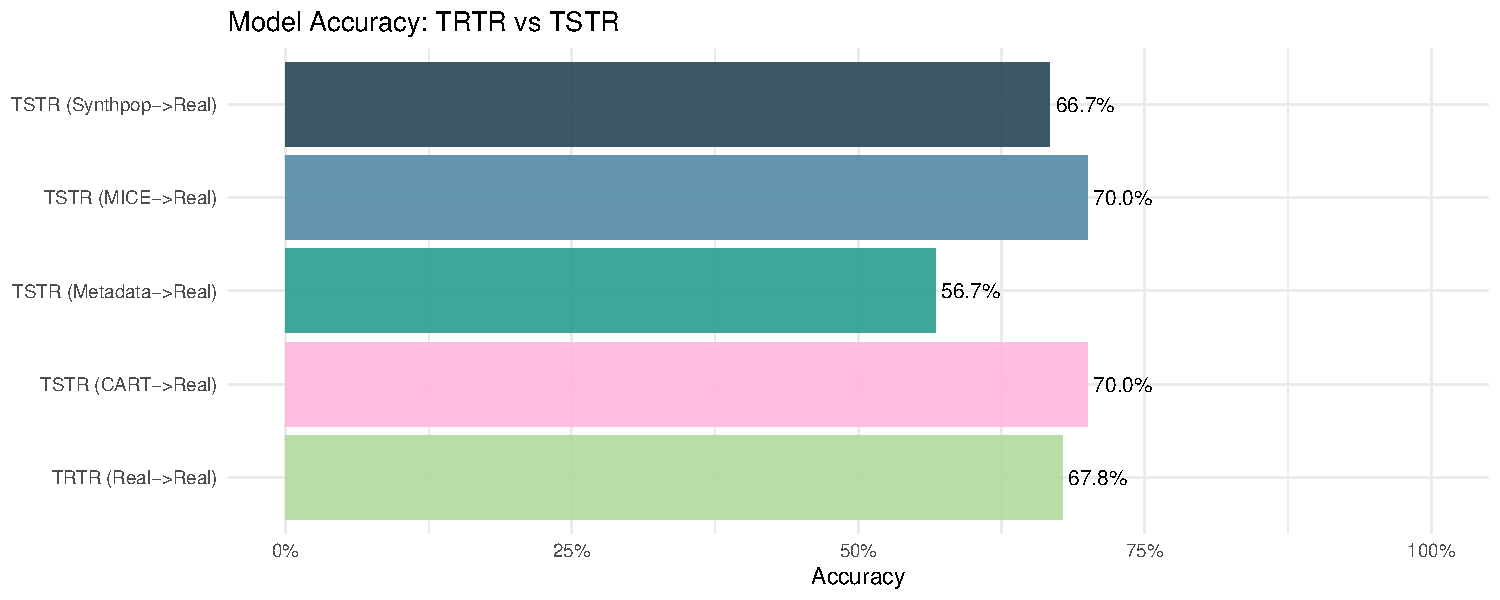
\includegraphics[width=1\linewidth,height=\textheight,keepaspectratio]{heart_failure_synthetic_data_project_files/figure-pdf/Prediction Score-1.pdf}
\end{center}

\subsubsection{Quality Score (QScore)}\label{quality-score-qscore}

The QScore provides a comprehensive evaluation of synthetic data by
aggregating multiple metrics, such as distribution similarity, feature
importance, and correlation preservation, into a single score. This
offers a clear, overall assessment of how well the synthetic data
replicates the real dataset.

Ideal Ranges for QScore:

\begin{itemize}
\tightlist
\item
  \textbf{Excellent Quality (0.8 - 1.0)}: Indicates the synthetic data
  closely mirrors the real and can be confidently used for most
  analyses.
\item
  \textbf{Good Quality (0.6 - 0.8)}: Reflects good alignment, with some
  minor deviations. Suitable for most use cases, but some caution is
  advised.
\item
  \textbf{Moderate Quality (0.4 - 0.6)}: The synthetic data may be
  useful for exploratory analysis but shows significant deviations in
  key metrics.
\item
  \textbf{Poor Quality (\textless{} 0.4)}: The synthetic data poorly
  aligns with the real and is likely unsuitable for most analytic or
  modeling tasks.
\end{itemize}

\begin{Shaded}
\begin{Highlighting}[]
\CommentTok{\# {-}{-}{-}{-} QScore helper {-}{-}{-}{-}}
\NormalTok{calculate\_qscore }\OtherTok{\textless{}{-}} \ControlFlowTok{function}\NormalTok{(real\_data, synthetic\_data, }\AttributeTok{num\_queries =} \DecValTok{10}\NormalTok{) \{}
\NormalTok{  numeric\_real\_vars  }\OtherTok{\textless{}{-}} \FunctionTok{names}\NormalTok{(real\_data)[}\FunctionTok{sapply}\NormalTok{(real\_data, is.numeric)]}
\NormalTok{  numeric\_synth\_vars }\OtherTok{\textless{}{-}} \FunctionTok{names}\NormalTok{(synthetic\_data)[}\FunctionTok{sapply}\NormalTok{(synthetic\_data, is.numeric)]}
\NormalTok{  common\_vars }\OtherTok{\textless{}{-}} \FunctionTok{intersect}\NormalTok{(numeric\_real\_vars, numeric\_synth\_vars)}
  \ControlFlowTok{if}\NormalTok{ (}\FunctionTok{length}\NormalTok{(common\_vars) }\SpecialCharTok{==} \DecValTok{0}\NormalTok{) }\FunctionTok{return}\NormalTok{(}\ConstantTok{NA\_real\_}\NormalTok{)}

\NormalTok{  qscores }\OtherTok{\textless{}{-}} \FunctionTok{replicate}\NormalTok{(num\_queries, \{}
\NormalTok{    var\_name }\OtherTok{\textless{}{-}} \FunctionTok{sample}\NormalTok{(common\_vars, }\DecValTok{1}\NormalTok{)}
\NormalTok{    fun\_name }\OtherTok{\textless{}{-}} \FunctionTok{sample}\NormalTok{(}\FunctionTok{c}\NormalTok{(}\StringTok{"mean"}\NormalTok{, }\StringTok{"sum"}\NormalTok{), }\DecValTok{1}\NormalTok{)}
\NormalTok{    fun      }\OtherTok{\textless{}{-}} \FunctionTok{match.fun}\NormalTok{(fun\_name)}

\NormalTok{    real\_val  }\OtherTok{\textless{}{-}} \FunctionTok{fun}\NormalTok{(real\_data[[var\_name]],  }\AttributeTok{na.rm =} \ConstantTok{TRUE}\NormalTok{)}
\NormalTok{    synth\_val }\OtherTok{\textless{}{-}} \FunctionTok{fun}\NormalTok{(synthetic\_data[[var\_name]], }\AttributeTok{na.rm =} \ConstantTok{TRUE}\NormalTok{)}

    \ControlFlowTok{if}\NormalTok{ (}\SpecialCharTok{!}\FunctionTok{is.na}\NormalTok{(real\_val) }\SpecialCharTok{\&\&}\NormalTok{ real\_val }\SpecialCharTok{!=} \DecValTok{0} \SpecialCharTok{\&\&} \SpecialCharTok{!}\FunctionTok{is.na}\NormalTok{(synth\_val)) \{}
      \FunctionTok{abs}\NormalTok{(real\_val }\SpecialCharTok{{-}}\NormalTok{ synth\_val) }\SpecialCharTok{/} \FunctionTok{abs}\NormalTok{(real\_val)  }\CommentTok{\# proportion difference (0–1)}
\NormalTok{    \} }\ControlFlowTok{else}\NormalTok{ \{}
      \DecValTok{0}
\NormalTok{    \}}
\NormalTok{  \})}

  \FunctionTok{mean}\NormalTok{(qscores, }\AttributeTok{na.rm =} \ConstantTok{TRUE}\NormalTok{)}
\NormalTok{\}}

\CommentTok{\# {-}{-}{-}{-} Compute and present {-}{-}{-}{-}}
\NormalTok{qscore\_tbl }\OtherTok{\textless{}{-}}\NormalTok{ tibble}\SpecialCharTok{::}\FunctionTok{tibble}\NormalTok{(}
  \AttributeTok{Dataset =} \FunctionTok{c}\NormalTok{(}\StringTok{"Parametric MICE"}\NormalTok{, }\StringTok{"CART Imputation"}\NormalTok{,}
              \StringTok{"Synthpop (Low Fidelity)"}\NormalTok{, }\StringTok{"Metadata{-}Based"}\NormalTok{),}
  \AttributeTok{QScore =} \FunctionTok{c}\NormalTok{(}
    \FunctionTok{calculate\_qscore}\NormalTok{(heart\_failure, syn\_data\_1),}
    \FunctionTok{calculate\_qscore}\NormalTok{(heart\_failure, syn\_cart\_1),}
    \FunctionTok{calculate\_qscore}\NormalTok{(heart\_failure, syn\_data\_low\_fidelity\_synthpop),}
    \FunctionTok{calculate\_qscore}\NormalTok{(heart\_failure, syn\_data\_metadata)}
\NormalTok{  )}
\NormalTok{) }\SpecialCharTok{\%\textgreater{}\%}
\NormalTok{  dplyr}\SpecialCharTok{::}\FunctionTok{mutate}\NormalTok{(}
    \AttributeTok{QScore\_num =}\NormalTok{ QScore,                                   }\CommentTok{\# keep numeric 0–1}
    \AttributeTok{QScore\_pct =}\NormalTok{ scales}\SpecialCharTok{::}\FunctionTok{percent}\NormalTok{(QScore\_num, }\AttributeTok{accuracy =} \FloatTok{0.1}\NormalTok{) }\CommentTok{\# pretty \%}
\NormalTok{  )}

\CommentTok{\# {-}{-}{-} User{-}friendly table (as percentages) {-}{-}{-}}
\NormalTok{knitr}\SpecialCharTok{::}\FunctionTok{kable}\NormalTok{(}
\NormalTok{  qscore\_tbl }\SpecialCharTok{\%\textgreater{}\%}\NormalTok{ dplyr}\SpecialCharTok{::}\FunctionTok{select}\NormalTok{(Dataset, }\StringTok{\textasciigrave{}}\AttributeTok{QScore (\%)}\StringTok{\textasciigrave{}} \OtherTok{=}\NormalTok{ QScore\_pct),}
  \AttributeTok{caption =} \StringTok{"Quality Score (QScore) — average \% difference in aggregates (lower is better)"}\NormalTok{,}
  \AttributeTok{align =} \StringTok{"lr"}
\NormalTok{)}
\end{Highlighting}
\end{Shaded}

\begin{longtable}[]{@{}lr@{}}
\caption{Quality Score (QScore) --- average \% difference in aggregates
(lower is better)}\tabularnewline
\toprule\noalign{}
Dataset & QScore (\%) \\
\midrule\noalign{}
\endfirsthead
\toprule\noalign{}
Dataset & QScore (\%) \\
\midrule\noalign{}
\endhead
\bottomrule\noalign{}
\endlastfoot
Parametric MICE & 8.8\% \\
CART Imputation & 4.7\% \\
Synthpop (Low Fidelity) & 10.6\% \\
Metadata-Based & 3.0\% \\
\end{longtable}

\begin{Shaded}
\begin{Highlighting}[]
\CommentTok{\# {-}{-}{-} Horizontal bar chart (percent axis) {-}{-}{-}}
\NormalTok{pal }\OtherTok{\textless{}{-}} \FunctionTok{c}\NormalTok{(}\StringTok{"\#B0D99B"}\NormalTok{, }\StringTok{"\#528AA8"}\NormalTok{, }\StringTok{"\#FFB6DB"}\NormalTok{, }\StringTok{"\#264653"}\NormalTok{, }\StringTok{"\#2A9D8F"}\NormalTok{)}

\FunctionTok{ggplot}\NormalTok{(qscore\_tbl, }\FunctionTok{aes}\NormalTok{(}\AttributeTok{y =}\NormalTok{ Dataset, }\AttributeTok{x =}\NormalTok{ QScore\_num, }\AttributeTok{fill =}\NormalTok{ Dataset)) }\SpecialCharTok{+}
  \FunctionTok{geom\_col}\NormalTok{(}\AttributeTok{alpha =} \FloatTok{0.9}\NormalTok{, }\AttributeTok{show.legend =} \ConstantTok{FALSE}\NormalTok{) }\SpecialCharTok{+}
  \FunctionTok{geom\_text}\NormalTok{(}\FunctionTok{aes}\NormalTok{(}\AttributeTok{label =}\NormalTok{ QScore\_pct), }\AttributeTok{hjust =} \SpecialCharTok{{-}}\FloatTok{0.1}\NormalTok{, }\AttributeTok{size =} \FloatTok{3.5}\NormalTok{) }\SpecialCharTok{+}
  \FunctionTok{scale\_fill\_manual}\NormalTok{(}\AttributeTok{values =} \FunctionTok{setNames}\NormalTok{(pal[}\FunctionTok{seq\_len}\NormalTok{(}\FunctionTok{nrow}\NormalTok{(qscore\_tbl))], qscore\_tbl}\SpecialCharTok{$}\NormalTok{Dataset)) }\SpecialCharTok{+}
  \FunctionTok{scale\_x\_continuous}\NormalTok{(}\AttributeTok{labels =}\NormalTok{ scales}\SpecialCharTok{::}\FunctionTok{percent\_format}\NormalTok{(}\AttributeTok{accuracy =} \DecValTok{1}\NormalTok{), }\AttributeTok{limits =} \FunctionTok{c}\NormalTok{(}\DecValTok{0}\NormalTok{, }\DecValTok{1}\NormalTok{),}
                     \AttributeTok{expand =} \FunctionTok{expansion}\NormalTok{(}\AttributeTok{mult =} \FunctionTok{c}\NormalTok{(}\DecValTok{0}\NormalTok{, }\FloatTok{0.05}\NormalTok{))) }\SpecialCharTok{+}
  \FunctionTok{labs}\NormalTok{(}
    \AttributeTok{title =} \StringTok{"QScore Comparison (Lower is Better)"}\NormalTok{,}
    \AttributeTok{subtitle =} \StringTok{"Average percentage difference between real and synthetic aggregates across random queries"}\NormalTok{,}
    \AttributeTok{x =} \StringTok{"QScore (\%)"}\NormalTok{, }\AttributeTok{y =} \ConstantTok{NULL}
\NormalTok{  ) }\SpecialCharTok{+}
  \FunctionTok{theme\_minimal}\NormalTok{()}
\end{Highlighting}
\end{Shaded}

\begin{center}
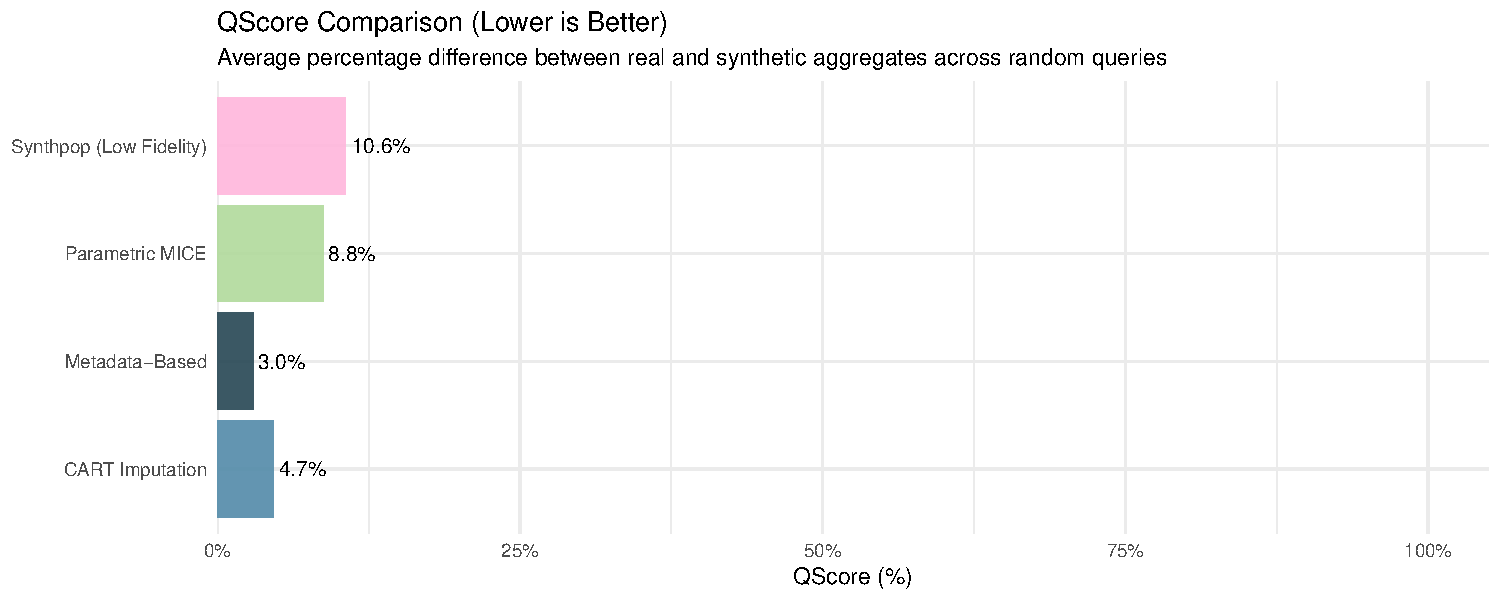
\includegraphics[width=0.99\linewidth,height=\textheight,keepaspectratio]{heart_failure_synthetic_data_project_files/figure-pdf/Quality Score-1.pdf}
\end{center}

\subsection{Privacy / Disclosure Risk}\label{privacy-disclosure-risk}

\subsubsection{Check for Replication of Real Value
Combinations}\label{check-for-replication-of-real-value-combinations}

This check identifies if any records in the synthetic data are exact
duplicates of those in the real dataset. High replication increases
privacy risks, so minimal or no duplication is ideal for preserving
privacy.

\begin{Shaded}
\begin{Highlighting}[]
\CommentTok{\# {-}{-}{-}{-} Helper: replicated rows count {-}{-}{-}{-}}
\NormalTok{check\_replicated\_rows }\OtherTok{\textless{}{-}} \ControlFlowTok{function}\NormalTok{(real\_data, synthetic\_data) \{}
\NormalTok{  combined }\OtherTok{\textless{}{-}} \FunctionTok{rbind}\NormalTok{(real\_data, synthetic\_data)}
  \FunctionTok{sum}\NormalTok{(}\FunctionTok{duplicated}\NormalTok{(combined))}
\NormalTok{\}}

\CommentTok{\# {-}{-}{-}{-} Build results table {-}{-}{-}{-}}
\NormalTok{replication\_tbl }\OtherTok{\textless{}{-}}\NormalTok{ tibble}\SpecialCharTok{::}\FunctionTok{tibble}\NormalTok{(}
  \AttributeTok{Dataset =} \FunctionTok{c}\NormalTok{(}\StringTok{"Parametric MICE"}\NormalTok{, }\StringTok{"Non{-}Parametric CART"}\NormalTok{, }
              \StringTok{"Synthpop (Low Fidelity)"}\NormalTok{, }\StringTok{"Metadata{-}Based"}\NormalTok{),}
  \AttributeTok{Replicated\_Rows =} \FunctionTok{c}\NormalTok{(}
    \FunctionTok{check\_replicated\_rows}\NormalTok{(heart\_failure, syn\_data\_1),}
    \FunctionTok{check\_replicated\_rows}\NormalTok{(heart\_failure, syn\_cart\_1),}
    \FunctionTok{check\_replicated\_rows}\NormalTok{(heart\_failure, syn\_data\_low\_fidelity\_synthpop),}
    \FunctionTok{check\_replicated\_rows}\NormalTok{(heart\_failure, syn\_data\_metadata)}
\NormalTok{  )}
\NormalTok{) }\SpecialCharTok{\%\textgreater{}\%}
  \FunctionTok{mutate}\NormalTok{(}
    \AttributeTok{Total\_Rows =} \FunctionTok{nrow}\NormalTok{(heart\_failure),}
    \AttributeTok{Replication\_Percent =} \FunctionTok{round}\NormalTok{((Replicated\_Rows }\SpecialCharTok{/}\NormalTok{ Total\_Rows) }\SpecialCharTok{*} \DecValTok{100}\NormalTok{, }\DecValTok{2}\NormalTok{),}
    \AttributeTok{Status =} \FunctionTok{ifelse}\NormalTok{(Replicated\_Rows }\SpecialCharTok{\textgreater{}} \DecValTok{0}\NormalTok{, }\StringTok{"⚠️ Replication Found"}\NormalTok{, }\StringTok{"✅ No Replication"}\NormalTok{)}
\NormalTok{  )}

\CommentTok{\# {-}{-}{-}{-} User{-}friendly table {-}{-}{-}{-}}
\NormalTok{knitr}\SpecialCharTok{::}\FunctionTok{kable}\NormalTok{(}
\NormalTok{  replication\_tbl,}
  \AttributeTok{caption =} \StringTok{"Replication Check: Exact Matching Rows Between Real and Synthetic Datasets"}\NormalTok{,}
  \AttributeTok{align =} \StringTok{"lrrrl"}
\NormalTok{)}
\end{Highlighting}
\end{Shaded}

\begin{longtable}[]{@{}
  >{\raggedright\arraybackslash}p{(\linewidth - 8\tabcolsep) * \real{0.2697}}
  >{\raggedleft\arraybackslash}p{(\linewidth - 8\tabcolsep) * \real{0.1798}}
  >{\raggedleft\arraybackslash}p{(\linewidth - 8\tabcolsep) * \real{0.1236}}
  >{\raggedleft\arraybackslash}p{(\linewidth - 8\tabcolsep) * \real{0.2247}}
  >{\raggedright\arraybackslash}p{(\linewidth - 8\tabcolsep) * \real{0.2022}}@{}}
\caption{Replication Check: Exact Matching Rows Between Real and
Synthetic Datasets}\tabularnewline
\toprule\noalign{}
\begin{minipage}[b]{\linewidth}\raggedright
Dataset
\end{minipage} & \begin{minipage}[b]{\linewidth}\raggedleft
Replicated\_Rows
\end{minipage} & \begin{minipage}[b]{\linewidth}\raggedleft
Total\_Rows
\end{minipage} & \begin{minipage}[b]{\linewidth}\raggedleft
Replication\_Percent
\end{minipage} & \begin{minipage}[b]{\linewidth}\raggedright
Status
\end{minipage} \\
\midrule\noalign{}
\endfirsthead
\toprule\noalign{}
\begin{minipage}[b]{\linewidth}\raggedright
Dataset
\end{minipage} & \begin{minipage}[b]{\linewidth}\raggedleft
Replicated\_Rows
\end{minipage} & \begin{minipage}[b]{\linewidth}\raggedleft
Total\_Rows
\end{minipage} & \begin{minipage}[b]{\linewidth}\raggedleft
Replication\_Percent
\end{minipage} & \begin{minipage}[b]{\linewidth}\raggedright
Status
\end{minipage} \\
\midrule\noalign{}
\endhead
\bottomrule\noalign{}
\endlastfoot
Parametric MICE & 0 & 299 & 0 & ✅ No Replication \\
Non-Parametric CART & 0 & 299 & 0 & ✅ No Replication \\
Synthpop (Low Fidelity) & 0 & 299 & 0 & ✅ No Replication \\
Metadata-Based & 0 & 299 & 0 & ✅ No Replication \\
\end{longtable}

\begin{Shaded}
\begin{Highlighting}[]
\CommentTok{\# {-}{-}{-}{-} Optional: bar chart if any replication \textgreater{} 0 {-}{-}{-}{-}}
\ControlFlowTok{if}\NormalTok{ (}\FunctionTok{any}\NormalTok{(replication\_tbl}\SpecialCharTok{$}\NormalTok{Replicated\_Rows }\SpecialCharTok{\textgreater{}} \DecValTok{0}\NormalTok{)) \{}
\NormalTok{  pal }\OtherTok{\textless{}{-}} \FunctionTok{c}\NormalTok{(}\StringTok{"\#B0D99B"}\NormalTok{, }\StringTok{"\#528AA8"}\NormalTok{, }\StringTok{"\#FFB6DB"}\NormalTok{, }\StringTok{"\#264653"}\NormalTok{)}
  
  \FunctionTok{ggplot}\NormalTok{(replication\_tbl, }\FunctionTok{aes}\NormalTok{(}\AttributeTok{y =}\NormalTok{ Dataset, }\AttributeTok{x =}\NormalTok{ Replicated\_Rows, }\AttributeTok{fill =}\NormalTok{ Dataset)) }\SpecialCharTok{+}
    \FunctionTok{geom\_col}\NormalTok{(}\AttributeTok{alpha =} \FloatTok{0.9}\NormalTok{, }\AttributeTok{show.legend =} \ConstantTok{FALSE}\NormalTok{) }\SpecialCharTok{+}
    \FunctionTok{geom\_text}\NormalTok{(}\FunctionTok{aes}\NormalTok{(}\AttributeTok{label =}\NormalTok{ Replicated\_Rows), }\AttributeTok{hjust =} \SpecialCharTok{{-}}\FloatTok{0.1}\NormalTok{, }\AttributeTok{size =} \FloatTok{3.5}\NormalTok{) }\SpecialCharTok{+}
    \FunctionTok{scale\_fill\_manual}\NormalTok{(}\AttributeTok{values =}\NormalTok{ pal[}\FunctionTok{seq\_len}\NormalTok{(}\FunctionTok{nrow}\NormalTok{(replication\_tbl))]) }\SpecialCharTok{+}
    \FunctionTok{labs}\NormalTok{(}
      \AttributeTok{title =} \StringTok{"Replication of Real Rows in Synthetic Data"}\NormalTok{,}
      \AttributeTok{subtitle =} \StringTok{"Counts of exact duplicated rows across real and synthetic datasets"}\NormalTok{,}
      \AttributeTok{x =} \StringTok{"Number of Replicated Rows"}\NormalTok{, }\AttributeTok{y =} \ConstantTok{NULL}
\NormalTok{    ) }\SpecialCharTok{+}
    \FunctionTok{theme\_minimal}\NormalTok{()}
\NormalTok{\} }\ControlFlowTok{else}\NormalTok{ \{}
  \FunctionTok{cat}\NormalTok{(}\StringTok{"✅ No replicated rows were found across any synthetic dataset. No plot is generated.}\SpecialCharTok{\textbackslash{}n}\StringTok{"}\NormalTok{)}
\NormalTok{\}}
\end{Highlighting}
\end{Shaded}

\begin{verbatim}
✅ No replicated rows were found across any synthetic dataset. No plot is generated.
\end{verbatim}

\subsubsection{Check for Unique Value
Combinations}\label{check-for-unique-value-combinations}

This analysis compares the number of unique row combinations between the
real and synthetic datasets. A high number of unique combinations in the
synthetic data suggests that it captures diverse patterns while
minimising the replication of sensitive information, enhancing privacy
protection.

\begin{Shaded}
\begin{Highlighting}[]
\CommentTok{\# {-}{-}{-}{-} Helper: count unique rows {-}{-}{-}{-}}
\NormalTok{unique\_combinations }\OtherTok{\textless{}{-}} \ControlFlowTok{function}\NormalTok{(data) \{}
  \FunctionTok{nrow}\NormalTok{(}\FunctionTok{unique}\NormalTok{(data))}
\NormalTok{\}}

\CommentTok{\# {-}{-}{-}{-} Build results table {-}{-}{-}{-}}
\NormalTok{unique\_tbl }\OtherTok{\textless{}{-}}\NormalTok{ tibble}\SpecialCharTok{::}\FunctionTok{tibble}\NormalTok{(}
  \AttributeTok{Dataset =} \FunctionTok{c}\NormalTok{(}\StringTok{"Real Data"}\NormalTok{, }\StringTok{"Parametric MICE"}\NormalTok{, }
              \StringTok{"Non{-}Parametric CART"}\NormalTok{, }\StringTok{"Synthpop (Low Fidelity)"}\NormalTok{, }
              \StringTok{"Metadata{-}Based"}\NormalTok{),}
  \AttributeTok{Unique\_Combinations =} \FunctionTok{c}\NormalTok{(}
    \FunctionTok{unique\_combinations}\NormalTok{(heart\_failure),}
    \FunctionTok{unique\_combinations}\NormalTok{(syn\_data\_1),}
    \FunctionTok{unique\_combinations}\NormalTok{(syn\_cart\_1),}
    \FunctionTok{unique\_combinations}\NormalTok{(syn\_data\_low\_fidelity\_synthpop),}
    \FunctionTok{unique\_combinations}\NormalTok{(syn\_data\_metadata)}
\NormalTok{  )}
\NormalTok{) }\SpecialCharTok{\%\textgreater{}\%}
  \FunctionTok{mutate}\NormalTok{(}
    \AttributeTok{Total\_Rows =} \FunctionTok{c}\NormalTok{(}\FunctionTok{nrow}\NormalTok{(heart\_failure), }\FunctionTok{rep}\NormalTok{(}\FunctionTok{nrow}\NormalTok{(heart\_failure), }\DecValTok{4}\NormalTok{)),}
    \AttributeTok{Percent\_Unique =} \FunctionTok{round}\NormalTok{((Unique\_Combinations }\SpecialCharTok{/}\NormalTok{ Total\_Rows) }\SpecialCharTok{*} \DecValTok{100}\NormalTok{, }\DecValTok{2}\NormalTok{)}
\NormalTok{  )}

\CommentTok{\# {-}{-}{-}{-} User{-}friendly table {-}{-}{-}{-}}
\NormalTok{knitr}\SpecialCharTok{::}\FunctionTok{kable}\NormalTok{(}
\NormalTok{  unique\_tbl,}
  \AttributeTok{caption =} \StringTok{"Unique Value Combinations in Real vs. Synthetic Datasets"}\NormalTok{,}
  \AttributeTok{align =} \StringTok{"lrr"}
\NormalTok{)}
\end{Highlighting}
\end{Shaded}

\begin{longtable}[]{@{}
  >{\raggedright\arraybackslash}p{(\linewidth - 6\tabcolsep) * \real{0.3429}}
  >{\raggedleft\arraybackslash}p{(\linewidth - 6\tabcolsep) * \real{0.2857}}
  >{\raggedleft\arraybackslash}p{(\linewidth - 6\tabcolsep) * \real{0.1571}}
  >{\raggedright\arraybackslash}p{(\linewidth - 6\tabcolsep) * \real{0.2143}}@{}}
\caption{Unique Value Combinations in Real vs.~Synthetic
Datasets}\tabularnewline
\toprule\noalign{}
\begin{minipage}[b]{\linewidth}\raggedright
Dataset
\end{minipage} & \begin{minipage}[b]{\linewidth}\raggedleft
Unique\_Combinations
\end{minipage} & \begin{minipage}[b]{\linewidth}\raggedleft
Total\_Rows
\end{minipage} & \begin{minipage}[b]{\linewidth}\raggedright
Percent\_Unique
\end{minipage} \\
\midrule\noalign{}
\endfirsthead
\toprule\noalign{}
\begin{minipage}[b]{\linewidth}\raggedright
Dataset
\end{minipage} & \begin{minipage}[b]{\linewidth}\raggedleft
Unique\_Combinations
\end{minipage} & \begin{minipage}[b]{\linewidth}\raggedleft
Total\_Rows
\end{minipage} & \begin{minipage}[b]{\linewidth}\raggedright
Percent\_Unique
\end{minipage} \\
\midrule\noalign{}
\endhead
\bottomrule\noalign{}
\endlastfoot
Real Data & 299 & 299 & 100 \\
Parametric MICE & 299 & 299 & 100 \\
Non-Parametric CART & 299 & 299 & 100 \\
Synthpop (Low Fidelity) & 299 & 299 & 100 \\
Metadata-Based & 299 & 299 & 100 \\
\end{longtable}

\begin{Shaded}
\begin{Highlighting}[]
\CommentTok{\# {-}{-}{-}{-} Plot only if any dataset has \textgreater{} 0 unique rows {-}{-}{-}{-}}
\ControlFlowTok{if}\NormalTok{ (}\FunctionTok{any}\NormalTok{(unique\_tbl}\SpecialCharTok{$}\NormalTok{Unique\_Combinations }\SpecialCharTok{\textgreater{}} \DecValTok{0}\NormalTok{, }\AttributeTok{na.rm =} \ConstantTok{TRUE}\NormalTok{)) \{}
\NormalTok{  pal }\OtherTok{\textless{}{-}} \FunctionTok{c}\NormalTok{(}\StringTok{"\#B0D99B"}\NormalTok{, }\StringTok{"\#528AA8"}\NormalTok{, }\StringTok{"\#FFB6DB"}\NormalTok{, }\StringTok{"\#264653"}\NormalTok{, }\StringTok{"\#2A9D8F"}\NormalTok{)}

  \FunctionTok{ggplot}\NormalTok{(unique\_tbl, }\FunctionTok{aes}\NormalTok{(}\AttributeTok{y =}\NormalTok{ Dataset, }\AttributeTok{x =}\NormalTok{ Percent\_Unique, }\AttributeTok{fill =}\NormalTok{ Dataset)) }\SpecialCharTok{+}
    \FunctionTok{geom\_col}\NormalTok{(}\AttributeTok{alpha =} \FloatTok{0.9}\NormalTok{, }\AttributeTok{show.legend =} \ConstantTok{FALSE}\NormalTok{) }\SpecialCharTok{+}
    \FunctionTok{geom\_text}\NormalTok{(}\FunctionTok{aes}\NormalTok{(}\AttributeTok{label =} \FunctionTok{paste0}\NormalTok{(Percent\_Unique, }\StringTok{"\%"}\NormalTok{)), }\AttributeTok{hjust =} \SpecialCharTok{{-}}\FloatTok{0.1}\NormalTok{, }\AttributeTok{size =} \FloatTok{3.5}\NormalTok{) }\SpecialCharTok{+}
    \FunctionTok{scale\_fill\_manual}\NormalTok{(}\AttributeTok{values =}\NormalTok{ pal[}\FunctionTok{seq\_len}\NormalTok{(}\FunctionTok{nrow}\NormalTok{(unique\_tbl))]) }\SpecialCharTok{+}
    \FunctionTok{scale\_x\_continuous}\NormalTok{(}\AttributeTok{limits =} \FunctionTok{c}\NormalTok{(}\DecValTok{0}\NormalTok{, }\DecValTok{100}\NormalTok{)) }\SpecialCharTok{+}
    \FunctionTok{labs}\NormalTok{(}
      \AttributeTok{title =} \StringTok{"Percentage of Unique Row Combinations"}\NormalTok{,}
      \AttributeTok{subtitle =} \StringTok{"Higher \% means fewer duplicates within the dataset"}\NormalTok{,}
      \AttributeTok{x =} \StringTok{"Percent of Rows that are Unique"}\NormalTok{, }\AttributeTok{y =} \ConstantTok{NULL}
\NormalTok{    ) }\SpecialCharTok{+}
    \FunctionTok{theme\_minimal}\NormalTok{()}
\NormalTok{\} }\ControlFlowTok{else}\NormalTok{ \{}
  \FunctionTok{cat}\NormalTok{(}\StringTok{"✅ No unique combinations detected across datasets.  No plot is generated. }\SpecialCharTok{\textbackslash{}n}\StringTok{"}\NormalTok{)}
\NormalTok{\}}
\end{Highlighting}
\end{Shaded}

\begin{center}
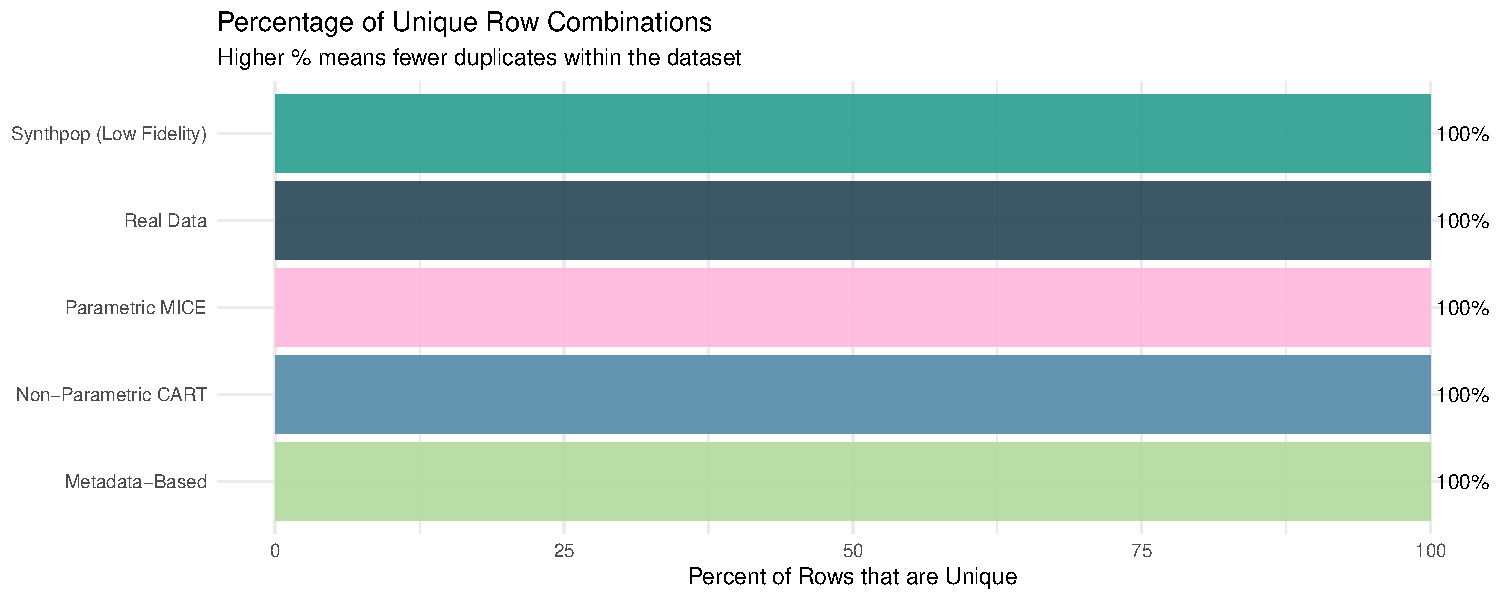
\includegraphics[width=0.99\linewidth,height=\textheight,keepaspectratio]{heart_failure_synthetic_data_project_files/figure-pdf/Check for Unique Value Combinations-1.pdf}
\end{center}

\subsubsection{Exact Match Score}\label{exact-match-score}

The Exact Match Score measures how many individual records in the
synthetic data are identical to records in the real dataset. Lower
scores are ideal for privacy preservation, as high exact matches may
pose privacy risks.

Ideal Ranges for Exact Match Score:

\begin{itemize}
\tightlist
\item
  \textbf{0 - 0.1}: Strong privacy protection with minimal or no exact
  matches, ideal for most privacy-preserving synthetic data.
\item
  \textbf{0.1 - 0.3}: Moderate exact matches, indicating some privacy
  risk but generally acceptable for many use cases.
\item
  \textbf{0.3 - 0.5}: Higher exact matches, raising privacy concerns.
  Review is needed to ensure proper data generation.
\item
  \textbf{Above 0.5}: Significant privacy risk, as the synthetic data
  too closely replicates the real.
\end{itemize}

\begin{Shaded}
\begin{Highlighting}[]
\CommentTok{\# {-}{-}{-}{-} Helper: Membership Inference Score {-}{-}{-}{-}}
\NormalTok{calculate\_membership\_inference\_score }\OtherTok{\textless{}{-}} \ControlFlowTok{function}\NormalTok{(real\_data, synthetic\_data, }\AttributeTok{k =} \DecValTok{5}\NormalTok{, }\AttributeTok{threshold =} \FloatTok{0.01}\NormalTok{) \{}
\NormalTok{  real\_num  }\OtherTok{\textless{}{-}}\NormalTok{ real\_data[}\FunctionTok{sapply}\NormalTok{(real\_data, is.numeric)]}
\NormalTok{  synth\_num }\OtherTok{\textless{}{-}}\NormalTok{ synthetic\_data[}\FunctionTok{sapply}\NormalTok{(synthetic\_data, is.numeric)]}
  \ControlFlowTok{if}\NormalTok{ (}\FunctionTok{ncol}\NormalTok{(real\_num) }\SpecialCharTok{==} \DecValTok{0} \SpecialCharTok{||} \FunctionTok{ncol}\NormalTok{(synth\_num) }\SpecialCharTok{==} \DecValTok{0}\NormalTok{) }\FunctionTok{return}\NormalTok{(}\ConstantTok{NA\_real\_}\NormalTok{)}
\NormalTok{  common }\OtherTok{\textless{}{-}} \FunctionTok{intersect}\NormalTok{(}\FunctionTok{names}\NormalTok{(real\_num), }\FunctionTok{names}\NormalTok{(synth\_num))}
  \ControlFlowTok{if}\NormalTok{ (}\FunctionTok{length}\NormalTok{(common) }\SpecialCharTok{==} \DecValTok{0}\NormalTok{) }\FunctionTok{return}\NormalTok{(}\ConstantTok{NA\_real\_}\NormalTok{)}
\NormalTok{  real\_num  }\OtherTok{\textless{}{-}}\NormalTok{ real\_num[common]}
\NormalTok{  synth\_num }\OtherTok{\textless{}{-}}\NormalTok{ synth\_num[common]}
\NormalTok{  real\_cc  }\OtherTok{\textless{}{-}}\NormalTok{ real\_num[}\FunctionTok{complete.cases}\NormalTok{(real\_num), , drop }\OtherTok{=} \ConstantTok{FALSE}\NormalTok{]}
\NormalTok{  synth\_cc }\OtherTok{\textless{}{-}}\NormalTok{ synth\_num[}\FunctionTok{complete.cases}\NormalTok{(synth\_num), , drop }\OtherTok{=} \ConstantTok{FALSE}\NormalTok{]}
  \ControlFlowTok{if}\NormalTok{ (}\FunctionTok{nrow}\NormalTok{(real\_cc) }\SpecialCharTok{\textless{}}\NormalTok{ k }\SpecialCharTok{||} \FunctionTok{nrow}\NormalTok{(synth\_cc) }\SpecialCharTok{==} \DecValTok{0}\NormalTok{) }\FunctionTok{return}\NormalTok{(}\ConstantTok{NA\_real\_}\NormalTok{)}
\NormalTok{  real\_scaled  }\OtherTok{\textless{}{-}} \FunctionTok{scale}\NormalTok{(real\_cc)}
\NormalTok{  synth\_scaled }\OtherTok{\textless{}{-}} \FunctionTok{scale}\NormalTok{(synth\_cc)}
\NormalTok{  nn }\OtherTok{\textless{}{-}}\NormalTok{ FNN}\SpecialCharTok{::}\FunctionTok{get.knnx}\NormalTok{(real\_scaled, synth\_scaled, k)}\SpecialCharTok{$}\NormalTok{nn.dist}
\NormalTok{  risky }\OtherTok{\textless{}{-}} \FunctionTok{sum}\NormalTok{(}\FunctionTok{rowMeans}\NormalTok{(nn) }\SpecialCharTok{\textless{}}\NormalTok{ threshold)}
\NormalTok{  risky }\SpecialCharTok{/} \FunctionTok{nrow}\NormalTok{(synth\_scaled)}
\NormalTok{\}}

\CommentTok{\# {-}{-}{-}{-} Results table {-}{-}{-}{-}}
\NormalTok{mis\_tbl }\OtherTok{\textless{}{-}}\NormalTok{ tibble}\SpecialCharTok{::}\FunctionTok{tibble}\NormalTok{(}
  \AttributeTok{Dataset =} \FunctionTok{c}\NormalTok{(}\StringTok{"Parametric MICE"}\NormalTok{, }\StringTok{"Non{-}Parametric CART"}\NormalTok{,}
              \StringTok{"Synthpop (Low Fidelity)"}\NormalTok{, }\StringTok{"Metadata{-}Based"}\NormalTok{),}
  \AttributeTok{Membership\_Inference\_Score =} \FunctionTok{c}\NormalTok{(}
    \FunctionTok{calculate\_membership\_inference\_score}\NormalTok{(heart\_failure, syn\_data\_1),}
    \FunctionTok{calculate\_membership\_inference\_score}\NormalTok{(heart\_failure, syn\_cart\_1),}
    \FunctionTok{calculate\_membership\_inference\_score}\NormalTok{(heart\_failure, syn\_data\_low\_fidelity\_synthpop),}
    \FunctionTok{calculate\_membership\_inference\_score}\NormalTok{(heart\_failure, syn\_data\_metadata)}
\NormalTok{  )}
\NormalTok{) }\SpecialCharTok{\%\textgreater{}\%}
  \FunctionTok{mutate}\NormalTok{(}
    \AttributeTok{Membership\_Inference\_Score =} \FunctionTok{round}\NormalTok{(Membership\_Inference\_Score, }\DecValTok{4}\NormalTok{),}
    \AttributeTok{Status =}\NormalTok{ dplyr}\SpecialCharTok{::}\FunctionTok{case\_when}\NormalTok{(}
      \FunctionTok{is.na}\NormalTok{(Membership\_Inference\_Score)              }\SpecialCharTok{\textasciitilde{}} \StringTok{"— Insufficient data"}\NormalTok{,}
\NormalTok{      Membership\_Inference\_Score }\SpecialCharTok{==} \DecValTok{0}                \SpecialCharTok{\textasciitilde{}} \StringTok{"✅ No risky memberships"}\NormalTok{,}
\NormalTok{      Membership\_Inference\_Score }\SpecialCharTok{\textless{}} \FloatTok{0.01}              \SpecialCharTok{\textasciitilde{}} \StringTok{"⚠️ Low risk"}\NormalTok{,}
      \ConstantTok{TRUE}                                           \SpecialCharTok{\textasciitilde{}} \StringTok{"❌ High risk"}
\NormalTok{    )}
\NormalTok{  )}

\CommentTok{\# {-}{-}{-}{-} User{-}friendly table {-}{-}{-}{-}}
\NormalTok{knitr}\SpecialCharTok{::}\FunctionTok{kable}\NormalTok{(}
\NormalTok{  mis\_tbl,}
  \AttributeTok{caption =} \StringTok{"Membership Inference Score: Proportion of synthetic records that are very close to real records (lower is better for privacy)"}\NormalTok{,}
  \AttributeTok{align   =} \StringTok{"lrr"}
\NormalTok{)}
\end{Highlighting}
\end{Shaded}

\begin{longtable}[]{@{}
  >{\raggedright\arraybackslash}p{(\linewidth - 4\tabcolsep) * \real{0.3200}}
  >{\raggedleft\arraybackslash}p{(\linewidth - 4\tabcolsep) * \real{0.3600}}
  >{\raggedleft\arraybackslash}p{(\linewidth - 4\tabcolsep) * \real{0.3200}}@{}}
\caption{Membership Inference Score: Proportion of synthetic records
that are very close to real records (lower is better for
privacy)}\tabularnewline
\toprule\noalign{}
\begin{minipage}[b]{\linewidth}\raggedright
Dataset
\end{minipage} & \begin{minipage}[b]{\linewidth}\raggedleft
Membership\_Inference\_Score
\end{minipage} & \begin{minipage}[b]{\linewidth}\raggedleft
Status
\end{minipage} \\
\midrule\noalign{}
\endfirsthead
\toprule\noalign{}
\begin{minipage}[b]{\linewidth}\raggedright
Dataset
\end{minipage} & \begin{minipage}[b]{\linewidth}\raggedleft
Membership\_Inference\_Score
\end{minipage} & \begin{minipage}[b]{\linewidth}\raggedleft
Status
\end{minipage} \\
\midrule\noalign{}
\endhead
\bottomrule\noalign{}
\endlastfoot
Parametric MICE & 0 & ✅ No risky memberships \\
Non-Parametric CART & 0 & ✅ No risky memberships \\
Synthpop (Low Fidelity) & 0 & ✅ No risky memberships \\
Metadata-Based & 0 & ✅ No risky memberships \\
\end{longtable}

\begin{Shaded}
\begin{Highlighting}[]
\CommentTok{\# {-}{-}{-}{-} Conditional plot {-}{-}{-}{-}}
\ControlFlowTok{if}\NormalTok{ (}\FunctionTok{any}\NormalTok{(mis\_tbl}\SpecialCharTok{$}\NormalTok{Membership\_Inference\_Score }\SpecialCharTok{\textgreater{}} \DecValTok{0}\NormalTok{, }\AttributeTok{na.rm =} \ConstantTok{TRUE}\NormalTok{)) \{}
\NormalTok{  pal }\OtherTok{\textless{}{-}} \FunctionTok{c}\NormalTok{(}\StringTok{"\#B0D99B"}\NormalTok{, }\StringTok{"\#528AA8"}\NormalTok{, }\StringTok{"\#FFB6DB"}\NormalTok{, }\StringTok{"\#264653"}\NormalTok{)}
  \FunctionTok{ggplot}\NormalTok{(mis\_tbl, }\FunctionTok{aes}\NormalTok{(}\AttributeTok{y =}\NormalTok{ Dataset, }\AttributeTok{x =}\NormalTok{ Membership\_Inference\_Score, }\AttributeTok{fill =}\NormalTok{ Dataset)) }\SpecialCharTok{+}
    \FunctionTok{geom\_col}\NormalTok{(}\AttributeTok{alpha =} \FloatTok{0.9}\NormalTok{, }\AttributeTok{show.legend =} \ConstantTok{FALSE}\NormalTok{, }\AttributeTok{na.rm =} \ConstantTok{TRUE}\NormalTok{) }\SpecialCharTok{+}
    \FunctionTok{geom\_text}\NormalTok{(}
      \FunctionTok{aes}\NormalTok{(}\AttributeTok{label =} \FunctionTok{ifelse}\NormalTok{(}\FunctionTok{is.na}\NormalTok{(Membership\_Inference\_Score), }\StringTok{"NA"}\NormalTok{,}
\NormalTok{                         scales}\SpecialCharTok{::}\FunctionTok{percent}\NormalTok{(Membership\_Inference\_Score, }\AttributeTok{accuracy =} \FloatTok{0.01}\NormalTok{))),}
      \AttributeTok{hjust =} \SpecialCharTok{{-}}\FloatTok{0.1}\NormalTok{, }\AttributeTok{size =} \FloatTok{3.5}
\NormalTok{    ) }\SpecialCharTok{+}
    \FunctionTok{scale\_fill\_manual}\NormalTok{(}\AttributeTok{values =}\NormalTok{ pal[}\FunctionTok{seq\_len}\NormalTok{(}\FunctionTok{nrow}\NormalTok{(mis\_tbl))]) }\SpecialCharTok{+}
    \FunctionTok{scale\_x\_continuous}\NormalTok{(}\AttributeTok{labels =}\NormalTok{ scales}\SpecialCharTok{::}\FunctionTok{percent\_format}\NormalTok{(}\AttributeTok{accuracy =} \DecValTok{1}\NormalTok{)) }\SpecialCharTok{+}
    \FunctionTok{labs}\NormalTok{(}
      \AttributeTok{title    =} \StringTok{"Membership Inference Score by Synthetic Method"}\NormalTok{,}
      \AttributeTok{subtitle =} \StringTok{"Lower values indicate better privacy protection"}\NormalTok{,}
      \AttributeTok{x =} \StringTok{"Score (Proportion of risky memberships)"}\NormalTok{,}
      \AttributeTok{y =} \ConstantTok{NULL}
\NormalTok{    ) }\SpecialCharTok{+}
    \FunctionTok{theme\_minimal}\NormalTok{()}
\NormalTok{\} }\ControlFlowTok{else}\NormalTok{ \{}
  \FunctionTok{cat}\NormalTok{(}\StringTok{"✅ All Membership Inference Scores are 0. No privacy risks detected, so no plot is generated}\SpecialCharTok{\textbackslash{}n}\StringTok{"}\NormalTok{)}
\NormalTok{\}}
\end{Highlighting}
\end{Shaded}

\begin{verbatim}
✅ All Membership Inference Scores are 0. No privacy risks detected, so no plot is generated
\end{verbatim}

\subsubsection{Neighbors' Privacy Score}\label{neighbors-privacy-score}

The Neighbors' Privacy Score identifies real records that are ``too
similar'' to synthetic records by using a nearest-neighbors search. This
metric helps evaluate privacy risk by detecting synthetic records that
closely resemble real data, which could compromise privacy.

Ideal Ranges for Neighbors' Privacy Score:

\begin{itemize}
\tightlist
\item
  \textbf{0 - 0.1}: Indicates strong privacy protection, with very few
  synthetic records too similar to real ones.
\item
  \textbf{0.1 - 0.3}: Moderate similarity, where privacy risk exists but
  remains within acceptable limits for many cases.
\item
  \textbf{Above 0.3}: Higher similarity, raising privacy concerns and
  requiring review to ensure the synthetic data is not too closely
  mimicking real data.
\end{itemize}

\begin{Shaded}
\begin{Highlighting}[]
\CommentTok{\# {-}{-}{-}{-} Helper: Neighbors\textquotesingle{} Privacy Score {-}{-}{-}{-}}
\NormalTok{calculate\_neighbors\_privacy\_score }\OtherTok{\textless{}{-}} \ControlFlowTok{function}\NormalTok{(real\_data, synthetic\_data, }\AttributeTok{k =} \DecValTok{5}\NormalTok{, }\AttributeTok{threshold =} \FloatTok{0.01}\NormalTok{) \{}
  \CommentTok{\# Numeric{-}only columns}
\NormalTok{  real\_num  }\OtherTok{\textless{}{-}}\NormalTok{ real\_data[}\FunctionTok{sapply}\NormalTok{(real\_data, is.numeric)]}
\NormalTok{  synth\_num }\OtherTok{\textless{}{-}}\NormalTok{ synthetic\_data[}\FunctionTok{sapply}\NormalTok{(synthetic\_data, is.numeric)]}
  
  \ControlFlowTok{if}\NormalTok{ (}\FunctionTok{ncol}\NormalTok{(real\_num) }\SpecialCharTok{==} \DecValTok{0} \SpecialCharTok{||} \FunctionTok{ncol}\NormalTok{(synth\_num) }\SpecialCharTok{==} \DecValTok{0}\NormalTok{) }\FunctionTok{return}\NormalTok{(}\ConstantTok{NA\_real\_}\NormalTok{)}
  
  \CommentTok{\# Keep only common columns}
\NormalTok{  common }\OtherTok{\textless{}{-}} \FunctionTok{intersect}\NormalTok{(}\FunctionTok{names}\NormalTok{(real\_num), }\FunctionTok{names}\NormalTok{(synth\_num))}
  \ControlFlowTok{if}\NormalTok{ (}\FunctionTok{length}\NormalTok{(common) }\SpecialCharTok{==} \DecValTok{0}\NormalTok{) }\FunctionTok{return}\NormalTok{(}\ConstantTok{NA\_real\_}\NormalTok{)}
\NormalTok{  real\_num  }\OtherTok{\textless{}{-}}\NormalTok{ real\_num[common]}
\NormalTok{  synth\_num }\OtherTok{\textless{}{-}}\NormalTok{ synth\_num[common]}
  
  \CommentTok{\# Complete cases}
\NormalTok{  real\_cc  }\OtherTok{\textless{}{-}}\NormalTok{ real\_num[}\FunctionTok{complete.cases}\NormalTok{(real\_num), , drop }\OtherTok{=} \ConstantTok{FALSE}\NormalTok{]}
\NormalTok{  synth\_cc }\OtherTok{\textless{}{-}}\NormalTok{ synth\_num[}\FunctionTok{complete.cases}\NormalTok{(synth\_num), , drop }\OtherTok{=} \ConstantTok{FALSE}\NormalTok{]}
  
  \ControlFlowTok{if}\NormalTok{ (}\FunctionTok{nrow}\NormalTok{(real\_cc) }\SpecialCharTok{\textless{}}\NormalTok{ k }\SpecialCharTok{||} \FunctionTok{nrow}\NormalTok{(synth\_cc) }\SpecialCharTok{==} \DecValTok{0}\NormalTok{) }\FunctionTok{return}\NormalTok{(}\ConstantTok{NA\_real\_}\NormalTok{)}
  
  \CommentTok{\# Standardise}
\NormalTok{  real\_scaled  }\OtherTok{\textless{}{-}} \FunctionTok{scale}\NormalTok{(real\_cc)}
\NormalTok{  synth\_scaled }\OtherTok{\textless{}{-}} \FunctionTok{scale}\NormalTok{(synth\_cc)}
  
  \CommentTok{\# k{-}NN distances from synthetic → real}
\NormalTok{  neighbors }\OtherTok{\textless{}{-}}\NormalTok{ FNN}\SpecialCharTok{::}\FunctionTok{get.knnx}\NormalTok{(real\_scaled, synth\_scaled, k)}\SpecialCharTok{$}\NormalTok{nn.dist}
  
  \CommentTok{\# Privacy risk: synthetic records "too close" to real}
\NormalTok{  close\_matches }\OtherTok{\textless{}{-}} \FunctionTok{sum}\NormalTok{(}\FunctionTok{rowMeans}\NormalTok{(neighbors) }\SpecialCharTok{\textless{}}\NormalTok{ threshold)}
\NormalTok{  score }\OtherTok{\textless{}{-}}\NormalTok{ close\_matches }\SpecialCharTok{/} \FunctionTok{nrow}\NormalTok{(synth\_scaled)}
  
  \FunctionTok{return}\NormalTok{(score)}
\NormalTok{\}}

\CommentTok{\# {-}{-}{-}{-} Build results table {-}{-}{-}{-}}
\NormalTok{neighbors\_tbl }\OtherTok{\textless{}{-}}\NormalTok{ tibble}\SpecialCharTok{::}\FunctionTok{tibble}\NormalTok{(}
  \AttributeTok{Dataset =} \FunctionTok{c}\NormalTok{(}\StringTok{"Parametric MICE"}\NormalTok{, }\StringTok{"Non{-}Parametric CART"}\NormalTok{,}
              \StringTok{"Synthpop (Low Fidelity)"}\NormalTok{, }\StringTok{"Metadata{-}Based"}\NormalTok{),}
  \AttributeTok{Neighbors\_Privacy\_Score =} \FunctionTok{c}\NormalTok{(}
    \FunctionTok{calculate\_neighbors\_privacy\_score}\NormalTok{(heart\_failure, syn\_data\_1),}
    \FunctionTok{calculate\_neighbors\_privacy\_score}\NormalTok{(heart\_failure, syn\_cart\_1),}
    \FunctionTok{calculate\_neighbors\_privacy\_score}\NormalTok{(heart\_failure, syn\_data\_low\_fidelity\_synthpop),}
    \FunctionTok{calculate\_neighbors\_privacy\_score}\NormalTok{(heart\_failure, syn\_data\_metadata)}
\NormalTok{  )}
\NormalTok{) }\SpecialCharTok{\%\textgreater{}\%}
  \FunctionTok{mutate}\NormalTok{(}
    \AttributeTok{Neighbors\_Privacy\_Score =} \FunctionTok{round}\NormalTok{(Neighbors\_Privacy\_Score, }\DecValTok{4}\NormalTok{),}
    \AttributeTok{Status =} \FunctionTok{case\_when}\NormalTok{(}
\NormalTok{      Neighbors\_Privacy\_Score }\SpecialCharTok{==} \DecValTok{0} \SpecialCharTok{\textasciitilde{}} \StringTok{"✅ No risky neighbors"}\NormalTok{,}
\NormalTok{      Neighbors\_Privacy\_Score }\SpecialCharTok{\textless{}} \FloatTok{0.01} \SpecialCharTok{\textasciitilde{}} \StringTok{"⚠️ Low risk"}\NormalTok{,}
      \ConstantTok{TRUE} \SpecialCharTok{\textasciitilde{}} \StringTok{"❌ High risk"}
\NormalTok{    )}
\NormalTok{  )}

\CommentTok{\# {-}{-}{-}{-} User{-}friendly table {-}{-}{-}{-}}
\NormalTok{knitr}\SpecialCharTok{::}\FunctionTok{kable}\NormalTok{(}
\NormalTok{  neighbors\_tbl,}
  \AttributeTok{caption =} \StringTok{"Neighbors\textquotesingle{} Privacy Score: Proportion of synthetic records too close to real records (lower is better for privacy)"}\NormalTok{,}
  \AttributeTok{align =} \StringTok{"lrr"}
\NormalTok{)}
\end{Highlighting}
\end{Shaded}

\begin{longtable}[]{@{}
  >{\raggedright\arraybackslash}p{(\linewidth - 4\tabcolsep) * \real{0.3429}}
  >{\raggedleft\arraybackslash}p{(\linewidth - 4\tabcolsep) * \real{0.3429}}
  >{\raggedleft\arraybackslash}p{(\linewidth - 4\tabcolsep) * \real{0.3143}}@{}}
\caption{Neighbors' Privacy Score: Proportion of synthetic records too
close to real records (lower is better for privacy)}\tabularnewline
\toprule\noalign{}
\begin{minipage}[b]{\linewidth}\raggedright
Dataset
\end{minipage} & \begin{minipage}[b]{\linewidth}\raggedleft
Neighbors\_Privacy\_Score
\end{minipage} & \begin{minipage}[b]{\linewidth}\raggedleft
Status
\end{minipage} \\
\midrule\noalign{}
\endfirsthead
\toprule\noalign{}
\begin{minipage}[b]{\linewidth}\raggedright
Dataset
\end{minipage} & \begin{minipage}[b]{\linewidth}\raggedleft
Neighbors\_Privacy\_Score
\end{minipage} & \begin{minipage}[b]{\linewidth}\raggedleft
Status
\end{minipage} \\
\midrule\noalign{}
\endhead
\bottomrule\noalign{}
\endlastfoot
Parametric MICE & 0 & ✅ No risky neighbors \\
Non-Parametric CART & 0 & ✅ No risky neighbors \\
Synthpop (Low Fidelity) & 0 & ✅ No risky neighbors \\
Metadata-Based & 0 & ✅ No risky neighbors \\
\end{longtable}

\begin{Shaded}
\begin{Highlighting}[]
\CommentTok{\# {-}{-}{-}{-} Plot only if any score \textgreater{} 0 {-}{-}{-}{-}}
\ControlFlowTok{if}\NormalTok{ (}\FunctionTok{any}\NormalTok{(neighbors\_tbl}\SpecialCharTok{$}\NormalTok{Neighbors\_Privacy\_Score }\SpecialCharTok{\textgreater{}} \DecValTok{0}\NormalTok{)) \{}
\NormalTok{  pal }\OtherTok{\textless{}{-}} \FunctionTok{c}\NormalTok{(}\StringTok{"\#B0D99B"}\NormalTok{, }\StringTok{"\#528AA8"}\NormalTok{, }\StringTok{"\#FFB6DB"}\NormalTok{, }\StringTok{"\#264653"}\NormalTok{)}
  
  \FunctionTok{ggplot}\NormalTok{(neighbors\_tbl, }\FunctionTok{aes}\NormalTok{(}\AttributeTok{y =}\NormalTok{ Dataset, }\AttributeTok{x =}\NormalTok{ Neighbors\_Privacy\_Score, }\AttributeTok{fill =}\NormalTok{ Dataset)) }\SpecialCharTok{+}
    \FunctionTok{geom\_col}\NormalTok{(}\AttributeTok{alpha =} \FloatTok{0.9}\NormalTok{, }\AttributeTok{show.legend =} \ConstantTok{FALSE}\NormalTok{) }\SpecialCharTok{+}
    \FunctionTok{geom\_text}\NormalTok{(}\FunctionTok{aes}\NormalTok{(}\AttributeTok{label =}\NormalTok{ Neighbors\_Privacy\_Score), }\AttributeTok{hjust =} \SpecialCharTok{{-}}\FloatTok{0.1}\NormalTok{, }\AttributeTok{size =} \FloatTok{3.5}\NormalTok{) }\SpecialCharTok{+}
    \FunctionTok{scale\_fill\_manual}\NormalTok{(}\AttributeTok{values =}\NormalTok{ pal[}\FunctionTok{seq\_len}\NormalTok{(}\FunctionTok{nrow}\NormalTok{(neighbors\_tbl))]) }\SpecialCharTok{+}
    \FunctionTok{scale\_x\_continuous}\NormalTok{(}\AttributeTok{labels =}\NormalTok{ scales}\SpecialCharTok{::}\FunctionTok{percent\_format}\NormalTok{(}\AttributeTok{accuracy =} \FloatTok{0.1}\NormalTok{)) }\SpecialCharTok{+}
    \FunctionTok{labs}\NormalTok{(}
      \AttributeTok{title =} \StringTok{"Neighbors\textquotesingle{} Privacy Score by Synthetic Method"}\NormalTok{,}
      \AttributeTok{subtitle =} \StringTok{"Lower values mean synthetic records are less likely to be close replicas of real individuals"}\NormalTok{,}
      \AttributeTok{x =} \StringTok{"Privacy Score (Proportion of risky neighbors)"}\NormalTok{, }\AttributeTok{y =} \ConstantTok{NULL}
\NormalTok{    ) }\SpecialCharTok{+}
    \FunctionTok{theme\_minimal}\NormalTok{()}
\NormalTok{\} }\ControlFlowTok{else}\NormalTok{ \{}
  \FunctionTok{cat}\NormalTok{(}\StringTok{"✅ All Neighbors\textquotesingle{} Privacy Scores are 0. No risky neighbors detected. No plot is generated.}\SpecialCharTok{\textbackslash{}n}\StringTok{"}\NormalTok{)}
\NormalTok{\}}
\end{Highlighting}
\end{Shaded}

\begin{verbatim}
✅ All Neighbors' Privacy Scores are 0. No risky neighbors detected. No plot is generated.
\end{verbatim}

\subsubsection{Membership Inference
Score}\label{membership-inference-score}

The Membership Inference Score evaluates the risk of membership
inference attacks, which attempt to determine whether a specific record
belongs to the real dataset. This metric helps assess the vulnerability
of synthetic data to privacy breaches.

Ideal Ranges for Membership Inference Score:

\begin{itemize}
\tightlist
\item
  \textbf{0 - 0.1}: Indicates low risk, where it is unlikely that
  membership inference attacks can accurately identify real records.
\item
  \textbf{0.1 - 0.3}: Moderate risk, where some vulnerability to
  membership inference exists but may still be acceptable for certain
  use cases.
\item
  \textbf{Above 0.3}: High risk, suggesting significant privacy concerns
  as the synthetic data could reveal membership information about the
  real records.
\end{itemize}

\begin{Shaded}
\begin{Highlighting}[]
\CommentTok{\# {-}{-}{-}{-} Helper: Membership Inference Score {-}{-}{-}{-}}
\CommentTok{\# Interpreted as the proportion of synthetic records that are "too close" to the real data.}
\CommentTok{\# Lower is better (safer).}
\NormalTok{calculate\_membership\_inference\_score }\OtherTok{\textless{}{-}} \ControlFlowTok{function}\NormalTok{(real\_data, synthetic\_data, }\AttributeTok{k =} \DecValTok{5}\NormalTok{, }\AttributeTok{threshold =} \FloatTok{0.01}\NormalTok{) \{}
  \CommentTok{\# Numeric{-}only columns}
\NormalTok{  real\_num  }\OtherTok{\textless{}{-}}\NormalTok{ real\_data[}\FunctionTok{sapply}\NormalTok{(real\_data, is.numeric)]}
\NormalTok{  synth\_num }\OtherTok{\textless{}{-}}\NormalTok{ synthetic\_data[}\FunctionTok{sapply}\NormalTok{(synthetic\_data, is.numeric)]}

  \CommentTok{\# Guardrails}
  \ControlFlowTok{if}\NormalTok{ (}\FunctionTok{ncol}\NormalTok{(real\_num) }\SpecialCharTok{==} \DecValTok{0} \SpecialCharTok{||} \FunctionTok{ncol}\NormalTok{(synth\_num) }\SpecialCharTok{==} \DecValTok{0}\NormalTok{) }\FunctionTok{return}\NormalTok{(}\ConstantTok{NA\_real\_}\NormalTok{)}

  \CommentTok{\# Keep only common numeric variables}
\NormalTok{  common }\OtherTok{\textless{}{-}} \FunctionTok{intersect}\NormalTok{(}\FunctionTok{names}\NormalTok{(real\_num), }\FunctionTok{names}\NormalTok{(synth\_num))}
  \ControlFlowTok{if}\NormalTok{ (}\FunctionTok{length}\NormalTok{(common) }\SpecialCharTok{==} \DecValTok{0}\NormalTok{) }\FunctionTok{return}\NormalTok{(}\ConstantTok{NA\_real\_}\NormalTok{)}
\NormalTok{  real\_num  }\OtherTok{\textless{}{-}}\NormalTok{ real\_num[common]}
\NormalTok{  synth\_num }\OtherTok{\textless{}{-}}\NormalTok{ synth\_num[common]}

  \CommentTok{\# Use complete cases}
\NormalTok{  real\_cc  }\OtherTok{\textless{}{-}}\NormalTok{ real\_num[}\FunctionTok{complete.cases}\NormalTok{(real\_num), , drop }\OtherTok{=} \ConstantTok{FALSE}\NormalTok{]}
\NormalTok{  synth\_cc }\OtherTok{\textless{}{-}}\NormalTok{ synth\_num[}\FunctionTok{complete.cases}\NormalTok{(synth\_num), , drop }\OtherTok{=} \ConstantTok{FALSE}\NormalTok{]}
  \ControlFlowTok{if}\NormalTok{ (}\FunctionTok{nrow}\NormalTok{(real\_cc) }\SpecialCharTok{\textless{}}\NormalTok{ k }\SpecialCharTok{||} \FunctionTok{nrow}\NormalTok{(synth\_cc) }\SpecialCharTok{==} \DecValTok{0}\NormalTok{) }\FunctionTok{return}\NormalTok{(}\ConstantTok{NA\_real\_}\NormalTok{)}

  \CommentTok{\# Standardize}
\NormalTok{  real\_scaled  }\OtherTok{\textless{}{-}} \FunctionTok{scale}\NormalTok{(real\_cc)}
\NormalTok{  synth\_scaled }\OtherTok{\textless{}{-}} \FunctionTok{scale}\NormalTok{(synth\_cc)}

  \CommentTok{\# k{-}NN distances from synthetic → real}
\NormalTok{  nn }\OtherTok{\textless{}{-}}\NormalTok{ FNN}\SpecialCharTok{::}\FunctionTok{get.knnx}\NormalTok{(real\_scaled, synth\_scaled, k)}\SpecialCharTok{$}\NormalTok{nn.dist}

  \CommentTok{\# Score: proportion of synthetic records whose average distance to k nearest reals is below threshold}
\NormalTok{  risky }\OtherTok{\textless{}{-}} \FunctionTok{sum}\NormalTok{(}\FunctionTok{rowMeans}\NormalTok{(nn) }\SpecialCharTok{\textless{}}\NormalTok{ threshold)}
\NormalTok{  risky }\SpecialCharTok{/} \FunctionTok{nrow}\NormalTok{(synth\_scaled)}
\NormalTok{\}}

\CommentTok{\# {-}{-}{-}{-} Results table {-}{-}{-}{-}}
\NormalTok{mis\_tbl }\OtherTok{\textless{}{-}}\NormalTok{ tibble}\SpecialCharTok{::}\FunctionTok{tibble}\NormalTok{(}
  \AttributeTok{Dataset =} \FunctionTok{c}\NormalTok{(}\StringTok{"Parametric MICE"}\NormalTok{, }\StringTok{"Non{-}Parametric CART"}\NormalTok{,}
              \StringTok{"Synthpop (Low Fidelity)"}\NormalTok{, }\StringTok{"Metadata{-}Based"}\NormalTok{),}
  \AttributeTok{Membership\_Inference\_Score =} \FunctionTok{c}\NormalTok{(}
    \FunctionTok{calculate\_membership\_inference\_score}\NormalTok{(heart\_failure, syn\_data\_1),}
    \FunctionTok{calculate\_membership\_inference\_score}\NormalTok{(heart\_failure, syn\_cart\_1),}
    \FunctionTok{calculate\_membership\_inference\_score}\NormalTok{(heart\_failure, syn\_data\_low\_fidelity\_synthpop),}
    \FunctionTok{calculate\_membership\_inference\_score}\NormalTok{(heart\_failure, syn\_data\_metadata)}
\NormalTok{  )}
\NormalTok{) }\SpecialCharTok{\%\textgreater{}\%}
  \FunctionTok{mutate}\NormalTok{(}
    \AttributeTok{Membership\_Inference\_Score =} \FunctionTok{round}\NormalTok{(Membership\_Inference\_Score, }\DecValTok{4}\NormalTok{),}
    \AttributeTok{Status =}\NormalTok{ dplyr}\SpecialCharTok{::}\FunctionTok{case\_when}\NormalTok{(}
      \FunctionTok{is.na}\NormalTok{(Membership\_Inference\_Score)              }\SpecialCharTok{\textasciitilde{}} \StringTok{"— Insufficient data"}\NormalTok{,}
\NormalTok{      Membership\_Inference\_Score }\SpecialCharTok{==} \DecValTok{0}                \SpecialCharTok{\textasciitilde{}} \StringTok{"✅ No risky memberships"}\NormalTok{,}
\NormalTok{      Membership\_Inference\_Score }\SpecialCharTok{\textless{}} \FloatTok{0.01}              \SpecialCharTok{\textasciitilde{}} \StringTok{"⚠️ Low risk"}\NormalTok{,}
      \ConstantTok{TRUE}                                           \SpecialCharTok{\textasciitilde{}} \StringTok{"❌ High risk"}
\NormalTok{    )}
\NormalTok{  )}

\CommentTok{\# {-}{-}{-}{-} User{-}friendly table {-}{-}{-}{-}}
\NormalTok{knitr}\SpecialCharTok{::}\FunctionTok{kable}\NormalTok{(}
\NormalTok{  mis\_tbl,}
  \AttributeTok{caption =} \StringTok{"Membership Inference Score: Proportion of synthetic records that are very close to real records (lower is better for privacy)"}\NormalTok{,}
  \AttributeTok{align   =} \StringTok{"lrr"}
\NormalTok{)}
\end{Highlighting}
\end{Shaded}

\begin{longtable}[]{@{}
  >{\raggedright\arraybackslash}p{(\linewidth - 4\tabcolsep) * \real{0.3200}}
  >{\raggedleft\arraybackslash}p{(\linewidth - 4\tabcolsep) * \real{0.3600}}
  >{\raggedleft\arraybackslash}p{(\linewidth - 4\tabcolsep) * \real{0.3200}}@{}}
\caption{Membership Inference Score: Proportion of synthetic records
that are very close to real records (lower is better for
privacy)}\tabularnewline
\toprule\noalign{}
\begin{minipage}[b]{\linewidth}\raggedright
Dataset
\end{minipage} & \begin{minipage}[b]{\linewidth}\raggedleft
Membership\_Inference\_Score
\end{minipage} & \begin{minipage}[b]{\linewidth}\raggedleft
Status
\end{minipage} \\
\midrule\noalign{}
\endfirsthead
\toprule\noalign{}
\begin{minipage}[b]{\linewidth}\raggedright
Dataset
\end{minipage} & \begin{minipage}[b]{\linewidth}\raggedleft
Membership\_Inference\_Score
\end{minipage} & \begin{minipage}[b]{\linewidth}\raggedleft
Status
\end{minipage} \\
\midrule\noalign{}
\endhead
\bottomrule\noalign{}
\endlastfoot
Parametric MICE & 0 & ✅ No risky memberships \\
Non-Parametric CART & 0 & ✅ No risky memberships \\
Synthpop (Low Fidelity) & 0 & ✅ No risky memberships \\
Metadata-Based & 0 & ✅ No risky memberships \\
\end{longtable}

\begin{Shaded}
\begin{Highlighting}[]
\CommentTok{\# {-}{-}{-}{-} Plot only if any risky memberships (\textgreater{} 0) {-}{-}{-}{-}}
\ControlFlowTok{if}\NormalTok{ (}\FunctionTok{any}\NormalTok{(mis\_tbl}\SpecialCharTok{$}\NormalTok{Membership\_Inference\_Score }\SpecialCharTok{\textgreater{}} \DecValTok{0}\NormalTok{, }\AttributeTok{na.rm =} \ConstantTok{TRUE}\NormalTok{)) \{}
\NormalTok{  pal }\OtherTok{\textless{}{-}} \FunctionTok{c}\NormalTok{(}\StringTok{"\#B0D99B"}\NormalTok{, }\StringTok{"\#528AA8"}\NormalTok{, }\StringTok{"\#FFB6DB"}\NormalTok{, }\StringTok{"\#264653"}\NormalTok{)}
  
  \FunctionTok{ggplot}\NormalTok{(mis\_tbl, }\FunctionTok{aes}\NormalTok{(}\AttributeTok{y =}\NormalTok{ Dataset, }\AttributeTok{x =}\NormalTok{ Membership\_Inference\_Score, }\AttributeTok{fill =}\NormalTok{ Dataset)) }\SpecialCharTok{+}
    \FunctionTok{geom\_col}\NormalTok{(}\AttributeTok{alpha =} \FloatTok{0.9}\NormalTok{, }\AttributeTok{show.legend =} \ConstantTok{FALSE}\NormalTok{, }\AttributeTok{na.rm =} \ConstantTok{TRUE}\NormalTok{) }\SpecialCharTok{+}
    \FunctionTok{geom\_text}\NormalTok{(}
      \FunctionTok{aes}\NormalTok{(}\AttributeTok{label =} \FunctionTok{ifelse}\NormalTok{(}\FunctionTok{is.na}\NormalTok{(Membership\_Inference\_Score), }\StringTok{"NA"}\NormalTok{,}
\NormalTok{                         scales}\SpecialCharTok{::}\FunctionTok{percent}\NormalTok{(Membership\_Inference\_Score, }\AttributeTok{accuracy =} \FloatTok{0.01}\NormalTok{))),}
      \AttributeTok{hjust =} \SpecialCharTok{{-}}\FloatTok{0.1}\NormalTok{, }\AttributeTok{size =} \FloatTok{3.5}
\NormalTok{    ) }\SpecialCharTok{+}
    \FunctionTok{scale\_fill\_manual}\NormalTok{(}\AttributeTok{values =}\NormalTok{ pal[}\FunctionTok{seq\_len}\NormalTok{(}\FunctionTok{nrow}\NormalTok{(mis\_tbl))]) }\SpecialCharTok{+}
    \FunctionTok{scale\_x\_continuous}\NormalTok{(}\AttributeTok{labels =}\NormalTok{ scales}\SpecialCharTok{::}\FunctionTok{percent\_format}\NormalTok{(}\AttributeTok{accuracy =} \DecValTok{1}\NormalTok{)) }\SpecialCharTok{+}
    \FunctionTok{labs}\NormalTok{(}
      \AttributeTok{title    =} \StringTok{"Membership Inference Score by Synthetic Method"}\NormalTok{,}
      \AttributeTok{subtitle =} \StringTok{"Lower values indicate better privacy protection"}\NormalTok{,}
      \AttributeTok{x =} \StringTok{"Score (Proportion of risky memberships)"}\NormalTok{,}
      \AttributeTok{y =} \ConstantTok{NULL}
\NormalTok{    ) }\SpecialCharTok{+}
    \FunctionTok{theme\_minimal}\NormalTok{()}
\NormalTok{\} }\ControlFlowTok{else}\NormalTok{ \{}
  \FunctionTok{cat}\NormalTok{(}\StringTok{"✅ All Membership Inference Scores are 0. No risky memberships detected. No plot is generated. }\SpecialCharTok{\textbackslash{}n}\StringTok{"}\NormalTok{)}
\NormalTok{\}}
\end{Highlighting}
\end{Shaded}

\begin{verbatim}
✅ All Membership Inference Scores are 0. No risky memberships detected. No plot is generated. 
\end{verbatim}

\subsection{Conclusions}\label{conclusions}

This report evaluated the fidelity, utility, privacy, and overall
quality of synthetic data generated using parametric MICE,
non-parametric CART, Synthpop, and metadata-based methods. Key findings
include:

\begin{itemize}
\tightlist
\item
  \textbf{Data Structure Preservation}: All methods preserved the
  structure of the real dataset, though minor variations in variable
  distributions were observed.
\item
  \textbf{Categorical Variables}: Most synthetic datasets retained
  categorical levels, but frequency distribution discrepancies were
  particularly notable in Synthpop data.
\item
  \textbf{Numeric Variables}: The range and distribution of numeric
  variables were largely maintained across methods, with slight
  variations in density plots.
\item
  \textbf{Correlation \& Mutual Information}: While most methods
  captured variable relationships, weaker correlations and lower mutual
  information scores suggested some loss of feature dependencies in
  certain synthetic datasets.
\item
  \textbf{Utility (Prediction Score)}: Synthetic data performed
  similarly to real data in predictive modeling, though slight
  reductions in accuracy and increased pMSE indicated less precise
  representation of the real dataset's predictive capabilities.
\item
  \textbf{Privacy (Exact Match \& Neighbors' Privacy Scores)}: All
  synthetic datasets demonstrated strong privacy protection, with zero
  values for both Exact Match and Neighbors' Privacy Scores. This
  indicates that no synthetic records were identical to or highly
  similar to any real records, affirming robust privacy across all
  methods.
\end{itemize}

In conclusion, synthetic data generated through these methods provides a
balance between utility and privacy, though method selection should
align with specific analytic or privacy needs.

\begin{Shaded}
\begin{Highlighting}[]
\CommentTok{\# Stop the parallel cluster}
\FunctionTok{stopCluster}\NormalTok{(cl)}
\FunctionTok{registerDoSEQ}\NormalTok{()}
\end{Highlighting}
\end{Shaded}





\end{document}
